\documentclass[a4paper,12pt]{article}  % Clase de documento

% Paquetes esenciales
\usepackage[utf8]{inputenc}         % Codificación UTF-8
\usepackage[T1]{fontenc}            % Soporte para caracteres en PDF
\usepackage[main=spanish]{babel}    % Traducir a español titulos y otros elementos
\usepackage{amsmath, amssymb}       % Matemáticas avanzadas
\usepackage{graphicx}               % Para incluir imágenes
\usepackage{wrapfig}
\usepackage{subcaption}
\usepackage[most]{tcolorbox}
\usepackage[table]{xcolor}          % Colores
\usepackage{hyperref}               % Enlaces internos y externos
\usepackage{siunitx}                % Unidades SI
\usepackage{physics}                % Notación de física
\usepackage{array, colortbl}        % Tablas
\usepackage{soul}                   % Resaltado de texto
\usepackage{enumitem}               % Listas personalizadas (itemize, enumerate)

% Configuración de siunitx para evitar conflictos con physics
\ExplSyntaxOn
\msg_redirect_name:nnn{siunitx}{physics-pkg}{none}
\ExplSyntaxOff

% Configuración de formato
\usepackage{xcolor}
\usepackage{titlesec}

% Definir colores personalizados
\definecolor{dark_blue}{RGB}{0, 102, 204}
\definecolor{dark_red}{RGB}{204, 0, 0}
\definecolor{soft_green}{RGB}{0, 153, 0}
\definecolor{intense_blue}{RGB}{30, 144, 255}
\definecolor{highlight}{RGB}{255, 230, 153}
% https://latexcolor.com/
\definecolor{brandeisblue}{rgb}{0.0, 0.44, 1.0}
\definecolor{asparagus}{rgb}{0.53, 0.66, 0.42}


\sethlcolor{highlight}
% Cambiar el color de los títulos
\titleformat{\section}
  {\color{dark_blue}\normalfont\Large\bfseries} % Estilo del título de sección
  {\thesection}{1em}{} % Numeración y espacio

\titleformat{\subsection}
  {\color{dark_red}\normalfont\large\bfseries} % Estilo del título de subsección
  {\thesubsection}{1em}{}

\titleformat{\subsubsection}
  {\color{soft_green}\normalfont\normalsize\bfseries} % Estilo del título de subsubsección
  {\thesubsubsection}{1em}{}

\renewcommand{\paragraph}[1]{%
  \noindent\textcolor{orange!70!black}{\textbf{#1}}%
  \hspace{1.2em}%
}

% Configuración de las listas
\setlist{noitemsep} % Eliminar espacio entre elementos de las listas
\setlist[itemize]{label=\textbullet} % Cambiar el símbolo de las listas itemize


% Definir comandos personalizados
\newcommand{\vect}[1]{\mathbf{#1}} % Vectores en negrita
\newcommand{\diff}[2]{\frac{d#1}{d#2}} % Derivada
\newcommand{\pdiff}[2]{\frac{\partial #1}{\partial #2}} % Derivada parcial


\hypersetup{
    colorlinks=true,
    linkcolor=black,
    urlcolor=intense_blue,
    citecolor=black
}   % Archivo de estilos personalizados (opcional)

% Directorio de imágenes por defecto.
\graphicspath{ {./images/} }

\begin{document}

\title{Física II}
\author{Elio Valentino Anci}
\date{\today}
\maketitle
\begin{figure}[ht]
    \centering
    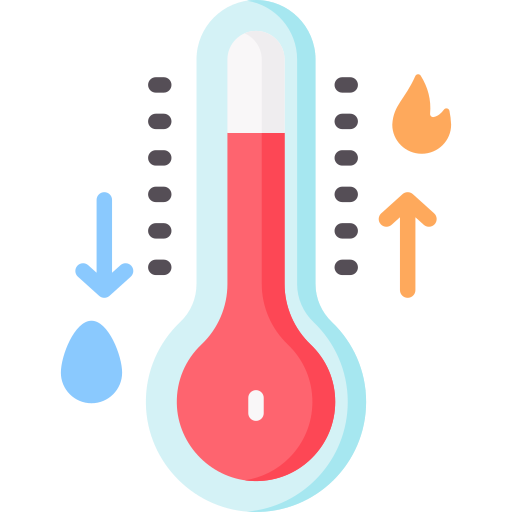
\includegraphics[width=0.3\textwidth]{images/cover.png}
\end{figure}
\newpage

\tableofcontents  % Genera tabla de contenidos automáticamente

\newpage

% Inclusión de capítulos
\section{Electrostática}

La teoría electromagnética clásica estudia los fenómenos eléctricos y magnéticos, \hl{describiendo} sus características y las \hl{leyes} que los gobiernan.  

Cuando hablamos de \textbf{teoría clásica}, nos referimos a que se basa en la mecánica clásica de Isaac Newton. En esta mecánica se utilizan conceptos como partículas, trayectorias y las leyes del movimiento de Newton. De manera similar, en la teoría electromagnética se aplican estos conceptos a las cargas eléctricas y a los campos eléctricos y magnéticos. Es decir, en lugar de hablar solo de partículas y fuerzas mecánicas, hablaremos de \textbf{partículas cargadas, fuerzas eléctricas y campos electromagnéticos}.  

El electromagnetismo es una \hl{teoría de campos}. Por ejemplo, una \textbf{carga eléctrica} genera un \textbf{campo eléctrico} a su alrededor, mientras que un \textbf{imán} produce un \textbf{campo magnético} en el espacio que lo rodea. Estos campos son \hl{perturbaciones en el espacio} que afectan a otras cargas o imanes cercanos y pueden describirse matemáticamente.  

A lo largo de la historia, se ha comprobado que existen dos tipos de carga eléctrica: \textbf{positiva} y \textbf{negativa}. Las cargas del mismo tipo se repelen, mientras que las de signos opuestos se atraen.  

\subsection{Carga y Materia}

\subsection{Carga y Materia}

Todo lo que nos rodea, como una pelota, el aire, una planta o nuestro propio cuerpo, está formado por \textbf{átomos}. Los átomos, a su vez, están compuestos por tres tipos de partículas: \textbf{protones, neutrones y electrones}. Los protones y neutrones se encuentran en el núcleo del átomo, mientras que los electrones se mueven alrededor en la corteza. Los protones tienen \hl{carga positiva}, los electrones \hl{carga negativa}, y los neutrones no tienen carga. 

\begin{figure}[ht]
    \centering
    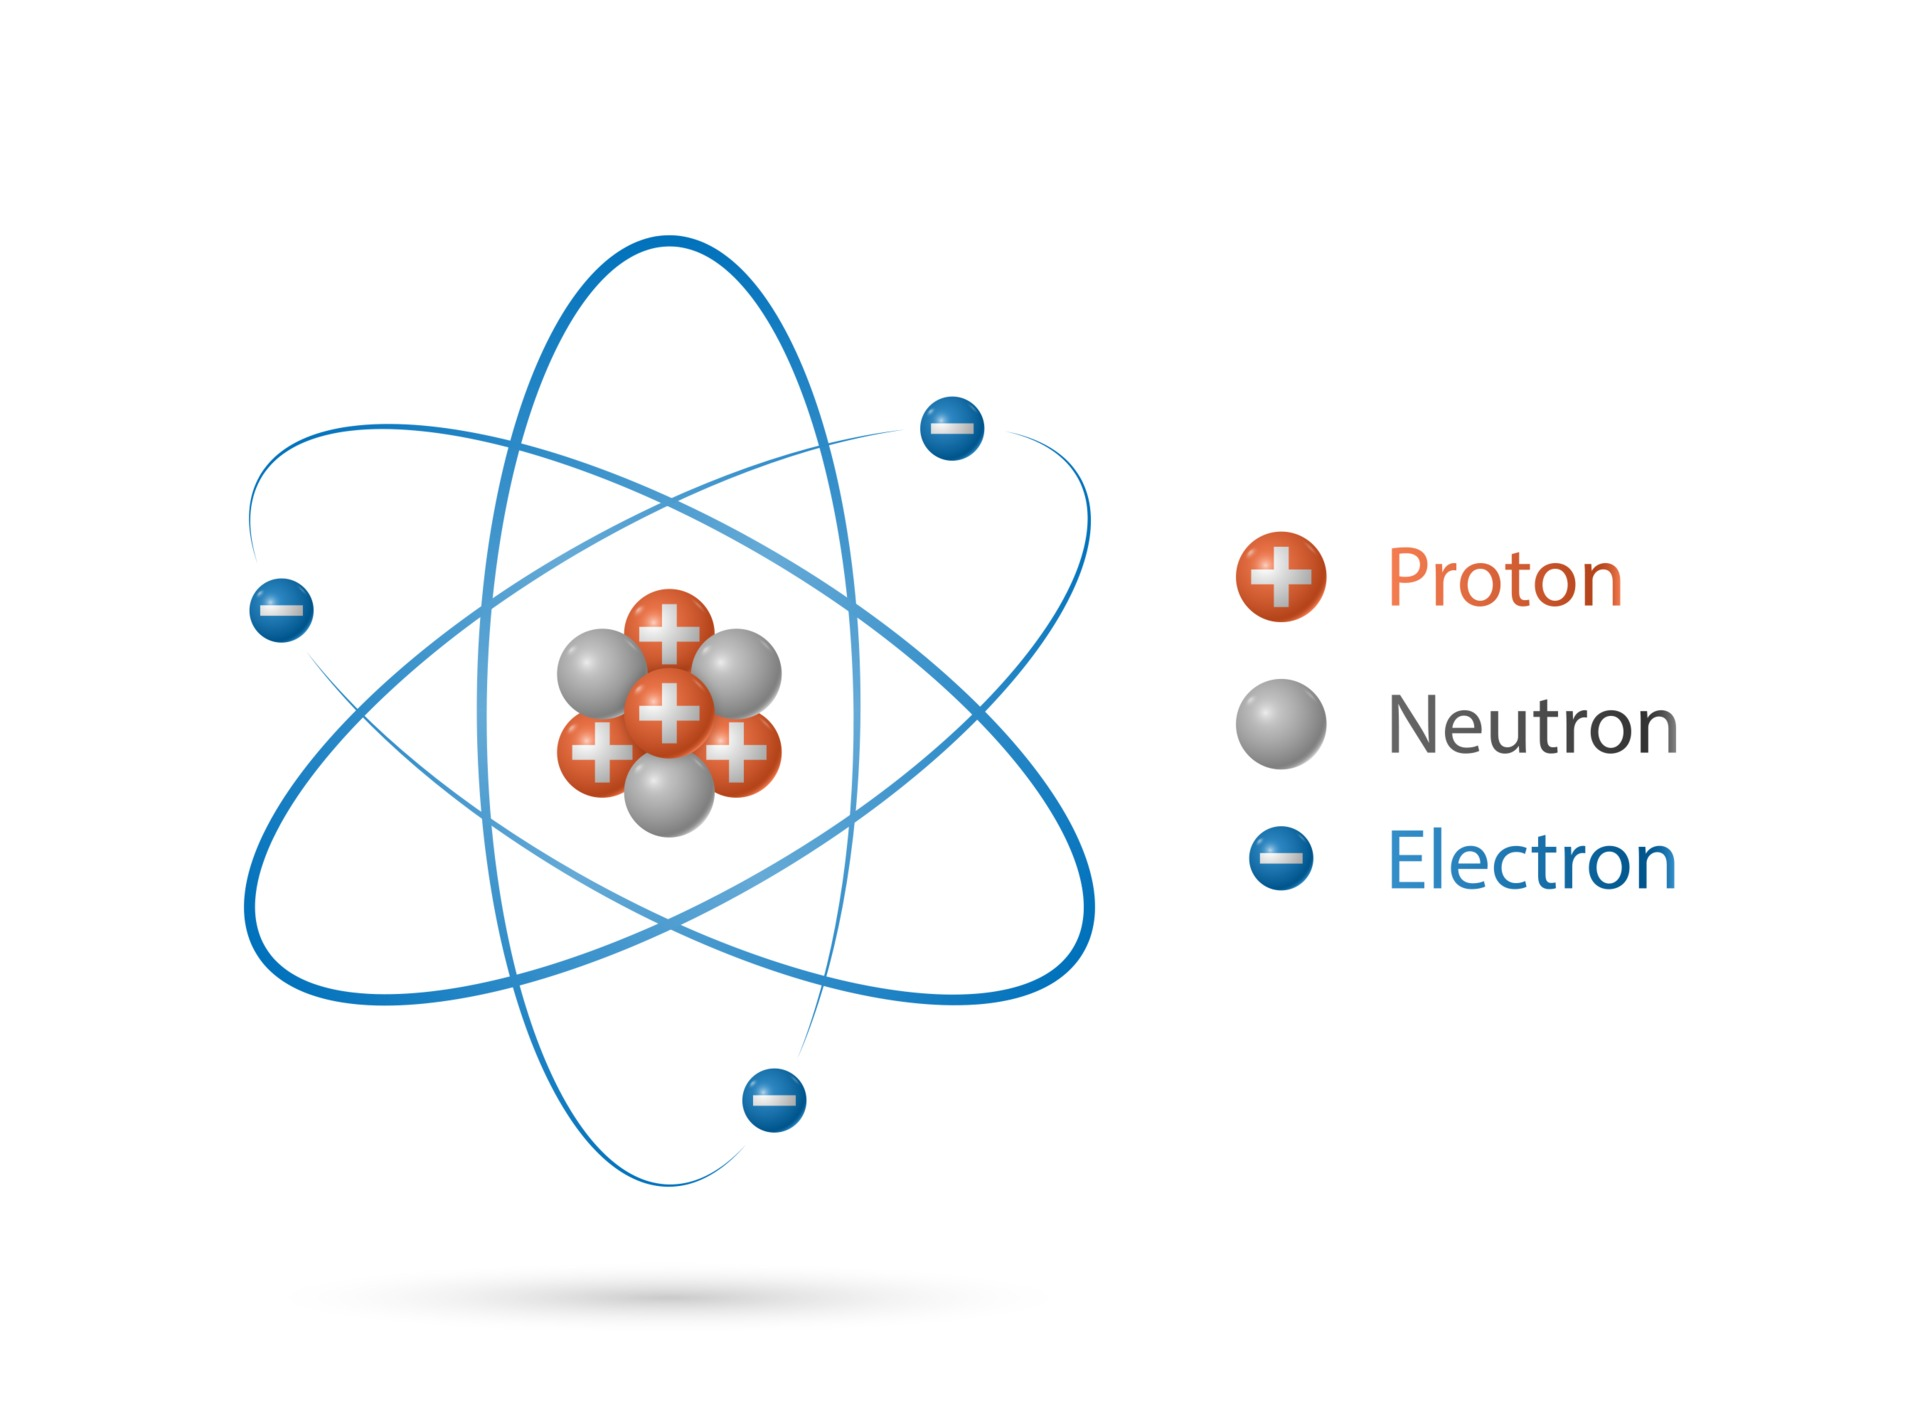
\includegraphics[width=0.4\textwidth]{atom_struct.jpg}
    \caption{Estructura básica de un átomo.}
    \label{fig:atom_struct}
\end{figure}

Esta estructura corresponde a un \textbf{modelo atómico}, que es una representación que nos ayuda a entender cómo está compuesto un átomo y cómo se comporta. A lo largo del tiempo han existido distintos modelos atómicos, pero uno de los más conocidos es el \textbf{modelo de Bohr}. Según este modelo, los electrones giran alrededor del núcleo en \textbf{órbitas circulares}, cada una con un nivel de energía específico. Cuando un electrón cambia de órbita, absorbe o emite energía en forma de luz.

La carga elemental \colorbox{highlight}{\( e \)} es la \textbf{cantidad más pequeña de carga eléctrica libre que se conoce en la naturaleza}. Es la carga que poseen los protones y electrones, pero con signo opuesto:
\begin{itemize}
    \item \textbf{Electrón}: \( -e = -1.602 \times 10^{-19} \) C (coulombs)
    \item \textbf{Protón}: \( +e = 1.602 \times 10^{-19} \) C
\end{itemize}

La carga elemental es fundamental porque todas las cargas eléctricas observadas en la naturaleza son \textbf{múltiplos enteros de \( e \)}. Es decir, cualquier carga presente en un objeto es el resultado de un exceso o déficit de electrones. Este principio se conoce como la \textbf{ley de conservación de la carga eléctrica}, y establece que la carga eléctrica \textbf{no se crea ni se destruye}, solo se transfiere de un cuerpo a otro.  

Los objetos tienen carga debido a la presencia de \textbf{electrones y protones}. Un objeto es eléctricamente neutro cuando tiene igual número de ambos. Si un objeto adquiere carga negativa, significa que ha \textbf{ganado electrones}, y si adquiere carga positiva, significa que ha \textbf{perdido electrones}. Cuando un objeto se carga, no se están creando nuevas cargas, sino que \textbf{se están moviendo electrones} de un cuerpo a otro. Por ejemplo: en la \textbf{electrización por frotamiento}, un material transfiere electrones a otro, dejando uno cargado positivamente y el otro negativamente. En la \textbf{inducción}, un objeto cargado puede redistribuir las cargas en otro sin tocarlo, pero sin cambiar la cantidad total de carga en el sistema.

En otras palabras, la carga eléctrica siempre se conserva porque \textbf{los electrones y protones no se destruyen en procesos normales}, solo cambian de ubicación dentro de un sistema.

\colorbox{highlight}{Denominaremos con la letra \( Q \) o \( q \) a la carga eléctrica de un objeto.} La carga se mide en \textbf{coulombs (C)}. Un coulomb es una cantidad de carga muy grande, por lo que en la práctica se utilizan submúltiplos como el \textbf{millicoulomb (mC)} o el \textbf{microcoulomb (\( \mu \text{C} \))}.

\subsubsection{Ley de Coulomb}

La electrostática estudia las cargas eléctricas en \hl{\textbf{reposo}}. La ley de Coulomb establece que \textbf{la fuerza entre dos cargas puntuales} es:

\begin{equation}
    F = k_e \frac{\abs{q_1} \cdot \abs{q_2}}{r^2}
    \label{eq:ley_coulomb}
\end{equation}

donde:

\begin{itemize}
    \item \( k_e \) es la constante de Coulomb: \( 8.9876 \times 10^9 \, \frac{\si{\newton\meter\squared}}{\si{\coulomb\squared}} \).
    \begin{itemize}
        \item \( k_e \) se obtiene de  \( \frac{1}{4\pi\epsilon_0} \) y,
        \item \( \epsilon_0 \) es la permitividad del vacío: \( 8.85 \times 10^{-12} \,\frac{\si{\coulomb\squared}}{\si{\newton\meter\squared}} \)
    \end{itemize}
    \item \( q_1 \) y \( q_2 \) son las cargas.
    \item \( r \) es la distancia entre las cargas.
\end{itemize}

Es muy importante notar que la \textbf{Ley de Coulomb} \eqref{eq:ley_coulomb} se aplica estrictamente a \hl{cargas puntuales}, es decir, cargas que se consideran concentradas en un solo punto sin dimensiones espaciales. En la ecuación anterior \eqref{eq:ley_coulomb}, se obtiene la magnitud de la fuerza eléctrica. La expresión vectorial de la fuerza eléctrica es:

\begin{equation}
    \vec{F}_e = k_e \frac{|q_1 q_2|}{r^2} \hat{r}
    \label{eq:ley_coulomb_vectorial}
\end{equation}

donde:
\begin{itemize}
    \item \( \vec{F}_e \) es el vector fuerza eléctrica entre dos cargas puntuales \( q_1 \) y \( q_2 \)
    \item \( \hat{r} \) es el vector unitario en la dirección que une ambas cargas.
\end{itemize}

Esto es importante tenerlo en cuenta ya que si se quiere saber la fuerza total sobre una carga \( q \) debido a varias cargas, se debe sumar vectorialmente las fuerzas individuales. La fuerza total sobre una carga \( q \) debido a un conjunto de cargas \( Q_i \) es:

\begin{equation}
    \vec{F} = \sum_i k \frac{|q \cdot Q_i|}{r_i^2} \hat{\mathbf{r_i}}
    \label{eq:ley_coulomb_vectorial_suma}
\end{equation}

\subsubsection{Cargas eléctricas}

La \textbf{carga eléctrica} es una propiedad fundamental de la materia que determina la interacción electromagnética entre partículas. Se trata de una magnitud escalar que puede ser de dos tipos: \textbf{positiva} o \textbf{negativa}. Las partículas con carga del mismo signo se repelen, mientras que las de signo opuesto se atraen.

La unidad de carga eléctrica en el \textbf{Sistema Internacional (SI)} es el \textbf{coulomb (\( \si{coulomb} \))}. La carga elemental está representada por la carga del electrón (\( -e = -1.602 \times 10^{-19} \si{coulomb} \)) y la del protón (\( e = +1.602 \times 10^{-19} \si{coulomb} \)).

\begin{center}
    \setlength{\arrayrulewidth}{1pt}  % Grosor de líneas
    \renewcommand{\arraystretch}{1.3} % Espaciado vertical
    \arrayrulecolor{gray} % Color de líneas

    \begin{tabular}{ c c c }
        \hline
        \rowcolor{asparagus!30}
        \textbf{Partícula}  & \textbf{Carga (\si{C})}           & \textbf{Masa (\si{kg})}   \\ \hline
        Electrón (e)        & \(-e = -1.602 \times 10^{-19}\)   & \(9.109 \times 10^{-31}\) \\
        Protón (p)          & \(+e = +1.602 \times 10^{-19}\)   & \(1.672 \times 10^{-27}\) \\
        Neutrón (n)         & \(0\)                             & \(1.675 \times 10^{-27}\) \\ \hline
    \end{tabular}
\end{center}

\subsubsection{Campo eléctrico}

Para entender la definición del campo eléctrico desde el principio, debemos pensar en cómo se conceptualiza la interacción entre cargas eléctricas y en la necesidad de definir una propiedad del espacio que describa esta interacción.

Sabemos que las cargas eléctricas ejercen fuerzas unas sobre otras. Experimentalmente, se observa que cargas del mismo signo se repelen y cargas de signo opuesto se atraen. Esta interacción fue formulada matemáticamente por la Ley de Coulomb \eqref{eq:ley_coulomb_vectorial}, sin embargo, esta ley solo nos dice cómo una carga afecta a otra en particular, \hl{pero no describe una propiedad del espacio en sí}. Aquí es donde se introduce el concepto de \textbf{campo eléctrico}.

\begin{figure}[ht]
    \centering
    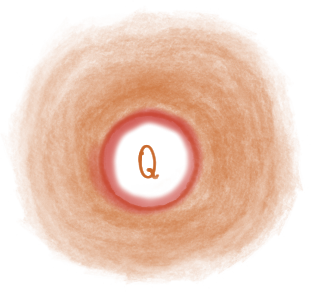
\includegraphics[width=0.4\textwidth]{field_concept.png}
    \caption{Concepto de campo eléctrico.}
    \label{fig:concepto_campo_electrico}
\end{figure}

En lugar de pensar que una carga actúa instantáneamente sobre otra, se puede imaginar que una carga genera algo en el espacio a su alrededor que luego interactúa con otras cargas. Este ``algo'' es el \textbf{campo eléctrico}. La idea es la siguiente:

\begin{enumerate}
    \item Una carga fuente \( Q \) modifica el espacio circundante.
    \item Cualquier otra carga \( q \) que se coloque en ese espacio experimentará una fuerza debido a esta modificación.
    \item Para cuantificar esa modificación, definimos el campo eléctrico como la \textbf{fuerza por unidad de carga de prueba}.
\end{enumerate}

\paragraph{Idea conceptual del campo eléctrico}

Si te preguntas qué es el campo eléctrico, puedes responder según la descripción previa: ``el campo eléctrico es una propiedad del espacio que rodea a una carga eléctrica capaz de interactuar con otras cargas''. Sin embargo la idea es entender qué significa que una carga eléctrica modifique las propiedades del espacio que la rodea. Veamos un ejemplo de esto para entenderlo mejor.

Supongamos que tengo una carga positiva (un protón) y quiero que se quede totalmente quieto. Entonces ¿Cómo podemos lograr esto? 
Bueno, pues es bastante sencillo. Buscamos alguna carga \( Q \) que a una distancia \( r \) haga que la carga \( q \) del protón anule las fuerzas que interactúan con la carga.

Supongamos que la única fuerza que está interactuando con el protón es la fuerza peso. Entonces tendriamos que encontrar cualquier combinación de \( Q \) y \( r \) que cumpla:

\[
    F_g = F_e = k_e \frac{Q \cdot q}{r^2}
\]

Como nuestras incógnitas son \( Q \) y \( r \) vamos a tener infinitas posibilidades que solucionan muestro problema. Pero antes de dar por terminado el problema te pregunto ¿Qué tienen en común todas las soluciones?

Todas las soluciones están ocacionando el mismo efecto en el protón, una fuerza vertical y hacia arriba (en sentido opuesto al peso). Podriamos expresar esto diciendo: ``todas las soluciones generan una perturbación identica en el punto del espacio donde se encuentra el protón''. O, en otras palabras, todas las soluciones generan un campo eléctrico de las mismas características en donde está el protón.

Es más, cualquier partícula que coloquemos en el lugar del protón, con cualquier carga, por ejemplo una partícula con tres veces la carga del protón pero negativa, sentirá una fuerza proporcional a la que sentía el protón. En el caso de este ejemlo sería una fuerza igual a tres veces el peso del protón en el mimo sentido al peso (por ser negativa).

\paragraph{Formulando el Campo Eléctrico}

El campo eléctrico \( \vec{E} \) se define como la fuerza por unidad de carga de prueba \textbf{positiva} en un punto en el espacio. Esto puede expresarse como:

\begin{equation}
    \vec{E} = \frac{F}{q^{+}} = k_e \frac{Q}{r^2}
\end{equation}

donde:
\begin{itemize}
    \item \( Q \) es la carga que genera el campo (puntual).
    \item \( r \) es la distancia entre la carga de prueba y \( Q \).
\end{itemize}

En caso de que exista más de una carga que genera el campo, se aplica \textbf{el principio de superposición} que consiste en sumar todos todos los campos vectorialmente.

\[
\vec{E} = \sum{\vec{E}_i} = k \cdot \sum{\frac{Q_i}{r^2_i}} \hat{r}_i
\]

Sin embargo, en muchos casos, tenemos una distribución continua de carga en vez de una colección de cargas discretas. En esta situación, la carga puede estar distribuida a lo largo de una recta, sobre alguna superficie, por todo un volumen. Siguiendo el concepto de superposición de cargas tendríamos:

\[
\vec{E} = k \lim_{\Delta q_i \to 0} \sum_i{\frac{\Delta q_i}{r_i^2}\hat{r}_i} = k \int \frac{dq}{r^2} \hat{r}
\]

En los casos que debemos calcular el campo de una distribución continua tendremos la \textit{densidad de carga}. Pero ¿Qué es la densidad de carga?

La \textbf{densidad de carga} es una \textit{medida de cuánta carga eléctrica hay distribuida} sobre una determinada región del espacio. Se utiliza cuando las cargas no están concentradas en puntos, sino \textbf{distribuidas} sobre líneas, superficies o volúmenes.

Dependiendo del tipo de distribución, hay tres formas principales:

\subparagraph{1. Densidad lineal de carga:}

Se usa cuando la carga está distribuida a lo largo de una línea (como un alambre).

\[
\lambda = \frac{Q}{l} ~ ~ \rightarrow ~ ~ dq = \lambda dl
\]

\begin{itemize}
    \item \( \lambda \): densidad lineal (C/m)  
    \item \( Q \): pequeña cantidad de carga  
    \item \( l \): pequeña longitud del alambre  
\end{itemize}

\subparagraph{2. Densidad superficial de carga:}

Se usa para cargas sobre una superficie (como una lámina metálica cargada).

\[
\sigma = \frac{Q}{A} ~ ~ \rightarrow ~ ~ dq = \sigma dA
\]

\begin{itemize}
    \item \( \sigma \): densidad superficial (C/m²)  
    \item \( Q \): carga sobre un área pequeña  
    \item \( A \): área considerada  
\end{itemize}

\subparagraph{3. Densidad volumétrica de carga:}

Se usa cuando la carga ocupa un volumen (como una nube de plasma).

\[
\rho = \frac{Q}{V} ~ ~ \rightarrow ~ ~ dq = \rho dV
\]

\begin{itemize}
    \item \( \rho \): densidad volumétrica (C/m³)  
    \item \( Q \): carga dentro de un pequeño volumen  
    \item \( V \): volumen correspondiente  
\end{itemize}


Estas densidades permiten convertir una distribución continua de carga en una integral, y así calcular el campo eléctrico o el potencial.  
Por ejemplo, si conocés \( \lambda(x) \), podés calcular el campo eléctrico de una varilla cargada mediante:

\[
\vec{E} = \frac{1}{4\pi\varepsilon_0} \int \frac{\lambda(x)\, dx}{r^2} \hat{r}
\]

\paragraph{Visualización del campo eléctrico}

Para visualizar el campo eléctrico veamos un ejemplo sencillo. Supongamos que tenemos tres cargas eléctricas de distinto valor ubicadas en tres lugares distintos. Todas estas cargas están fijas en su posición y no pueden moverse (ver figura \ref{fig:campo_electrico_ejemplo_1}). 

\begin{figure}[ht]
    \centering
    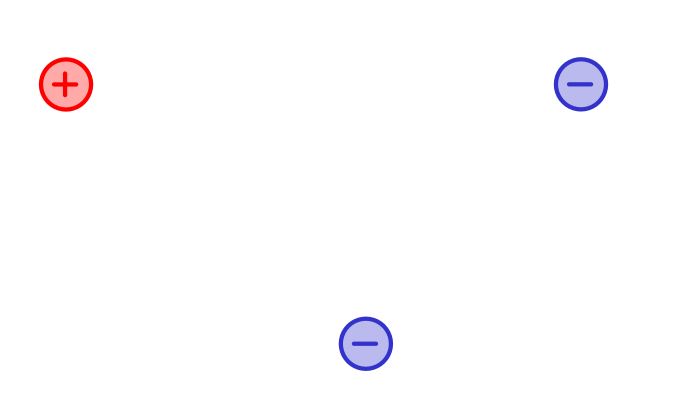
\includegraphics[width=0.5\textwidth]{field_ex_1.png}
    \caption{tres cargas fijas en el espacio.}
    \label{fig:campo_electrico_ejemplo_1}
\end{figure}

Estas tres cargas posicionadas en el espacio constituyen lo que llamaremos \textbf{carga fuente}. Estas tres cargas fuente son capaces de generar una fuerza en cualquier partícula con carga que se coloque en este espacio. Podemos decir entonces, que las tres cargas le dan una propiedad eléctrica al espacio que las rodea. A esta propiedad que adquiere el espacio por culpa de las cargas le llamaremos campo eléctrico y existe independientemente de que haya otra cuarta carga presente o no.

Ahora supongamos que queremos jugar con el campo generado, y tomamos una cuarta carga \( q^{+} \), en este caso la carga será positiva, y la llamaremos \textbf{carga de prueba}. Entonces colocamos la carga de prueba en el centro de las tres cargas y la soltamos (ver figura \ref{fig:campo_electrico_ejemplo_2})

Cuando la soltamos, la carga será empujada hacia algún lugar, ya que, experimentará una fuerza debido a la interacción con las otras cargas. Ya sabemos que las cargas del mismo signo se repelen y las de signo opuesto se atraen.

\begin{figure}[ht]
    \centering
    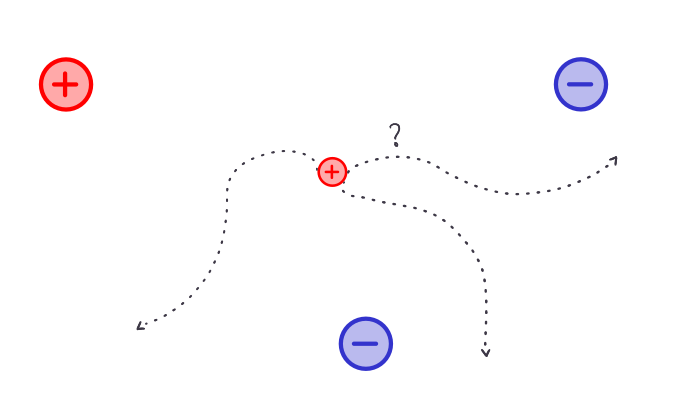
\includegraphics[width=0.5\textwidth]{field_ex_2.png}
    \caption{colocamos una cuarta carga en el centro y la soltamos.}
    \label{fig:campo_electrico_ejemplo_2}
\end{figure}

Entonces aquí tenemos tres cargas aplicando tres fuerzas distintas, ¿qué hacemos? Sumar todas las fuerzas. Algunas se van a contrarrestar un poco al estar en direcciones opuestas, pero otras se van reforzar al tirar en el mismo sentido.

La suma de todas estas fuerzas (fuerza resultante) nos indica hacia dónde va ir la carga y la intensidad del empujón que sentirá (magnitud de la fuerza). Si realizamos esto en cada punto del espacio acabaríamos llenando el espacio de vectores de fuerza, esto se vería como un ``mapa de flechas'' que representan la fuerza que siente la carga de prueba en cada punto.

\textbf{Pero espera:} imaginemos que realizamos todos los cálculos con una carga de prueba de \( 1 \si{\coulomb} \). Y esa carga de prueba en realidad solo la usamos para realizar los cálculos del mapa, pero en realidad no existe. Entonces este mapa lo podemos usar para saber qué fuerza sentiría una carga \( q \) cualquiera.
Seguro te preguntarás ¿Cómo es eso? Es bien sencillo, presta atención a lo siguiente. Si recordamos la ecuación de la fuerza debido a la interacción entre cargas tenemos:

\[
\vec{F}_e = k\frac{Q\cdot q^{+}}{r^2}\hat{r} 
\]

Ahora, recordando que \( Q \) era nuestra carga fuente (formada por las tres cargas) y \( q^{+} \) nuestra carga de prueba de \( 1 \si{\coulomb} \) que usamos para hacer todas las cuentas, si quitamos la carga de prueba, como en la ecuación de fuerza es un factor neutro (multiplica por 1), el resultado no cambiaría cuantitativamente, sin embargo cambiarían las unidades. Veamos como queda:

\[
\vec{F}_e ~ [\si{\newton}] \neq k \frac{Q}{r^2} \hat{r} ~ [\si{\newton\per\coulomb}]
\]

Vemos que lo que resulta es una desigualdad, ya que las unidades no coinciden. Si bien numericamente es lo mismo, dimensionamente no. Para arreglar este problema entonces, en vez de quitar directamente la carga, podemos dividir ambos miembros por \( q^{+} \), y no romperíamos las unidades:

\[
\frac{\vec{F}_e}{q^{+}} ~ [\si{\newton\per\coulomb}] = k \frac{Q}{r^2} \hat{r} ~ [\si{\newton\per\coulomb}]
\]

\begin{figure}[ht]
    \centering
    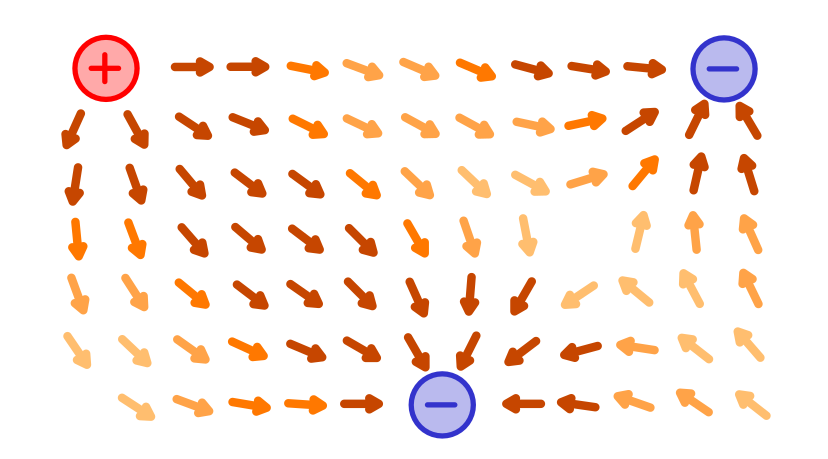
\includegraphics[width=0.5\textwidth]{field_example.png}
    \caption{mapa de la fuerza que siente \(q^{+}\) en cada punto.}
    \label{fig:campo_electrico_ejemplo_3}
\end{figure}

¿Qué nos dice este ``mapa de flechas''? Este mapa de flechas nos dice la \hl{fuerza por unidad de carga} que generan las cargas fuente. Es decir, si colocamos una carga unidad (como \(q^{+}\)), entonces la relación es \(1:1\), pero podemos colocar cualquier carga \(q\) y multiplicarla por el campo.

\begin{equation}
    \vec{E} = \frac{\vec{F}}{q^{+}}
    \label{eq:campo_electrico}
\end{equation}

donde:
\begin{itemize}
    \item \( \vec{E} \) es el campo eléctrico en ese punto,
    \item \( \vec{F} \) es la fuerza experimentada por la carga de prueba \( q^{+} \),
    \item \( q^{+} \) es la carga de prueba.
\end{itemize}

Ahora, como vimos, la carga de prueba es una carga hipotética utilizada para medir el campo sin modificarlo. Como la carga de prueba es positiva, entonces vemos que una carga fuente \(Q\) cualquiera, respeta la siguiente distribución: si la carga \(Q\) es \textbf{negativa}, las líneas de campo son entrantes, si la carga \(Q\) es \textbf{positiva}, las líneas de campo son salientes:

\begin{figure}[ht]
    \centering
    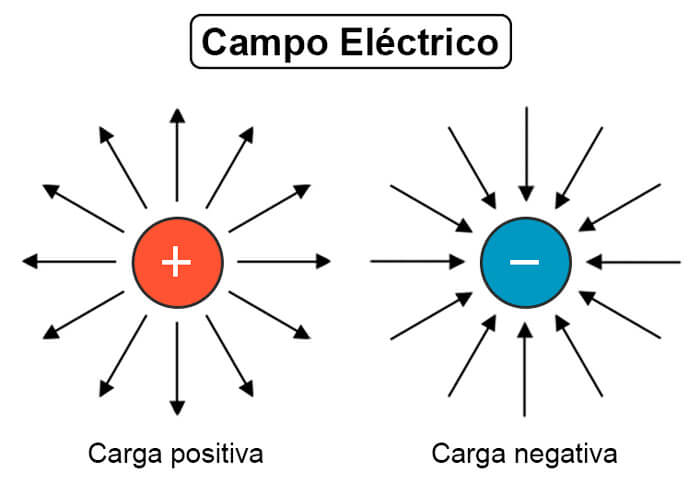
\includegraphics[width=0.5\textwidth]{electric_field.jpg}
    \caption{Campo eléctrico de una carga puntual positiva y una negativa.}
    \label{fig:campo_electrico}
\end{figure}

Este resultado nos dice que el \hl{campo eléctrico} \textbf{se aleja} de cargas positivas y \textbf{se dirige hacia} cargas negativas. Además disminuye con el cuadrado de la distancia y es una propiedad del espacio ya no depende de la carga de prueba \( q \), sino solo de \( Q \).

Es muy importante tener en cuenta las premisas usadas para formular el \textbf{campo eléctrico}:
\begin{itemize}
    \item \textit{La carga fuente modifica el espacio circundante:} El campo eléctrico es una propiedad del espacio y es generado por una carga fuente.
    \item \textit{El campo es independiente de la carga de prueba:} La carga de prueba se usa solo como herramienta de medición.
    \item \textit{El campo es un campo vectorial:} Tiene dirección y magnitud en cada punto del espacio.
    \item \textit{El campo sigue el principio de superposición:} Si hay varias cargas, el campo total en un punto es la suma vectorial de los campos generados por cada una.
    \item \textit{La carga de prueba es positiva:} Para determinar el sentido del campo es importante tener en cuenta que la carga de prueba es positiva, esto permite ver con claridad cuando el campo es entrante o saliente para una carga puntual, o poder predecir correctamente el sentido del campo en una distribución de cargas (ya sea discreta o continua).
\end{itemize}

\subsubsection{Lineas de campo eléctrico}

Las líneas de campo no son más que un medio para visualizar el patrón formado por el campo eléctrico a través del trazo de líneas conocidas como \textbf{líneas de campo eléctrico}. Estas líneas relacionan el campo eléctrico con una región del espacio de la siguiente manera:
\begin{itemize}
    \item El vector \(\vec{E}\) del campo eléctrico es tangente a la línea del campo eléctrico en cada punto y la dirección de la linea de campo es igual a la del campo eléctrico.
    \item El número de líneas de campo que pasan por una superficie perpendicular a dichas líneas es proporcional a la magnitud de campo.
\end{itemize}

\begin{figure}[ht]
    \centering
    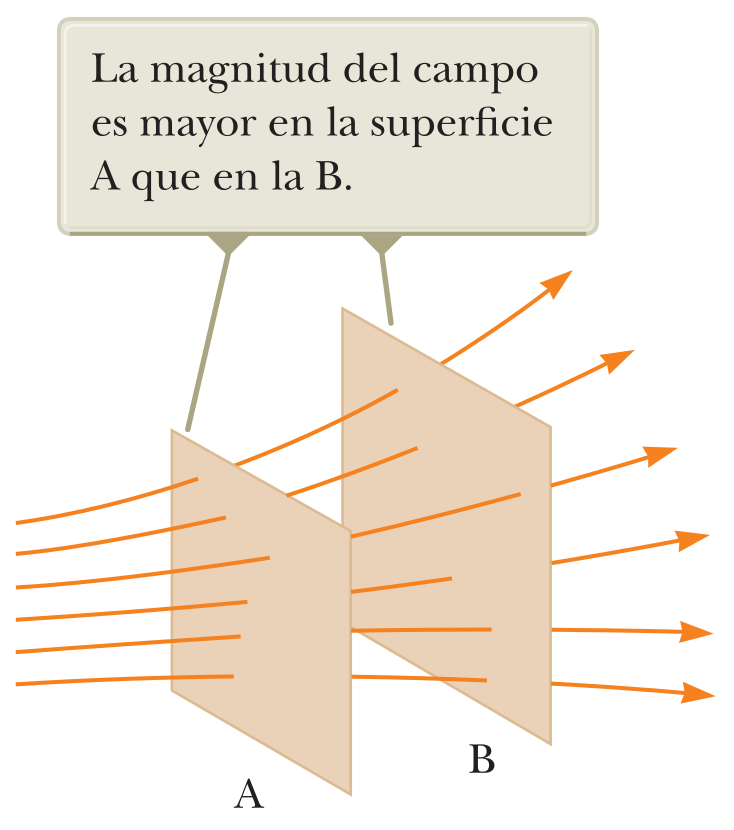
\includegraphics[width=0.5\textwidth]{field-lines.png}
    \caption{Líneas de campo eléctrico que atraviesan dos superficies}
    \label{fig:lineas_de_campo}
\end{figure}

Pongamos este concepto en palabras simples ¿Recuerdas el ejemplo de las tres cargas y el ``mapa de flechas''? Bueno, las líneas de campo nos ayudan a visualizar el ``mapa de flechas'' de una forma más cómoda.

\begin{figure}[ht]
    \centering
    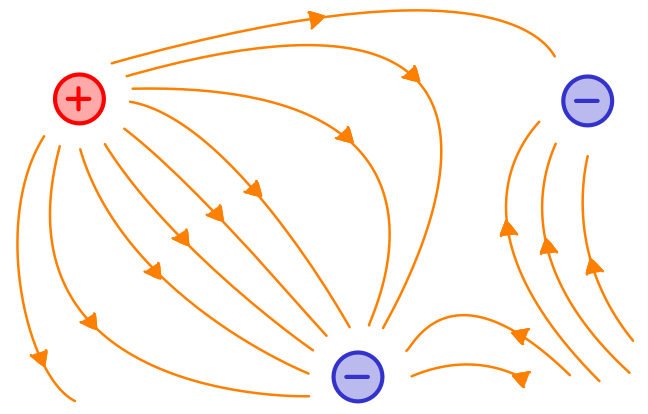
\includegraphics[width=0.4\textwidth]{field_lines_ex.png}
    \caption{Ejemplo del ``mapa de flechas'' visualizado con líneas de campo}
    \label{fig:ej_lineas_de_campo}
\end{figure}

En este caso se puede ver que las líneas de campo están más juntas cuando nos acercamos a las cargas, y se van separando cuando nos alejamos. La proximidad entre líneas de campo nos indica que el campo es intenso. Si las líneas están distantes entre sí indica que el campo es menos intenso. Esto se puede verificar con la ecuación del campo eléctrico, ya que el campo disminuye con el cuadrado de la distancia. Esto significa que según más nos alejamos de las cargas fuente, el campo disminuye.

\subsection{Flujo eléctrico}

\subsection{Flujo eléctrico}
\label{sec:flujo_electrico}

Hasta ahora hemos visto una idea general de las líneas de campo eléctrico. Es decir, vimos una explicación que busca dar una idea general de cómo funcionan las líneas de campo eléctrico, su forma, su dirección y su relación con las cargas, pero sin proporcionar fórmulas o cantidades específicas. En este apartado, vamos a explicar con mayor formalidad este concepto, donde se considerará la magnitud del campo eléctrico y el área a través de la cual se mide el flujo eléctrico, utilizando la relación matemática entre estas variables.

\subsubsection{Definición}

El \hl{flujo eléctrico} es una medida de la cantidad de campo eléctrico que atraviesa una superficie dada. Se define matemáticamente como el producto de la magnitud del campo eléctrico (\(E\)) y el área (\(A\)) de la superficie a través de la cual se mide el flujo, así como el coseno del ángulo (\(\theta\)) entre la dirección del campo eléctrico y la normal (perpendicular) a la superficie. La fórmula para calcular el flujo eléctrico (\(\Phi_E\)) es:

\begin{figure}[ht]
    \centering
    \begin{subfigure}[b]{0.45\textwidth}
        \centering
        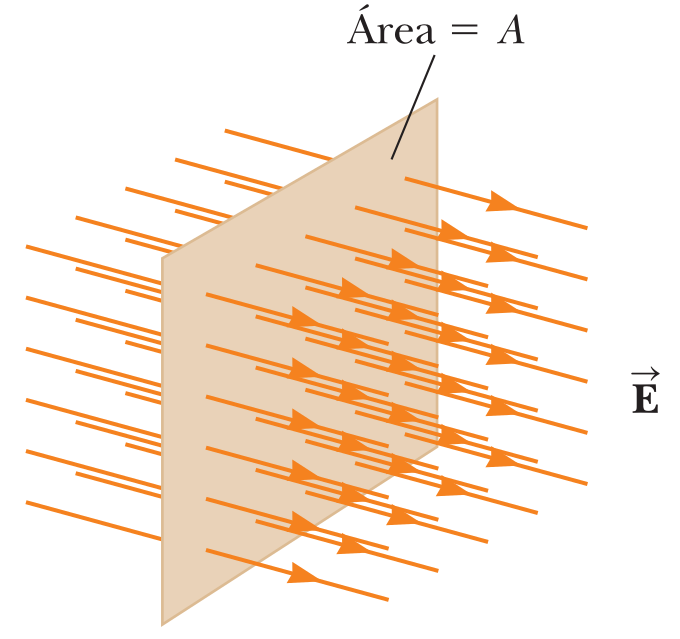
\includegraphics[width=\textwidth]{flujo_1.png}
        \caption{flujo sobre un area perpendicular.}
        \label{fig:flujo1}
    \end{subfigure}
    \hfill
    \begin{subfigure}[b]{0.45\textwidth}
        \centering
        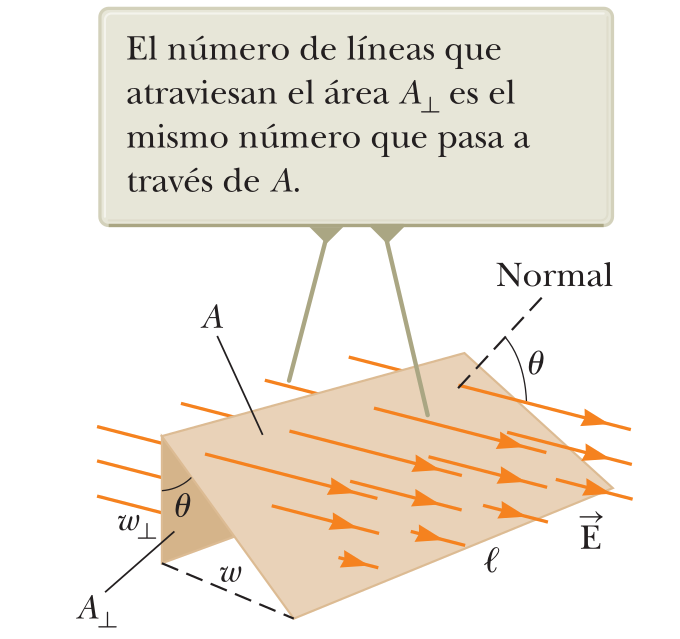
\includegraphics[width=\textwidth]{flujo_2.png}
        \caption{flujo sobre un area inclinada.}
        \label{fig:flujo2}
    \end{subfigure}
    \caption{Flujo eléctrico}
    \label{fig:flujo eléctrico}
\end{figure}

\[
\Phi_E = E \cdot A \cdot \cos(\theta)  ~~ \left[\frac{\si{\newton \meter \squared}}{\si{\coulomb}}\right]
\]

Donde:
\begin{itemize}
    \item \(\Phi_E\) es el flujo eléctrico.
    \item \(E\) es la magnitud del campo eléctrico.
    \item \(A\) es el área de la superficie.
    \item \(\theta\) es el ángulo entre la dirección del campo eléctrico y la normal a la superficie.
\end{itemize}

Otra forma más general de escribir el flujo eléctrico es usando el \hl{producto escalar}. Para poder usar el producto escalar, necesitamos dos vectores, y en este caso solo tenemos el vector de campo. Entonce podemos definir un vector normal a la superficie con igual magnitud al área de la superficie. Entonces el producto escalar entre el vector campo eléctrico (\(\vec{E}\)) y el vector normal al area \(\vec{A}\) es:

\begin{equation}
    \Phi_E = \vec{E} \cdot \vec{A} = E A \cos \theta
    \label{eq:flujo_electrico}
\end{equation}

Hay que tener muy presente que \(\Phi_E\) es un \textbf{ESCALAR} no un vector. Y otro factor a considerar es que la ecuación \eqref{eq:flujo_electrico} solo se puede usar si el campo \(\vec{E}\) es constante. Sin embargo, en general, el campo \(\vec{E}\) no suele ser constante, entonces una forma de conseguir el flujo eléctrico total en una superficie \(S\) donde el campo no es constante es sumando todas las pequeñas contribuciones de flujo eléctrico en pequeñas porciones de area (\(dA\)), resultando en la siguiente integral:

\begin{equation}
    \Phi_E = \int_{S} \vec{E} \cdot d\vec{A}
    \label{eq:flujo_electrico_integral}
\end{equation}

\subsubsection{Ley de Gauss}
\label{sec:ley_de_gauss}

El flujo eléctrico es importante en el estudio del electromagnetismo porque está relacionado con la ley de Gauss, que establece que el flujo eléctrico a través de una superficie \textbf{cerrada} (con frecuencia llamada \textit{superficie gaussiana}) es proporcional a la carga eléctrica total encerrada dentro de esa superficie. Suponga una carga puntual positiva \(q\) ubicada en el centro de una esfera de radio \(r\) como se observa en la figura \ref{fig:superficie_gaussiana}.

\begin{wrapfigure}{r}{0.35\textwidth}
    \centering
    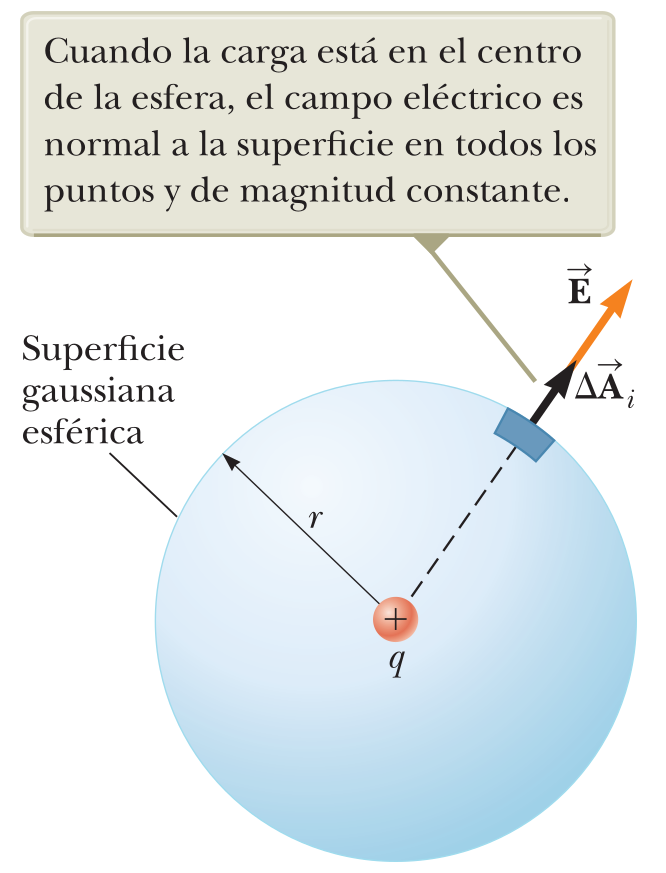
\includegraphics[width=\linewidth]{ley_de_gauss.png}
    \caption{Superficie gaussiana esférica de radio \(r\) que rodea una carga puntual \(q\).}
    \label{fig:superficie_gaussiana}
\end{wrapfigure}
De la ecuación de campo eléctrico \eqref{eq:campo_electrico}, se sabe que la magnitud del campo eléctrico sobre todos los puntos de la superficie (\(S\)) de la esfera es \(\vec{E} = k q/r^2\). Las líneas de campo están dirigidas radialmente hacia afuera y por tanto son perpendiculares a la superficie en todos sus puntos. Es decir, en cada punto de la superficie, \(\vec{E}\) es paralelo al vector \(d\vec{A}\) que representa un elemento de área muy pequeño que rodea al punto en la superficie. Por lo tanto, el flujo neto a través de la superficie gaussiana es igual a:

\begin{align*}
    \Phi_E =& \oint_S \vec{E} \cdot d\vec{A} \\
            =& \oint_S E \cos(0) ~ dA \\
            =& \oint_S E ~ dA \\
    \Phi_E =& E ~ \oint_S dA
\end{align*}
aquí tenemos que \(E=kq/r^2\) donde \(r\) es conocido y vale el radio de la esfera, \(q\) es el valor de la carga en el centro de la esfera y \(k = 1/4\pi\epsilon_0\). Luego la integral resulta en la superficie de una esfera que es \(4\pi r^2\). Entonces:

\[
\Phi_E = E ~ \oint_S dA = \frac{q}{4\pi \epsilon_0 r^2} \cdot 4\pi r^2 = \boxed{\frac{q}{\epsilon_0}} 
\]

Este resultado dice muchas cosas:
\begin{itemize}
    \item \textbf{Primero}: el flujo eléctrico \(\Phi_E\) no depende del radio de la superficie esférica.
    \item \textbf{Segundo}: el flujo es directamente proporcional a la carga encerrada en el interior de la superficie gaussiana.
    \item \textbf{Tercero}: el flujo es inversamente proporcional al valor de \(\epsilon\), en el ejemplo se trabajó con vacío, pero puede ser cualquier material no conductor con otro valor de \(\epsilon\).
\end{itemize}

En base a esto podemos sacar una conclusión, supongamos ahora que la superficie no es esférica ¿El flujo será el mismo que el de la esfera? Bueno, pues voy a hacer un adelanto, si lo es, pero ¿Por qué? Pensemos en la definición de flujo, sea cualquier superficie que rodea la esfera, el flujo será igual a el \(\vec{E}\cdot d\vec{A}\). Como vimos anteriormente esto representa la cantidad de líneas de campo que pasan por una superficie determinada. Como la superficie encierra la misma carga entonces saldrán la misma cantidad de líneas de campo por la superficie.

En este punto tal vez te preguntes ¿Cómo puede ser que no dependa del radio de la esfera, o mejor del tamaño de la superficie arbitraria cerrada? Es sencillo, si el tamaño de la superficie cerrada aumenta, entonces la distancia a la carga encerrada también aumentará, esto significa que la intensidad del campo disminuirá, entonces pasarán menos líneas de campo por cada \(dA\), pero como la superficie total a aumentado, entonces compensará la pérdida de intensidad del campo.

Con esto podemos armar una conclusión:

\begin{tcolorbox}[myconclusion]
    el flujo neto a través de \textit{cualquier} superficie cerrada que rodea a una carga puntual \(q\) está dado por \(q/\epsilon_0\) y es independiente de la forma de la superficie.
\end{tcolorbox}

Entonces, si suponemos varias superficies, llamemos \(S1\), \(S2\) y \(S3\) a las superficies que rodean la carga \(q\) (ver figura \ref{fig:superficie_gaussiana_arbitraria}). Todas estas superficies tienen el mismo flujo eléctrico, ya que todas encierran la misma carga \(q\). Se puede ver que el flujo neto es el mismo para todas las superficies.

\begin{figure}[ht]
    \centering
    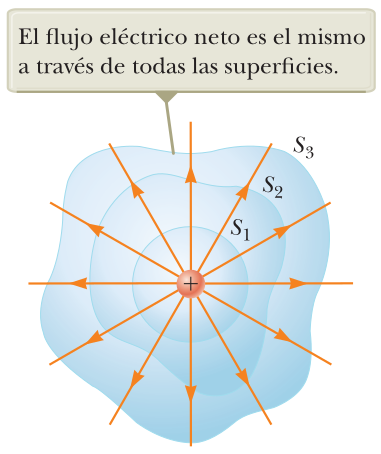
\includegraphics[width=0.35\textwidth]{flujo_neto.png}
    \caption{Distintas superficies gaussianas de forma arbitraria que rodean una carga puntual \(q\).}
    \label{fig:superficie_gaussiana_arbitraria}
\end{figure}

Por otro lado, si la carga \(q\) está fuera de la superficie gaussiana entonces la misma cantidad de líneas de campo que entran por un lado de la superficie, salen por el otro lado. Por lo tanto, el flujo neto a través de la superficie es cero. Esto se puede ver en la figura \ref{fig:flujo_neto_2} donde se observa que el flujo neto es cero.

\begin{figure}[ht]
    \centering
    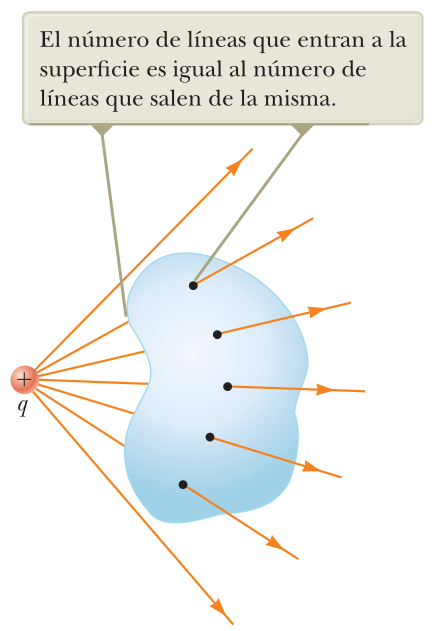
\includegraphics[width=0.4\textwidth]{flujo_neto_externo.png}
    \caption{Una carga puntual \(q\) fuera de la superficie.}
    \label{fig:flujo_neto_2}
\end{figure}

La forma matemática de ley de Gauss, es una generalización de lo anterior y establece que el flujo neto a través de cualquier superficie cerrada es

\begin{equation}
    \Phi_E = \oint_{S} \vec{E} \cdot d\vec{A} = \frac{q_{\text{int}}}{\varepsilon_0} ~~ \left[\frac{\si{\newton \meter \squared}}{\si{\coulomb}}\right]
\end{equation}
donde:
\begin{itemize}
    \item \( \Phi_E \) es el flujo de campo eléctrico a través de una superficie cerrada.
    \item \(E\) es el campo eléctrico en cada punto de esa superficie.
    \item \(dA\) es un vector diferencial de área que apunta hacia afuera de la superficie.
    \item \(q_{int}\) es la carga total encerrada dentro de la superficie.
    \item \(\epsilon_0\) es la permitividad del vacío, una constante del medio.
\end{itemize}

\begin{tcolorbox}[mydanger]
    CUIDADO: \(\vec{E}\) representa el campo eléctrico total, que incluye contribuciones de ambas cargas tanto del interior como del exterior de la superficie.    
\end{tcolorbox}

\paragraph{¿Qué nos dice esta ley, en términos simples?}

El flujo eléctrico representa la cantidad de ``líneas de campo eléctrico'' que atraviesan una superficie. La ley de Gauss nos habla de superficies cerradas, y nos dice que si hay carga dentro de una superficie cerrada, el campo eléctrico ``sale'' (o ``entra'') por esa superficie, generando un flujo distinto de cero. Si no hay carga neta dentro, el flujo eléctrico total es cero, aunque el campo pueda no ser nulo en todos los puntos. No importa la forma de la superficie, solo importa cuánta carga encierra, no cómo se distribuye el campo en detalle.

\subparagraph{¿Por qué es útil la ley de Gauss?}

La ley de Gauss es útil porque, en situaciones con alta simetría (esférica, cilíndrica, planar), permite calcular el campo eléctrico sin integrar la ley de Coulomb, por ejemplo:
\begin{itemize}
    \item Una esfera cargada uniformemente
    \item Un hilo infinitamente largo con carga lineal uniforme
    \item Un plano infinito cargado
\end{itemize}

\subparagraph{Ejemplo clásico: esfera cargada}

Supón una carga distribuida uniformemente en una esfera. Si elegimos una superficie esférica de radio  mayor al de la esfera, por simetría:
\[
\vec{E} = \text{constante} \quad \text{y} \quad \vec{E} \parallel d\vec{A}
\]
Entonces la integral se simplifica:
\[
\oint \vec{E} \cdot d\vec{A} = E \oint dA = E(4\pi r^2)
\]
Y por la ley de Gauss:
\[
E(4\pi r^2) = \frac{Q}{\varepsilon_0} \quad \Rightarrow \quad E = \frac{1}{4\pi\varepsilon_0} \frac{Q}{r^2}
\]
¡Y así recuperamos la fórmula del campo eléctrico de una carga puntual!

\subsection{Potencial eléctrico}

\subsection{Potencial eléctrico}

Cuando se coloca una carga \(q\) en un campo eléctrico \(\vec{E}\), la carga experimenta una fuerza \(\vec{F}=q\vec{E}\). Esta fuerza es conservativa, lo que significa que el trabajo realizado por la fuerza al mover la carga entre dos puntos \(A\) y \(B\) no depende de la trayectoria seguida, sino solo de los puntos inicial y final.

El trabajo realizado por la fuerza al mover la carga \(q\) desde el punto \(A\) hasta el punto \(B\) se define como:
\begin{equation*}
    W_{AB} = \int_A^B \vec{F} \cdot d\vec{s} = \int_A^B q\vec{E} \cdot d\vec{s}
\end{equation*}
donde \(d\vec{s}\) es un elemento diferencial de desplazamiento a lo largo de la trayectoria. Y como la fuerza eléctrica es conservativa, podemos expresarla en términos de la energía potencial eléctrica \(U\):
\begin{equation*}
    W_{AB} = U_A - U_B = -\Delta U
\end{equation*}

\subsubsection{Definición de potencial eléctrico}

Para una posición conocida de la carga de prueba en el campo, el sistema carga-campo tiene una energía potencial \(U\) relativa a la configuración del sistema definida como \(U=0\). Al dividir la energía potencial entre la carga de prueba \(q\), obtenemos el \textbf{potencial eléctrico} \(V\) en un punto \(P\) del campo eléctrico:

\begin{equation}
    V = \frac{U}{q}
    \label{eq:potential}
\end{equation}

El potencial eléctrico es una magnitud escalar que se mide en \(\text{V}\) (voltios) y se define como la energía potencial por unidad de carga.

Teniendo en cuenta la definición de potencial (ecuación \eqref{eq:potential}) la \textbf{diferencia de potencial} \(\Delta V = V_B - V_A\) entre dos puntos \(A\) y \(B\) en un campo eléctrico se define como el cambio en energía potencial por unidad de carga al mover una carga de prueba \(q\) entre esos dos puntos:

\begin{equation}
    \Delta V = \frac{\Delta U}{q} = -\int_A^B \vec{E} \cdot d\vec{s}
    \label{eq:potential_difference}
\end{equation}

Por la ecuación \eqref{eq:potential_difference}, el trabajo realizado por un agente externo al desplazar una carga \(q\) a través de un campo eléctrico con una velocidad constante es:

\[
W=q\Delta V
\]

Es muy importante que el desplazamiento de la carga \(q\) sea a velocidad constante, ya que si no lo es, el trabajo realizado por el agente externo no será igual al trabajo realizado por la fuerza eléctrica. 

Nótese que el concepto de potencial eléctrico se concive de forma similar al de campo eléctrico. Se usa una carga de prueba positiva \(q\) haciendo que sólo dependa de la carga fuente \(Q\) que genera el campo eléctrico. 

\subsubsection{Diferencia de potencial en un campo eléctrico uniforme}

La ecuación \eqref{eq:potential_difference} es válida en todos los campos eléctricos, sean uniformes o no. En un campo eléctrico uniforme, la magnitud del campo \(\vec{E}\) es constante y la dirección de \(\vec{E}\) es la misma en todos los puntos del campo. En este caso, la diferencia de potencial entre dos puntos \(A\) y \(B\) separados por una distancia \(d\) en la dirección del campo eléctrico se puede expresar como:
\begin{equation}
    \Delta V = -\int_A^B \vec{E} \cdot d\vec{s} = -E \, \int_A^B ds = \boxed{-Ed}
    \label{eq:potential_uniform}
\end{equation}
donde \(E\) es la magnitud del campo eléctrico y \(d\) es la distancia entre los puntos \(A\) y \(B\) en la dirección del campo.

El signo negativo indica que el potencial en el punto \(B\) es menor que el potencial en el punto \(A\) si la carga de prueba se mueve en la dirección del campo eléctrico. Esto significa que el trabajo realizado por la fuerza eléctrica es negativo, lo que implica que la energía potencial disminuye al mover la carga en la dirección del campo eléctrico.

\begin{figure}[ht]
    \centering
    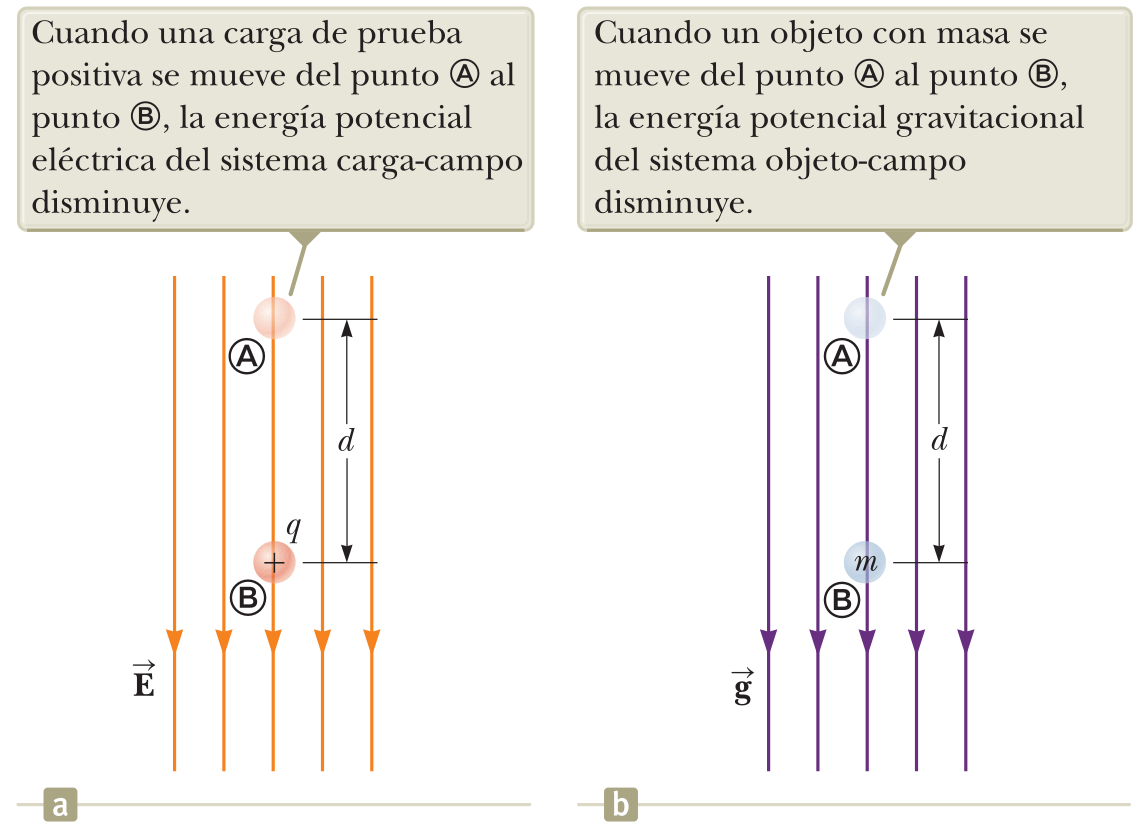
\includegraphics[width=1\textwidth]{potential_const_field.png}
    \caption{Comparación de la energía potencial eléctrica y gravitatoria.}
    \label{fig:potential_uniform}
\end{figure}

\begin{tcolorbox}[mydanger]
    CUIDADO: si la carga \(q\) es negativa, la situación se invierte. El sistema gana energía potencial al mover la carga \(q\) en la dirección del campo eléctrico, y disminuye al moverla en la dirección opuesta.    
\end{tcolorbox}

\subsubsection{Potencial eléctrico debido a una carga puntual}

\begin{wrapfigure}{l}{0.32\textwidth}
    \centering
    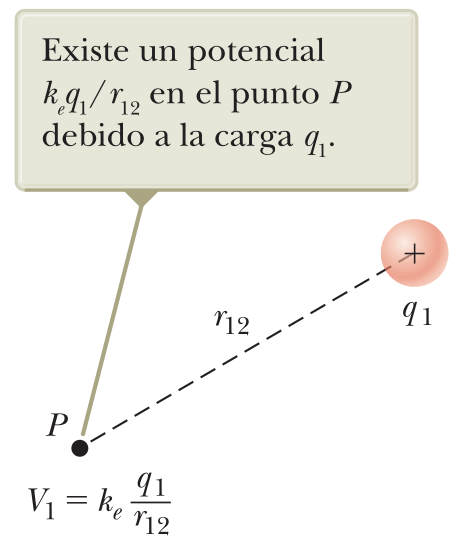
\includegraphics[width=\linewidth]{puntual_potential_1.png}
    \caption{Potencial en el punto \(P\) debido a \(q_1\).}
    \label{fig:potential_point_charge}
\end{wrapfigure}

Como se menciona en la definición, la energía potencial es relativa al punto que se ha definido como ``0''. Con  el potencial eléctrico pasa lo mismo, entonces si queremos saber el potencial en un punto \(P\) del campo eléctrico, sabemos que es igual al trabajo realizado por la fuerza eléctrica al mover una carga de prueba \(q\), pero ¿Desde donde hasta donde? Bueno, podemos definir que nuestro potencial sea cero cuando la carga \(q\) esté infinitamente alejada de la fuente. Entonces el potencial en el punto \(P\) es trabajo para mover la carga de prueba desde el infinito hasta el punto \(P\):

\begin{align*}
    V_P &= - \lim_{a \to \infty}\int_{a}^P \vec{E} \cdot d\vec{r}\\
        &= - \lim_{a \to \infty}\int_{a}^P \frac{kq_1}{r^2} \cdot dr\\
        &= -kq_1 \, \lim_{a \to \infty} \int_{a}^P \frac{1}{r^2} \cdot dr\\
        &= -kq_1 \, \lim_{a \to \infty} \left[ -\frac{1}{r} \right]_{a}^P\\
        &= -kq_1 \, \lim_{a \to \infty} \left[ -\frac{1}{P} + \frac{1}{a} \right]\\
        &= -kq_1 \, \left[ -\frac{1}{P} + 0 \right] \\
    V_P &= k\frac{q_1}{r_{12}} = \lVert\vec{E}\rVert \, \lVert\vec{r}_{12}\rVert \cos(0)
\end{align*}
por ser \(\vec{E}\) y \(\vec{r}_{12}\) paralelos. Entonces el potencial eléctrico en un punto \(P\) debido a una carga puntual \(q_1\) es:
\begin{equation}
    \boxed{V_P = k\frac{q_1}{r_{12}} = E \, r_{12}}
    \label{eq:potential_point_charge}
\end{equation}
donde \(q_1\) es la carga fuente, \(E\) el campo generado por \(q_1\) y \(r_{12}\) la distancia a un punto en el campo eléctrico.

El potencial eléctrico debido a múltiples cargas puntuales se basa en el principio de superposición, que establece que el potencial eléctrico total en un punto es igual a la suma algebraica de los potenciales individuales producidos por cada carga.

\begin{equation}
    V_{total} = \sum_{i=1}^{n} V_i = k \sum_{i=1}^{n} \frac{q_i}{r_i}
\end{equation}

\subsubsection{Obtención de \texorpdfstring{\(\vec{E}\)}{E} a partir de \texorpdfstring{\(V\)}{V}}

El campo eléctrico \(\vec{E}\) y el potencial eléctrico \(V\) están relacionados, como se muestra en la ecuación \eqref{eq:potential_point_charge}, que se usa para encontrar \(V\) en un punto cuando se conoce \(\vec{E}\). Sin embargo, también podemos encontrar \(\vec{E}\) a partir de \(V\) usando la relación:

\begin{equation}
    dV = -\vec{E} \cdot d\vec{s}
    \label{eq:field_from_potential_differential}
\end{equation}
y si estamos trabajando con una única coordenada podemos escribir la ecuación \eqref{eq:field_from_potential_differential} como:

\[
    dV = -E \, ds \quad \Rightarrow \quad E = -\frac{dV}{ds}
\]

Sin embargo, en general, el potencial eléctrico es una función de las tres coordenadas espaciales. Si \(V(r)\) se da en coordenadas cartesianas, las componentes \((E_x, E_y, E_z)\) del campo eléctrico pueden ser determinadas fácilmente a partir de \(V(x, y, z)\) como derivadas parciales

\begin{equation}
    \vec{E} = -\nabla V
    \label{eq:field_from_potential}
\end{equation}
donde \(\nabla\) es el operador nabla, que representa el \hl{gradiente del potencial eléctrico}. Esta relación indica que el campo eléctrico es igual al negativo del gradiente del potencial eléctrico. En otras palabras, el campo eléctrico apunta en la dirección de mayor disminución del potencial eléctrico.

\paragraph{Recordatorio: operador nabla}

El operador \textbf{nabla} (\(\nabla\)), también conocido como \textbf{operador del gradiente}, es una herramienta matemática usada en cálculo vectorial y análisis multivariable. Se utiliza para representar derivadas en múltiples dimensiones.

Formalmente, el operador nabla se define como:

\[
\nabla = \left( \frac{\partial}{\partial x}, \frac{\partial}{\partial y}, \frac{\partial}{\partial z} \right)
\]

Es un operador vectorial que, aplicado a diferentes tipos de funciones, da lugar a distintos conceptos. En nuestro caso solo vamos a repasar el concepto de gradiente.

Cuando se aplica el operador nabla a una función escalar \( f(x, y, z) \), produce un \textbf{campo vectorial} que apunta en la dirección de mayor incremento de la función. Se expresa como:

\[
\nabla f = \left( \frac{\partial f}{\partial x}, \frac{\partial f}{\partial y}, \frac{\partial f}{\partial z} \right)
\]

Este vector resultante indica la dirección en la que la función crece más rápidamente y su magnitud corresponde a la tasa de cambio máxima. En el caso de \(\vec{E}\) y \(V\), \(\vec{E}\) es el gradiente de \(V\) representa una función vectorial que apunta en la dirección de mayor aumento del potencial eléctrico.

\subsection{Capacitores}

Un \textbf{capacitor}, también conocido como \textbf{condensador}, es un componente eléctrico pasivo que tiene la capacidad de \textbf{almacenar energía en forma de un campo eléctrico}. Está compuesto por dos conductores (llamados placas) separados por un material dieléctrico, que actúa como aislante.

Cuando se aplica una diferencia de potencial (voltaje) entre las placas, una de ellas acumula carga positiva y la otra carga negativa, generando así un campo eléctrico entre ellas. La capacidad del capacitor para almacenar carga depende de sus características físicas y del dieléctrico utilizado.

La \textbf{capacitancia} es una medida de esa capacidad de almacenamiento de carga eléctrica. Se define como:

\begin{equation}
    C = \frac{Q}{V}
    \label{eq:capacitance}    
\end{equation}

donde:

\begin{itemize}
    \item \( C \) es la \textbf{capacitancia} del capacitor, medida en faradios (\(\si{\farad}\)).
    \item \( Q \) es la \textbf{carga eléctrica} almacenada en el capacitor, medida en coulombs (\(\si{\coulomb}\)).
    \item \( V \) es la \textbf{diferencia de potencial} entre las placas del capacitor, medida en voltios (\(\si{\volt}\)).
\end{itemize}

Un faradio es una unidad muy grande, por lo que en la práctica suelen utilizarse submúltiplos como el microfaradio (\(\mu\si{farad}\)), nanofaradio (n\(\si{\farad}\)) o picofaradio (p\(\si{\farad}\)).

La capacitancia depende de factores. Si se tienen placas paralelas de depende de factores como el área de las placas (\(A\)), la distancia entre ellas (\(d\)) y la permitividad del dieléctrico (\( \varepsilon \)) según la siguiente fórmula:

\[
C = \varepsilon \frac{A}{d}
\]

Este comportamiento hace que los capacitores sean ampliamente utilizados en circuitos electrónicos para funciones como almacenamiento de energía, filtrado, acoplamiento y desacoplamiento de señales, entre otras.

\subsubsection{Geometría de los conductores}

Cuando la \hl{geometría de los conductores} es distinta a la de un capacitor de placas planas y paralelas, la expresión de la capacitancia cambia, aunque el principio físico fundamental sigue siendo el mismo: almacenar energía en forma de campo eléctrico entre conductores separados por un dieléctrico.

En general, la \hl{capacitancia depende de la geometría de los conductores y del medio dieléctrico entre ellos}. A continuación, se presentan algunos casos comunes:

\paragraph{1. Capacitor esférico}

Consiste en dos esferas concéntricas de radios \( R_1 \) (interna) y \( R_2 \) (externa). Su capacitancia es:

\[
C = 4\pi \varepsilon_0 \varepsilon_r \frac{R_1 R_2}{R_2 - R_1}
\]

\paragraph{2. Capacitor cilíndrico}

Está formado por dos cilindros coaxiales, uno de radio interno \( a \) y otro de radio externo \( b \), y de longitud \( L \) (suponiendo \( L \gg b \)). La capacitancia es:

\[
C = \frac{2\pi \varepsilon_0 \varepsilon_r L}{\ln(b/a)}
\]

\paragraph{3. Geometrías irregulares o generales}

En geometrías más complejas, la capacitancia no puede obtenerse de forma analítica sencilla. En estos casos se recurre a:

\begin{itemize}
    \item Métodos numéricos
    \item Aproximaciones analíticas
    \item Medición experimental
\end{itemize}

Cuando se cambia la geometría, ya no es válida la fórmula simple \( C = \varepsilon \frac{A}{d} \). Es necesario **considerar la distribución del campo eléctrico** que surge de la nueva disposición geométrica, y calcular la capacitancia a partir de las definiciones fundamentales, como:

\[
C = \frac{Q}{V}
\]

donde \( V \) ahora debe calcularse usando la ley de Gauss o integrando el campo eléctrico apropiado para la geometría dada.

\subsection{Resumen}
\begin{table}[h]
    \centering
    \renewcommand{\arraystretch}{1.5}
    \begin{tabular}{|>{\bfseries}l|l|}
        \hline
        \textbf{Concepto} & \textbf{Definición Matemática y Explicación} \\ \hline
        
        \textbf{Ley de Coulomb} & 
        $\vec{F} = k \frac{q_1 q_2}{r^2} \hat{r}$ \\
        & Fuerza entre dos cargas puntuales ($q_1$, $q_2$): \\
        & - $k = \frac{1}{4\pi\varepsilon_0}$ (Constante de Coulomb) \\
        & - $r$: Distancia entre cargas, $\hat{r}$: Vector unitario radial. \\ \hline
        
        \textbf{Campo Eléctrico} & 
        $\vec{E} = \frac{\vec{F}}{q_0} = k \frac{Q}{r^2} \hat{r}$ \\
        & Fuerza por unidad de carga ($q_0$) en un punto: \\
        & - Dirección: Radial para cargas puntuales. \\ \hline
        
        \textbf{Flujo Eléctrico} & 
        $\Phi_E = \int_S \vec{E} \cdot d\vec{A}$ \\
        & Medida del "número de líneas de campo" que atraviesan \\
        & una superficie $S$: \\
        & - $d\vec{A}$: Vector área (normal a la superficie). \\ \hline
        
        \textbf{Ley de Gauss} & 
        $\oint \vec{E} \cdot d\vec{A} = \frac{Q_{\text{int}}}{\varepsilon_0}$ \\
        & Relación entre flujo eléctrico a través de una superficie \\
        & cerrada y la carga encerrada ($Q_{\text{int}}$). \\ \hline
        
        \textbf{Energía Potencial} & 
        $U = k \frac{q_1 q_2}{r}$ \\
        & Trabajo para reunir cargas desde el infinito: \\
        & - $U > 0$ (repulsión), $U < 0$ (atracción). \\ \hline
        
        \textbf{Trabajo Eléctrico} & 
        $W = -\Delta U = q \Delta V$ \\
        & Trabajo realizado por el campo para mover una carga $q$: \\
        & - Depende de la diferencia de potencial ($\Delta V$). \\ \hline
        
        \textbf{Potencial Eléctrico} & 
        $V = \frac{U}{q_0} = k \frac{Q}{r}$ \\
        & Energía potencial por unidad de carga ($q_0$): \\
        & - Escalar, medido en voltios (V). \\ \hline
    \end{tabular}
    \caption{Resumen de conceptos fundamentales de Electroestática.}
    \label{tab:electrostatica}
\end{table}

\section{Corriente Continua}

\subsection{Corriente Eléctrica}

\begin{wrapfigure}{r}{0.35\textwidth}
    \centering
    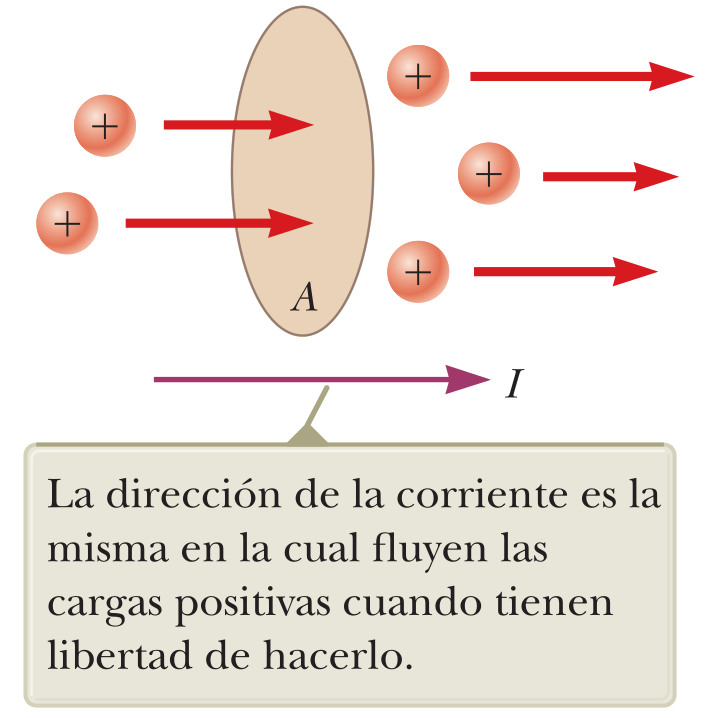
\includegraphics[width=\linewidth]{charges_flow.png}
    \caption{Cargas en movimiento a través de un área \(A\).}
    \label{fig:current}
\end{wrapfigure}

La corriente eléctrica es el flujo de carga eléctrica a través de un conductor. En un circuito eléctrico, la corriente se define como la cantidad de carga que pasa por unidad de area en un tiempo determinado. La unidad de medida de la corriente es el \hl{amperio} (\(A\)), que equivale a un culombio por segundo (\(C/s\)).

Cuando hablamos de \textbf{flujo de carga} nos referimos a la cantidad de carga que se mueve a través de una sección transversal del conductor en un tiempo determinado.

\subsubsection{Definición}

Para definir la corriente con mayor presición, suponga que las cargas tienen un movimiento perpendicular a una superficie \(A\), segun se observa en la figura \ref{fig:current}. La \textbf{corriente} se define como la tasa a la cual circula la carga a través de la superficie. Si \(\Delta Q\) es la carga que pasa a través de la superficie \(A\) en un intervalo de tiempo \(\Delta t\), la corriente promedio \(I_{prom}\) se define como:

\begin{equation}
    I_{prom} = \frac{\Delta Q}{\Delta t}
\end{equation}

Si la tasa a la que pasan las cargas varía en el tiempo, la corriente instantánea \(I\) se define como:
\[
    I = \lim_{\Delta t \to 0} \frac{\Delta Q}{\Delta t} = \frac{dQ}{dt}
\]

\begin{tcolorbox}[mydanger]
    \textbf{Cuidado:} la corriente es una magnitud \textit{escalar}. Por lo general describiremos la dirección de la corriente ya sea con palabras (por ejemplo, ``la corriente fluye por el circuito en el sentido horario'') o eligiendo una corriente como positiva si fluye en un sentido a lo largo de un conductor, y negativa si fluye en sentido contrario.
\end{tcolorbox}

\subsubsection{Movimiento de las cargas}
\label{sec:movimiento_de_cargas}

Para que exista un movimiento de cargas, es necesario que exista una fuerza que actúe sobre ellas. Esta fuerza es la fuerza eléctrica (ley de Coulomb: \ref{eq:ley_coulomb}) que actúa sobre las cargas libres (electrones) debido a la presencia de un campo eléctrico \(E\). Es decir, para que haya corriente eléctrica, debe existir un campo eléctrico que actúe sobre las cargas libres en el conductor. Este campo eléctrico puede ser generado por una diferencia de potencial entre dos puntos del conductor, como en el caso de una batería o una fuente de alimentación.

Cuando hay un campo eléctrico en un conductor, las cargas libres se aceleran y adquieren una velocidad. En palabras simples, podemos asociar la corriente eléctrica con el movimiento de cargas libres en un conductor.

En un conductor, los electrones libres se mueven en direcciones aleatorias debido a la temperatura del material. Sin embargo, cuando se aplica un campo eléctrico, estos electrones adquieren una velocidad de arrastre o \textbf{velocidad de deriva} \(v_d\) en la dirección del campo eléctrico. La velocidad de deriva es la velocidad promedio de las cargas (electrones en el caso de un conductor).

\begin{figure}[ht]
    \centering
    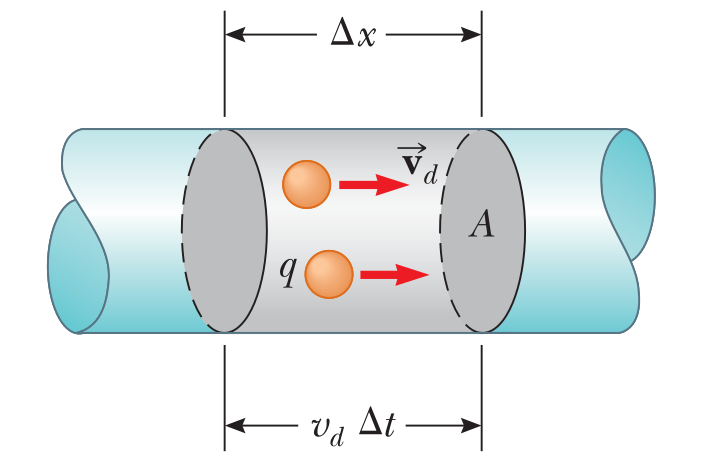
\includegraphics[width=0.5\textwidth]{v_d.png}
    \caption{Movimiento de cargas en un conductor.}
    \label{fig:movimiento_de_cargas_en_un_conductor}
\end{figure}

Recordando que \(\Delta Q\) es la cantidad de carga que pasa a través de la sección transversal \(A\), si tomamos un pedazo de conductor de longitud \(\Delta x\) como se muestra en la figura \ref{fig:movimiento_de_cargas_en_un_conductor}, podemos expresar el volúmen de este segmento de conductor como \(A \, \Delta x\). Si \(n\) es la densidad de carga (número de cargas por unidad de volumen), el número de cargas en el segmento es \(n A \Delta x\). Entonces la carga total de esta sección es:
\[
    \Delta Q = (n \, A \, \Delta x) \, q
\]
donde \(q\) es la carga de cada portador. Si tomamos un intervalo de tiempo \(\Delta t\) y consideramos que la velocidad promedio de las cargas es \(v_d\), el desplazamiento \(\Delta x\) se puede expresar como \(\Delta x = v_d \, \Delta t\). Entonces, podemos reemplazar \(\Delta x\) en la expresión de \(\Delta Q\):
\[
    \Delta Q = (n \, A \, v_d \, \Delta t) \, q
\]

Si dividimos ambos lados de la ecuación por \(\Delta t\), obtenemos la corriente promedio:
\[
    I_{prom} = \frac{\Delta Q}{\Delta t} = n \, A \, v_d \, q
\]

\begin{figure}[ht]
    \centering
    \begin{subfigure}[b]{0.4\textwidth}
        \centering
        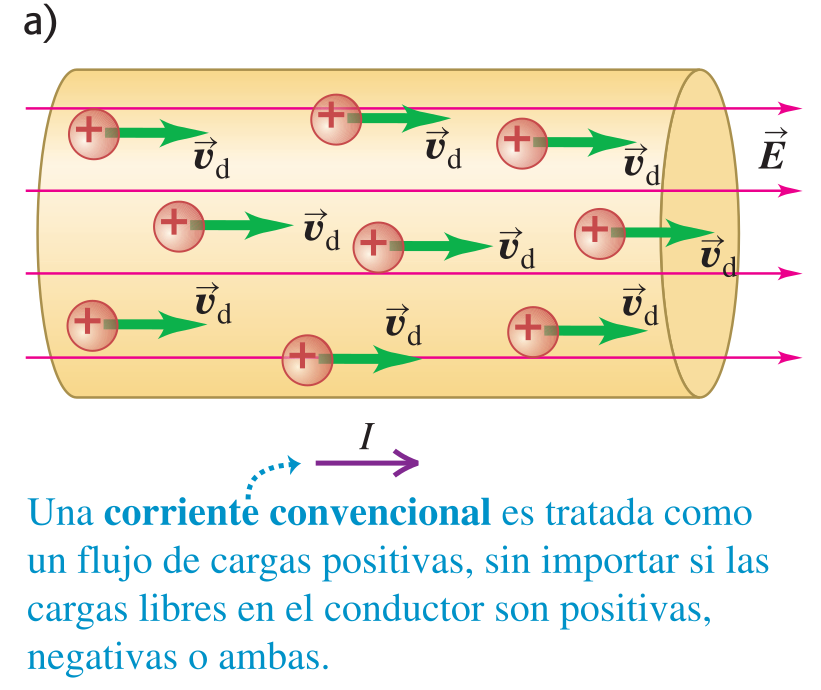
\includegraphics[width=\textwidth]{charges_movement_1.png}
        \caption{flujo de cargas positivas.}
        \label{fig:flujo_de_cargas_positivas}
    \end{subfigure}
    \hspace{10pt}
    \begin{subfigure}[b]{0.4\textwidth}
        \centering
        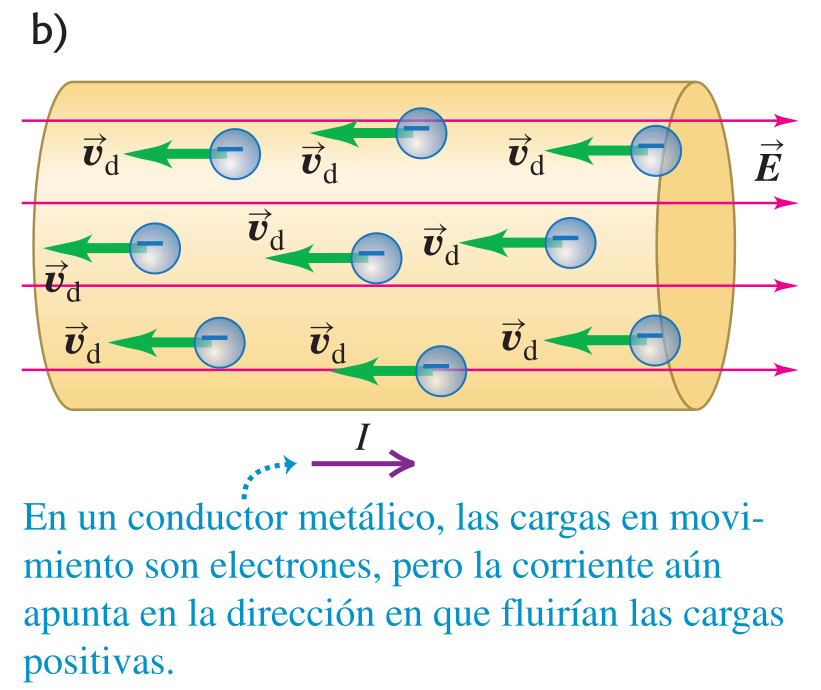
\includegraphics[width=\textwidth]{charges_movement_2.png}
        \caption{flujo de cargas negativas.}
        \label{fig:flujo_de_cargas_negativas}
    \end{subfigure}
    \caption{Flujo de cargas en un conductor.}
    \label{fig:flujo_de_cargas}
\end{figure}

La figura \ref{fig:flujo_de_cargas} presenta segmentos de material conductor. En la figura \ref{fig:flujo_de_cargas_positivas}, las cargas en movimiento son positivas, la fuerza eléctrica ocurre en la misma dirección que \(E\), y la velocidad de deriva \(v_d\) es de izquierda a derecha. En la figura \ref{fig:flujo_de_cargas_negativas} las cargas son negativas, la fuerza eléctrica es opuesta a \(E\), y la velocidad de deriva \(v_d\) es de derecha a izquierda. Definimos que la corriente, denotada por \(I\), va en la dirección en la que hay un flujo de carga positiva. Por ello, las corrientes se describen como si consistieran por completo en un flujo de cargas positivas, aun en los casos en que se sabe que la corriente real se debe a electrones. Así, en las figuras \ref{fig:flujo_de_cargas_positivas} y \ref{fig:flujo_de_cargas_negativas} la corriente es hacia la derecha. Esta convención sobre la dirección del flujo de la corriente se llama \textbf{corriente convencional}. Aunque la dirección de la corriente convencional no es necesariamente la misma en que se desplazan en realidad las partículas con carga, veremos que el signo de las cargas en movimiento tiene poca importancia en el análisis de los circuitos eléctricos.

\subsubsection{Densidad de corriente}

La densidad de corriente \(\vec{J}\) se define como la corriente por unidad de área transversal:
\[
\vec{J} = \frac{I}{A} \vec{u}
\]
donde \( I \) es la corriente, \( A \) es el área y \( \vec{u} \) es un vector unitario en la dirección del flujo de corriente.

Dado que la corriente \(I\) se puede expresar como \(n \, A\, v_d\, q\), la densidad de corriente se puede expresar como:
\[
\vec{J} = n q \vec{v}_d
\]

Es importante notar que la densidad de corriente es un vector, pero la corriente \(I\) no lo es. La diferencia está en que la densidad de corriente \(\vec{J}\) describe como fluyen las cargas en cierto punto, mientras que la corriente \(I\) describe la forma en la que fluyen las cargas a través de un objeto extendido. 

\subsection{Ley de Ohm}

\subsubsection{Resistividad}

La \textbf{resistividad} \(\rho\) de un material se define como la razón de las magnitudes del campo eléctrico y la densidad de corriete:
\begin{equation}
    \rho = \frac{E}{J} \quad [\Omega \cdot m]
\end{equation}

El recíproco de la resistividad es la conductividad \(\sigma\). Sus unidades son \((\Omega \cdot m)^{-1}\).
\begin{tcolorbox}[myconclusion]
\textbf{Importante:} Tanto la resistividad como la conductividad dependen del material y de factores como la temperatura.
\end{tcolorbox}

Tan pronto como se mantiene una diferencia de potencial a través del conductor se establece una densidad de corriente y un campo eléctrico. En algunos materiales, la densidad de corriente es proporcional al campo eléctrico:
\begin{equation}
\vec{J} = \sigma \vec{E} \qquad \leftrightarrow \qquad \vec{E} = \rho \vec{J}
\label{eq:forma_local_de_la_ley_de_ohm}
\end{equation}
donde la constante de proporcionalidad \(\sigma\) es la \textbf{conductividad} del conductor (\(1/\rho\)).

La relación de la ecuación \ref{eq:forma_local_de_la_ley_de_ohm} describe cómo un campo eléctrico induce una corriente en un medio conductor. Los materiales que obedecen dicha relación siguen la \textbf{ley de Ohm}.

\subsubsection{Formulando la ley de Ohm}

En estado estacionario, el campo eléctrico dentro de un conductor es constante en el tiempo. De la electrostática sabemos que:

\[
\Delta V = E \, d
\]

En un conductor rectilíneo y uniforme de longitud \( L \), la diferencia de potencial \( \Delta V \) entre sus extremos genera un campo uniforme, y despejando el campo en la ecuación anterior resulta:
\[
E = \frac{\Delta V}{L}
\]
Si el conductor tiene un área de sección transversal constante \( A \), y utilizando \( \vec{J} = \sigma \vec{E} \), la corriente total se deduce integrando la densidad de corriente sobre el área:
\[
I = \int_A \vec{J} \cdot d\vec{A} = J A = \sigma E A = \sigma \frac{\Delta V}{L} A
\]
De aquí se deduce la ley de Ohm macroscópica:
\begin{equation}
    \boxed{I = \frac{\sigma A}{L} \Delta V}
    \label{eq:ley_de_ohm}    
\end{equation}

\subsubsection{Resistencia}

La resistencia eléctrica se define como:
\[
R = \frac{\Delta V}{I} = \frac{L}{\sigma A}
\]

La inversa de la conductividad es la resistividad \( \rho \), por lo tanto:

\begin{equation}
    \boxed{R = \rho \frac{L}{A}}
    \label{eq:resistencia}
\end{equation}

\subsection{Aplicación de la ley de Ohm a circuitos}

\subsubsection{Circuitos en Serie}

Antes de comenzar es importante tener en cuenta que en un circuito en serie la corriente \( I \) es la misma en todos los elementos debido a que no hay bifurcaciones. Esto es debido a la conservación de la carga eléctrica y a la naturaleza de la conexión en serie.

Para entenderlo desde un enfoque físico, cuando varios elementos (resistencias, capacitores, etc.) están conectados en serie, sólo hay un camino posible para que circule la corriente eléctrica. Esto significa que las cargas eléctricas (generalmente electrones en un conductor metálico) no tienen bifurcaciones o alternativas en su trayecto: todas las cargas que pasan por un punto del circuito deben pasar por todos los demás puntos sucesivos en la misma rama.

Aplicando la ley de conservación de la carga (una consecuencia directa de la ley de continuidad en electromagnetismo), se deduce que no puede haber acumulación de carga en ningún punto del conductor en estado estacionario. Por tanto, el flujo de carga (es decir, la corriente) debe ser constante en todos los elementos conectados en serie. Si no fuera así, habría acumulación o desaparición de carga en algún nodo, lo cual no ocurre en un circuito cerrado en régimen permanente.

Es como el flujo de agua en una fuente; el agua brota de la parte superior de la fuente al mismo ritmo con el que llega a la parte inferior, sin importar las dimesiones de la fuetne. ¡El agua no ``se gasta'' a lo largo del trayecto!

En base a esta premisa, para cada resistencia, se cumple:

\[
V_i = I R_i
\]

La ley de Kirchhoff de tensiones establece que la suma de las caídas de potencial en una malla cerrada es igual a la fuente de tensión aplicada:

\[
V = V_1 + V_2 + \cdots + V_n = IR_1 + IR_2 + \cdots + IR_n
\]

Factorizando la corriente \( I \):

\[
V = I (R_1 + R_2 + \cdots + R_n)
\]

Definiendo la resistencia equivalente \( R_{\text{eq}} \) del sistema:

\[
\boxed{R_{\text{eq}} = R_1 + R_2 + \cdots + R_n}
\]

\paragraph{Ejemplo sencillo:}

Tres resistencias: \( R_1 = 2 \, \Omega \), \( R_2 = 3 \, \Omega \), \( R_3 = 5 \, \Omega \)

\[
R_{\text{eq}} = 2 + 3 + 5 = 10 \, \Omega
\]

Si se aplica una diferencia de potencial de \( V = 20 \, \text{V} \), entonces:

\[
I = \frac{V}{R_{\text{eq}}} = \frac{20}{10} = 2 \, \text{A}
\]

\subsubsection{Circuitos en Paralelo}

Al igual que en la sección anterior, vamos a partir con algunos supuestos físicos:
\begin{itemize}
    \item Las resistencias \( R_1, R_2, ..., R_n \) están conectadas en paralelo tienen sus terminales conectadas a los mismos dos nodos.
    \item La diferencia de potencial \( V \) es la misma en cada una.
    \item La corriente total se divide entre las ramas: \( I = I_1 + I_2 + \cdots + I_n \)
\end{itemize}

Entonces, aplicando la ley de Ohm y de la ley de Kirchhoff de corrientes

En cada resistencia, se cumple:

\[
I_i = \frac{V}{R_i}
\]

La corriente total será:

\[
I = \frac{V}{R_1} + \frac{V}{R_2} + \cdots + \frac{V}{R_n}
\]

Factorizando \( V \):

\[
I = V \left( \frac{1}{R_1} + \frac{1}{R_2} + \cdots + \frac{1}{R_n} \right)
\]

Definimos \( R_{\text{eq}} \) como la resistencia que satisface \( I = \frac{V}{R_{\text{eq}}} \). Entonces:

\[
\frac{V}{R_{\text{eq}}} = V \left( \sum_{i=1}^{n} \frac{1}{R_i} \right)
\Rightarrow \boxed{\frac{1}{R_{\text{eq}}} = \frac{1}{R_1} + \frac{1}{R_2} + \cdots + \frac{1}{R_n}}
\]

\paragraph{Ejemplo sencillo:}

Tres resistencias: \( R_1 = 4 \, \Omega \), \( R_2 = 6 \, \Omega \), \( R_3 = 12 \, \Omega \)

\[
\frac{1}{R_{\text{eq}}} = \frac{1}{4} + \frac{1}{6} + \frac{1}{12} = \frac{3 + 2 + 1}{12} = \frac{6}{12} = \frac{1}{2}
\Rightarrow R_{\text{eq}} = 2 \, \Omega
\]

\subsection{Energía y Potencia eléctrica}

Ahora abordaremos las expresiones teóricas de energía y potencia eléctrica en un circuito de corriente continua, partiendo de principios fundamentales. Estas magnitudes están directamente relacionadas con el trabajo que realiza el campo eléctrico sobre las cargas en movimiento. 

\subsubsection{Trabajo eléctrico}

Recordando lo que vimos en la unidad de electrostática, cuando una carga eléctrica \( q \) se desplaza entre dos puntos con diferencia de potencial \( \Delta V \), el trabajo realizado por el campo eléctrico es:

\[
W = q \Delta V
\]

Este trabajo es la energía transferida al sistema. Si en lugar de una sola carga \(q\) consideramos una corriente continua \( I \), que representa el flujo de carga por unidad de tiempo podríamos calcular el trabajo realizado por la corriente de cargas, entonces partir de la definición de corriente operamos para obtener una expresión para \(q\):

\begin{align*}
    I &= \frac{\Delta q}{\Delta t} \\
    I \Delta t &= \Delta q \\
    \Delta q &= I \Delta t
\end{align*}

Entonces, el trabajo realizado en ese intervalo de tiempo es:

\begin{equation}
    W = I \Delta V \, \Delta t
    \label{eq:trabajo_electrico}    
\end{equation}

\subsubsection{Potencia eléctrica}

La potencia es el trabajo realizado en un intervalo de tiempo, entonces la tasa de transferencia de energía (o trabajo realizado) por unidad de tiempo es:

\[
P = \frac{dW}{dt}
\]

Sustituyendo la expresión anterior para \( W \), obtenemos:

\begin{align}
    P &= \frac{d}{dt}(I \Delta V \, \Delta t) = I \Delta V \notag \\
    P &= IV
\end{align}

Esta expresión nos indica la potencia disipada (si \( V \) e \( I \) tienen el mismo signo) o suministrada (si tienen signos opuestos) en un componente del circuito.

Aplicando la ley de Ohm (\( V = IR \)) a la ecuación de potencia podemos encontrar la potencia disipada en una resistencia:

\[
P = VI = (IR)I = \boxed{P = I^2 R}
\]

Alternativamente, despejando la corriente de la ley de Ohm:

\[
I = \frac{V}{R} \Rightarrow P = V \left( \frac{V}{R} \right) = \boxed{P = \frac{V^2}{R}}
\]

Estas tres expresiones son equivalentes:

\begin{equation}
    \boxed{P = VI = I^2 R = \frac{V^2}{R}}
    \label{eq:potencia_electrica}
\end{equation}

y se usan dependiendo de qué variables sean conocidas en un circuito dado.


\subsubsection{Energía disipada en el tiempo}

Integrando la potencia en el tiempo se obtiene la energía total disipada o entregada:

\[
W = \int_{t_0}^{t_1} P \, dt = \int_{t_0}^{t_1} VI \, dt
\]

Si el circuito opera bajo condiciones constantes (circuito de corriente continua pura), entonces:

\[
W = V I \Delta t
\]

Si la resistencia es la única componente significativa, entonces:

\[
W = I^2 R \Delta t = \frac{V^2}{R} \Delta t
\]


\paragraph{Ejemplo sencillo}

Un resistor de \( R = 10 \, \Omega \) conectado a una batería de \( V = 12 \, \text{V} \), durante \( \Delta t = 30 \, \text{s} \).
\begin{itemize}
    \item Corriente: \( I = \frac{V}{R} = \frac{12}{10} = 1.2 \, \text{A} \)
    \item Potencia disipada: \( P = I^2 R = (1.2)^2 \cdot 10 = 14.4 \, \text{W} \)
    \item Energía disipada: \( W = P \Delta t = 14.4 \cdot 30 = 432 \, \text{J} \)
\end{itemize}

\subsection{Resumen}
\begin{tcolorbox}[title=Corriente Eléctrica]
  La corriente eléctrica es la tasa a la cual circula la carga a traves de una superficie.
  \[
    I_{prom} = \frac{\Delta Q}{\Delta t}
  \]
  que puede relacionarse con el movimiento de las cargas:
  \[
    I_{prom} = n q v_d A
  \]

  De esta ecuación se puede obtener la velocidad a la cual circulan los portadores de carga. La velocidad de deriva o arrastre es:
  \[
    v_d = \frac{I}{nqA}
  \]
  donde:
  \begin{itemize}
    \item \(I\) es la corriente que circula por el material
    \item \(q\) es la carga de los portadores (\(e=1.6\times10^{-19}\) en el caso de los electrones)
    \item \(A\) es el área transversal del material
    \item \(n\) es la densidad de portadores (el número de portadores) del el material por unidad de volumen.
  \end{itemize}

  Para obtener \(n\) para un material dado podemos usar la siguiente aproximación:
  \[
    n=\frac{\delta}{m_{molar}} N_A
  \]
  donde:
  \begin{itemize}
    \item \(\delta\) es la densidad del material
    \item \(m_{molar}\) es la masa molar del material
    \item \(N_A = 6.022 \times 10^{23} \, \mathrm{mol}^{-1}\) es el número de Avogadro.
  \end{itemize}
\end{tcolorbox}

\begin{tcolorbox}[title=Ley de Ohm]
  La ley de Ohm establece una relación de proporcionalidad entre la corriente, el potencial y la resistencia:
  \[
    V = IR
  \]
  \begin{itemize}
    \item La densidad de corriente es: \(\vec{J} = \sigma \vec{E}\)
    \item Ley de Ohm macroscópica: \(I = \frac{\sigma A}{L} \Delta V\)
    \item Definición de resistencia: \(R = \frac{\Delta V}{I} = \rho \frac{L}{A}\)
    \item Relación entre corriente y densidad de corriente: \(I = \int_A \vec{J} \cdot d\vec{A}\)
  \end{itemize}
  Estas ecuaciones permiten modelar y analizar cualquier sistema de corriente continua en conductores ohmicos.
\end{tcolorbox}


\begin{tcolorbox}[title=Circuitos]
  \subparagraph{Serie:}
  \begin{itemize}
    \item Corriente común: \( I = \text{constante} \)
    \item Tensión total: \( V = V_1 + V_2 + \cdots + V_n \)
    \item Resistencia equivalente: \(R_{\text{eq}} = \sum_{i=1}^{n} R_i\)
  \end{itemize}
  
  \subparagraph{Paralelo:}
  \begin{itemize}
    \item Tensión común: \( V = \text{constante} \)
    \item Corriente total: \( I = I_1 + I_2 + \cdots + I_n \)
    \item Resistencia equivalente: \(\frac{1}{R_{\text{eq}}} = \sum_{i=1}^{n} \frac{1}{R_i}\)
  \end{itemize}
\end{tcolorbox}


\begin{tcolorbox}[title=Trabajo y Potencia eléctrica]
  \subparagraph{Potencia general:}  
  
  \[
    P = V I
  \]
  
  \subparagraph{Potencia disipada en resistencias:}  
  \[
    P = I^2 R = \frac{V^2}{R}
  \]
  
  \subparagraph{Energía disipada o entregada en el tiempo \( \Delta t \):}
  \[
    W = P \Delta t = V I \Delta t = I^2 R \Delta t = \frac{V^2}{R} \Delta t
  \]
\end{tcolorbox}

\section{Electromagnetismo}

\subsection{Introducción}

El imán es un cuerpo o dispositivo con un magnetismo significativo, de forma que atrae a otros imanes o metales ferromagnéticos (por ejemplo, hierro, cobalto, níquel y aleaciones de estos). El magnetismo es el conjunto de fenómenos físicos mediados por campos magnéticos, que son una representación matemática del modo en que las fuerzas magnéticas interactúan y se distribuyen en el espacio.

\begin{figure}[ht]
  \centering
  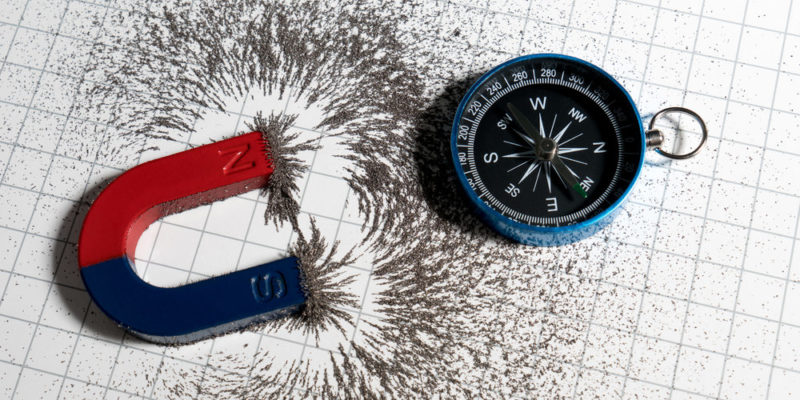
\includegraphics[width=0.5\textwidth]{iman-brujula.jpg}
  \caption{Limaduras de hierro y brújula afectados por un imán de herradura}
  \label{fig:iman}
\end{figure}

Como se puede apreciar en la figura \ref{fig:iman}, todos los imanes poseen dos polos, llamados \textit{polo norte} y \textit{polo sur}. Cualquiera de los polos de un imán atrae a un objeto ferromagnético no magnetizado, y, al igual que pasaba con las cargas eléctricas, los polos iguales se repelen y los polos opuestos se atraen. Es decir polo norte y polo sur se atraen, mientras que polo norte y polo norte (o sur y sur) se repelen.

La relación entre la electricidad y el magnetismo fue descubierta en 1819, cuando en el transcurso de una demostración en una conferencia, el científico danés Hans Christian Oersted descubrió que una corriente eléctrica en un alambre desviaba la aguja de una brújula cercana. Durante 1820, Faraday y Joseph Henry demostraron, de manera independiente relaciones adicionales entre la electricidad y el magnetismo. Mostraron que es posible crear una corriente eléctrica en un circuito ya sea moviendo un imán cerca de él o variando la corriente de algún circuito cercano. Estas observaciones demuestran que una variación en un campo magnético crea un campo eléctrico. Años después, el trabajo teórico de Maxwell demostró que lo contrario también es cierto: un campo eléctrico que varía crea un campo magnético.

\subsection{Magnetismo}

Tal vez el concepto de polos magnéticos parezca similar al de carga eléctrica, y los polos norte y sur parezcan análogos a las cargas positiva y negativa. No obstante, tal analogía puede ser errónea. Si bien las cargas positiva y negativa existen aisladas, no hay evidencia experimental de que exista un polo magnético aislado.

Los imanes siempre se encuentran como dipolos magnéticos (norte y sur), y no se ha comprobado la existencia los monopolos magnéticos.

\subsubsection{Campo Magnético}

Al igual que el campo eléctrico, el magnético es un \hl{\textit{campo vectorial}}, es decir, una cantidad vectorial asociada con cada punto del espacio. La existencia de un campo magnético en algún punto del espacio puede determinarse midiendo la magnitud de la \textbf{fuerza magnética} que ejerce el campo sobre una partícula de prueba ubicada en ese punto.

En esencia el magnetismo es un fenómeno físico asociado al movimiento de cargas eléctricas, que da lugar a fuerzas de atracción o repulsión entre materiales. Se manifiesta principalmente a través de los campos magnéticos, los cuales son representaciones vectoriales que describen la influencia que una corriente eléctrica o un material magnético ejerce en su entorno.

Desde un punto de vista fundamental, \hl{el origen del magnetismo reside en el movimiento de cargas eléctricas} a nivel microscópico, particularmente en el espín y el momento orbital de los electrones en los átomos. En materiales como el hierro, cobalto y níquel, estos momentos magnéticos atómicos se alinean de manera colectiva, generando imanes permanentes.

El \textbf{campo magnético} se representa mediante el vector \(\vec{B}\), cuya unidad en el Sistema Internacional es el tesla (T)\footnote{Un tesla equivale a: \(T \equiv \frac{Ns}{Cm} \equiv \frac{N}{Am}\)}. La interacción de una carga en \textbf{movimiento} \(q\) con un campo magnético está regida por la fuerza magnética, expresada como:
\begin{equation}
  \vec{F}_B = q\vec{v} \times \vec{B}
  \label{eq:fuerza_magnética}
\end{equation}
donde \(\vec{v}\) es el vector velocidad de la partícula. Esta fuerza es perpendicular tanto a la dirección de la velocidad como a la del campo magnético.

\begin{figure}[ht]
  \centering
  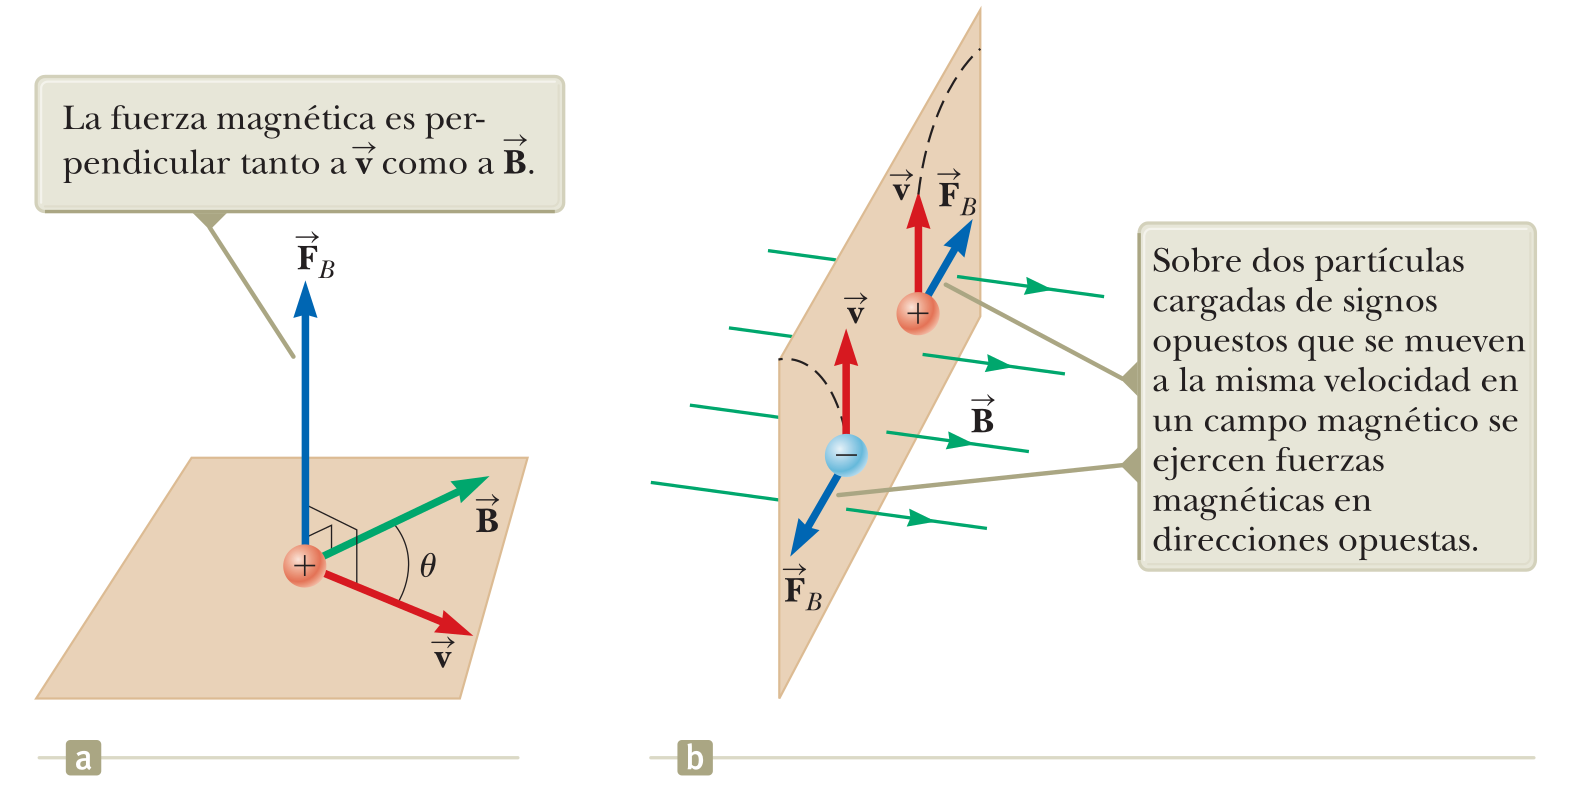
\includegraphics[width=0.8\textwidth]{magnetic_force.png}
  \caption{Partículas con carga atravesando un campo magnético \(\vec{B}\) con una velocidad \(\vec{v}\)}
\end{figure}

Si se conoce el ángulo \(\theta\) entre el vector velocidad \(\vec{v}\) y el campo magnético \(\vec{B}\) la fuerza se puede calcular como:
\[
  \vec{F}_B = \left\lvert q \right\rvert v B \sin(\theta) \hat{r}
\]
donde \(\hat{r}\) es un versor\footnote{versor: vector de módulo 1} normal al plano formado por los vectores \(\vec{v}\) y \(\vec{B}\). 

Comparando la fuerza magnética con la fuerza eléctrica se puede ver que la fuerza \(\vec{F}_B\) es perpendicular al campo magnético y a la velocidad de la partícula, mientras que \(\vec{F}_e\) se ejerce sobre la dirección del campo eléctrico. Además \(\vec{F}_e\) no requiere que la partícula con carga esté en movimiento.

\subsubsection{Lineas de campo magnético}

\begin{wrapfigure}{r}{0.3\textwidth}
  \centering
  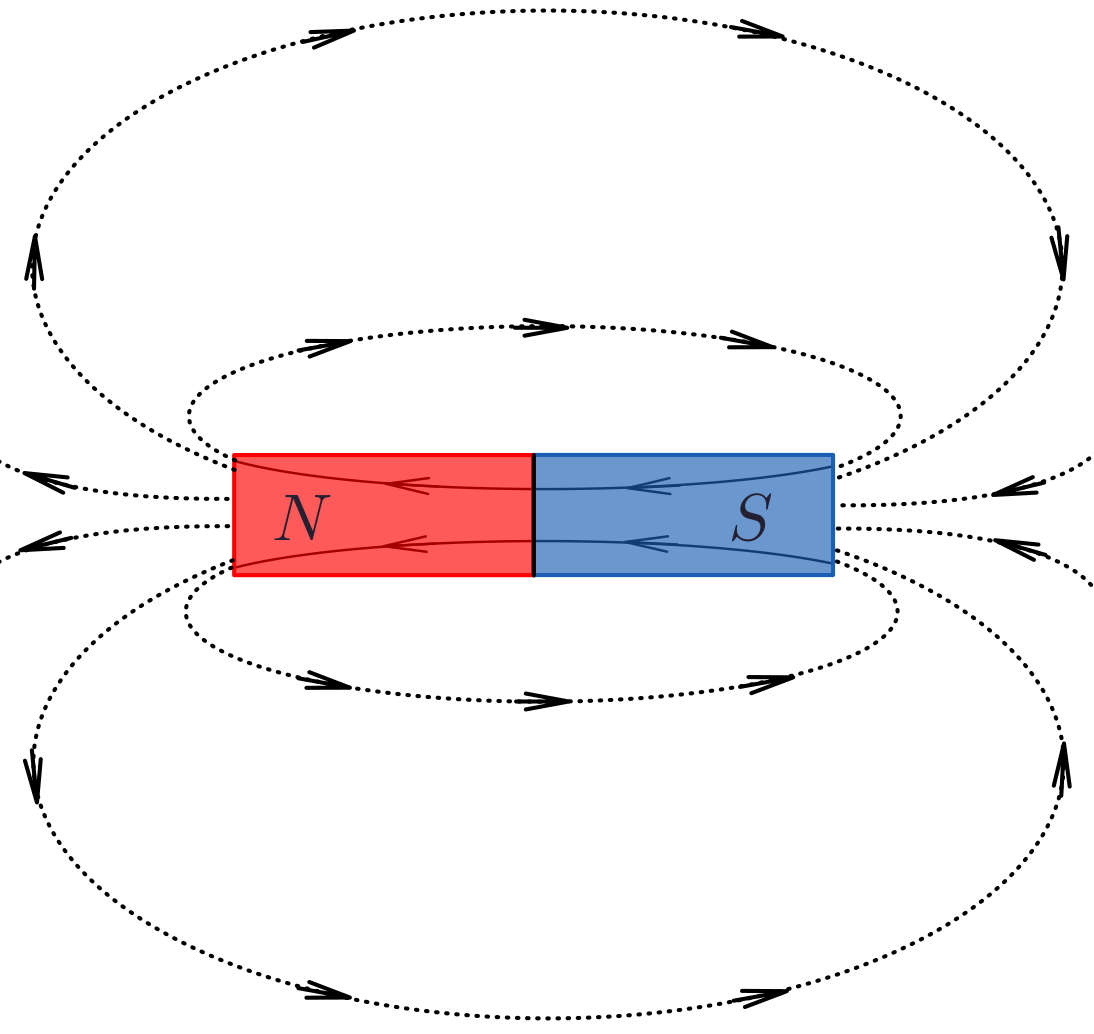
\includegraphics[width=\linewidth]{magnetic_field_lines.png}
  \caption{Líneas de campo magnético.}
  \label{fig:lineas_de_iman}
\end{wrapfigure}
La representación de los campos magnéticos mediante líneas de campo magnético es muy útil para visualizar la intensidad y la dirección del campo magnético. Como se muestra en la figura \ref{fig:lineas_de_iman}, cada una de estas líneas forma un bucle cerrado, aunque no se muestren todas las líneas cerradas por las limitaciones del espacio disponible puede observarse en las líneas de campo más cercanas al cuerpo del imán que salen del polo norte (\(N\)), hacen un bucle hacia el polo sur (\(S\)) y continúan a través de la barra magnética de vuelta al polo norte. Dentro del imán las líneas están muy juntas, pero nunca se cortan o tocan entre sí.

Las líneas de campo magnético tienen varias reglas estrictas:
\begin{enumerate}
  \item La dirección del campo magnético \(\vec{B}\) es tangente a la línea de campo en cualquier punto del espacio. Una pequeña brújula señalará la dirección de la línea del campo.
  \item La fuerza del campo es proporcional a la cercanía de las líneas. Es exactamente proporcional al número de líneas por unidad de superficie perpendicular a las líneas (llamada densidad de área). Es el mismo concepto que en las líneas de campo eléctrico. Mientras más juntas están mayor intensidad tiene.
  \item Las líneas de campo magnético no pueden cruzarse nunca, lo que significa que el campo es único en cualquier punto del espacio.
  \item Las líneas de campo magnético son continuas, formando bucles cerrados sin principio ni fin. Se dirigen del polo norte al polo sur.
\end{enumerate}

La última propiedad está relacionada con el hecho de que los polos norte y sur no pueden separarse. Es una diferencia clara respecto a las líneas de campo eléctrico, que generalmente comienzan en cargas positivas y terminan en cargas negativas o en el infinito. Si existieran cargas magnéticas aisladas (denominadas monopolos magnéticos), las líneas de campo magnético comenzarían y terminarían en ellas. Puedes ver más ejemplos sobre líneas de campo magnético en \href{https://openstax.org/books/f%C3%ADsica-universitaria-volumen-2/pages/11-2-campos-y-lineas-magneticas}{OpenStax} (\cite{openstax})

\begin{figure}[ht]
  \centering
  \begin{subfigure}[b]{0.35\textwidth}
      \centering
      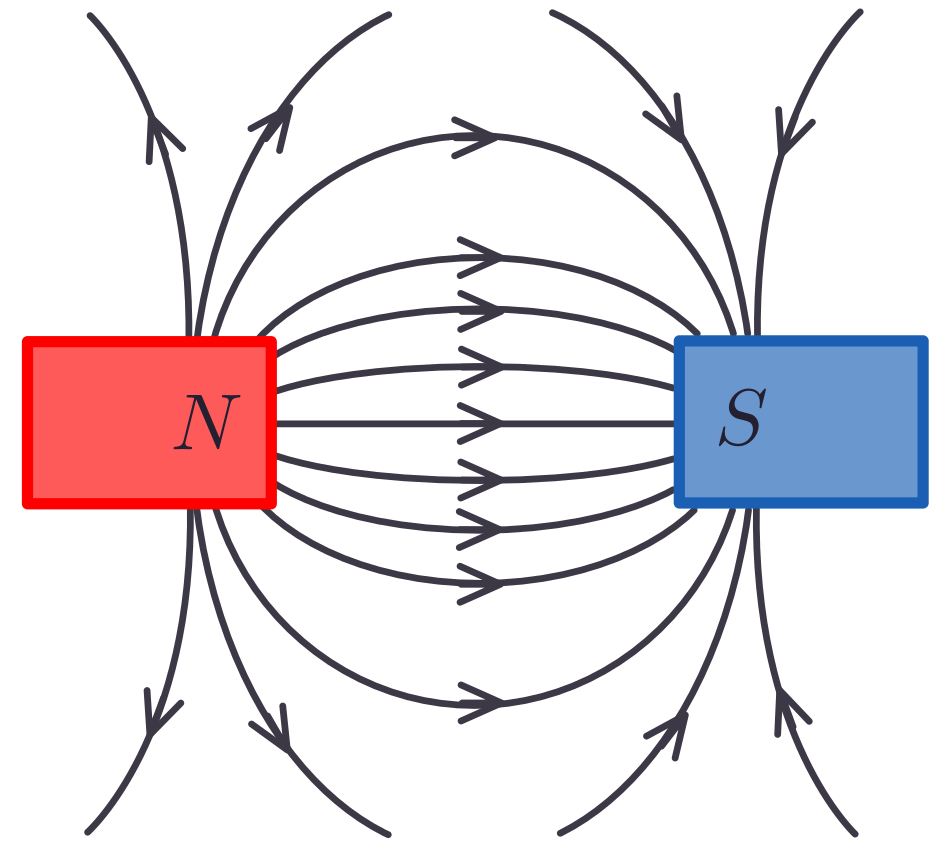
\includegraphics[width=\textwidth]{magnetic_lines_a.png}
      \caption{Líneas de campo magnético entre polos opuestos.}
      \label{fig:polos_opuestos}
  \end{subfigure}
  \hspace{10pt}
  \begin{subfigure}[b]{0.35\textwidth}
      \centering
      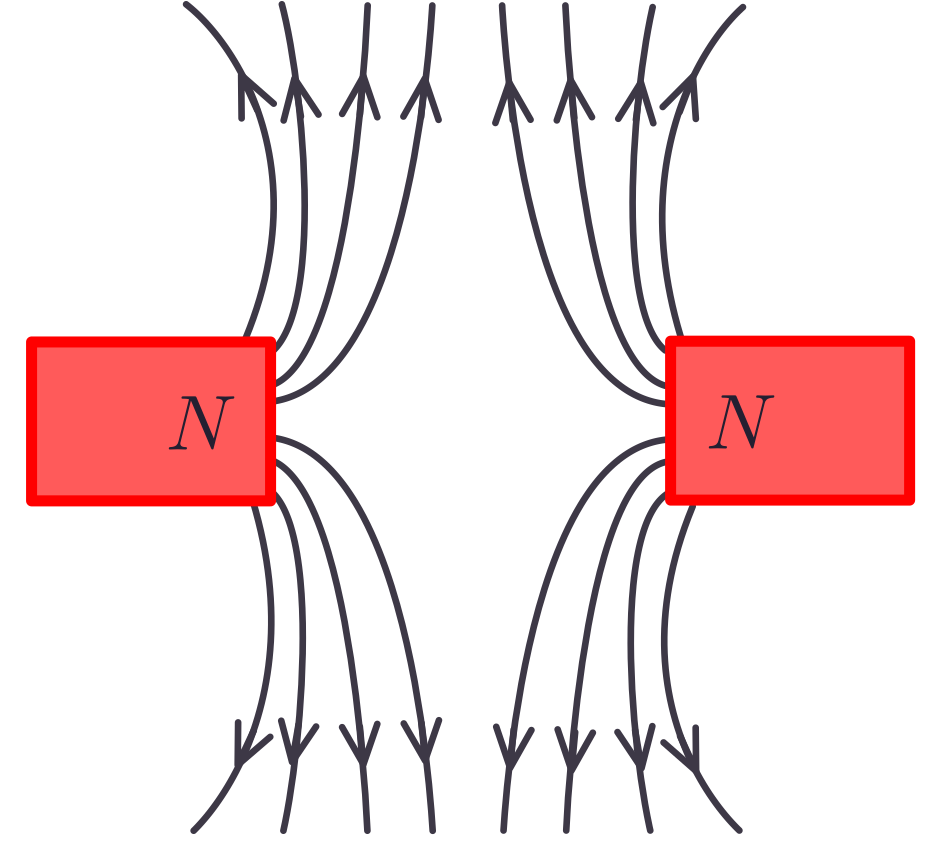
\includegraphics[width=\textwidth]{magnetic_lines_b.png}
      \caption{Líneas de campo magnético entre polos similares.}
      \label{fig:polos_iguales}
  \end{subfigure}
  \caption{Lineas de campo para distintas configuraciones de imanes.}
  \label{fig:lineas_de_campo_magnético_entre_imanes}
\end{figure}

Como se puede observar en la figura \ref{fig:lineas_de_campo_magnético_entre_imanes} las líneas de campo magnético se definen para tener la dirección en la que apunta una pequeña brújula cuando se coloca en un lugar del campo. La fuerza del campo es proporcional a la cercanía (o densidad) de las líneas. Si se pudiera sondear el interior del imán, se encontraría que las líneas de campo forman bucles continuos y cerrados. Para ajustarse a un espacio razonable, algunos de estos dibujos pueden no mostrar el cierre de los bucles; sin embargo, si se dispusiera de espacio suficiente, los bucles estarían cerrados. 

Nótese que en la figura \ref{fig:polos_opuestos} el campo que se forma en el centro de los imanes es casi uniforme. Este concepto es útil ya que este tipo de campo se encuentra en los imanes de herradura (como el que está en la figura \ref{fig:iman}). Por otro lado en la figura \ref{fig:polos_iguales} el campo entre imanes es casi cero (muy poca intensidad) ya que las líneas de campo magnético están muy separadas entre sí.

\subsubsection{Flujo Magnético}
\label{sec:flujo_magnético}

Definimos el \textbf{flujo magnético} \(\Phi_B\) a través de una superficie igual que definimos el flujo eléctrico en relación con la ley de Gauss en la sección \ref{sec:flujo_electrico}. 

El flujo magnético es una magnitud escalar que cuantifica la cantidad de campo magnético que atraviesa una superficie dada. Matemáticamente, se define como la integral del producto escalar entre el campo magnético \(\vec{B}\) y el vector diferencial de área \(d\vec{A}\) de la superficie:

\[
\Phi_B = \int_S \vec{B} \cdot d\vec{A}
\]
donde:
\begin{itemize}
  \item \(\Phi_B\) es el flujo magnético,
  \item \(S\) es la superficie sobre la que se calcula el flujo,
  \item \(\vec{B}\) es el vector del campo magnético,
  \item \(d\vec{A}\) es un elemento diferencial de área, cuyo módulo es el área diferencial y cuya dirección es perpendicular a la superficie, siguiendo la convención del sentido positivo (normal saliente en una superficie cerrada).
\end{itemize}

Al igual que el flujo eléctrico, el flujo magnético mide cuántas ``líneas de campo magnético'' atraviesan una superficie. Si el campo es perpendicular a la superficie, el flujo es máximo; si es paralelo, el flujo es nulo.

En el caso especial donde el campo magnético es uniforme y la superficie es plana, la expresión se simplifica a:
\[
\Phi_B = B A \cos\theta
\]
donde:
\begin{itemize}
  \item \(B\) es la magnitud del campo magnético,
  \item \(A\) es el área de la superficie,
  \item \(\theta\) es el ángulo entre el vector \(\vec{B}\) y el vector normal a la superficie.
\end{itemize}

La unidad de flujo magnético en el Sistema Internacional es el weber (Wb), donde: \(1 \, \text{Wb} = 1 \, \text{T} \cdot \text{m}^2\)

Si recuerda el \textit{flujo eléctrico} y la ley de Gauss de la sección \ref{sec:ley_de_gauss} podríamos intuir que para el magnetismo pasa algo similar. Sin embargo como no existen los monopolos magnéticos y las líneas de campo magnético son cerradas \hl{el flujo magnético sobre una superficie cerrada es siempre cero.}
\[
\oint \vec{B}\cdot d\vec{A} = 0
\]
Digamos, en palabras simples: si encerramos un imán en una superficie Gaussiana, todas las líneas de campo magnético que salen, vuelven a entrar. Esto resulta en un flujo nulo.

\subsubsection{Trabajo del campo magnético}

En la sección \ref{sec:potencial} vimos como una carga que se mueve en un campo eléctrico realiza un trabajo. En esta sección las partículas deben estar si o si en movimiento para verse afectadas por el campo magnético. Entonces ¿Será que están realizando trabajo? La respuesta rápida es que no. Veamos el por qué: recordando que el trabajo es el \textbf{producto escalar} entre la fuerza por la distancia (o desplazamiento), si la fuerza es perpendicular al desplazamiento entonces dará siempre cero.
En base a esto, vemos que \(\vec{F}_B\) no realiza trabajo ni cambia la energía del sistema carga-campo por ser perpendicular al plano de \(\vec{B}\) y \(\vec{v}\). 

\begin{tcolorbox}[myconclusion]
  Con base en este último enunciado y también con el teorema trabajo-energía cinética, se concluye que la energía cinética de una partícula cargada que se mueve a través de un campo magnético \textbf{no} puede ser modificada sólo por el campo magnético. El campo magnético puede modificar la dirección del vector velocidad, pero no puede cambiar la rapidez ni la energía cinética de la partícula.
\end{tcolorbox}

\begin{wrapfigure}{l}{0.3\textwidth}
  \centering
  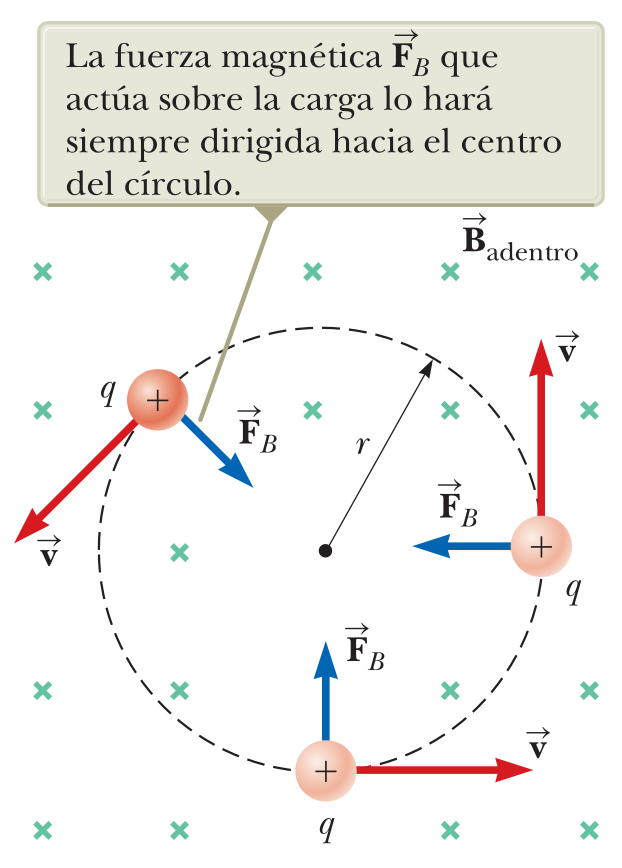
\includegraphics[width=\linewidth]{centipet_force.png}
  \caption{Fuerza magnética para una partícula con velocidad \(v\) y un campo magnético entrante.}
  \label{fig:centripet_force}
\end{wrapfigure}
\subparagraph{Pregunta:}

\noindent ¿Qué tipo de fuerza es siempre perpendicular a la trayectoria de una partícula y no modifica la magnitud de la velocidad?

\vspace{3pt}

\noindent La \textbf{fuerza centrípeta}. Entonces, la fuerza magnética, como se ve en la figura \ref{fig:centripet_force} es una fuerza centrípeta para una partícula cargada y en movimiento. Por lo tanto podemos ocupar todas las ecuaciones del movimiento circular.

Si no recuerdas bien los temas de dinámica y las ecuaciones del movimiento circular uniforme y no uniforme puedes volver a verlo en la sección \ref{sec:mcu}

Con este principio, se observa que para la situación ilustrada en la figura \ref{fig:centripet_force} la magnitud de \(\vec{F}_B\) y \(\vec{v}\) son constantes. Como \(\vec{F}_B \equiv \vec{F}_c\) entonces podemos igualar \(\vec{F}_B\) a la expresión de aceleración centrípeta:
\[
  F_B = qvB = m \frac{v^2}{r}
\]
\clearpage

\subsection{Fuerza de Lorentz}

Una carga móvil con una velocidad \(\vec{v}\), en presencia tanto de un campo eléctrico \(\vec{E}\) como de un campo magnético \(\vec{B}\) es descrito por dos modelos de partícula en un campo. Experimenta a la vez una fuerza eléctrica \(\vec{F}_E=q\vec{E}\) y una fuerza magnética \(\vec{F}_B=q\vec{v} \times \vec{B}\). La fuerza total es la fuerza de Lorentz:

\begin{equation}
  \vec{F} = q\left(\vec{E} + \vec{v} \times \vec{B}\right)
  \label{eq:f_lorentz}
\end{equation}

\subsubsection{Fuerza magnética en un conductor}
\label{sec:fuerza_magnetica_en_un_conductor}

\begin{wrapfigure}{r}{0.3\textwidth}
  \centering
  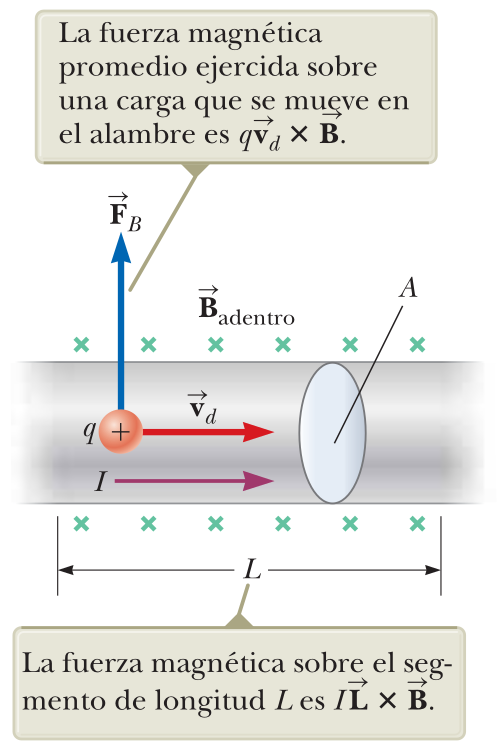
\includegraphics[width=0.3\textwidth]{lorentz.png}
  \caption{Un segmento de un alambre conduciendo corriente en un campo magnético \(\vec{B}\)}
  \label{fig:lorentz}
\end{wrapfigure}
Ahora hagamos un análisis de las fuerzas que interactúan para un cable conductor como el que se muestra en la figura \ref{fig:lorentz}. Vemos que en la figura el campo magnético es entrante. Si no circula corriente eléctrica, entonces no hay movimiento de cargas, por ende las cargas tendrán una \(v_d=0\) y la fuerza magnética será cero. Si hacemos circular cargas sobre el conductor aplicando una diferencia de potencial entre las puntas del conductor, entonces \(v_d \neq 0\) y por lo tanto existirá una fuerza magnética. 
Conviene cuantificar esta explicación considerando la longitud \(L\) del segmento y el área de sección transversal \(A\). Al tener en cuenta las dimensiones del cable, podemos expresar la \textbf{fuerza total} que sentirá el cable. Sabiendo que la corriente que circula por el cable es \(I = nq v_d A\) y el volumen del cable es \(AL\) entonces: 
\[
  \vec{F}_B = (q\vec{v}_d \times \vec{B})nAL
\]
Reemplazando \(I=qn \vec{v}_d A\) en la expresión:
\[
  \vec{F}_B = I\vec{L} \times \vec{B}
\]
donde \(\vec{L}\) es un vector que apunta en la dirección de la corriente \(I\) y tiene una magnitud igual a la longitud \(L\). Si se expresa el producto vectorial como el módulo de los vectores por el seno del ángulo entre ellos:
\begin{equation}
  \boxed{F_B = IL \cdot B \, \sin(\theta)}
  \label{eq:fuerza_magnetica_en_un_conductor}
\end{equation}

\subsection{Momento de torsión sobre una espira}

Es importante que antes de abordar esta sección se haya entendido bien la sección anterior (\ref{sec:fuerza_magnetica_en_un_conductor}) y que recuerde qué es torque. Si desea ver un recordatorio sobre torque puede utilizar el resumen dado en la sección \ref{sec:torque_y_momento_de_inercia}.

\subsubsection{Definición de espira}

Tal vez parezca trivial definir el concepto de espira, sin embargo vamos a aclarar los elementos que vamos a usar para demostrar cómo generamos el par de torsión. Entonces, una espira es un lazo de alambre por el que puede fluir corriente eléctrica. Vamos a tomar una espira rectangular, y vamos a suponer que fluye una corriente como se muestra en la figura \ref{fig:espira_vista_superior}. En este caso estamos ignorando de dónde proviene la corriente eléctrica, y suponiendo que la espira es totalmente cerrada.
\begin{wrapfigure}{l}{0.3\textwidth}
  \centering
  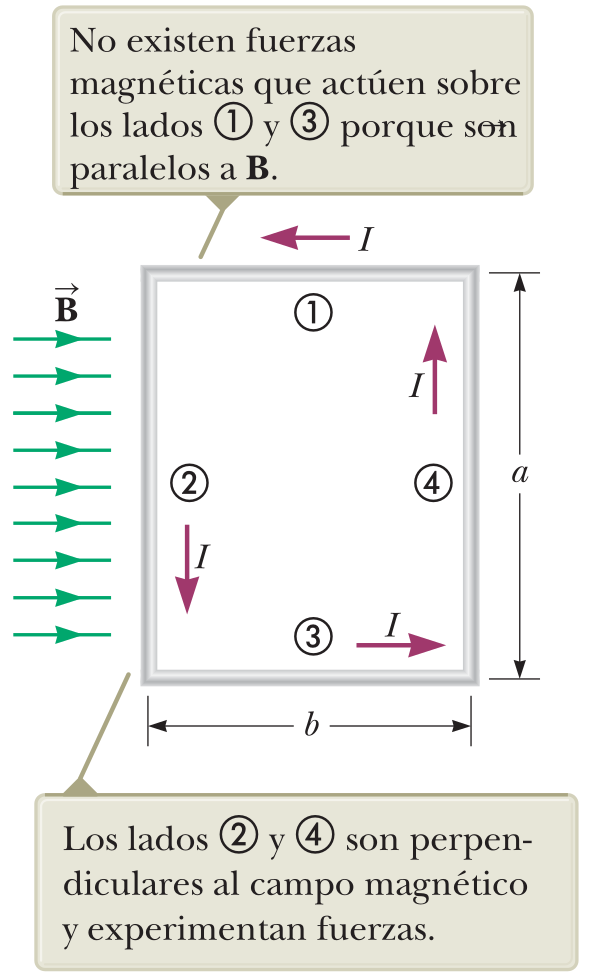
\includegraphics[width=\linewidth]{espira_sup.png}
  \caption{Vista superior de una espira rectangular}
  \label{fig:espira_vista_superior}
\end{wrapfigure}

Cuando la corriente pasa a través de la espira, las cargas fluyen a través del conductor (de la misma forma que vimos en la sección anterior). Si se coloca en un campo magnético uniforme \(\vec{B}\) de modo que sea perpendicular a dos de los segmentos (el segmento \textcircled{2} y \textcircled{4} en caso de la figura \ref{fig:espira_vista_superior}), cada uno experimenta una fuerza magnética dada por la ecuación \eqref{eq:fuerza_magnetica_en_un_conductor} mientras que en los segmentos \textcircled{1} y \textcircled{3} la fuerza magnética será nula ya que el vector \(\vec{v}_d\) y \(\vec{B}\) son paralelos. 

Las fuerzas que actúan sobre los segmentos \textcircled{2} y \textcircled{4} no se cancelan completamente en su efecto mecánico: aunque su suma vectorial puede ser nula (es decir, no producen una traslación neta de la espira), sí generan un momento de torsión o torque que tiende a rotarla.

Entonces, teniendo en cuenta que la longitud de los segmentos \textcircled{2} y \textcircled{4} es \(L=a\), el módulo de la fuerza que siente cada segmento será:
\begin{equation}
  F_{2} = F_{4} = IaB
  \label{eq:fuerza_torque_en_una_espira}
\end{equation}

\begin{tcolorbox}[myconclusion]
  Recuerda: Esta fuerza es perpendicular tanto al elemento de corriente como al campo magnético.
\end{tcolorbox}

\subsubsection{Definición de momento de torsión}

\begin{wrapfigure}{l}{0.3\textwidth}
  \centering
  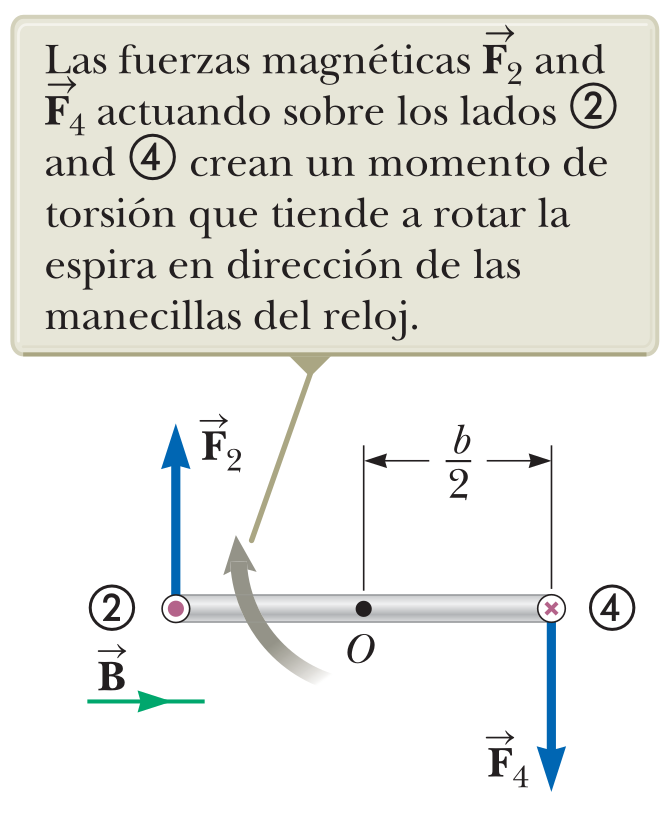
\includegraphics[width=\linewidth]{espira_lat.png}
  \caption{Vista lateral de la espira rectangular}
  \label{fig:espira_vista_lateral}
\end{wrapfigure}
Si analizamos la misma espira de la figura \ref{fig:espira_vista_superior} pero vista desde el lateral para poder visualizar las fuerzas actuantes podemos ver por qué se produce un torque.

Si se aplica la regla de la mano derecha en la figura \ref{fig:espira_vista_superior} podemos ver que en el segmento \textcircled{2} la fuerza es saliente y en el segmento \textcircled{4} la fuerza es entrante. Si vemos la figura \ref{fig:espira_vista_lateral} donde se muestra la misma espira en vista lateral, vemos que sobre el segmento \textcircled{2} la fuerza actúa hacia arriba y sobre el segmento \textcircled{4} actúa hacia abajo. Estas fuerzas no pueden provocar una traslación ya que se cancelan entre sí, pero si pueden provocar una rotación respecto de un eje \(O\).

Sabemos que el módulo del momento de torsión o torque (\(\tau\)) respecto de un eje de giro \(O\) es:
\begin{align*}
  \tau &= F\, r \sin(\theta) \\
  \text{Y}&\,\text{para dos fuerzas actuantes:}\\
  \tau &= \tau_1 + \tau_2 \\
  \tau &= F_1 r_1 \sin(\theta_1) + F_2 r_2 \sin(\theta_2)  
\end{align*}

En nuestra espira, el ángulo \(\theta=\pi/2\) será el mismo para las dos fuerzas \(F_{2}\) y \(F_{4}\), ya que depende del ángulo de la espira con \(\vec{B}\).

En base a esto, entonces observando la figura \ref{fig:espira_vista_lateral} podemos aplicar la expresión de torque a las fuerzas que actúan sobre la espira, resultando:
\begin{align}
  \tau &= F \, r \, \sin(\theta); \quad \text{donde para cada lado: } F=F_B ~~\text{y}~~ r=b/2 \nonumber \\ 
       &= F_{2} \, \frac{b}{2}\, \sin(\theta) + F_{4} \, \frac{b}{2}\, \sin(\theta) \nonumber \\
       &= \left(IaB + IaB\right)\, \frac{b}{2} \, \sin(\theta); \quad \text{donde:}~~ L=a \nonumber \\ 
       &= 2IaB \, \frac{b}{2} \, \sin(\theta) \nonumber \\
       &= IB \, ab \, \sin(\theta); \quad \text{como} ~~ A=ab \nonumber \\
  \tau &= IB \, A \, \sin(\theta)
  \label{eq:torque_para_una_espira}
\end{align}

En este caso como \(\theta = \pi/2\) se obtiene el torque máximo \(\tau_{max} = IAB\), sin embargo la expresión \eqref{eq:torque_para_una_espira} funciona para cualquier ángulo \(\theta\) que forme la espira con respecto a \(\vec{B}\). 

Sabemos que como el torque es definido como producto vectorial entonces \(\tau\) es un vector perpendicular al plano formado por otros dos vectores. En el caso de la espira, como vimos durante el desarrollo \eqref{eq:torque_para_una_espira} sabemos que el campo magnético \(\vec{B}\) es un vector. El otro vector será el área \(\vec{A}\) y, al igual que lo definimos en el flujo eléctrico y magnético, es un vector perpendicular a la superficie. Para comprender mejor el vector área de la espira, puede observarlo en la figura \ref{fig:espira_rotada}

\begin{figure}[ht]
  \centering
  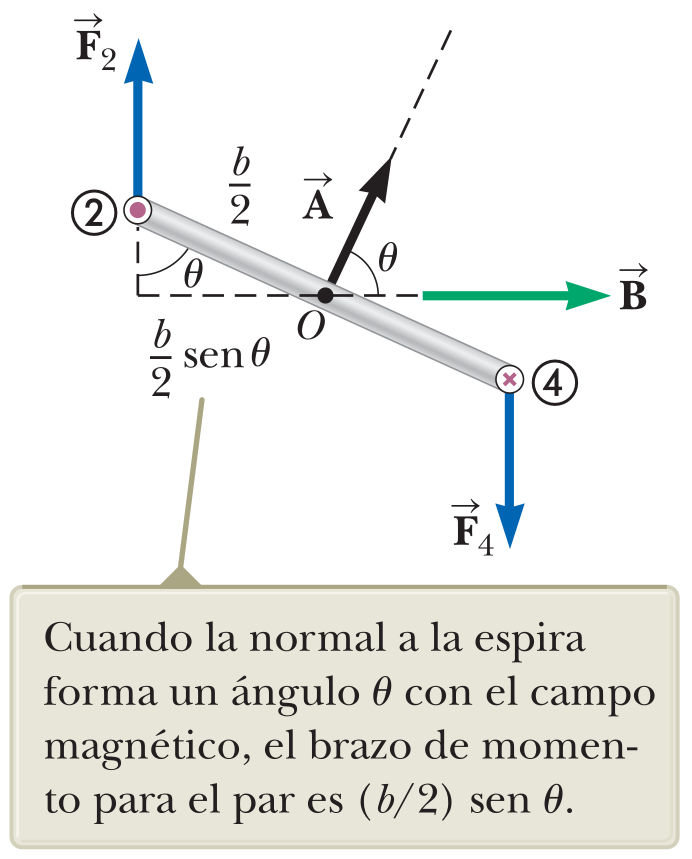
\includegraphics[width=0.4\textwidth]{espira_lat_theta.png}
  \caption{Vista lateral de la espira rectangular rotada un ángulo \(\theta\)}
  \label{fig:espira_rotada}
\end{figure}

En base a esto entonces decimos que \(\vec{tau}\) para una espira es:
\begin{equation}
  \boxed{\vec{\tau} = I\vec{A}\times \vec{B}}
  \label{eq:vec_torque_de_espira}
\end{equation}

Aunque la ecuación \ref{eq:vec_torque_de_espira} se dedujo para una espira rectangular, es válida para una espira plana de cualquier forma.

\subsubsection{Momento dipolar magnético}

El \textbf{momento dipolar magnético} de una \textit{espira} es una \hl{cantidad vectorial} que caracteriza la intensidad y la orientación del campo magnético generado por una corriente eléctrica que circula por una espira cerrada\footnote{En el Sistema Internacional, se mide en \(\text{A·m}^2\) (amperio-metro cuadrado).}.
\[
  \vec{\mu} = I \vec{A}
\]

\begin{wrapfigure}{r}{0.27\textwidth}
  \centering
  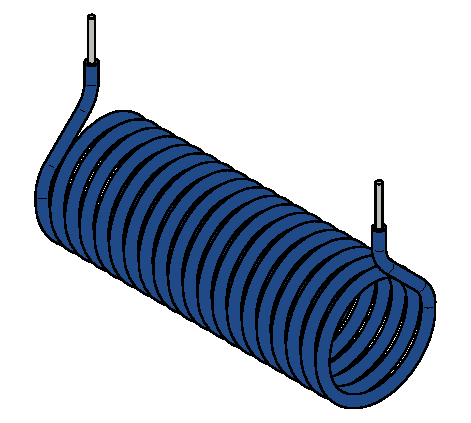
\includegraphics[width=\linewidth]{Solenoid.pdf}
  \caption{Imágen de un solenoide}
  \label{fig:solenoide}
\end{wrapfigure}
Su magnitud está dada por el producto de la corriente eléctrica (\(I\)) que fluye por la espira y el área (\(A\)) encerrada por esta:  
\[
  \mu = I A
\]  
Si se tiene un solenoide de \(N\) vueltas (o espiras), el momento se amplifica:  
\[
  \mu = N I A
\]

\begin{tcolorbox}
  \textbf{Nota}: el término \textit{espira} se suele usar para referirse a un solo lazo de alambre, mientras que un solenoide consiste en múltiples espiras enrolladas en forma de cilindro como se muestra en la figura \ref{fig:solenoide}.
\end{tcolorbox}

\(\vec{A}\) es el vector área de una sola espira o vuelta, su magnitud es el área \(A\) de la espira (por ejemplo en la figura \ref{fig:dipolar_magnet_moment} el área de la espira será \(A=\pi r^2\)), y su dirección es normal al plano de la espira, siguiendo la regla de la mano derecha respecto al sentido de la corriente. Si los dedos de la mano derecha se curvan en el sentido de la corriente, el pulgar apunta en la dirección del vector momento dipolar magnético (\(\vec{\mu}\)), perpendicular al plano de la espira.
\begin{figure}[ht]
  \centering
  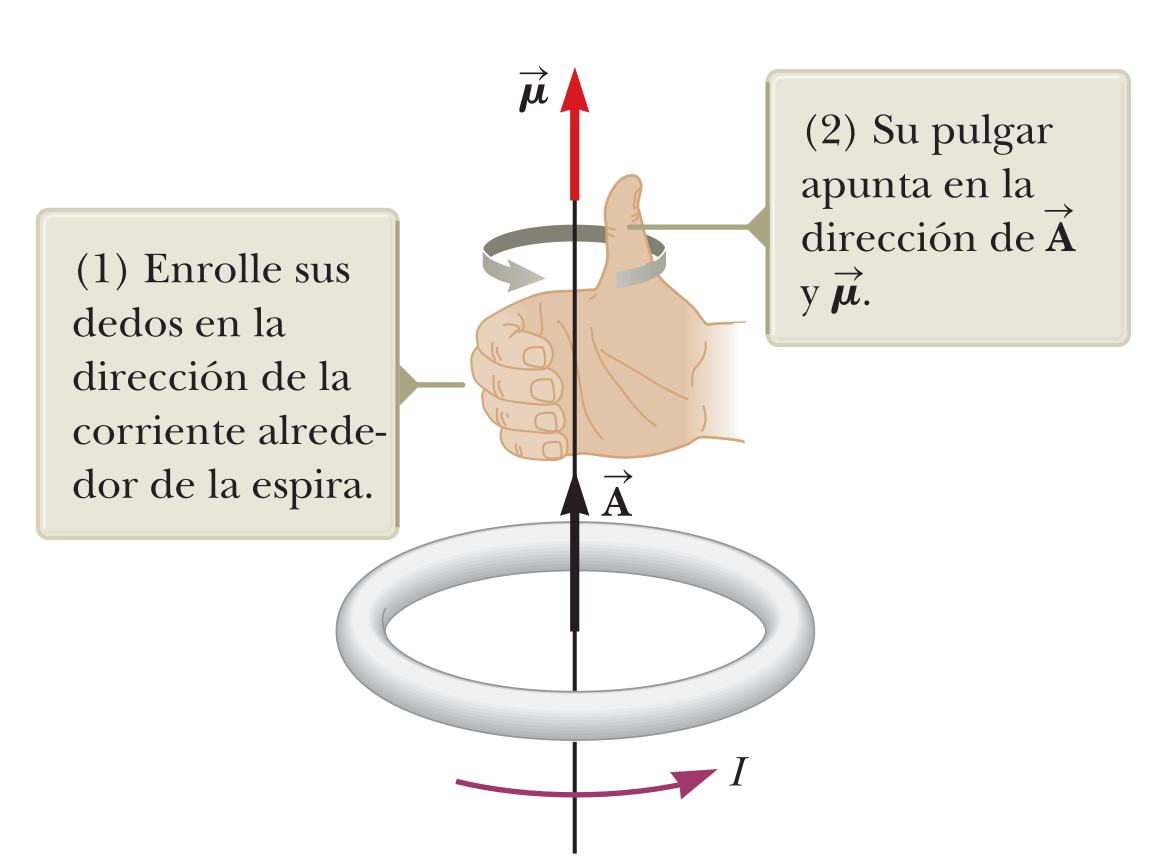
\includegraphics[width=0.5\textwidth]{dipolar_magnet_moment.png}
  \caption{Regla de la mano derecha para determinar la dirección del vector \(\vec{A}\) y el momento dipolar magnético \(\vec{\mu}\).}
  \label{fig:dipolar_magnet_moment}
\end{figure}

En base al momento dipolar magnético, se puede escribir una expresión de torque (\(\vec{\tau}\)) que experimenta un solenoide de \(N\) vueltas en presencia de un campo magnético externo (\(\vec{B}\)): 
\[
  \vec{\tau} = \vec{\mu} \times \vec{B}
\]

Si el momento magnético \(\vec{\mu}\) es paralelo al campo \(\vec{B}\), no hay momento de torsión (\(\tau = 0\)). Si \(\vec{\mu}\) es perpendicular a \(\vec{B}\), el momento de torsión es máximo. El torque tiende a alinear \(\vec{\mu}\) con \(\vec{B}\).

\begin{figure}[ht]
  \centering
  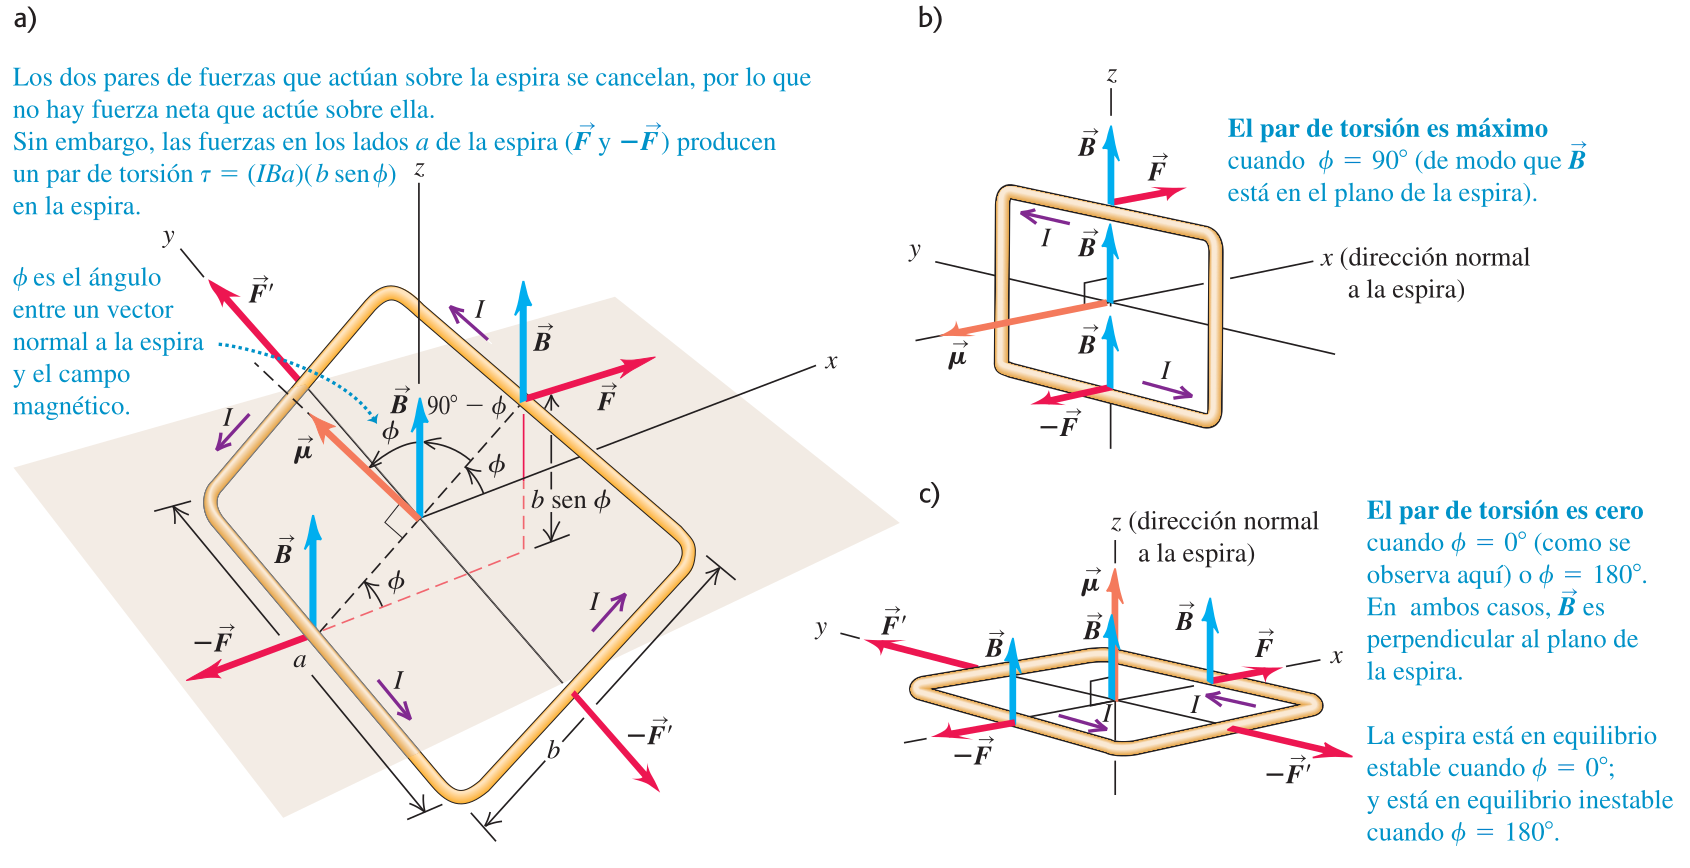
\includegraphics[width=1\textwidth]{par.png}
  \caption{Cálculo del par de torsión sobre una espira que conduce corriente en un campo magnético uniforme.}
\end{figure}

\begin{tcolorbox}[myconclusion]
  El momento magnético mide cuán magnético es un cuerpo, en el mismo sentido que el momento angular mide cuán rotacional es, y el momento lineal cuán translacional.
\end{tcolorbox}

Cuando un sistema con momento magnético \(\vec{\mu}\) se coloca en un campo magnético externo \(\vec{B}\), experimenta:
\begin{itemize}
  \item \textbf{Un torque}: \(\vec{\tau}=\vec{\mu}\times\vec{B}\) que lo alinea con el campo,
  \item \textbf{Una energía potencial}: \(U=-\vec{\mu}\cdot\vec{B}\), mínima cuando \(\vec{\mu}\) y \(\vec{B}\) están alineados.
\end{itemize}
Esto explica fenómenos como la orientación de las agujas magnéticas, el paramagnetismo, y técnicas como la resonancia magnética nuclear (RMN).

\begin{tcolorbox}[mydanger]
  \textbf{CUIDADO}: Una partícula cargada que se mueve \textbf{en línea recta} a \textit{velocidad constante} \textbf{no tiene momento magnético} (aunque sí genera un campo magnético). El momento magnético aparece solo cuando hay \textbf{movimiento cerrado o rotacional}, como una espira de corriente o una órbita de una partícula. Cuanto mayor es el momento magnético, más fuertemente responde el sistema ante un campo magnético externo, tanto en torque como en energía potencial.
\end{tcolorbox}

Puede ampliar los contenidos de torque magnético en \href{https://openstax.org/books/f%C3%ADsica-universitaria-volumen-2/pages/11-5-fuerza-y-torque-en-un-bucle-de-corriente}{OpenStax} \cite{openstax}.

\begin{tcolorbox}[interesting_data, title=Dato curioso]
  Una aplicación médica importante del par de torsión sobre un dipolo magnético son las imágenes de resonancia magnética (IRM). Se coloca a un paciente en un campo magnético de aproximadamente \(1.5 \si{\tesla}\), lo cual es \(10^4\) veces más intenso que el campo de la Tierra. El núcleo de cada átomo de hidrógeno en el tejido que se desea observar tiene un momento dipolar magnético, que experimenta un par de torsión que lo alinea con el campo aplicado. Después se ilumina el tejido con ondas de radio de la frecuencia correcta para apenas sacar a estos momentos magnéticos de su alineación. El grado en que estas ondas de radio son absorbidas por el tejido es proporcional a la cantidad de hidrógeno presente. De ahí que un tejido suave rico en hidrógeno se vea muy distinto de un hueso con poco hidrógeno, lo cual hace que la IRM sea ideal para analizar detalles de tejidos suaves que no se verían en las imágenes de rayos x  
\end{tcolorbox}

\subsection{Fuentes de campos magnéticos}

Anteriormente probablemente haya visto que partículas con masa generan un campo gravitatorio y pueden interactuar con otros campos gravitatorios. También que cargas eléctricas generan un campo eléctrico y pueden interactuar con otros campos eléctricos. Para las cargas en movimiento no es la excepción, tal y como las otras interacciones, las cargas en movimiento interactúan con campos magnéticos y generan campos magnéticos.

Antes de continuar es importante aclarar un detalle importante en la analogía de arriba. Que un objeto con masa genere un campo gravitatorio \textbf{no} significa que los campos gravitatorios interactuen entre sí. Lo mismo para los campos eléctricos y magnéticos. La interacción no es campo-campo, sino más bien \textit{objeto-campo}. En el caso del campo magnético la interacción ocurre entre una carga en movimiento y un campo magnético, o entre una corriente y un campo magnético.

\subsubsection{Campo magnético de una carga en movimiento}

Para poder explicarlo veamos la figura \ref{fig:lineas_de_campo_magnético_de_la_carga_puntual}. En esta figura se muestran las líneas de campo magnético generadas por una carga puntual que se mueve con velocidad constante.

\begin{figure}[ht]
  \centering
  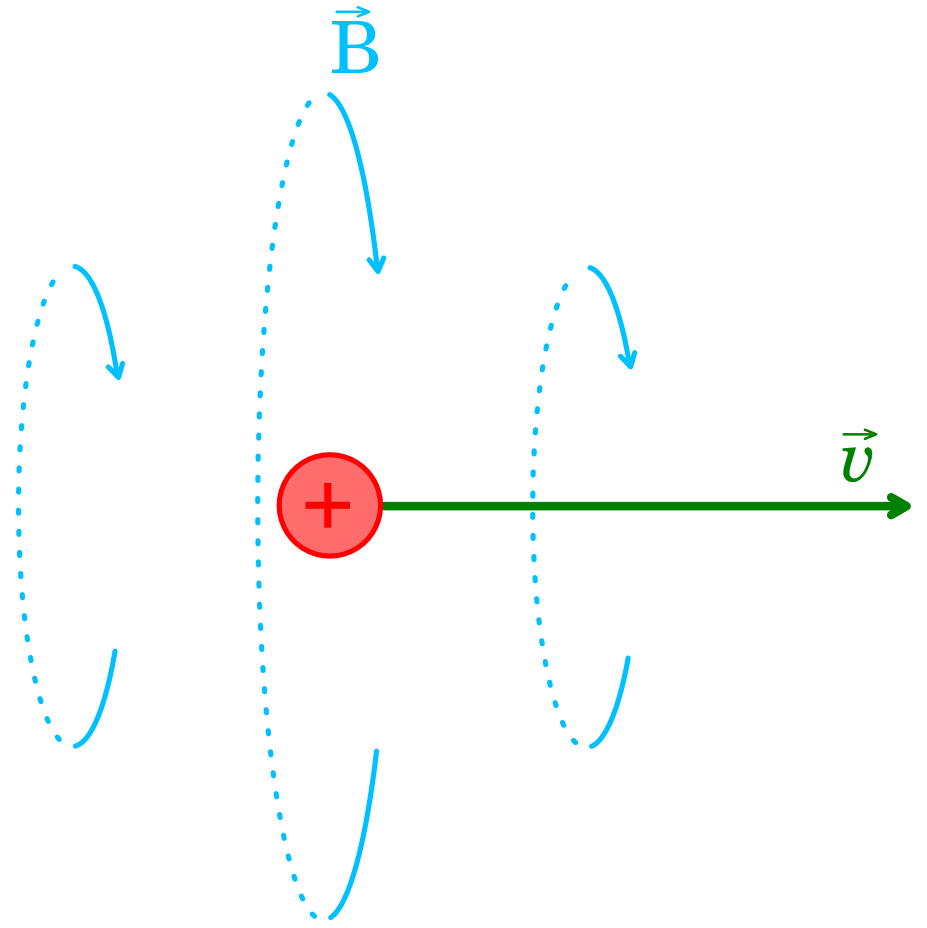
\includegraphics[width=0.3\textwidth]{squematic_charge_magnetic_field.png}
  \caption{Líneas de campo magnético de la carga puntual.}
  \label{fig:lineas_de_campo_magnético_de_la_carga_puntual}
\end{figure}

El campo magnético \(\vec{B}\) generado por la carga puntual \(q\) que se mueve con velocidad constante \(\vec{v}\) en \textbf{un punto del espacio} \(\vec{r}\) está dado por:

\begin{equation}
  \vec{B} = \frac{\mu_0}{4\pi} \frac{q \, \vec{v} \times \hat{r}}{r^2}
  \label{eq:campo_magnético_de_una_carga_puntual}
\end{equation}
donde:
\begin{itemize}
  \item \(\mu_0 = 4 \pi \times 10^{-7} \, \frac{\si{\newton}}{\si{\ampere\squared}}\) es la permeabilidad del vacío,
  \item \(\vec{r}\) es el vector que apunta desde la posición de la carga al punto donde se evalúa el campo,
  \item \(r = |\vec{r}|\) es la magnitud del vector \(\vec{r}\),
  \item \(\hat{r} = \frac{\vec{r}}{r}\) es el vector unitario en la dirección de \(\vec{r}\).
\end{itemize}

\begin{wrapfigure}{r}{0.3\textwidth}
  \centering
  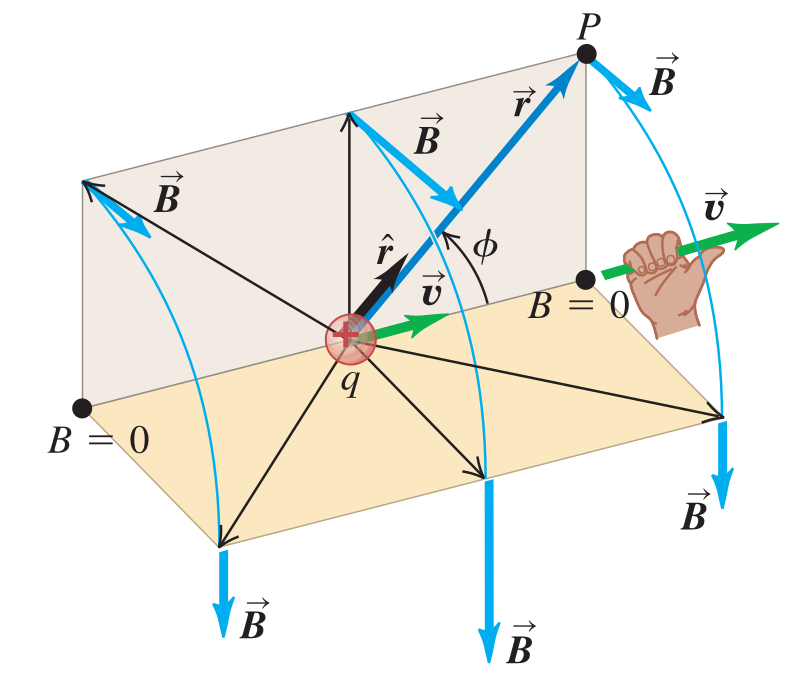
\includegraphics[width=\linewidth]{magnetic_field_of_a_point_charge.png}
  \caption{Campo magnético de una carga puntual.}
  \label{fig:campo_magnético_de_una_carga_puntual}
\end{wrapfigure}
La forma del campo magnético generado por \(q\) es circular, y \(\vec{B}\) es perpendicular a \(\vec{v}\) y \(\vec{r}\). Como se muestra en la figura \ref{fig:campo_magnético_de_una_carga_puntual} el campo magnético \(\vec{B}\) decrece con la distancia al punto \(P\). Además mientras menor es el ángulo entre \(\vec{v}\) y \(\vec{r}\) menor será el campo magnético \(\vec{B}\), y en el caso particular de \(\theta = 0^\circ\) el campo magnético \(\vec{B}\) será cero. 

Este campo magnético es el responsable de que las cargas en movimiento experimenten una fuerza magnética \(\vec{F}_B = q\vec{v} \times \vec{B}\).

Es importante recordar que \textbf{las líneas de campo magnético siempre son cerradas}. Esto lo vimos en la sección \ref{sec:flujo_magnético}, si encerramos un imán en una superficie Gaussiana, todas las líneas de campo magnético que salen, vuelven a entrar. Esto resulta en un flujo nulo.

\begin{tcolorbox}[myconclusion]
  El campo magnético total generado por varias cargas en movimiento es la suma vectorial de los campos generados por las cargas individuales.
\end{tcolorbox}

Con esto en mente, podemos encontrar el campo magnético generado por un diferencial de carga. De la sección \ref{sec:movimiento_de_cargas} sabemos que para un pedacito de segmento de longitud \(dl\) la carga es:
\[
dq = nqA\, dl
\]

De la ecuación \ref{eq:campo_magnético_de_una_carga_puntual} podemos aplicar la definición geométrica del producto vectorial, y reemplazar la carga por la expresión anterior. Entonces el campo magnético \(dB\) generado por un diferencial de carga es:
\begin{align*}
  dB &= \frac{\mu_0}{4\pi} \frac{dq \, v_d \, \sin\theta}{r^2} \\
  dB &= \frac{\mu_0}{4\pi} \frac{\left(nq v_d A\right) dl}{r^2} \sin\theta \\ 
  dB &= \frac{\mu_0}{4\pi} \frac{I dl}{r^2} \sin\theta 
\end{align*}

Entonces el un diferencial de campo magnético \(d\vec{B}\) generado por una corriente \(I\) que fluye a través de un pequeño segmento \(dl\) es:
\begin{equation}
  \boxed{d\vec{B} = \frac{\mu_0}{4\pi} \frac{I \, d\vec{l} \times \hat{r}}{r^2}}
  \label{eq:campo_magnetico_de_un_diferencial_de_corriente}
\end{equation}

\subsubsection{Ley de Biot-Savart}

La fórmula \ref{eq:campo_magnético_de_una_carga_puntual} es una versión simplificada de la Ley de Biot-Savart para una carga puntual. A partir de \eqref{eq:campo_magnetico_de_un_diferencial_de_corriente} podemos obtener la Ley de Biot-Savart que establece que el campo magnético \(\vec{B}\) generado por una corriente \(I\) que fluye a través de una curva \(C\) es:

\begin{equation}
  \vec{B} = \frac{\mu_0}{4\pi} \int_C \frac{I \, \vec{dl} \times \hat{r}}{r^2},
\end{equation}
donde:
\begin{itemize}
  \item \(\mu_0 = 4 \pi \times 10^{-7} \, \frac{\si{\newton}}{\si{\ampere\squared}}\) es la permeabilidad del vacío,
  \item \(\vec{dl}\) es el vector diferencial de longitud de la curva \(C\),
  \item \(r = |\vec{r}|\) es la magnitud del vector \(\vec{r}\),
  \item \(\hat{r} = \frac{\vec{r}}{r}\) es el vector unitario en la dirección de \(\vec{r}\).
\end{itemize}

\subsubsection{Aplicación de la ley de Biot-Savart}
\label{sec:aplicacion_de_la_ley_de_biot_savart}

La ley de Biot-Savart es una ecuación general que describe el campo magnético generado por una corriente. Sin embargo, en la práctica, su aplicación puede ser compleja, especialmente cuando se trata de curvas complejas o cuando se requiere resolver integrales complejas.

En la aplicación práctica de la ley de Biot-Savart, es común simplificar la integración considerando curvas rectas o cilíndricas, lo que permite resolver integrales más simples. Incluso es posible determinar la dirección del campo magnético con la regla de la mano derecha y calcular únicamente el módulo del campo magnético. A continuación se dan los resultados de algunos de los casos más comunes.

Para un segmento largo y recto de cable el módulo del campo magnético se convierte en:
\begin{equation*}
  B = \frac{\mu_0 I}{2\pi r}
\end{equation*}
donde:
\begin{itemize}
  \item \(\mu_0 = 4 \pi \times 10^{-7}\) es la permeabilidad del vacío,
  \item \(I\) es la corriente que fluye a través del cable,
  \item \(r\) es la distancia desde el cable al punto donde se evalúa el campo magnético.
\end{itemize}

\noindent Para una espira circular de radio \(R\) el módulo del campo magnético en el centro es:
\begin{equation*}
  B = \frac{\mu_0 I}{2R}
\end{equation*}

\noindent Para un conjunto de \(N\) espiras de radio \(R\) el campo en el centro es:
\begin{equation*}
  B = \mu_0 \frac{N I}{2R}
\end{equation*}
Este resultado se refiere a \(N\) espiras circulares (o una bobina plana) de radio \(R\), todas concentradas en el mismo plano y con el mismo centro.

\subsubsection{Ley de Ampère}

Hasta el momento, el cálculo del \hl{campo magnético} generado por una corriente ha sido realizado a través de la Ley de Biot-Savart. Sin embargo, esta ley no es la única ecuación que describe el campo magnético generado por una corriente. La Ley de Ampère es una de las ecuaciones fundamentales del electromagnetismo y establece una relación entre el campo magnético \(\vec{B}\) y las corrientes eléctricas que lo generan. 

La Ley de Ampère puede parecer abstracta al principio, pero su lógica es similar a la Ley de Gauss, aunque aplicada al magnetismo. Esta ley establece una relación entre el campo magnético \(\vec{B}\) y las corrientes eléctricas que lo generan. 
\[
\oint_{\text{lazo cerrado}} \vec{B} \cdot d\vec{l} = \mu_0 \, I_{\text{enc}}
\]
donde:
\begin{itemize}
  \item \(\vec{B}\): Campo magnético.
  \item \(d\vec{l}\): Elemento infinitesimal de un camino cerrado (lazo).
  \item \(I_{\text{enc}}\): Corriente neta encerrada por el lazo.
  \item \(\mu_0\): Permeabilidad magnética del vacío (\(4\pi \times 10^{-7} \, \mathrm{T \cdot m/A}\)).
\end{itemize}

\begin{tcolorbox}[myconclusion]
\textbf{¿Sobre qué se integra?}

En la Ley de Ampère, no se integra sobre una superficie, sino sobre un camino cerrado (lazo o bucle). Este camino cerrado se llama lazo amperiano, y es análogo a la superficie gaussiana en la Ley de Gauss, pero con diferencias importantes:
\begin{itemize}
  \item Ley de Gauss: Integral sobre una superficie cerrada.
  \subitem Relaciona el flujo eléctrico (\(\oint \vec{E} \cdot d\vec{A}\)) con la carga encerrada.  
  \item Ley de Ampère: Integral sobre un camino cerrado (una línea).
  \subitem Relaciona la circulación del campo magnético (\(\oint \vec{B} \cdot d\vec{l}\)) con la corriente encerrada.  
\end{itemize}
\end{tcolorbox}

Un camino amperiano es un camino imaginario cerrado que tú defines, al igual que la superficie gaussiana. Debe elegirse estratégicamente para aprovechar la simetría del problema (por ejemplo, círculos concéntricos alrededor de un alambre recto). 

\paragraph{¿Qué representa la integral \(\oint \vec{B} \cdot d\vec{l}\)?}

La integral \(\oint \vec{B} \cdot d\vec{l}\) se llama circulación del campo magnético y representa la suma de las componentes tangenciales de \(\vec{B}\) a lo largo del lazo amperiano. En términos físicos:
\[
\oint \vec{B} \cdot d\vec{l} = \mu_0 \, I_{\text{enc}}
\]
\begin{itemize}
  \item Lado izquierdo: Circulación del campo magnético (¿cómo ``rota'' \(\vec{B}\) alrededor del lazo?).  
  \item Lado derecho: Corriente total de conducción que atraviesa la superficie encerrada por el lazo.  
\end{itemize}

\paragraph{¿Qué buscamos con la Ley de Ampère?}

El objetivo principal es calcular el \textbf{campo magnético} (\(\vec{B}\)) en situaciones con alta simetría, donde la integral \(\oint \vec{B} \cdot d\vec{l}\) se simplifica. Por ejemplo: En un alambre infinito, un solenoide, o un toroide.  

\begin{itemize}
  \item Alambre infinito recto:  
    \[
    B = \frac{\mu_0 I}{2\pi r} \quad \text{(dirección circular alrededor del alambre)}.
    \]
  \item Solenoide ideal:  
     \[
     B = \mu_0 n I \quad \text{(campo uniforme en el interior)}.
     \]
  \item Toroide:  
     \[
     B = \frac{\mu_0 N I}{2\pi r} \quad \text{(campo circular dentro del toroide)}.
     \]
\end{itemize}
Nótese que los resultados son consistentes con la Ley de Biot-Savart. Para el alambre infinito (o largo) y recto se ha obtenido el mismo resultado. Aunque usted tal vez se pregunte ¿Qué paso con el solenoide ideal? Parece que no ha dado lo mismo que el ejemplo del conjunto de espiras. Esto es porque el solenoide tiene la forma de un cilindro, como se vió en la figura \ref{fig:solenoide}. Un solenoide es una bobina alargada con \(N\) espiras distribuidas uniformemente a lo largo de una longitud \(L\). El ejemplo de las espiras en la sección \ref{sec:aplicacion_de_la_ley_de_biot_savart} es un conjunto de espiras que no tiene forma de cilindro, sinó que están todas en el mismo plano.

\paragraph{Ejemplo práctico: Cálculo del campo magnético en un solenoide}

Consideremos un solenoide de \(N\) vueltas, longitud \(L\), y corriente \(I\):

\textbf{Definimos el lazo amperiano}: Rectángulo que abarca parte del solenoide.

\textbf{Aplicación de Ampère}: 
\[
  \oint \vec{B} \cdot d\vec{l} = B \cdot L_{\text{interior}} = \mu_0 n I L_{\text{interior}},
\]
donde \(n = N/L\) (vueltas por unidad de longitud).  

\textbf{Resultado}: 
\[
  B = \mu_0 n I.
\]
\section{Movimiento Ondulatorio}

Antes de comenzar con el movimiento ondulatorio te recomiendo que revises el resumen de movimiento armónico simple en la sección \ref{sec:mas}. El movimiento ondulatorio está estrechamente relacionado con el movimiento armónico simple.

Un movimiento ondulatorio es un movimiento que se caracteriza por la transferencia de energía a través del espacio sin el acompañamiento de transferencia de materia. Todas las ondas mecánicas requieren:
\begin{enumerate}
  \item alguna fuente de perturbación
  \item un medio que contenga elementos que puedan ser perturbados y
  \item algún mecanismo físico a partir del cual los elementos del medio puedan influirse mutuamente.
\end{enumerate}

\begin{wrapfigure}{r}{0.3\textwidth}
  \centering
  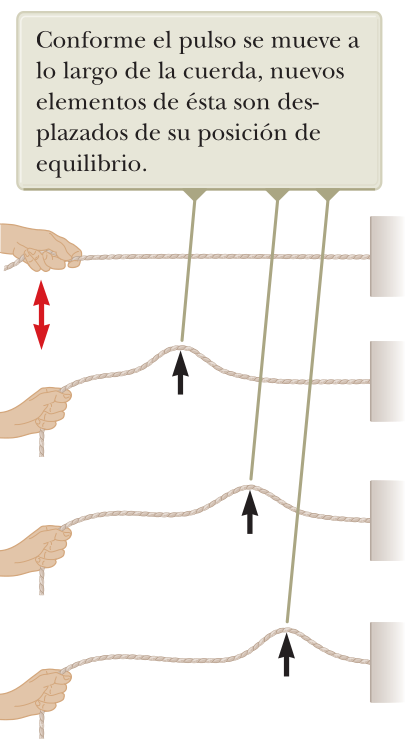
\includegraphics[width=\linewidth]{wave_example.png}
  \caption{Un pulso que viaja a lo largo de la cuerda.}
  \label{fig:wave_example}
\end{wrapfigure}
La onda \textbf{es una perturbación} que experimenta el sistema y que lo aparta de su posición de equilibrio. Una \textit{onda} es un tren de pulsos, es decir, muchos pulsos periódicos (o bien, pulsos iguales seguidos separados uniformemente entre sí).

Por ejemplo, si se observa la figura \ref{fig:wave_example}, una mano mueve una vez, hacia arriba y hacia abajo, el extremo de una cuerda estirada, generando un \textit{pulso} que viaja a lo largo de la cuerda con una rapidez definida. La mano en este caso se denomina \textbf{foco de onda} que es el punto o región desde la cual se origina o se concentra la propagación de la onda.

Lo que se transmite a través de la cuerda, a cada punto cercano, es \textbf{energía, no materia}. Es decir, las partículas que conforman la cuerda no se desplazan a la derecha, sino más bien, se mueven hacia arriba y hacia abajo, y lo que se desplaza a la derecha es el pulso. Las ondas formadas por este tipo de pulso, donde el movimiento de las partículas es \hl{\textit{perpendicular}} a la dirección de propagación del pulso se denominan \textbf{ondas transversales}.

Hay otro tipo de propagación de onda. Aquella onda cuya propagación es \hl{\textit{paralela}} a la perturbación provocada por el pulso se denomina \textbf{onda longitudinal}. Se puede comparar el pulso de onda \textbf{transversal} de la figura \ref{fig:wave_example} con el pulso de onda \textbf{longitudinal} de la figura \ref{fig:longitudinal_wave}.

\begin{figure}[ht]
  \centering
  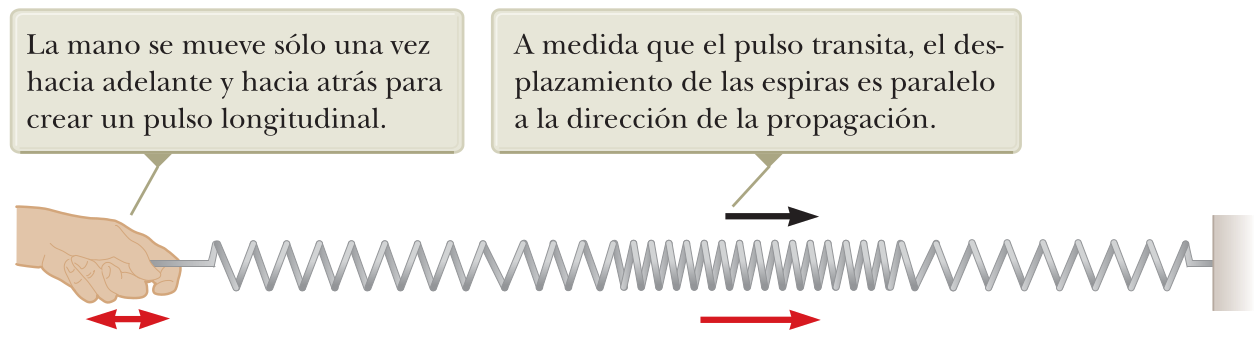
\includegraphics[width=0.8\textwidth]{logitudinal_wave.png}
  \caption{Un pulso que viaja a lo largo de un resorte.}
  \label{fig:longitudinal_wave}
\end{figure}

Para poder poner en movimiento estos medios en los que se propagan las ondas hay que \hl{aportar energía} al sistema realizando trabajo mecánico sobre el mismo. La onda es el transporte de energía de una región del medio a otra. Esa energía cuando llega a cualquier punto del medio, lo aparta de su posición de equilibrio, poniéndolo a vibrar. 

\subsection{Análisis de modelo de onda}

Si tomamos el ejemplo de la cuerda, pero ahora en vez de generar un pulso generamos un tren de pulsos como se muestra en la figura \ref{fig:wave_train} sabemos que la onda será transversal y también que las partículas que conforman la cuerda vibran con un movimiento armónico simple. De ahí podemos definir algunas cantidades importantes.

\begin{figure}[ht]
  \centering
  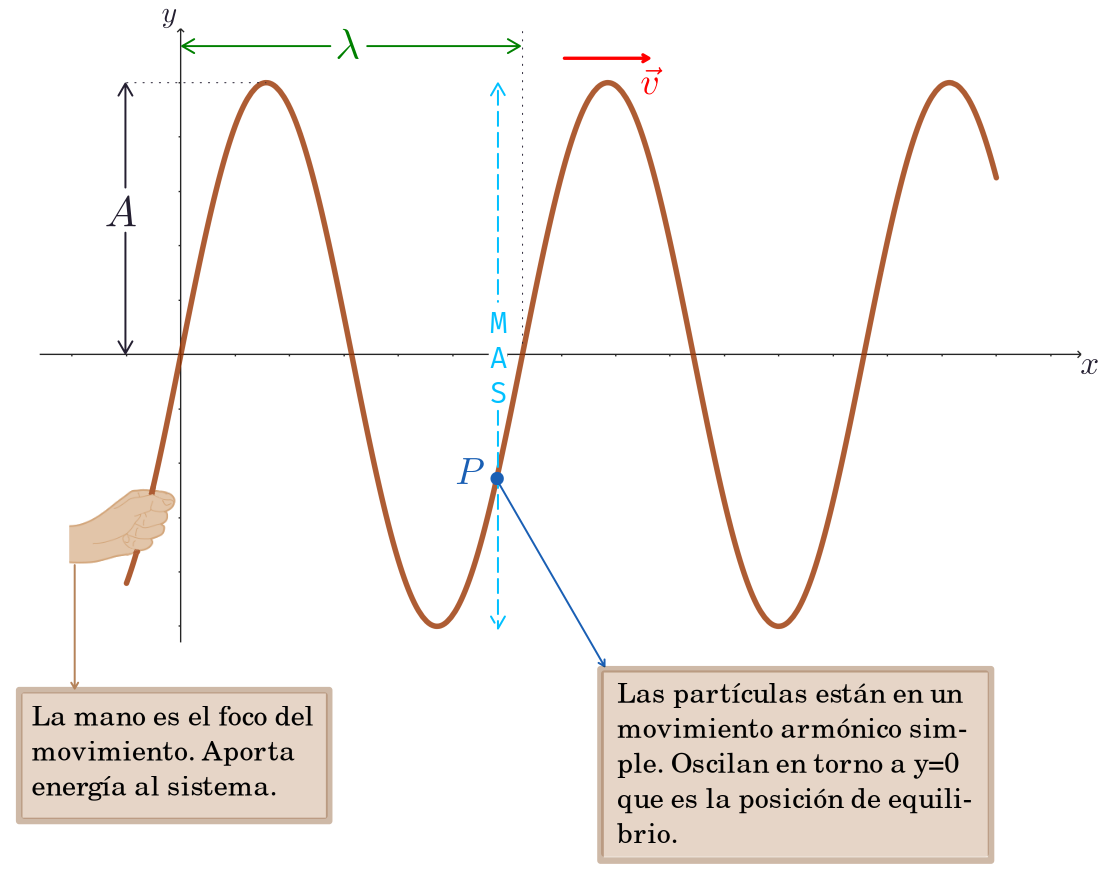
\includegraphics[width=0.8\textwidth]{wave_train.png}
  \caption{Un tren de pulsos que viajan a lo largo de la cuerda.}
  \label{fig:wave_train}
\end{figure}

A continuación te presento las \textit{cantidades físicas básicas} que caracterizan a una onda armónica, junto con su definición, unidad en el SI y su relación con otras magnitudes.

\subsubsection{Cantidades físicas básicas de una onda}
\label{sec:waves_basic_quantities}

\paragraph{Amplitud (\(A\))}

Es el valor máximo que alcanza la magnitud oscilante respecto de su posición de equilibrio.

\begin{itemize}
  \item Unidad: depende del tipo de onda, en el caso de ondas mecánicas su unidad es metros (\(\si{\meter}\)).
  \item Interpretación: indica la intensidad o energía de la onda.
  \item No afecta la velocidad, pero sí la energía transportada.
\end{itemize}

\paragraph{Período (\(T\))}

Es el tiempo que tarda un punto del medio en realizar una oscilación completa. Si vemos la figura \ref{fig:wave_train} el punto \(P\) está en un movimiento armónico simple. Una oscilación completa demora \(T\) segundos, que es un período. 

\begin{itemize}
  \item Unidad: segundos (s).
  \item Relación: inversamente proporcional a la frecuencia: \(T = \frac{1}{f}\)
\end{itemize}

\paragraph{Frecuencia (\(f\))}

Es el número de oscilaciones completas por unidad de tiempo.

\begin{itemize}
  \item Unidad: hertz (Hz), donde \(1\, \text{Hz} = 1\, \text{oscilación/s}\).
  \item Relación: \(f = \frac{1}{T}\)
\end{itemize}

\paragraph{Longitud de onda (\(\lambda\))}

Es la distancia entre dos puntos consecutivos que están en la misma fase (por ejemplo, dos crestas sucesivas). Como se ve en la figura \ref{fig:wave_train} la longitud de onda es la distancia entre dos puntos en fase. 

En una onda mecánica, dos puntos están en fase cuando cumplen las siguientes condiciones:

\begin{enumerate}
  \item Tienen el mismo estado de vibración en el mismo instante, es decir:
    \begin{itemize}
      \item Mismo desplazamiento (posición) respecto a la posición de equilibrio.
      \item Misma velocidad (moviéndose en la misma dirección).
      \item Misma aceleración.
    \end{itemize}
  \item La diferencia de fase entre ellos es un múltiplo entero de \(2\pi\) radianes (o \(0\), \(\pm 2\pi\), \(\pm 4\pi\), etc.). 
  \item La distancia entre ellos es un múltiplo entero de la longitud de onda (\(\lambda\)):
   \[
   \Delta x = n\lambda \quad \text{(con \(n = 0, \pm 1, \pm 2, \dots\))}
   \]
\end{enumerate}

Si la diferencia de fase es \(\pi\) radianes (o un múltiplo impar de \(\pi\)), los puntos están en \textbf{oposición de fase} (máximo alejamiento en vibración). Dos puntos están en fase cuando su separación espacial es un múltiplo entero de \(\lambda\) y su diferencia de fase es \(2\pi n\). Esto implica que oscilan sincronizados.

\begin{itemize}
  \item Unidad: metros (m).
  \item Relación: \(\lambda = \frac{v}{f} = v T\)
\end{itemize}

\paragraph{Velocidad de propagación (\(v\))}

Es la velocidad con que se desplaza el frente de onda (es decir, cómo se propaga la perturbación en el medio).

\begin{itemize}
  \item Unidad: metros por segundo (m/s).
  \item Relación fundamental: la velocidad de propagación de una onda es \(v = \lambda f\)
\end{itemize}

La velocidad de propagación depende del medio en el que se propaga la onda. Por ejemplo, la velocidad de propagación de una onda sonora en el aire es de \(343\, \text{m/s}\) a temperatura ambiente. En la materia Física II se trabaja principalmente con la velociad de propagación en un alambre o cuerda fina. 

La velocidad de propagación de una onda en una cuerda tensa indica con qué rapidez se traslada la perturbación (o energía) a lo largo de la cuerda. Esta velocidad depende exclusivamente de las propiedades físicas del medio, es decir, de la tensión aplicada a la cuerda y de su densidad lineal de masa.

La velocidad \(v\) de propagación de una onda transversal en una cuerda idealmente elástica y tensa se calcula mediante la siguiente fórmula:
\[
v = \sqrt{\frac{T}{\mu}}
\]
donde:
\begin{itemize}
  \item \(T\) es la tensión en la cuerda (en newtons, N),
  \item \(\mu\) es la densidad lineal de masa de la cuerda, es decir, la masa por unidad de longitud (en kg/m).
\end{itemize}

Cuanto mayor es la tensión \(T\) en la cuerda, más rápidamente se propaga la onda. Esto es porque la fuerza que ``restaura'' la cuerda hacia su equilibrio es mayor, lo que permite transmitir la perturbación más eficazmente.

Cuanto mayor es la densidad lineal \(\mu\) (es decir, cuanto más pesada es la cuerda por unidad de longitud), más difícil es acelerar sus partículas, lo que reduce la velocidad de propagación.

A nivel conceptual, se puede entender la fórmula considerando un pequeño elemento de cuerda \(\mu \, \mathrm{d}x\), este pequeño elemento de masa está sometido a fuerzas de tensión desde los extremos. Aplicando la segunda ley de Newton al análisis de estas fuerzas y a la aceleración transversal que experimenta el segmento debido a la curvatura local de la cuerda, se obtiene una ecuación de onda. Esta ecuación predice una velocidad de propagación que resulta ser \(v = \sqrt{T / \mu}\).

\paragraph{Número de onda (\(k\))}

Es una medida del número de ciclos por unidad de longitud, análogo espacial de la frecuencia temporal.

\begin{itemize}
  \item Unidad: radianes por metro (rad/m).
  \item Relación: \(k = \frac{2\pi}{\lambda}\)
\end{itemize}

\paragraph{Frecuencia angular (\(\omega\))}

Es la frecuencia expresada en términos angulares (radianes por segundo).

\begin{itemize}
  \item Unidad: rad/s.
  \item Relación: \(\omega = 2\pi f = \frac{2\pi}{T}\)
\end{itemize}

\paragraph{Fase (\(\vartheta\)) y diferencia de fase}

La fase indica en qué punto del ciclo se encuentra la oscilación. Es el mismo concepto de fase que se encuentra en el movimiento armónico simple. Si no lo recuerdas te recomiendo que revises el capítulo \ref{sec:mas}.

Estas cantidades permiten construir la función de onda general de una onda armónica:
\[
y(x, t) = A \cos(kx - \omega t + \varphi)
\]
La deducción de la ecuación de onda la veremos más adelante, por ahora te recomiendo que simplemente la recuerdes y prestes atención al concepto de fase que no requiere que sepas cómo se deduce.

En esta ecuación la fase \(\vartheta\) (variable theta) es el argumento del coseno, es decir \(\vartheta = kx - \omega t + \varphi\). Esta cantidad no tiene unidades, y se mide en radianes. La fase describe en qué punto del ciclo se encuentra la onda en un lugar y momento dados. Dos puntos de la onda que tengan el mismo valor de fase están en la misma etapa del ciclo: por ejemplo, ambos en una cresta o ambos en un nodo.

La diferencia de fase es la distancia angular (en radianes) entre dos ondas o entre dos puntos de una misma onda. Se denota típicamente como \(\Delta \varphi\) o simplemente \(\delta\). En general hay dos contextos donde se habla de diferencia de fase:
\begin{enumerate}
  \item Entre dos ondas distintas
  \item Entre dos puntos de una misma onda
\end{enumerate}

Veamos el primer caso. Supongamos dos ondas con igual frecuencia y número de onda:
\[
\psi_1(x,t) = A \cos(kx - \omega t) \\
\psi_2(x,t) = A \cos(kx - \omega t + \delta)
\]
Entonces, la diferencia de fase entre ambas es \(\delta\). Esto determina si las ondas están en fase (cuando \(\delta = 0\) o múltiplos de \(2\pi\)) o desfasadas (por ejemplo, \(\delta = \pi\) implica interferencia destructiva).

Para el segundo caso la diferencia de fase entre dos posiciones fijas \(x_1\) y \(x_2\) en un instante dado es:
\[
\Delta \theta = k(x_2 - x_1)
\]
Esto se puede expresar como:
\[
\Delta \theta = \frac{2\pi}{\lambda} (x_2 - x_1)
\]
Por lo tanto, dos puntos separados por una longitud de onda completa tienen una diferencia de fase de \(2\pi\) radianes, es decir, están en fase.

Entonces, resumiendo los conceptos tendríamos:
\begin{itemize}
  \item Si dos ondas están en fase, sus crestas y valles coinciden, y se refuerzan al superponerse (interferencia constructiva).
  \item Si están en oposición de fase ($\Delta \varphi = \pi$), las crestas de una coinciden con los valles de la otra (interferencia destructiva).
  \item En sistemas oscilatorios (como masas o circuitos), la fase también indica el retraso temporal entre dos oscilaciones.
\end{itemize}

\subsubsection{Frente de ondas}

El frente de onda es el lugar geométrico de los puntos del medio que están en la misma fase de oscilación en un instante determinado. En otras palabras, es el conjunto de puntos donde la magnitud de la onda (como el desplazamiento) tiene el mismo valor y evolución temporal dentro del ciclo de la onda.

Por ejemplo, en una onda armónica, todos los puntos de un frente de onda alcanzan sus máximos, mínimos y posiciones de equilibrio al mismo tiempo.

El frente de onda proporciona información fundamental sobre la geometría y el comportamiento de la onda. Entre las principales características que define o influye se encuentran:

\paragraph{1. Dirección de propagación}

El frente de onda es \hl{perpendicular} a la dirección en que la energía y la perturbación se propagan. Por lo tanto, la orientación de los frentes determina la dirección del avance de la onda.

\paragraph{2. Forma de la onda}

La geometría del frente de onda determina la naturaleza de la propagación:
\begin{itemize}
  \item Si los frentes son planos, la onda es plana, lo que implica propagación rectilínea desde una fuente lejana o colimada. Las ondas de luz que provienen del sol pueden ser consideradas planas por ejemplo.
  \item Si los frentes son esféricos, la onda se propaga en todas direcciones desde una fuente puntual. El sonido que proviene de un punto fijo en el aire es un ejemplo de onda esférica.
  \item En medios anisótropos o con obstáculos, los frentes pueden deformarse, generando fenómenos como difracción o focalización.
\end{itemize}

\paragraph{3. Interacción con el medio}

La forma y evolución de los frentes de onda permite estudiar fenómenos como:
    \begin{itemize}
      \item Reflexión: el frente se repliega sobre sí mismo al encontrar una barrera.
      \item Refracción: el frente cambia de dirección y velocidad al pasar a otro medio.
      \item Difracción: el frente se curva al atravesar rendijas o bordes.
      \item Interferencia: superposición de frentes de onda de diferentes fuentes.
    \end{itemize}

\paragraph{4. Velocidad de propagación}

La separación temporal entre frentes consecutivos (por ejemplo, entre dos crestas en el tiempo) y la distancia espacial entre ellos (la longitud de onda) permiten calcular la velocidad de propagación de la onda.

\subsection{Deducción de la ecuación de onda}

El movimiento ondulatorio supone la transmisión de una perturbación a través de un punto a otro sin transporte de materia. Nuestro objetivo es encontrar una ecuación matemática que permita conocer el estado de vibración de cada punto a medida que transcurre el tiempo.

\begin{wrapfigure}{r}{0.3\textwidth}
  \centering
  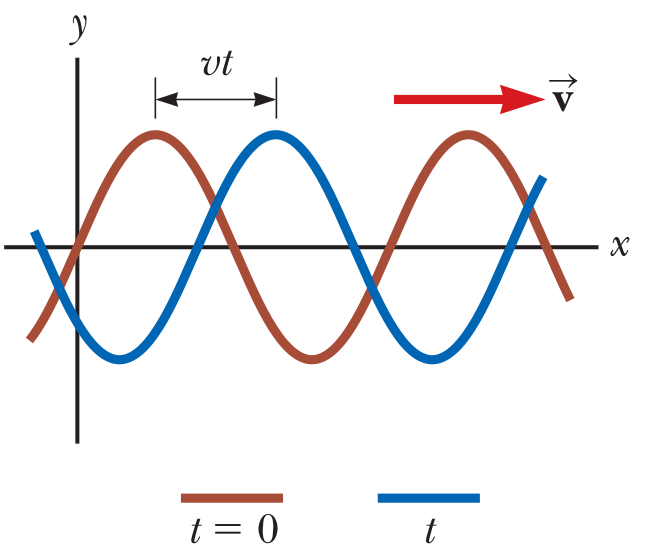
\includegraphics[width=\linewidth]{sin_wave.png}
  \caption{Onda sinusoidal que viaja hacia la derecha con una rapidez \(v\).}
  \label{fig:sin_wave}
\end{wrapfigure}
Para no complicar las cosas, continuemos con el ejemplo de la cuerda. Supongamos que la cuerda tiene un movimiento ondulatorio, y como ya hemos visto, la perturbación en la cuerda crea ondas transversales, y sinusoidales en este caso. 

La onda de color marrón de la figura \ref{fig:sin_wave} describe el estado inicial de la cuerda, es decir, es una instantánea de la onda sinusoidal en \(t=0\). Por otro lado la onda de color azul representa una instantánea de la misma cuerda en algún tiempo posterior \(t\), que llamaremos \(t_1\) para evitar confusión (aunque no se muestra en la figura).

Enfoquemos nuestra atención en un solo pulso de la onda. Si comparamos las instantáneas de la cuerda en \(t=0\) y \(t=t_1\), vemos que el pulso ha viajado una distancia \(v t_1\), donde \(v\) es la velocidad de propagación de la onda. 

Analizando el gráfico vemos que pueden ocurrir dos tipos de movimiento al mismo tiempo:
\begin{itemize}
  \item \textbf{El movimiento de la onda}: ya que la curva marrón, después de que transcurra el tiempo \(t\) llegará a la posición de la curva azul.
  \item \textbf{El movimiento de los elementos del medio}: se mueven de arriba a abajo con un \textit{movimiento armónico simple}. 
\end{itemize}

Si fijamos un tiempo determinado como \(t=0\), como el movimiento que describe la posición de los elementos del medio es un movimiento armónico simple, podemos describir la posición vertical de cada elemento del medio según su posición horizontal con la ecuación:
\begin{equation}
  y(x, t=0) = A \sin(ax)
  \label{eq:sin_wave}
\end{equation}
donde \(A\) es la amplitud, \(a\) es una constante a determinar y \(x\) es la posición horizontal. 

De la ecuación \ref{eq:sin_wave} entonces, se ve que si \(x=0\) entonces \(y=0\), lo que coincide con la figura \ref{fig:sin_wave} en \(t=0\). El siguiente valor de \(x\) para el que \(y\) es cero es \(x=\lambda/2\) como se ve en la figura \ref{fig:sin_wave_2}

Por lo tanto, en base a estas observaciones, podemos escribir:
\[
  y(\lambda/2, t=0) = A \sin(a\lambda/2) = 0
\]
  
\begin{wrapfigure}{l}{0.35\textwidth}
  \centering
  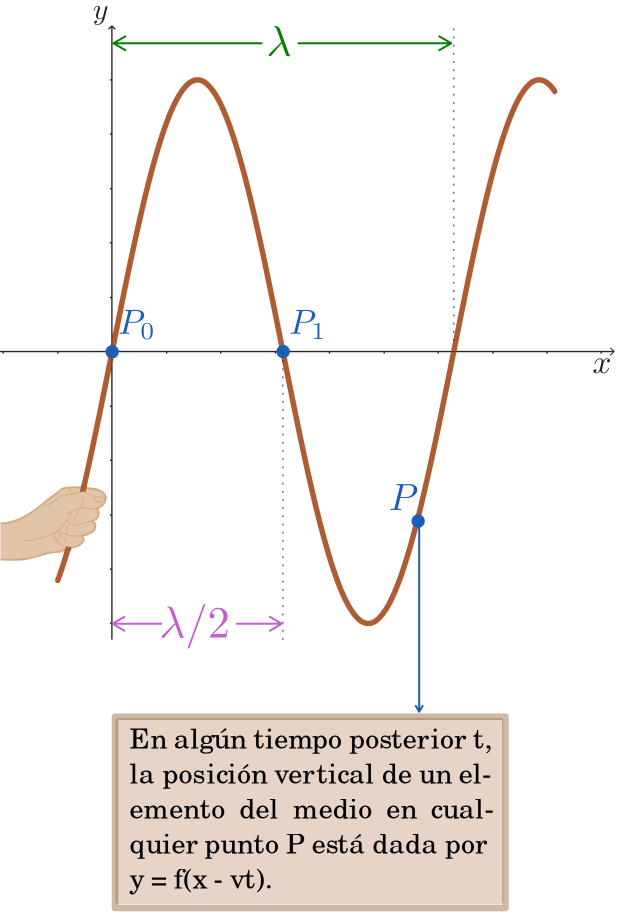
\includegraphics[width=\linewidth]{sin_wave_2.png}
  \caption{Instantánea de la cuerda en \(t=0\) donde una partícula \(P\) cualquiera tiene la misma posición vertical que \(P_0\) cuando la onda viaja una distancia \(v t\).}
  \label{fig:sin_wave_2}
\end{wrapfigure}
Para que esta ecuación sea cierta debe tener \(a\lambda/2 = \pi\) o \(a\lambda/2 = 2\pi\) (en base a la figura \ref{fig:sin_wave_2}), ya que estas posiciones están en fase. En consecuencia, la función que describe las posiciones de todos los elementos del medio a través del que viaja la onda sinusoidal para el instante \(t=0\) se puede escribir como:
\[
  y(x, t=0) = A \sin(\frac{2\pi}{\lambda} x) = 0
\]

Observe que la posición vertical de un elemento del medio es la misma simepre que \(x\) aumente un multiplo entero de \(\lambda\).

Como un pulso de la onda viaja a una velocidad constante \(v\), un elemento cualquiera \(P\) de la cuerda tendrá la misma posición vertical que \(P_0\) en el instante \(t_0\) cuando transcurra un tiempo \(t\) y el pulso de la onda viaje una distancia \(v t\). Entonces, en general podemos expresar la posición de cualquier elemento para todas las posiciones y tiempos como \(f(x - v t)\) donde \(f\) es una función periodica. En este caso \(f\) es la función seno, por lo que resulta:
\[
  y(x, t) = A \sin\left(\frac{2\pi}{\lambda} (x - v t)\right)
\]
  
Sabemos que \(v = \lambda / T ~~ \rightarrow ~~ T = \lambda/v\), por lo que si operamos la ecuación anterior obtenemos:
\begin{align*}
  y(x, t) & = A \sin\left[2\pi \left(\frac{x}{\lambda} - \frac{vt}{\lambda} \right)\right] \\
  y(x, t) & = A \sin\left[2\pi \left(\frac{x}{\lambda} - \frac{t}{T} \right)\right]
\end{align*}

Y recordando las cantidades básicas definidas en la sección \ref{sec:waves_basic_quantities}, podemos escribir:

\begin{equation}
  \boxed{y(x,t) = A \sin(kx - \omega t + \varphi)}
\end{equation}
\begin{itemize}
  \item \(kx\) representa el cambio de fase con la posición (espacial),
  \item \(\omega\) representa el cambio de fase con el tiempo (temporal),
  \item \(\varphi\) es la fase inicial, que determina el estado de oscilación en el origen espacial y temporal.
\end{itemize}

\subsection{Energía asociada al movimiento ondulatorio}

La energía asociada al movimiento ondulatorio en ondas mecánicas proviene del hecho de que cada partícula del medio oscila en torno a su posición de equilibrio debido a la acción de una perturbación. Esta oscilación implica que hay energía almacenada en el medio, tanto en forma de energía cinética como potencial.

Vamos a continuar el análisis para una onda armónica transversal que se propaga en una cuerda (para continuar con el mismo ejemplo que venimos usando). 

\begin{tcolorbox}[myconclusion]
  Recuerda que la función seno es la misma que la función coseno, pero desplazada \(\pi/2\).
\end{tcolorbox}

Consideramos una onda transversal que se propaga en la dirección \(x\), con desplazamiento en la dirección \(y\), y que \(\varphi = \pi/2\):
\[
y(x,t) = A \sin(kx - \omega t + \pi/2) = \boxed{A \cos(kx - \omega t)}
\]
donde:
\begin{itemize}
  \item \(A\) es la amplitud,
  \item \(\omega\) la frecuencia angular,
  \item \(k\) el número de onda.
\end{itemize}

Cada punto de la cuerda oscila verticalmente con esta función. En base a esta ecuación, podemos calcular la energía cinética y potencial de la cuerda.

\begin{tcolorbox}[myconclusion]
  Hemos supuesto una onda desplazada \(\pi/2\) para demostrar que el signo de la velocidad no influye en el resultado. En realidad, es lo mismo trabajar con coseno que con seno, solo hay que tener la precaución de respetar el desfase en la función dada. Aunque en este caso, como es un ejemplo, la función la hemos inventado.
\end{tcolorbox}

\subsubsection{Energía cinética}

Una partícula de masa \(\mathrm{d}m\) en la cuerda tiene una velocidad vertical dada por su ecuación de M.A.S.:

\[
v_y(x,t) = \frac{\partial y}{\partial t} = -A \omega \sin(kx - \omega t)
\]

La energía cinética diferencial en un instante dado es:
\[
\mathrm{d}E_{\text{cin}} = \frac{1}{2} \, \mathrm{d}m \cdot v_y^2(x,t)
\]

Si la cuerda tiene densidad lineal \(\mu\) (en kg/m), entonces \(\mathrm{d}m = \mu \, \mathrm{d}x\). Por tanto:

\[
\mathrm{d}E_{\text{cin}} = \frac{1}{2} \mu \, A^2 \omega^2 \sin^2(kx - \omega t) \, \mathrm{d}x
\]

\subsubsection{Energía potencial}

La energía potencial elástica proviene de la deformación de la cuerda debido a su curvatura. En una cuerda ideal, se puede demostrar que, para pequeñas oscilaciones, la energía potencial tiene la misma forma media que la energía cinética. Se obtiene:

\[
\mathrm{d}E_{\text{pot}} = \frac{1}{2} \mu \, A^2 \omega^2 \cos^2(kx - \omega t) \, \mathrm{d}x
\]

\subsubsection{Energía total por unidad de longitud}

Sumando ambas contribuciones:

\[
\mathrm{d}E = \mathrm{d}E_{\text{cin}} + \mathrm{d}E_{\text{pot}} = \frac{1}{2} \mu A^2 \omega^2 \left[ \sin^2(kx - \omega t) + \cos^2(kx - \omega t) \right] \mathrm{d}x
\]

Como \(\sin^2 + \cos^2 = 1\), se obtiene la energía total por unidad de longitud:

\[
\frac{\mathrm{d}E}{\mathrm{d}x} = \mu A^2 \omega^2 \cdot \frac{1}{2}
\]


\subsubsection{Interpretación de la energía}

La energía total transportada por la onda es proporcional al cuadrado de la amplitud \(A^2\), la densidad lineal \(\mu\) y al cuadrado de la frecuencia angular \(\omega^2\). Esta energía se transporta a lo largo de la dirección de propagación de la onda, sin que las partículas del medio se desplacen en esa dirección.

\subsubsection{Potencia transportada por la onda}

La potencia media (energía transportada por segundo) es:

\[
P = \frac{\mathrm{d}E}{\mathrm{d}t} = \frac{1}{2} \mu A^2 \omega^2 v
\]

donde \(v\) es la velocidad de propagación de la onda.


\subsection{Intensidad de la onda}

La \textbf{intensidad de una onda} es una magnitud física que mide la energía transportada por unidad de tiempo y por unidad de área perpendicular a la dirección de propagación. En otras palabras, indica cuánta energía atraviesa una determinada superficie en un segundo debido al paso de una onda.

La intensidad \(I\) se define como:

\[
I = \frac{P}{S}
\]
donde:
\begin{itemize}
  \item \(P\) es la potencia transportada por la onda (energía por unidad de tiempo, en vatios),
  \item \(S\) es el área perpendicular a la dirección de propagación (en m²),
  \item \(I\) se expresa en vatios por metro cuadrado: \(\text{W/m}^2\).
\end{itemize}

Como la intensidad ``depende'' de la potencia, podemos deducir algunas características importantes. 

\paragraph{1. Proporcionalidad con la amplitud cuadrada}

La intensidad crece con el cuadrado de la amplitud de la onda (ya que la potencia es proporcional a la amplitud cuadrada):
\[
I \propto A^2
\]
Esto implica que una onda con el doble de amplitud transporta cuatro veces más energía por segundo y por área.

\paragraph{2. Disminución con la distancia}

En medios sin absorción, la intensidad de una onda esférica (como una onda sonora desde una fuente puntual) disminuye con el cuadrado de la distancia:
\[
I(r) = \frac{P}{4\pi r^2}
\]

Este resultado proviene del hecho de que la energía se distribuye sobre una superficie esférica que crece con \(r^2\), de ahí la ley del inverso del cuadrado.
\begin{figure}[ht]
  \centering
  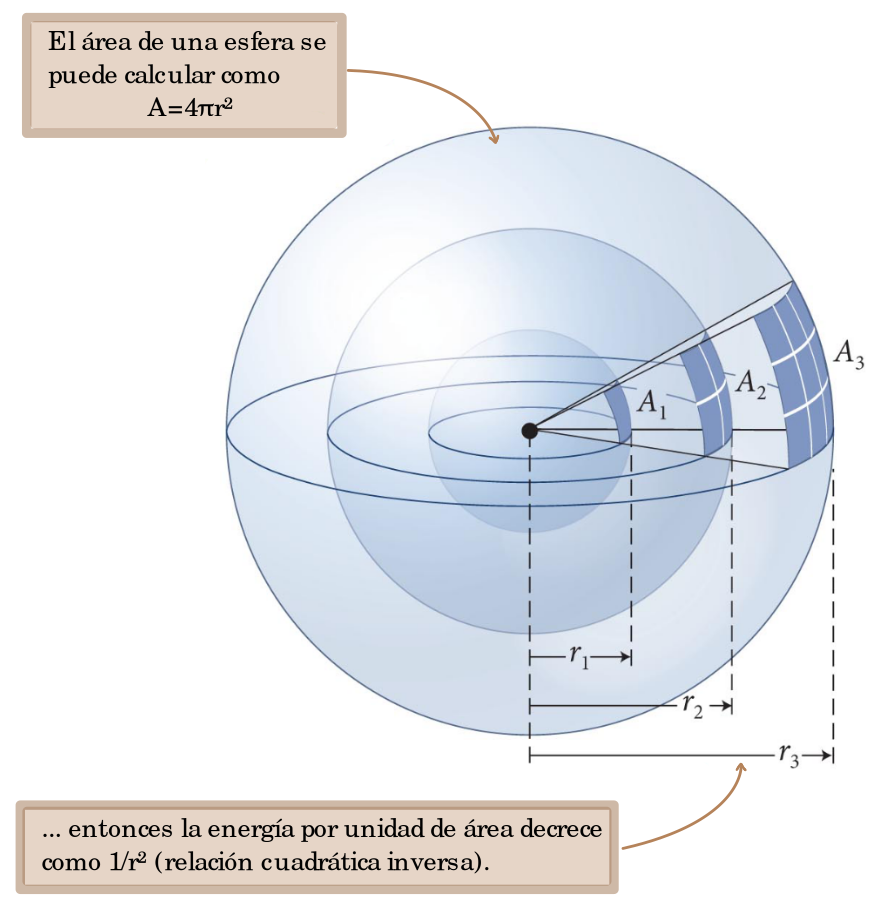
\includegraphics[width=0.6\textwidth]{intensity_decrease.png}
  \caption{Disminución de la intensidad con la distancia en una onda esférica.}
  \label{fig:intensity_decrease}
\end{figure}
Como se ve en la figura \ref{fig:intensity_decrease}, la potencia emitida es constante, sin embargo, a medida que el radio aumenta el área aumenta. Esto significa que la intensidad (es decir la potencia por uniad de área) es menor.

\paragraph{3. Medición directa de energía percibida}

En muchas aplicaciones físicas y técnicas (como en acústica o electromagnetismo), la intensidad está directamente relacionada con la sensación física percibida, como el volumen del sonido o la brillantez de la luz.

La intensidad de una onda cuantifica su capacidad de transportar energía a través del espacio. Es un parámetro fundamental cuando se estudian fenómenos como la absorción, reflexión, interferencia, o cuando se desea conocer el efecto físico de la onda en un sistema receptor.

\section{La luz y su naturaleza dual}
\label{sec:optica}

\subsection{Historia de la luz y sus teorías}

Antes de comenzar con el tema, veamos un breve resumen de la historia de la luz y sus teorías. Esto nos va a servir para saber qué entendemos por luz y por qué no vamos a usar las ecuaciones de onda del capitulo pasado.

\subsubsection{La teoría corpuscular de Newton}

A finales del siglo XVII, Isaac Newton propuso que la luz estaba compuesta por pequeños corpúsculos (partículas). Esta teoría corpuscular explicaba bien la reflexión y la refracción: al considerar que las partículas de luz eran atraídas por los medios más densos, se podía justificar el cambio de dirección (ley de Snell). Newton también contaba con gran autoridad científica, por lo que su modelo prevaleció durante mucho tiempo.

\subsubsection{La teoría ondulatoria de Huygens}

\begin{wrapfigure}{r}{0.25\textwidth}
  \centering
  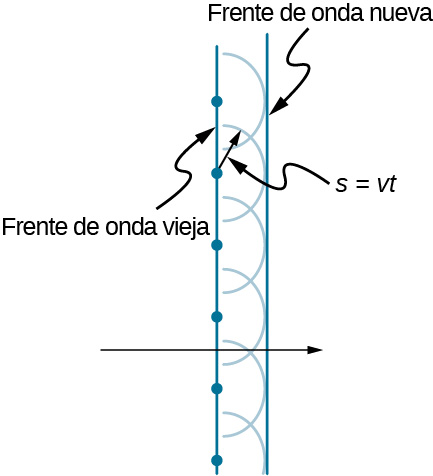
\includegraphics[width=\linewidth]{huygens_principle.jpg}
  \caption{Principio de Huygens}
  \label{fig:huygens_principle}
\end{wrapfigure}
Casi en paralelo, Christiaan Huygens (1678) propuso una teoría alternativa: la teoría ondulatoria de la luz. En lugar de partículas, la luz sería una perturbación en un medio elástico invisible ``el éter'' propagándose como ondas. Huygens explicó la refracción como resultado de velocidades distintas de propagación en diferentes medios y formuló el principio de Huygens, según el cual cada punto de un frente de onda es fuente de nuevas ondas secundarias.

Ambas teorías tenían fortalezas: Newton explicaba bien la geometría de los rayos y el fenómeno de la reflexión, mientras que Huygens ofrecía una mejor descripción de la difracción y la interferencia, fenómenos que aún no se habían explorado completamente.

Puedes leer más sobre este principio en OpenStax (\cite{openstax}: \href{https://openstax.org/books/f%C3%ADsica-universitaria-volumen-3/pages/1-6-principio-de-huygens}{Volumen 3, Principio de Huygens}).

\subsubsection{El renacimiento de la teoría ondulatoria}

A inicios del siglo XIX, los experimentos de Thomas Young (interferencia de doble rendija, 1801) y Augustin-Jean Fresnel (difracción) ofrecieron evidencia concluyente a favor de la teoría ondulatoria. Estos fenómenos no podían explicarse con partículas individuales, ya que mostraban patrones de superposición característicos de ondas. La luz se empezó a entender como una onda transversal, propagándose en el éter.

\subsubsection{Maxwell y el electromagnetismo}
\label{sec:maxwell_electromagnetismo}

Entre 1861 y 1865, James Clerk Maxwell formuló un sistema de ecuaciones que unificaba los fenómenos eléctricos y magnéticos: las ecuaciones de Maxwell. Al analizarlas, dedujo que las ondas electromagnéticas se propagaban en el vacío a una velocidad determinada por las constantes eléctricas y magnéticas del medio:

\[
v = \frac{1}{\sqrt{\mu_0 \varepsilon_0}} = \lambda f \approx 3 \times 10^8 \ \text{m/s}
\]

Esta velocidad coincidía exactamente con la de la luz. De este modo, la luz fue identificada como una onda electromagnética. Esto fue un triunfo de la teoría ondulatoria y de la física clásica. Sin embargo, las ecuaciones de Maxwell predecían \textbf{energía propagada} de forma continua, sin cuantización.

La figura \ref{fig:ond_electromagnetica} muestra una onda electromagnética. Vea que es una perturbación del campo eléctrico \(\vec{E}\) y del campo magnético \(\vec{B}\). Ambos son perpendiculares entre sí y también perpendiculares a la dirección de propagación de la onda.

\begin{figure}[ht]
  \centering
  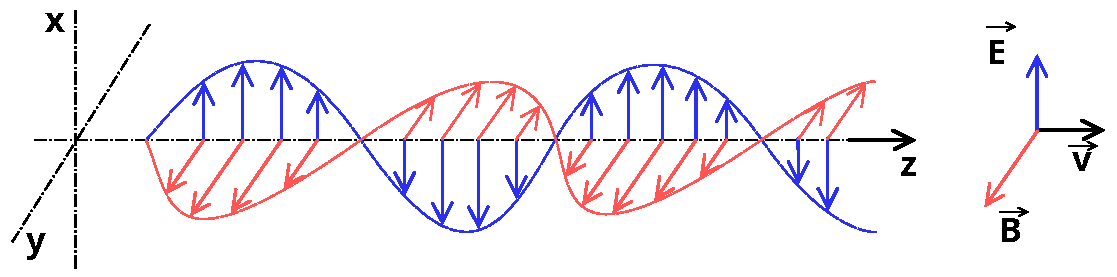
\includegraphics[width=0.8\textwidth]{electromagnetic_wave.pdf}
  \caption{Representación de una onda electromagnética.}
  \label{fig:ond_electromagnetica}
\end{figure}

El hecho de que las perturbaciones del campo eléctrico \(\vec{E}\) y del campo magnético \(\vec{B}\) en una onda electromagnética sean ortogonales (perpendiculares entre sí y a la dirección de propagación) no es un axioma ni una suposición: es una consecuencia directa de las ecuaciones de Maxwell en el vacío.

\paragraph{Demostración}

Consideremos una onda electromagnética plana que se propaga en el vacío en la dirección \(x\). Entonces buscamos soluciones de las ecuaciones de Maxwell donde los campos \(\vec{E}\) y \(\vec{B}\) dependen solo de \(x\) y del tiempo \(t\).

Queremos demostrar que:
\begin{itemize}
  \item \(\vec{E} \perp \vec{B}\)
  \item \(\vec{E} \perp \vec{k}\), donde \(\vec{k}\) es el vector de propagación (por ejemplo, en la dirección \(x\)).
\end{itemize}

Recordemos las ecuaciones de Maxwell en ausencia de cargas y corrientes (\(\rho = 0\), \(\vec{J} = 0\)):
\begin{align*}
  \nabla \cdot \vec{E} &= 0 \\
  \nabla \cdot \vec{B} &= 0 \\
  \nabla \times \vec{E} &= -\frac{\partial \vec{B}}{\partial t} \\
  \nabla \times \vec{B} &= \mu_0 \varepsilon_0 \frac{\partial \vec{E}}{\partial t}
\end{align*}

Vamos a usar estas ecuaciones para deducir la orientación relativa entre \(\vec{E}\), \(\vec{B}\), y la dirección de propagación.

Buscamos soluciones del tipo:

\[
\vec{E}(x,t), \quad \vec{B}(x,t)
\]

Asumamos que \(\vec{E}\) apunta en la dirección \(y\), y \(\vec{B}\) en la dirección \(z\):

\[
\vec{E} = E_y(x,t)\, \hat{y}, \quad \vec{B} = B_z(x,t)\, \hat{z}
\]

Dirección de propagación: \(\vec{k} = k\, \hat{x}\)

La tercera ecuación de Maxwell (ecuación de Faraday) nos dice que una variación en el campo magnético genera un campo eléctrico:
\[
\nabla \times \vec{E} = -\frac{\partial \vec{B}}{\partial t}
\]
El rotacional de \(\vec{E} = E_y(x,t)\, \hat{y}\) tiene solo una componente en \(z\):
\[
\nabla \times \vec{E} = \left( \frac{\partial E_y}{\partial x} \right) \hat{z}
\]
Entonces:
\[
\left( \nabla \times \vec{E} \right)_z = \frac{\partial E_y}{\partial x} = -\frac{\partial B_z}{\partial t}
\]

Este resultado indica que una variación del campo eléctrico \(E_y\) en la dirección de propagación \(x\) genera una variación temporal del campo magnético \(B_z\). Además, como las componentes están en direcciones ortogonales, se confirma que \(\vec{E} \perp \vec{B}\).

Análogamente, aplicamos la cuarta ecuación de Maxwell (ecuación de Maxwell-Ampère):
\[
\nabla \times \vec{B} = \mu_0 \varepsilon_0 \frac{\partial \vec{E}}{\partial t}
\]
Esta ecuación nos dice que una variación temporal del campo eléctrico genera un campo magnético.

El rotacional de \(\vec{B} = B_z(x,t)\, \hat{z}\) tiene componente en \(y\):
\[
\nabla \times \vec{B} = -\left( \frac{\partial B_z}{\partial x} \right) \hat{y}
\]
Entonces:
\[
\left( \nabla \times \vec{B} \right)_y = -\frac{\partial B_z}{\partial x} = \mu_0 \varepsilon_0 \frac{\partial E_y}{\partial t}
\]
Lo cual también es coherente con lo anterior.

\paragraph{Conclusión geométrica}

Los campos cumplen las siguientes condiciones:
\begin{itemize}
  \item \(\vec{E} \perp \vec{B}\), porque sus componentes son ortogonales \(y\) y \(z\),
  \item \(\vec{E} \perp \vec{k}\) y \(\vec{B} \perp \vec{k}\), porque ninguno depende de la componente \(x\) directamente.
\end{itemize}
Además, por el producto vectorial:
\[
\vec{E} \times \vec{B} \propto \vec{k}
\]
Es decir, la dirección de propagación es perpendicular a ambos campos, y se define por el producto vectorial de los campos.

Si la onda se propaga hacia la dirección \(x\):
\begin{itemize}
  \item \(\vec{E}\) oscila sobre el eje \(y\),
  \item \(\vec{B}\) oscila sobre el eje \(z\),
  \item La energía fluye en la dirección de \(\vec{E} \times \vec{B} = \hat{x}\).
\end{itemize}

\subsubsection{Crisis en la física clásica: la radiación del cuerpo negro}

A fines del siglo XIX, al estudiar la radiación del cuerpo negro, los físicos encontraron que la ley de Rayleigh-Jeans (derivada desde los supuestos clásicos) predecía una divergencia ultravioleta: una cantidad infinita de \textbf{energía}\footnote{Es importante que vea que el problema fue la \textbf{energía} que se emitía de forma continua, no el modelo ondulatorio. Ver la radiación electromagnética como onda es correcto, pero la energía que se emite de forma continua no lo es.} en las frecuencias altas, lo que claramente no ocurría en la realidad.

Para resolver esta contradicción, en 1900, Max Planck introdujo una hipótesis revolucionaria: la energía de la radiación electromagnética no se emite ni se absorbe de manera continua, sino en cuantos discretos, proporcionales a la frecuencia:

\begin{equation}
  E = h f
  \label{eq:planck}
\end{equation}
donde \(h=6.626 \times 10^{-34} \ \text{[Js]}\) es la constante de Planck. Este ajuste fue inicialmente visto como una herramienta matemática, no como una descripción física profunda.

\subsubsection{Einstein y el efecto fotoeléctrico: nacimiento del fotón}

En 1905, Albert Einstein retomó y radicalizó la idea de Planck para explicar el efecto fotoeléctrico que es el fenómeno por el cual un material emite electrones cuando es iluminado por luz. Este efecto fue observado experimentalmente desde finales del siglo XIX, pero no podía ser explicado mediante la teoría electromagnética clásica.

\begin{wrapfigure}{r}{0.3\textwidth}
  \centering
  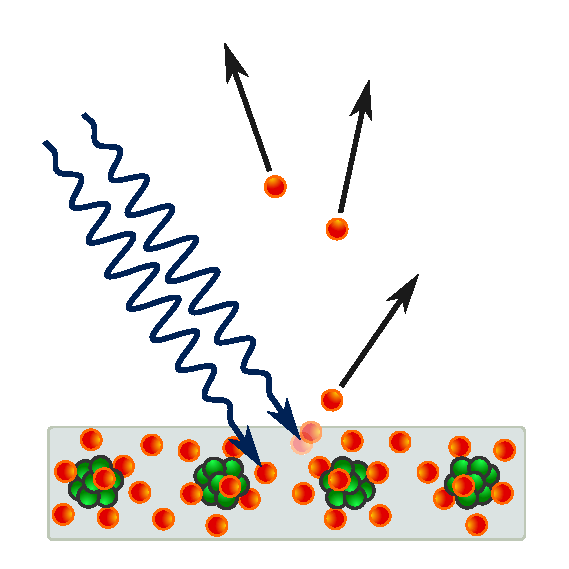
\includegraphics[width=\linewidth]{photoelectric_effect.pdf}
  \caption{Experimento típico: Se ilumina la superficie de un metal con luz de frecuencia conocida.}
  \label{fig:photoelectric_effect}
\end{wrapfigure}
Como se ve en la figura \ref{fig:photoelectric_effect} un experimento típico del efecto fotoeléctrico consiste en iluminar una placa metálica cargada eléctricamente con luz de una frecuencia conocida. Cuando se hace esto se observa que:
\begin{itemize}
  \item A frecuencias bajas, no se emiten electrones, sin importar cuán intensa sea la luz.
  \item A frecuencias suficientemente altas, sí se emiten electrones, incluso si la intensidad de la luz es débil.
  \item Si se aumenta la frecuencia de la luz por encima de cierto umbral, los electrones emitidos tienen mayor energía cinética.
\end{itemize}

Según la teoría clásica de ondas electromagnéticas, la energía asociada a las ondas como vimos en la sección \ref{sec:wave_energy} depende de la intensidad (\(I=P/S\)), entonces, la energía de la luz debería depender de la intensidad, no de la frecuencia. Es decir, una luz intensa debería poder arrancar electrones sin importar su frecuencia, dado suficiente tiempo.

Sin embargo, los experimentos mostraban lo contrario: una luz de baja frecuencia nunca arrancaba electrones, por más intensa que fuera. Esto no tenía explicación dentro del marco clásico.

Einstein propuso que la luz estaba compuesta de cuantos de energía localizados: fotones. Cada fotón tiene energía \(E = h f\), y al aplicar esta idea al efecto fotoeléctrico concluyó que un electrón dentro del metal solo puede absorber un fotón a la vez, y si ese fotón tiene suficiente energía, el electrón puede escapar del metal.

Para mayor elegancia formal se suele escribir usando la constante reducida \(\hbar = \frac{h}{2\pi}\), entonces:

\begin{equation*}
  E = \hbar \omega
\end{equation*}
donde \(\omega = 2\pi f\) es la frecuencia angular. Esta expresión es equivalente a la anterior.

\paragraph{La función de trabajo \(\phi\)}

Cada metal tiene una energía mínima necesaria para liberar un electrón de su superficie. Esta energía se llama función de trabajo y se denota con la letra griega \(\phi\):
\begin{equation*}
  \boxed{
    \phi = \text{energía mínima para extraer un electrón del metal}
  }
\end{equation*}

Entonces, si un fotón de energía \(E = h f\) incide sobre el metal:

\begin{itemize}
  \item Si \(h f < \phi\): no se emite ningún electrón (no importa la intensidad).
  \item Si \(h f \geq \phi\): el electrón es emitido y su energía cinética máxima es:
\end{itemize}

\begin{equation*}
  K_{\text{máx}} = \frac{1}{2} m_{e} v^2 = h f - \phi
\end{equation*}
donde \(m_e\) es la masa del electrón\footnote{Es muy importante que entienda que este efecto se cumple para los \textbf{electrones} (\(m_e = 9.11 \times 10^{-31} \ \text{kg}\)), no para protones, ya que se requiere muchísima más energía para arrancar un protón (\(m_p = 1.67 \times 10^{-27} \ \text{kg}\)).}. 

Este resultado coincide exactamente con los datos experimentales y contradice completamente las predicciones de la teoría clásica. Las implicaciones de esto son:

\begin{itemize}
  \item La energía de la luz está cuantizada.
  \item La intensidad de la luz afecta la cantidad de electrones emitidos, pero no su energía.
  \item Existe una frecuencia umbral \(f_0\) para cada metal, tal que si \(f < f_0\), no hay emisión fotoeléctrica.
\end{itemize}

Esta fue la primera evidencia directa de que la radiación electromagnética no solo tiene propiedades ondulatorias, sino también corpusculares.

Si quieres ver una prueba experimental del efecto fotoeléctrico, puedes ver el siguiente video: \href{https://youtu.be/oYnp0WZDhYQ?si=kIBH75DIIDv5hg_4}{YouTube: The Action Lab - The Photoelectric Effect}

\begin{tcolorbox}[myconclusion]
  En muchas ocasiones la energía se mide en electronvoltios (\(eV = \frac{1}{6.63 \times 10^{-34} \ \text{J}}\)), que es la energía necesaria para desplazar un electrón en un campo eléctrico de un voltio.
\end{tcolorbox}

\subsubsection{Conclusión: dualidad onda-partícula}

El desarrollo culminó en la aceptación de que la luz posee una naturaleza dual: se comporta como onda en fenómenos de interferencia y difracción, y como partícula en fenómenos como el efecto fotoeléctrico y el efecto Compton. Esta dualidad se extiende a la materia misma, como demostraría De Broglie en 1924, sentando las bases para la mecánica cuántica. Para la materia Física II solo usaremos la deducción final del efecto fotoeléctrico y la ecuación de energía de Planck.

\subsection{Espectro electromagnético}

El \textbf{espectro electromagnético} es la distribución de todas las formas posibles de radiación electromagnética, ordenadas según su frecuencia o longitud de onda. Comprende desde las ondas de radio, con longitudes de onda muy largas y baja frecuencia, hasta los rayos gamma, con longitudes de onda extremadamente cortas y alta frecuencia.

Toda radiación electromagnética es una forma de energía que se propaga en el espacio en forma de ondas que combinan campos eléctricos y magnéticos perpendiculares entre sí y a la dirección de propagación. Estas ondas no requieren de un medio material para propagarse.

El espectro electromagnético se divide, en términos generales, en las siguientes regiones:

\begin{figure}[ht]
  \centering
  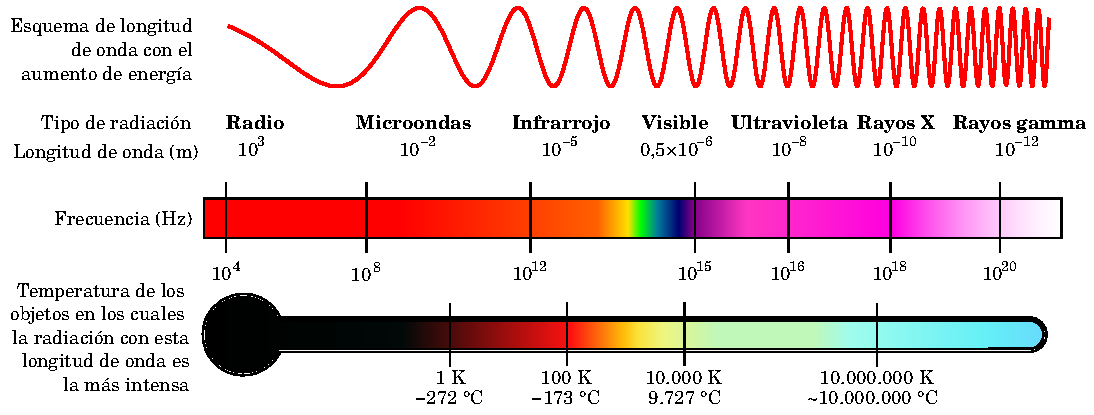
\includegraphics[width=1\textwidth]{em_spectrum.pdf}
  \caption{Espectro electromagnético}
  \label{fig:em_spectrum}
\end{figure}

Cada región del espectro tiene aplicaciones tecnológicas y científicas específicas. Por ejemplo, las ondas de radio se utilizan en telecomunicaciones, el infrarrojo en sensores térmicos, la luz visible en iluminación y visión, los rayos X en medicina, y los rayos gamma en tratamientos oncológicos.

En la figura \ref{fig:em_spectrum} se puede ver el espectro electromagnético ordenado según su longitud de onda. Vemos que a medida que la longitud de onda disminuye, la frecuencia aumenta. Esto es porque la longitud de onda y la frecuencia son inversamente proporcionales:
\[
  \lambda \propto \frac{1}{f}
\]
como vimos recién en la sección \ref{sec:maxwell_electromagnetismo} donde Maxwell demostró que la velocidad de la luz en el vacío es constante y es la misma para todas las regiones del espectro electromagnético. Por lo tanto, la longitud de onda y la frecuencia están relacionadas por la velocidad de la luz \(c\):
\[
  \lambda \cdot f = c = 299792458 \text{ m/s}
\]

\subsection{Fenómenos ondulatorios}

En la unidad anterior \ref{sec:waves_analisys} vimos de forma superficial algunos de los fenómenos ondulatorios. El único fenómeno que vimos con detalle fue la reflexión.

Ahora vamos a ver los fenómenos ondulatorios que aplican tanto a ondas mecánicas (como el sonido o las ondas en una cuerda) como a ondas electromagnéticas (como la luz o las microondas), con ciertas particularidades en cada caso.

En general los fenómenos ondulatorios son:

\begin{itemize}
  \item Reflexión
  \item Refracción
  \item Interferencia
  \item Difracción
  \item Polarización
\end{itemize}

\subsubsection{Reflexión}

\begin{wrapfigure}{r}{0.24\textwidth}
  \centering
  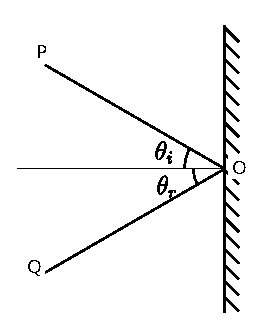
\includegraphics[width=\linewidth]{reflection_angles.pdf}
  \caption{Ángulos de reflexión}
  \label{fig:reflection_angles}
\end{wrapfigure}
La reflexión es el cambio en la dirección de propagación de una onda cuando choca contra una superficie y retorna al medio original.

Para ondas que inciden sobre una superficie lisa el ángulo de incidencia (\(\theta_i\)) es igual al ángulo de reflexión (\(\theta_r\)):
\[
  \theta_i = \theta_r
\]
Ejemplos:
\begin{itemize}
  \item Una onda en una cuerda que regresa al encontrar un extremo fijo.
  \item Un rayo de luz reflejándose en un espejo plano.
  \item Un eco producido por una onda sonora al rebotar en una pared.
\end{itemize}

\begin{wrapfigure}{l}{0.3\textwidth}
  \centering
  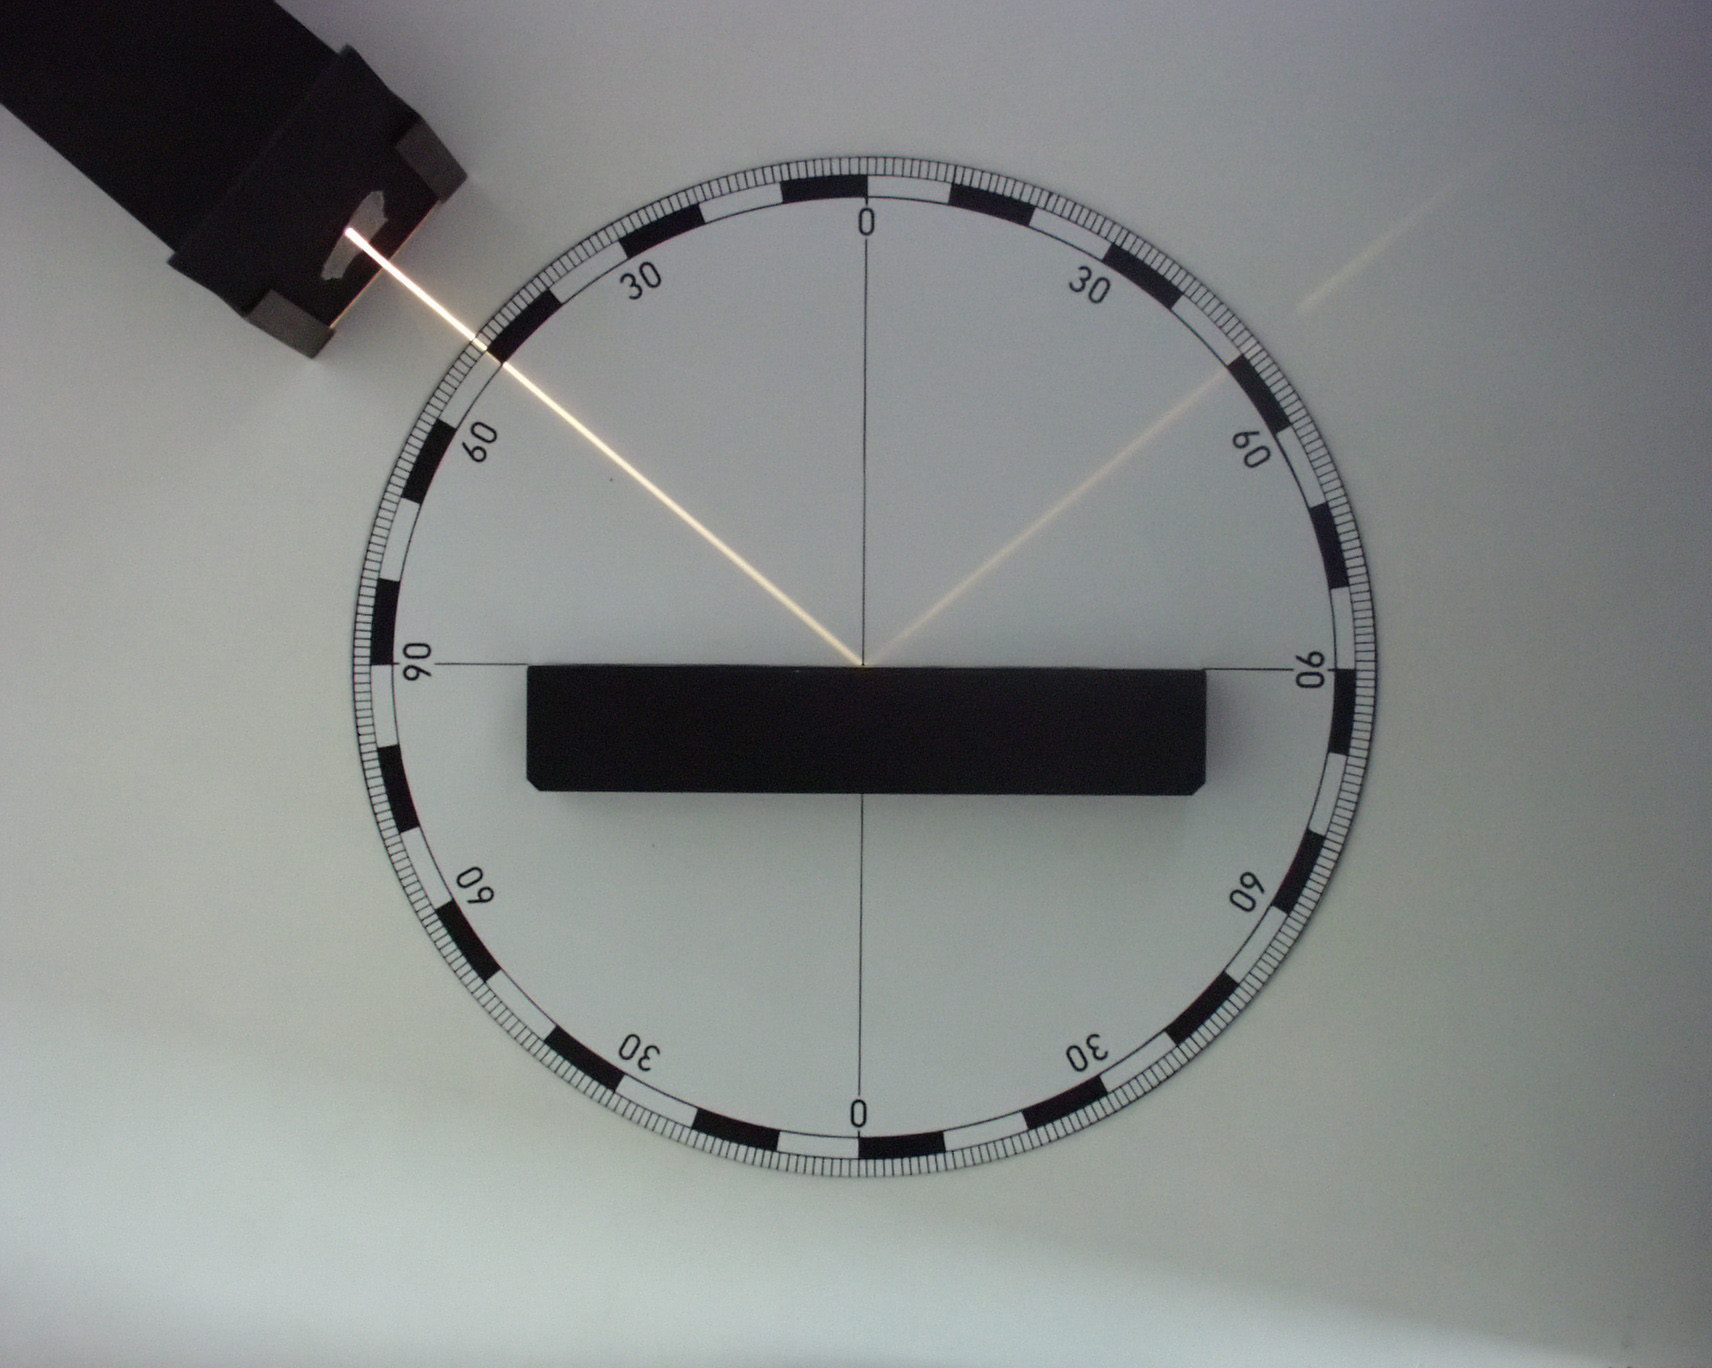
\includegraphics[width=\linewidth]{reflection_example.jpg}
  \caption{Reflexión de un haz de luz.}
  \label{fig:reflexion}
\end{wrapfigure}
En ondas mecánicas (como en cuerdas), la fase puede invertirse si la onda rebota en un medio más rígido (más denso). Se vió un ejemplo de esto con más detalle en la sección \ref{sec:waves_analisys}. 

En el caso de la luz (y en general cualquier onda electromagnética) también \textbf{puede invertir su fase} al reflejarse, dependiendo de las propiedades ópticas del medio en el que ocurre la reflexión.

La inversión de fase ocurre cuando una onda electromagnética se refleja en la superficie de \textbf{un medio con mayor índice de refracción que el medio del que proviene}. En ese caso, la onda reflejada experimenta un cambio de fase de \(\pi\) radianes (\(180^\circ\)).

En otras palabras, si la luz pasa de un medio con índice de refracción \(n_1\) a otro con \(n_2\), entonces:
\begin{itemize}
  \item Si \(n_2 > n_1\), la onda reflejada sufre un cambio de fase de \(\pi\) radianes (\(180^\circ\)).
  \item Si \(n_2 < n_1\), la onda reflejada no sufre un cambio de fase.
\end{itemize}

\subsubsection{Refracción y la ley de Snell}

La refracción es el fenómeno por el cual una onda electromagnética cambia de dirección y velocidad al pasar de un medio material a otro con diferente índice de refracción.

\begin{wrapfigure}{r}{0.3\textwidth}
  \centering
  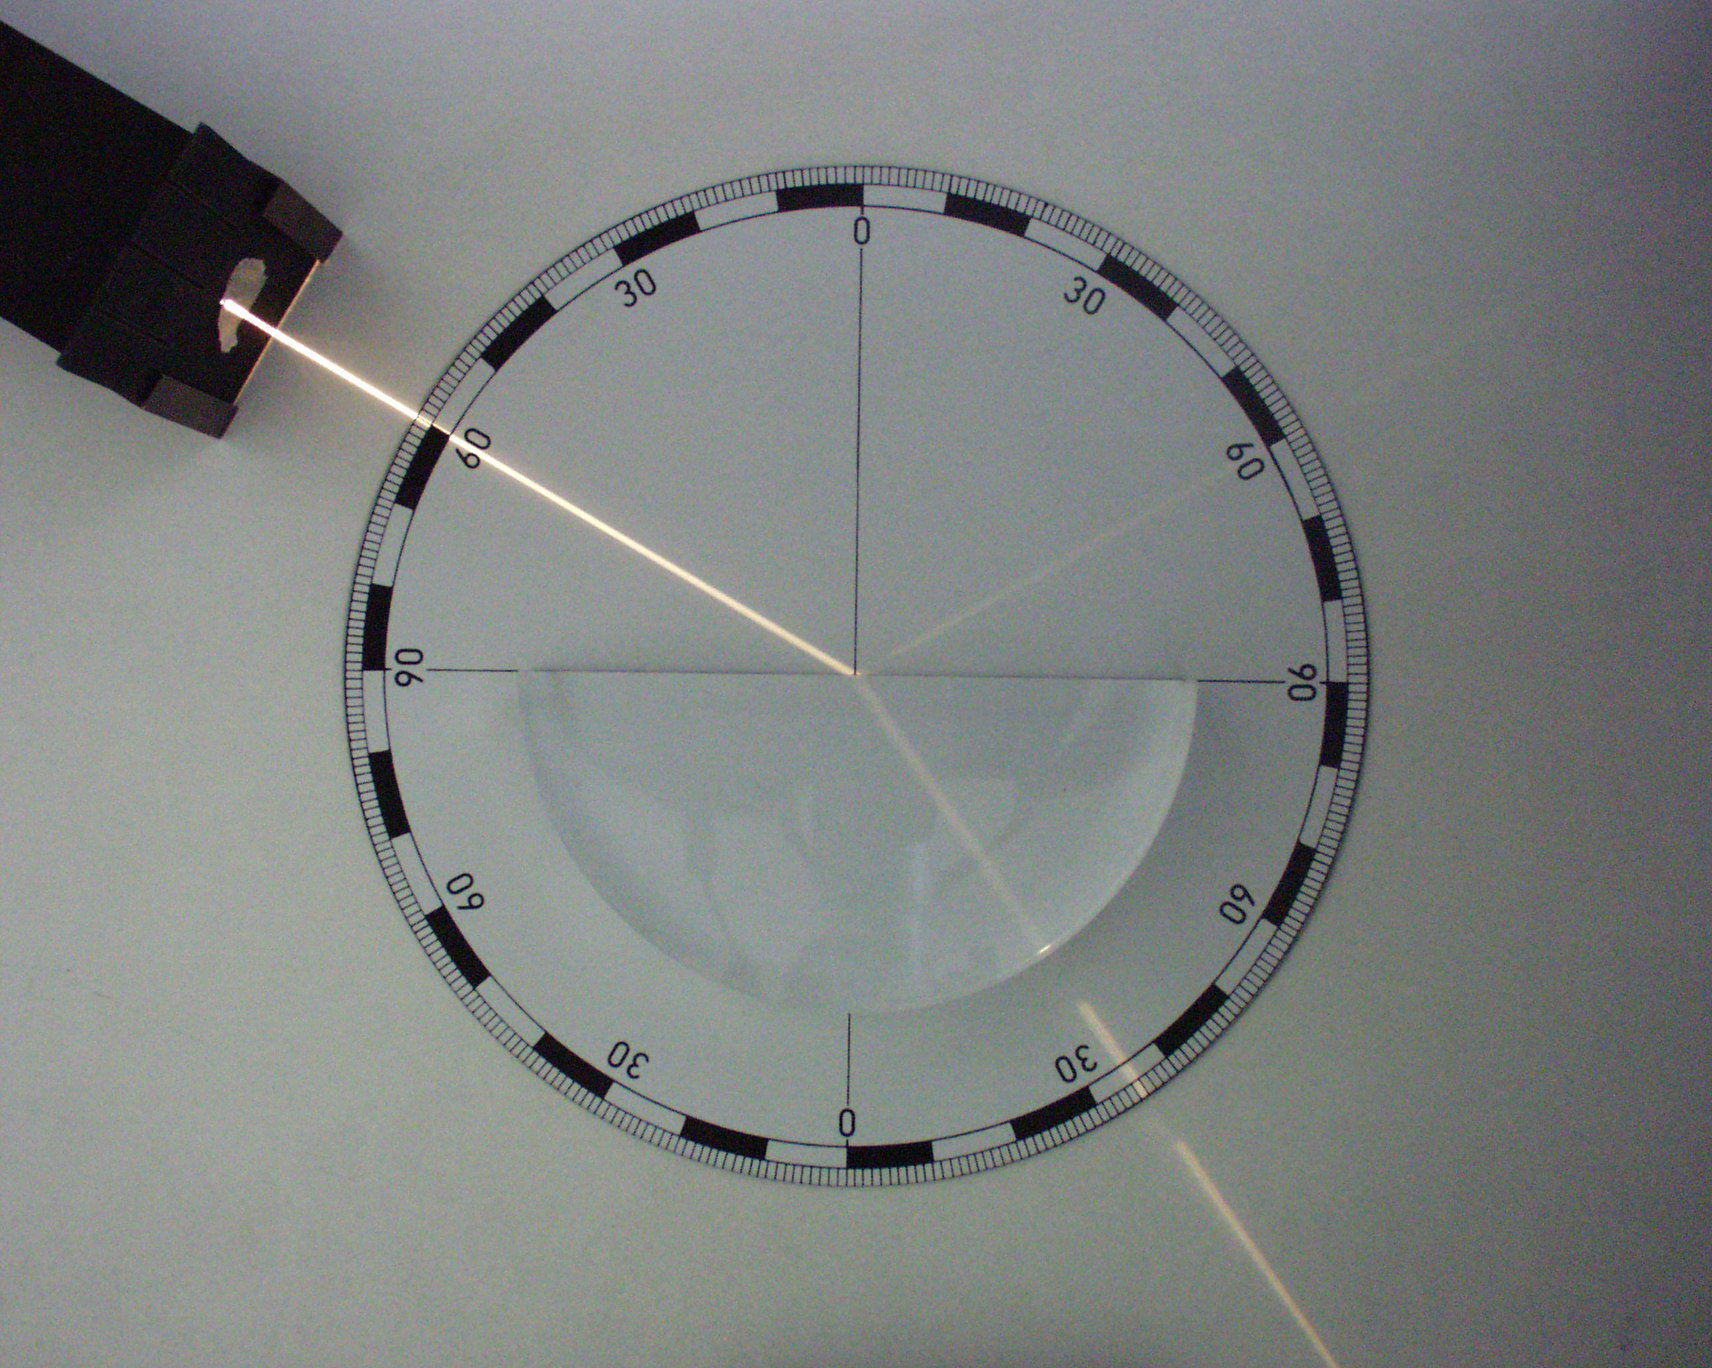
\includegraphics[width=\linewidth]{refraction_example.jpg}
  \caption{Refracción de un haz de luz.}
  \label{fig:refraction}
\end{wrapfigure}
Este cambio ocurre porque la velocidad de propagación de la onda no es la misma en distintos medios. Sin embargo, la frecuencia de la onda se conserva, lo cual implica que su longitud de onda cambia.

El índice de refracción \(n\) de un medio se define como:
\[
n = \frac{c}{v}
\]
donde:
\begin{itemize}
  \item \(c\) es la velocidad de la luz en el vacío.
  \item \(v\) es la velocidad de la onda en el medio.
\end{itemize}
Cuanto mayor es \(n\), más lento viaja la onda en ese medio.

\paragraph{Ley de Snell}

La dirección del rayo refractado está regida por la ley de Snell:
\[
n_1 \sin \theta_1 = n_2 \sin \theta_2
\]
donde:
\begin{itemize}
  \item \(n_1\), \(n_2\) son los índices de refracción de los medios 1 y 2.
  \item \(\theta_1\), \(\theta_2\) son los ángulos de incidencia y refracción medidos desde la normal a la superficie.
\end{itemize}

El límite o línea de separación entre los dos medios se llama frontera o interfaz.

\begin{figure}[ht]
  \centering
  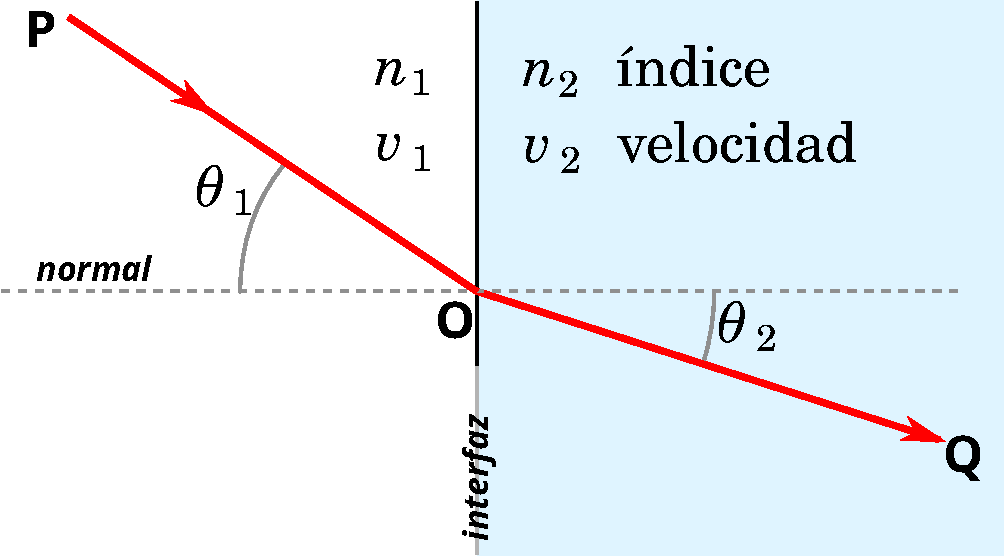
\includegraphics[width=0.5\textwidth]{snells_law.pdf}
  \caption{Ley de Snell.}
  \label{fig:snells_law}
\end{figure}

Cuando la onda cambia de medio la frecuencia \(f\) permanece constante (esto garantiza la continuidad temporal del campo eléctrico en la frontera), y la longitud de onda \(\lambda\) cambia según:
\[
\lambda_2 = \frac{v_2}{f} = \frac{c}{n_2 f}
\]
La dirección de propagación cambia si la onda incide oblicuamente.
\begin{itemize}
  \item Si \(n_2 > n_1\), la onda se desvía hacia la normal.
  \item Si \(n_2 < n_1\), se desvía lejos de la normal.
\end{itemize}
Sin embargo hay que tener en cuenta que existen casos especiales:
\begin{itemize}
  \item \textbf{Incidencia normal}: si la onda entra perpendicular a la superficie, no hay cambio de dirección, solo cambio en velocidad y longitud de onda.
  \item \textbf{Ángulo límite y reflexión total}: si la onda pasa de un medio más denso a uno menos denso y el ángulo de incidencia supera un cierto valor (ángulo crítico), no hay refracción, sino reflexión total interna.
\end{itemize}

\paragraph{Dispersion de la luz}

En términos simples, la \textbf{dispersión de la luz} es el fenómeno por el cual la luz blanca se separa en sus distintos colores (como los del arcoíris) cuando pasa a través de un material, como un prisma o gotas de agua.

Esto ocurre porque cada color de la luz viaja a una velocidad ligeramente diferente dentro del material, lo que provoca que se refracten en ángulos distintos. Los colores con menor longitud de onda, como el violeta o el azul, se desvían más que los de mayor longitud de onda, como el rojo.

\subsubsection{Interferencia}

La \textbf{interferencia} es un fenómeno característico de toda onda, y se refiere a la superposición de dos o más ondas coherentes que se encuentran en un mismo punto del espacio, generando un resultado que puede ser de mayor o menor intensidad, según la fase relativa entre ellas.

En el caso de ondas electromagnéticas, como la luz, la interferencia se manifiesta en variaciones de intensidad debidas a la superposición del campo eléctrico de las ondas.

Cuando dos ondas electromagnéticas se superponen, los campos eléctricos (\(\vec{E}\)) se suman vectorialmente (principio de superposición):
\[
\vec{E}_{\text{total}} = \vec{E}_1 + \vec{E}_2
\]
La intensidad observada es proporcional al cuadrado del campo eléctrico resultante:
\[
I \propto |\vec{E}_{\text{total}}|^2
\]
Esto puede generar dos situaciones:
\begin{enumerate}
  \item \textbf{Interferencia constructiva}: los campos eléctricos están en fase (máximos con máximos, mínimos con mínimos), y la intensidad aumenta.
  \item \textbf{Interferencia destructiva}: los campos están en oposición de fase (máximo con mínimo), y la intensidad disminuye o se anula.
\end{enumerate}

\paragraph{Condiciones necesarias para que haya interferencia observable}
\begin{itemize}
  \item Coherencia temporal: Las ondas deben tener frecuencias iguales o muy similares.
  \item Coherencia espacial: Las ondas deben mantener una diferencia de fase constante en el tiempo.
  \item Polarización compatible: Las componentes del campo eléctrico deben estar alineadas o parcialmente alineadas.
  \item Superposición espacial efectiva: Las ondas deben encontrarse en una región del espacio donde sus frentes de onda se crucen.
\end{itemize}

\paragraph{Diferencia de fase y camino óptico}

El camino óptico es una magnitud que permite cuantificar el efecto que tiene un medio sobre la propagación de una onda electromagnética, en particular sobre su fase. Se define como el producto del índice de refracción del medio y la distancia recorrida por la onda en ese medio.
\[
L = n \cdot d
\]
donde:
\begin{itemize}
  \item $L$ es el camino óptico,
  \item $n$ es el índice de refracción del medio,
  \item $d$ es la distancia física recorrida en el medio.
\end{itemize}
El camino óptico representa la distancia que la luz habría recorrido en el vacío durante el mismo tiempo que tarda en recorrer una distancia \(d\) en un medio con índice \(n\). Por eso, es útil para comparar fases entre ondas que han atravesado distintos medios. Dos ondas que recorren diferentes caminos ópticos pueden llegar con distinta fase al punto de interferencia, lo que afecta si la interferencia es constructiva o destructiva.

Cuando dos ondas recorren diferentes medios o longitudes, se habla de diferencia de camino óptico:
\[
\Delta L = n_1 d_1 - n_2 d_2
\]
Esta diferencia está directamente relacionada con la diferencia de fase:
\[
\Delta \varphi = \frac{2\pi}{\lambda_0} \Delta L
\]
donde \(\lambda_0\) es la longitud de onda en el vacío.

Entonces, retomando la ecuación de la interferencia, para que la interferencia sea observada, la diferencia de camino óptico \(\Delta L\) entre las ondas determina la diferencia de fase \(\Delta \varphi\) siendo:
\begin{itemize}
  \item Constructiva si \(\Delta L = m \lambda_0\), con \(m \in \mathbb{Z}\) (en fase (\(m\,2\pi\)))
  \item Destructiva si \(\Delta L = (m + 1/2)\lambda_0\) (en fase contraria (\(m\pi\)))
\end{itemize}
Algunos ejemplos típicos de interferencia son:
\begin{enumerate}
  \item Experimento de Young (doble rendija): produce franjas claras y oscuras por interferencia de la luz que pasa por dos rendijas muy cercanas.
  \item Interferencia en películas delgadas: como en burbujas de jabón o manchas de aceite, donde la luz se refleja en distintas capas.
\end{enumerate}

\begin{figure}[ht]
  \centering
  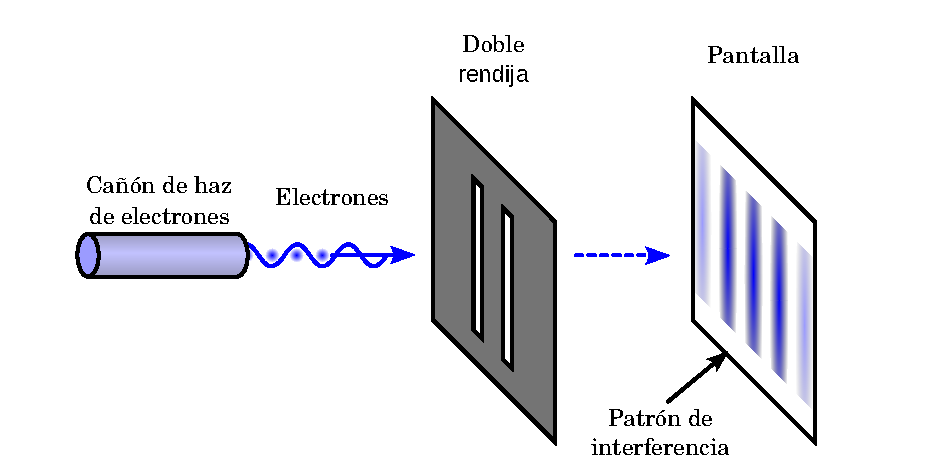
\includegraphics[width=0.65\textwidth]{double-slit.pdf}
  \caption{Interferencia de la luz por doble rendija}
  \label{fig:double_slit}
\end{figure}

\subsubsection{Difracción}

La difracción es la capacidad de una onda para rodear obstáculos o atravesar rendijas y luego extenderse en la región de sombra geométrica.

Factores relevantes:

\begin{itemize}
  \item Es más pronunciada si el tamaño de la rendija es comparable con la longitud de onda.
  \item A mayor longitud de onda, mayor difracción.
\end{itemize}

Ejemplos:

\begin{itemize}
  \item El sonido puede escucharse detrás de una pared aunque no haya línea de visión directa.
  \item Las ondas del mar rodean obstáculos como pilares o muelles.
\end{itemize}

\subsubsection{Polarización}

La polarización es la orientación de la vibración de una onda transversal en un solo plano. Solo ocurre con ondas transversales, como la luz; no ocurre con ondas longitudinales como el sonido.

Tipos de polarización:

\begin{itemize}
  \item Lineal: La onda vibra en un solo plano.
  \item Circular o elíptica: La dirección de vibración gira con el tiempo.
\end{itemize}

Métodos para polarizar la luz:

\begin{itemize}
  \item Filtros polarizadores (como en lentes de sol).
  \item Reflexión en ciertos ángulos (ángulo de Brewster).
  \item Dispersión (responsable del color azul del cielo).
\end{itemize}

Ejemplos:

\begin{itemize}
  \item Gafas de sol polarizadas que eliminan reflejos.
  \item Cristales líquidos en pantallas LCD utilizan luz polarizada.
\end{itemize}


\section{Electrostática}

La teoría electromagnética clásica estudia los fenómenos eléctricos y magnéticos, \hl{describiendo} sus características y las \hl{leyes} que los gobiernan.  

Cuando hablamos de \textbf{teoría clásica}, nos referimos a que se basa en la mecánica clásica de Isaac Newton. En esta mecánica se utilizan conceptos como partículas, trayectorias y las leyes del movimiento de Newton. De manera similar, en la teoría electromagnética se aplican estos conceptos a las cargas eléctricas y a los campos eléctricos y magnéticos. Es decir, en lugar de hablar solo de partículas y fuerzas mecánicas, hablaremos de \textbf{partículas cargadas, fuerzas eléctricas y campos electromagnéticos}.  

El electromagnetismo es una \hl{teoría de campos}. Por ejemplo, una \textbf{carga eléctrica} genera un \textbf{campo eléctrico} a su alrededor, mientras que un \textbf{imán} produce un \textbf{campo magnético} en el espacio que lo rodea. Estos campos son \hl{perturbaciones en el espacio} que afectan a otras cargas o imanes cercanos y pueden describirse matemáticamente.  

A lo largo de la historia, se ha comprobado que existen dos tipos de carga eléctrica: \textbf{positiva} y \textbf{negativa}. Las cargas del mismo tipo se repelen, mientras que las de signos opuestos se atraen.  

\subsection{Carga y Materia}

\subsection{Carga y Materia}

Todo lo que nos rodea, como una pelota, el aire, una planta o nuestro propio cuerpo, está formado por \textbf{átomos}. Los átomos, a su vez, están compuestos por tres tipos de partículas: \textbf{protones, neutrones y electrones}. Los protones y neutrones se encuentran en el núcleo del átomo, mientras que los electrones se mueven alrededor en la corteza. Los protones tienen \hl{carga positiva}, los electrones \hl{carga negativa}, y los neutrones no tienen carga. 

\begin{figure}[ht]
    \centering
    \includegraphics[width=0.4\textwidth]{atom_struct.jpg}
    \caption{Estructura básica de un átomo.}
    \label{fig:atom_struct}
\end{figure}

Esta estructura corresponde a un \textbf{modelo atómico}, que es una representación que nos ayuda a entender cómo está compuesto un átomo y cómo se comporta. A lo largo del tiempo han existido distintos modelos atómicos, pero uno de los más conocidos es el \textbf{modelo de Bohr}. Según este modelo, los electrones giran alrededor del núcleo en \textbf{órbitas circulares}, cada una con un nivel de energía específico. Cuando un electrón cambia de órbita, absorbe o emite energía en forma de luz.

La carga elemental \colorbox{highlight}{\( e \)} es la \textbf{cantidad más pequeña de carga eléctrica libre que se conoce en la naturaleza}. Es la carga que poseen los protones y electrones, pero con signo opuesto:
\begin{itemize}
    \item \textbf{Electrón}: \( -e = -1.602 \times 10^{-19} \) C (coulombs)
    \item \textbf{Protón}: \( +e = 1.602 \times 10^{-19} \) C
\end{itemize}

La carga elemental es fundamental porque todas las cargas eléctricas observadas en la naturaleza son \textbf{múltiplos enteros de \( e \)}. Es decir, cualquier carga presente en un objeto es el resultado de un exceso o déficit de electrones. Este principio se conoce como la \textbf{ley de conservación de la carga eléctrica}, y establece que la carga eléctrica \textbf{no se crea ni se destruye}, solo se transfiere de un cuerpo a otro.  

Los objetos tienen carga debido a la presencia de \textbf{electrones y protones}. Un objeto es eléctricamente neutro cuando tiene igual número de ambos. Si un objeto adquiere carga negativa, significa que ha \textbf{ganado electrones}, y si adquiere carga positiva, significa que ha \textbf{perdido electrones}. Cuando un objeto se carga, no se están creando nuevas cargas, sino que \textbf{se están moviendo electrones} de un cuerpo a otro. Por ejemplo: en la \textbf{electrización por frotamiento}, un material transfiere electrones a otro, dejando uno cargado positivamente y el otro negativamente. En la \textbf{inducción}, un objeto cargado puede redistribuir las cargas en otro sin tocarlo, pero sin cambiar la cantidad total de carga en el sistema.

En otras palabras, la carga eléctrica siempre se conserva porque \textbf{los electrones y protones no se destruyen en procesos normales}, solo cambian de ubicación dentro de un sistema.

\colorbox{highlight}{Denominaremos con la letra \( Q \) o \( q \) a la carga eléctrica de un objeto.} La carga se mide en \textbf{coulombs (C)}. Un coulomb es una cantidad de carga muy grande, por lo que en la práctica se utilizan submúltiplos como el \textbf{millicoulomb (mC)} o el \textbf{microcoulomb (\( \mu \text{C} \))}.

\subsubsection{Ley de Coulomb}

La electrostática estudia las cargas eléctricas en \hl{\textbf{reposo}}. La ley de Coulomb establece que \textbf{la fuerza entre dos cargas puntuales} es:

\begin{equation}
    F = k_e \frac{\abs{q_1} \cdot \abs{q_2}}{r^2}
    \label{eq:ley_coulomb}
\end{equation}

donde:

\begin{itemize}
    \item \( k_e \) es la constante de Coulomb: \( 8.9876 \times 10^9 \, \frac{\si{\newton\meter\squared}}{\si{\coulomb\squared}} \).
    \begin{itemize}
        \item \( k_e \) se obtiene de  \( \frac{1}{4\pi\epsilon_0} \) y,
        \item \( \epsilon_0 \) es la permitividad del vacío: \( 8.85 \times 10^{-12} \,\frac{\si{\coulomb\squared}}{\si{\newton\meter\squared}} \)
    \end{itemize}
    \item \( q_1 \) y \( q_2 \) son las cargas.
    \item \( r \) es la distancia entre las cargas.
\end{itemize}

Es muy importante notar que la \textbf{Ley de Coulomb} \eqref{eq:ley_coulomb} se aplica estrictamente a \hl{cargas puntuales}, es decir, cargas que se consideran concentradas en un solo punto sin dimensiones espaciales. En la ecuación anterior \eqref{eq:ley_coulomb}, se obtiene la magnitud de la fuerza eléctrica. La expresión vectorial de la fuerza eléctrica es:

\begin{equation}
    \vec{F}_e = k_e \frac{|q_1 q_2|}{r^2} \hat{r}
    \label{eq:ley_coulomb_vectorial}
\end{equation}

donde:
\begin{itemize}
    \item \( \vec{F}_e \) es el vector fuerza eléctrica entre dos cargas puntuales \( q_1 \) y \( q_2 \)
    \item \( \hat{r} \) es el vector unitario en la dirección que une ambas cargas.
\end{itemize}

Esto es importante tenerlo en cuenta ya que si se quiere saber la fuerza total sobre una carga \( q \) debido a varias cargas, se debe sumar vectorialmente las fuerzas individuales. La fuerza total sobre una carga \( q \) debido a un conjunto de cargas \( Q_i \) es:

\begin{equation}
    \vec{F} = \sum_i k \frac{|q \cdot Q_i|}{r_i^2} \hat{\mathbf{r_i}}
    \label{eq:ley_coulomb_vectorial_suma}
\end{equation}

\subsubsection{Cargas eléctricas}

La \textbf{carga eléctrica} es una propiedad fundamental de la materia que determina la interacción electromagnética entre partículas. Se trata de una magnitud escalar que puede ser de dos tipos: \textbf{positiva} o \textbf{negativa}. Las partículas con carga del mismo signo se repelen, mientras que las de signo opuesto se atraen.

La unidad de carga eléctrica en el \textbf{Sistema Internacional (SI)} es el \textbf{coulomb (\( \si{coulomb} \))}. La carga elemental está representada por la carga del electrón (\( -e = -1.602 \times 10^{-19} \si{coulomb} \)) y la del protón (\( e = +1.602 \times 10^{-19} \si{coulomb} \)).

\begin{center}
    \setlength{\arrayrulewidth}{1pt}  % Grosor de líneas
    \renewcommand{\arraystretch}{1.3} % Espaciado vertical
    \arrayrulecolor{gray} % Color de líneas

    \begin{tabular}{ c c c }
        \hline
        \rowcolor{asparagus!30}
        \textbf{Partícula}  & \textbf{Carga (\si{C})}           & \textbf{Masa (\si{kg})}   \\ \hline
        Electrón (e)        & \(-e = -1.602 \times 10^{-19}\)   & \(9.109 \times 10^{-31}\) \\
        Protón (p)          & \(+e = +1.602 \times 10^{-19}\)   & \(1.672 \times 10^{-27}\) \\
        Neutrón (n)         & \(0\)                             & \(1.675 \times 10^{-27}\) \\ \hline
    \end{tabular}
\end{center}

\subsubsection{Campo eléctrico}

Para entender la definición del campo eléctrico desde el principio, debemos pensar en cómo se conceptualiza la interacción entre cargas eléctricas y en la necesidad de definir una propiedad del espacio que describa esta interacción.

Sabemos que las cargas eléctricas ejercen fuerzas unas sobre otras. Experimentalmente, se observa que cargas del mismo signo se repelen y cargas de signo opuesto se atraen. Esta interacción fue formulada matemáticamente por la Ley de Coulomb \eqref{eq:ley_coulomb_vectorial}, sin embargo, esta ley solo nos dice cómo una carga afecta a otra en particular, \hl{pero no describe una propiedad del espacio en sí}. Aquí es donde se introduce el concepto de \textbf{campo eléctrico}.

\begin{figure}[ht]
    \centering
    \includegraphics[width=0.4\textwidth]{field_concept.png}
    \caption{Concepto de campo eléctrico.}
    \label{fig:concepto_campo_electrico}
\end{figure}

En lugar de pensar que una carga actúa instantáneamente sobre otra, se puede imaginar que una carga genera algo en el espacio a su alrededor que luego interactúa con otras cargas. Este ``algo'' es el \textbf{campo eléctrico}. La idea es la siguiente:

\begin{enumerate}
    \item Una carga fuente \( Q \) modifica el espacio circundante.
    \item Cualquier otra carga \( q \) que se coloque en ese espacio experimentará una fuerza debido a esta modificación.
    \item Para cuantificar esa modificación, definimos el campo eléctrico como la \textbf{fuerza por unidad de carga de prueba}.
\end{enumerate}

\paragraph{Idea conceptual del campo eléctrico}

Si te preguntas qué es el campo eléctrico, puedes responder según la descripción previa: ``el campo eléctrico es una propiedad del espacio que rodea a una carga eléctrica capaz de interactuar con otras cargas''. Sin embargo la idea es entender qué significa que una carga eléctrica modifique las propiedades del espacio que la rodea. Veamos un ejemplo de esto para entenderlo mejor.

Supongamos que tengo una carga positiva (un protón) y quiero que se quede totalmente quieto. Entonces ¿Cómo podemos lograr esto? 
Bueno, pues es bastante sencillo. Buscamos alguna carga \( Q \) que a una distancia \( r \) haga que la carga \( q \) del protón anule las fuerzas que interactúan con la carga.

Supongamos que la única fuerza que está interactuando con el protón es la fuerza peso. Entonces tendriamos que encontrar cualquier combinación de \( Q \) y \( r \) que cumpla:

\[
    F_g = F_e = k_e \frac{Q \cdot q}{r^2}
\]

Como nuestras incógnitas son \( Q \) y \( r \) vamos a tener infinitas posibilidades que solucionan muestro problema. Pero antes de dar por terminado el problema te pregunto ¿Qué tienen en común todas las soluciones?

Todas las soluciones están ocacionando el mismo efecto en el protón, una fuerza vertical y hacia arriba (en sentido opuesto al peso). Podriamos expresar esto diciendo: ``todas las soluciones generan una perturbación identica en el punto del espacio donde se encuentra el protón''. O, en otras palabras, todas las soluciones generan un campo eléctrico de las mismas características en donde está el protón.

Es más, cualquier partícula que coloquemos en el lugar del protón, con cualquier carga, por ejemplo una partícula con tres veces la carga del protón pero negativa, sentirá una fuerza proporcional a la que sentía el protón. En el caso de este ejemlo sería una fuerza igual a tres veces el peso del protón en el mimo sentido al peso (por ser negativa).

\paragraph{Formulando el Campo Eléctrico}

El campo eléctrico \( \vec{E} \) se define como la fuerza por unidad de carga de prueba \textbf{positiva} en un punto en el espacio. Esto puede expresarse como:

\begin{equation}
    \vec{E} = \frac{F}{q^{+}} = k_e \frac{Q}{r^2}
\end{equation}

donde:
\begin{itemize}
    \item \( Q \) es la carga que genera el campo (puntual).
    \item \( r \) es la distancia entre la carga de prueba y \( Q \).
\end{itemize}

En caso de que exista más de una carga que genera el campo, se aplica \textbf{el principio de superposición} que consiste en sumar todos todos los campos vectorialmente.

\[
\vec{E} = \sum{\vec{E}_i} = k \cdot \sum{\frac{Q_i}{r^2_i}} \hat{r}_i
\]

Sin embargo, en muchos casos, tenemos una distribución continua de carga en vez de una colección de cargas discretas. En esta situación, la carga puede estar distribuida a lo largo de una recta, sobre alguna superficie, por todo un volumen. Siguiendo el concepto de superposición de cargas tendríamos:

\[
\vec{E} = k \lim_{\Delta q_i \to 0} \sum_i{\frac{\Delta q_i}{r_i^2}\hat{r}_i} = k \int \frac{dq}{r^2} \hat{r}
\]

En los casos que debemos calcular el campo de una distribución continua tendremos la \textit{densidad de carga}. Pero ¿Qué es la densidad de carga?

La \textbf{densidad de carga} es una \textit{medida de cuánta carga eléctrica hay distribuida} sobre una determinada región del espacio. Se utiliza cuando las cargas no están concentradas en puntos, sino \textbf{distribuidas} sobre líneas, superficies o volúmenes.

Dependiendo del tipo de distribución, hay tres formas principales:

\subparagraph{1. Densidad lineal de carga:}

Se usa cuando la carga está distribuida a lo largo de una línea (como un alambre).

\[
\lambda = \frac{Q}{l} ~ ~ \rightarrow ~ ~ dq = \lambda dl
\]

\begin{itemize}
    \item \( \lambda \): densidad lineal (C/m)  
    \item \( Q \): pequeña cantidad de carga  
    \item \( l \): pequeña longitud del alambre  
\end{itemize}

\subparagraph{2. Densidad superficial de carga:}

Se usa para cargas sobre una superficie (como una lámina metálica cargada).

\[
\sigma = \frac{Q}{A} ~ ~ \rightarrow ~ ~ dq = \sigma dA
\]

\begin{itemize}
    \item \( \sigma \): densidad superficial (C/m²)  
    \item \( Q \): carga sobre un área pequeña  
    \item \( A \): área considerada  
\end{itemize}

\subparagraph{3. Densidad volumétrica de carga:}

Se usa cuando la carga ocupa un volumen (como una nube de plasma).

\[
\rho = \frac{Q}{V} ~ ~ \rightarrow ~ ~ dq = \rho dV
\]

\begin{itemize}
    \item \( \rho \): densidad volumétrica (C/m³)  
    \item \( Q \): carga dentro de un pequeño volumen  
    \item \( V \): volumen correspondiente  
\end{itemize}


Estas densidades permiten convertir una distribución continua de carga en una integral, y así calcular el campo eléctrico o el potencial.  
Por ejemplo, si conocés \( \lambda(x) \), podés calcular el campo eléctrico de una varilla cargada mediante:

\[
\vec{E} = \frac{1}{4\pi\varepsilon_0} \int \frac{\lambda(x)\, dx}{r^2} \hat{r}
\]

\paragraph{Visualización del campo eléctrico}

Para visualizar el campo eléctrico veamos un ejemplo sencillo. Supongamos que tenemos tres cargas eléctricas de distinto valor ubicadas en tres lugares distintos. Todas estas cargas están fijas en su posición y no pueden moverse (ver figura \ref{fig:campo_electrico_ejemplo_1}). 

\begin{figure}[ht]
    \centering
    \includegraphics[width=0.5\textwidth]{field_ex_1.png}
    \caption{tres cargas fijas en el espacio.}
    \label{fig:campo_electrico_ejemplo_1}
\end{figure}

Estas tres cargas posicionadas en el espacio constituyen lo que llamaremos \textbf{carga fuente}. Estas tres cargas fuente son capaces de generar una fuerza en cualquier partícula con carga que se coloque en este espacio. Podemos decir entonces, que las tres cargas le dan una propiedad eléctrica al espacio que las rodea. A esta propiedad que adquiere el espacio por culpa de las cargas le llamaremos campo eléctrico y existe independientemente de que haya otra cuarta carga presente o no.

Ahora supongamos que queremos jugar con el campo generado, y tomamos una cuarta carga \( q^{+} \), en este caso la carga será positiva, y la llamaremos \textbf{carga de prueba}. Entonces colocamos la carga de prueba en el centro de las tres cargas y la soltamos (ver figura \ref{fig:campo_electrico_ejemplo_2})

Cuando la soltamos, la carga será empujada hacia algún lugar, ya que, experimentará una fuerza debido a la interacción con las otras cargas. Ya sabemos que las cargas del mismo signo se repelen y las de signo opuesto se atraen.

\begin{figure}[ht]
    \centering
    \includegraphics[width=0.5\textwidth]{field_ex_2.png}
    \caption{colocamos una cuarta carga en el centro y la soltamos.}
    \label{fig:campo_electrico_ejemplo_2}
\end{figure}

Entonces aquí tenemos tres cargas aplicando tres fuerzas distintas, ¿qué hacemos? Sumar todas las fuerzas. Algunas se van a contrarrestar un poco al estar en direcciones opuestas, pero otras se van reforzar al tirar en el mismo sentido.

La suma de todas estas fuerzas (fuerza resultante) nos indica hacia dónde va ir la carga y la intensidad del empujón que sentirá (magnitud de la fuerza). Si realizamos esto en cada punto del espacio acabaríamos llenando el espacio de vectores de fuerza, esto se vería como un ``mapa de flechas'' que representan la fuerza que siente la carga de prueba en cada punto.

\textbf{Pero espera:} imaginemos que realizamos todos los cálculos con una carga de prueba de \( 1 \si{\coulomb} \). Y esa carga de prueba en realidad solo la usamos para realizar los cálculos del mapa, pero en realidad no existe. Entonces este mapa lo podemos usar para saber qué fuerza sentiría una carga \( q \) cualquiera.
Seguro te preguntarás ¿Cómo es eso? Es bien sencillo, presta atención a lo siguiente. Si recordamos la ecuación de la fuerza debido a la interacción entre cargas tenemos:

\[
\vec{F}_e = k\frac{Q\cdot q^{+}}{r^2}\hat{r} 
\]

Ahora, recordando que \( Q \) era nuestra carga fuente (formada por las tres cargas) y \( q^{+} \) nuestra carga de prueba de \( 1 \si{\coulomb} \) que usamos para hacer todas las cuentas, si quitamos la carga de prueba, como en la ecuación de fuerza es un factor neutro (multiplica por 1), el resultado no cambiaría cuantitativamente, sin embargo cambiarían las unidades. Veamos como queda:

\[
\vec{F}_e ~ [\si{\newton}] \neq k \frac{Q}{r^2} \hat{r} ~ [\si{\newton\per\coulomb}]
\]

Vemos que lo que resulta es una desigualdad, ya que las unidades no coinciden. Si bien numericamente es lo mismo, dimensionamente no. Para arreglar este problema entonces, en vez de quitar directamente la carga, podemos dividir ambos miembros por \( q^{+} \), y no romperíamos las unidades:

\[
\frac{\vec{F}_e}{q^{+}} ~ [\si{\newton\per\coulomb}] = k \frac{Q}{r^2} \hat{r} ~ [\si{\newton\per\coulomb}]
\]

\begin{figure}[ht]
    \centering
    \includegraphics[width=0.5\textwidth]{field_example.png}
    \caption{mapa de la fuerza que siente \(q^{+}\) en cada punto.}
    \label{fig:campo_electrico_ejemplo_3}
\end{figure}

¿Qué nos dice este ``mapa de flechas''? Este mapa de flechas nos dice la \hl{fuerza por unidad de carga} que generan las cargas fuente. Es decir, si colocamos una carga unidad (como \(q^{+}\)), entonces la relación es \(1:1\), pero podemos colocar cualquier carga \(q\) y multiplicarla por el campo.

\begin{equation}
    \vec{E} = \frac{\vec{F}}{q^{+}}
    \label{eq:campo_electrico}
\end{equation}

donde:
\begin{itemize}
    \item \( \vec{E} \) es el campo eléctrico en ese punto,
    \item \( \vec{F} \) es la fuerza experimentada por la carga de prueba \( q^{+} \),
    \item \( q^{+} \) es la carga de prueba.
\end{itemize}

Ahora, como vimos, la carga de prueba es una carga hipotética utilizada para medir el campo sin modificarlo. Como la carga de prueba es positiva, entonces vemos que una carga fuente \(Q\) cualquiera, respeta la siguiente distribución: si la carga \(Q\) es \textbf{negativa}, las líneas de campo son entrantes, si la carga \(Q\) es \textbf{positiva}, las líneas de campo son salientes:

\begin{figure}[ht]
    \centering
    \includegraphics[width=0.5\textwidth]{electric_field.jpg}
    \caption{Campo eléctrico de una carga puntual positiva y una negativa.}
    \label{fig:campo_electrico}
\end{figure}

Este resultado nos dice que el \hl{campo eléctrico} \textbf{se aleja} de cargas positivas y \textbf{se dirige hacia} cargas negativas. Además disminuye con el cuadrado de la distancia y es una propiedad del espacio ya no depende de la carga de prueba \( q \), sino solo de \( Q \).

Es muy importante tener en cuenta las premisas usadas para formular el \textbf{campo eléctrico}:
\begin{itemize}
    \item \textit{La carga fuente modifica el espacio circundante:} El campo eléctrico es una propiedad del espacio y es generado por una carga fuente.
    \item \textit{El campo es independiente de la carga de prueba:} La carga de prueba se usa solo como herramienta de medición.
    \item \textit{El campo es un campo vectorial:} Tiene dirección y magnitud en cada punto del espacio.
    \item \textit{El campo sigue el principio de superposición:} Si hay varias cargas, el campo total en un punto es la suma vectorial de los campos generados por cada una.
    \item \textit{La carga de prueba es positiva:} Para determinar el sentido del campo es importante tener en cuenta que la carga de prueba es positiva, esto permite ver con claridad cuando el campo es entrante o saliente para una carga puntual, o poder predecir correctamente el sentido del campo en una distribución de cargas (ya sea discreta o continua).
\end{itemize}

\subsubsection{Lineas de campo eléctrico}

Las líneas de campo no son más que un medio para visualizar el patrón formado por el campo eléctrico a través del trazo de líneas conocidas como \textbf{líneas de campo eléctrico}. Estas líneas relacionan el campo eléctrico con una región del espacio de la siguiente manera:
\begin{itemize}
    \item El vector \(\vec{E}\) del campo eléctrico es tangente a la línea del campo eléctrico en cada punto y la dirección de la linea de campo es igual a la del campo eléctrico.
    \item El número de líneas de campo que pasan por una superficie perpendicular a dichas líneas es proporcional a la magnitud de campo.
\end{itemize}

\begin{figure}[ht]
    \centering
    \includegraphics[width=0.5\textwidth]{field-lines.png}
    \caption{Líneas de campo eléctrico que atraviesan dos superficies}
    \label{fig:lineas_de_campo}
\end{figure}

Pongamos este concepto en palabras simples ¿Recuerdas el ejemplo de las tres cargas y el ``mapa de flechas''? Bueno, las líneas de campo nos ayudan a visualizar el ``mapa de flechas'' de una forma más cómoda.

\begin{figure}[ht]
    \centering
    \includegraphics[width=0.4\textwidth]{field_lines_ex.png}
    \caption{Ejemplo del ``mapa de flechas'' visualizado con líneas de campo}
    \label{fig:ej_lineas_de_campo}
\end{figure}

En este caso se puede ver que las líneas de campo están más juntas cuando nos acercamos a las cargas, y se van separando cuando nos alejamos. La proximidad entre líneas de campo nos indica que el campo es intenso. Si las líneas están distantes entre sí indica que el campo es menos intenso. Esto se puede verificar con la ecuación del campo eléctrico, ya que el campo disminuye con el cuadrado de la distancia. Esto significa que según más nos alejamos de las cargas fuente, el campo disminuye.

\subsection{Flujo eléctrico}

\subsection{Flujo eléctrico}
\label{sec:flujo_electrico}

Hasta ahora hemos visto una idea general de las líneas de campo eléctrico. Es decir, vimos una explicación que busca dar una idea general de cómo funcionan las líneas de campo eléctrico, su forma, su dirección y su relación con las cargas, pero sin proporcionar fórmulas o cantidades específicas. En este apartado, vamos a explicar con mayor formalidad este concepto, donde se considerará la magnitud del campo eléctrico y el área a través de la cual se mide el flujo eléctrico, utilizando la relación matemática entre estas variables.

\subsubsection{Definición}

El \hl{flujo eléctrico} es una medida de la cantidad de campo eléctrico que atraviesa una superficie dada. Se define matemáticamente como el producto de la magnitud del campo eléctrico (\(E\)) y el área (\(A\)) de la superficie a través de la cual se mide el flujo, así como el coseno del ángulo (\(\theta\)) entre la dirección del campo eléctrico y la normal (perpendicular) a la superficie. La fórmula para calcular el flujo eléctrico (\(\Phi_E\)) es:

\begin{figure}[ht]
    \centering
    \begin{subfigure}[b]{0.45\textwidth}
        \centering
        \includegraphics[width=\textwidth]{flujo_1.png}
        \caption{flujo sobre un area perpendicular.}
        \label{fig:flujo1}
    \end{subfigure}
    \hfill
    \begin{subfigure}[b]{0.45\textwidth}
        \centering
        \includegraphics[width=\textwidth]{flujo_2.png}
        \caption{flujo sobre un area inclinada.}
        \label{fig:flujo2}
    \end{subfigure}
    \caption{Flujo eléctrico}
    \label{fig:flujo eléctrico}
\end{figure}

\[
\Phi_E = E \cdot A \cdot \cos(\theta)  ~~ \left[\frac{\si{\newton \meter \squared}}{\si{\coulomb}}\right]
\]

Donde:
\begin{itemize}
    \item \(\Phi_E\) es el flujo eléctrico.
    \item \(E\) es la magnitud del campo eléctrico.
    \item \(A\) es el área de la superficie.
    \item \(\theta\) es el ángulo entre la dirección del campo eléctrico y la normal a la superficie.
\end{itemize}

Otra forma más general de escribir el flujo eléctrico es usando el \hl{producto escalar}. Para poder usar el producto escalar, necesitamos dos vectores, y en este caso solo tenemos el vector de campo. Entonce podemos definir un vector normal a la superficie con igual magnitud al área de la superficie. Entonces el producto escalar entre el vector campo eléctrico (\(\vec{E}\)) y el vector normal al area \(\vec{A}\) es:

\begin{equation}
    \Phi_E = \vec{E} \cdot \vec{A} = E A \cos \theta
    \label{eq:flujo_electrico}
\end{equation}

Hay que tener muy presente que \(\Phi_E\) es un \textbf{ESCALAR} no un vector. Y otro factor a considerar es que la ecuación \eqref{eq:flujo_electrico} solo se puede usar si el campo \(\vec{E}\) es constante. Sin embargo, en general, el campo \(\vec{E}\) no suele ser constante, entonces una forma de conseguir el flujo eléctrico total en una superficie \(S\) donde el campo no es constante es sumando todas las pequeñas contribuciones de flujo eléctrico en pequeñas porciones de area (\(dA\)), resultando en la siguiente integral:

\begin{equation}
    \Phi_E = \int_{S} \vec{E} \cdot d\vec{A}
    \label{eq:flujo_electrico_integral}
\end{equation}

\subsubsection{Ley de Gauss}
\label{sec:ley_de_gauss}

El flujo eléctrico es importante en el estudio del electromagnetismo porque está relacionado con la ley de Gauss, que establece que el flujo eléctrico a través de una superficie \textbf{cerrada} (con frecuencia llamada \textit{superficie gaussiana}) es proporcional a la carga eléctrica total encerrada dentro de esa superficie. Suponga una carga puntual positiva \(q\) ubicada en el centro de una esfera de radio \(r\) como se observa en la figura \ref{fig:superficie_gaussiana}.

\begin{wrapfigure}{r}{0.35\textwidth}
    \centering
    \includegraphics[width=\linewidth]{ley_de_gauss.png}
    \caption{Superficie gaussiana esférica de radio \(r\) que rodea una carga puntual \(q\).}
    \label{fig:superficie_gaussiana}
\end{wrapfigure}
De la ecuación de campo eléctrico \eqref{eq:campo_electrico}, se sabe que la magnitud del campo eléctrico sobre todos los puntos de la superficie (\(S\)) de la esfera es \(\vec{E} = k q/r^2\). Las líneas de campo están dirigidas radialmente hacia afuera y por tanto son perpendiculares a la superficie en todos sus puntos. Es decir, en cada punto de la superficie, \(\vec{E}\) es paralelo al vector \(d\vec{A}\) que representa un elemento de área muy pequeño que rodea al punto en la superficie. Por lo tanto, el flujo neto a través de la superficie gaussiana es igual a:

\begin{align*}
    \Phi_E =& \oint_S \vec{E} \cdot d\vec{A} \\
            =& \oint_S E \cos(0) ~ dA \\
            =& \oint_S E ~ dA \\
    \Phi_E =& E ~ \oint_S dA
\end{align*}
aquí tenemos que \(E=kq/r^2\) donde \(r\) es conocido y vale el radio de la esfera, \(q\) es el valor de la carga en el centro de la esfera y \(k = 1/4\pi\epsilon_0\). Luego la integral resulta en la superficie de una esfera que es \(4\pi r^2\). Entonces:

\[
\Phi_E = E ~ \oint_S dA = \frac{q}{4\pi \epsilon_0 r^2} \cdot 4\pi r^2 = \boxed{\frac{q}{\epsilon_0}} 
\]

Este resultado dice muchas cosas:
\begin{itemize}
    \item \textbf{Primero}: el flujo eléctrico \(\Phi_E\) no depende del radio de la superficie esférica.
    \item \textbf{Segundo}: el flujo es directamente proporcional a la carga encerrada en el interior de la superficie gaussiana.
    \item \textbf{Tercero}: el flujo es inversamente proporcional al valor de \(\epsilon\), en el ejemplo se trabajó con vacío, pero puede ser cualquier material no conductor con otro valor de \(\epsilon\).
\end{itemize}

En base a esto podemos sacar una conclusión, supongamos ahora que la superficie no es esférica ¿El flujo será el mismo que el de la esfera? Bueno, pues voy a hacer un adelanto, si lo es, pero ¿Por qué? Pensemos en la definición de flujo, sea cualquier superficie que rodea la esfera, el flujo será igual a el \(\vec{E}\cdot d\vec{A}\). Como vimos anteriormente esto representa la cantidad de líneas de campo que pasan por una superficie determinada. Como la superficie encierra la misma carga entonces saldrán la misma cantidad de líneas de campo por la superficie.

En este punto tal vez te preguntes ¿Cómo puede ser que no dependa del radio de la esfera, o mejor del tamaño de la superficie arbitraria cerrada? Es sencillo, si el tamaño de la superficie cerrada aumenta, entonces la distancia a la carga encerrada también aumentará, esto significa que la intensidad del campo disminuirá, entonces pasarán menos líneas de campo por cada \(dA\), pero como la superficie total a aumentado, entonces compensará la pérdida de intensidad del campo.

Con esto podemos armar una conclusión:

\begin{tcolorbox}[myconclusion]
    el flujo neto a través de \textit{cualquier} superficie cerrada que rodea a una carga puntual \(q\) está dado por \(q/\epsilon_0\) y es independiente de la forma de la superficie.
\end{tcolorbox}

Entonces, si suponemos varias superficies, llamemos \(S1\), \(S2\) y \(S3\) a las superficies que rodean la carga \(q\) (ver figura \ref{fig:superficie_gaussiana_arbitraria}). Todas estas superficies tienen el mismo flujo eléctrico, ya que todas encierran la misma carga \(q\). Se puede ver que el flujo neto es el mismo para todas las superficies.

\begin{figure}[ht]
    \centering
    \includegraphics[width=0.35\textwidth]{flujo_neto.png}
    \caption{Distintas superficies gaussianas de forma arbitraria que rodean una carga puntual \(q\).}
    \label{fig:superficie_gaussiana_arbitraria}
\end{figure}

Por otro lado, si la carga \(q\) está fuera de la superficie gaussiana entonces la misma cantidad de líneas de campo que entran por un lado de la superficie, salen por el otro lado. Por lo tanto, el flujo neto a través de la superficie es cero. Esto se puede ver en la figura \ref{fig:flujo_neto_2} donde se observa que el flujo neto es cero.

\begin{figure}[ht]
    \centering
    \includegraphics[width=0.4\textwidth]{flujo_neto_externo.png}
    \caption{Una carga puntual \(q\) fuera de la superficie.}
    \label{fig:flujo_neto_2}
\end{figure}

La forma matemática de ley de Gauss, es una generalización de lo anterior y establece que el flujo neto a través de cualquier superficie cerrada es

\begin{equation}
    \Phi_E = \oint_{S} \vec{E} \cdot d\vec{A} = \frac{q_{\text{int}}}{\varepsilon_0} ~~ \left[\frac{\si{\newton \meter \squared}}{\si{\coulomb}}\right]
\end{equation}
donde:
\begin{itemize}
    \item \( \Phi_E \) es el flujo de campo eléctrico a través de una superficie cerrada.
    \item \(E\) es el campo eléctrico en cada punto de esa superficie.
    \item \(dA\) es un vector diferencial de área que apunta hacia afuera de la superficie.
    \item \(q_{int}\) es la carga total encerrada dentro de la superficie.
    \item \(\epsilon_0\) es la permitividad del vacío, una constante del medio.
\end{itemize}

\begin{tcolorbox}[mydanger]
    CUIDADO: \(\vec{E}\) representa el campo eléctrico total, que incluye contribuciones de ambas cargas tanto del interior como del exterior de la superficie.    
\end{tcolorbox}

\paragraph{¿Qué nos dice esta ley, en términos simples?}

El flujo eléctrico representa la cantidad de ``líneas de campo eléctrico'' que atraviesan una superficie. La ley de Gauss nos habla de superficies cerradas, y nos dice que si hay carga dentro de una superficie cerrada, el campo eléctrico ``sale'' (o ``entra'') por esa superficie, generando un flujo distinto de cero. Si no hay carga neta dentro, el flujo eléctrico total es cero, aunque el campo pueda no ser nulo en todos los puntos. No importa la forma de la superficie, solo importa cuánta carga encierra, no cómo se distribuye el campo en detalle.

\subparagraph{¿Por qué es útil la ley de Gauss?}

La ley de Gauss es útil porque, en situaciones con alta simetría (esférica, cilíndrica, planar), permite calcular el campo eléctrico sin integrar la ley de Coulomb, por ejemplo:
\begin{itemize}
    \item Una esfera cargada uniformemente
    \item Un hilo infinitamente largo con carga lineal uniforme
    \item Un plano infinito cargado
\end{itemize}

\subparagraph{Ejemplo clásico: esfera cargada}

Supón una carga distribuida uniformemente en una esfera. Si elegimos una superficie esférica de radio  mayor al de la esfera, por simetría:
\[
\vec{E} = \text{constante} \quad \text{y} \quad \vec{E} \parallel d\vec{A}
\]
Entonces la integral se simplifica:
\[
\oint \vec{E} \cdot d\vec{A} = E \oint dA = E(4\pi r^2)
\]
Y por la ley de Gauss:
\[
E(4\pi r^2) = \frac{Q}{\varepsilon_0} \quad \Rightarrow \quad E = \frac{1}{4\pi\varepsilon_0} \frac{Q}{r^2}
\]
¡Y así recuperamos la fórmula del campo eléctrico de una carga puntual!

\subsection{Potencial eléctrico}

\subsection{Potencial eléctrico}

Cuando se coloca una carga \(q\) en un campo eléctrico \(\vec{E}\), la carga experimenta una fuerza \(\vec{F}=q\vec{E}\). Esta fuerza es conservativa, lo que significa que el trabajo realizado por la fuerza al mover la carga entre dos puntos \(A\) y \(B\) no depende de la trayectoria seguida, sino solo de los puntos inicial y final.

El trabajo realizado por la fuerza al mover la carga \(q\) desde el punto \(A\) hasta el punto \(B\) se define como:
\begin{equation*}
    W_{AB} = \int_A^B \vec{F} \cdot d\vec{s} = \int_A^B q\vec{E} \cdot d\vec{s}
\end{equation*}
donde \(d\vec{s}\) es un elemento diferencial de desplazamiento a lo largo de la trayectoria. Y como la fuerza eléctrica es conservativa, podemos expresarla en términos de la energía potencial eléctrica \(U\):
\begin{equation*}
    W_{AB} = U_A - U_B = -\Delta U
\end{equation*}

\subsubsection{Definición de potencial eléctrico}

Para una posición conocida de la carga de prueba en el campo, el sistema carga-campo tiene una energía potencial \(U\) relativa a la configuración del sistema definida como \(U=0\). Al dividir la energía potencial entre la carga de prueba \(q\), obtenemos el \textbf{potencial eléctrico} \(V\) en un punto \(P\) del campo eléctrico:

\begin{equation}
    V = \frac{U}{q}
    \label{eq:potential}
\end{equation}

El potencial eléctrico es una magnitud escalar que se mide en \(\text{V}\) (voltios) y se define como la energía potencial por unidad de carga.

Teniendo en cuenta la definición de potencial (ecuación \eqref{eq:potential}) la \textbf{diferencia de potencial} \(\Delta V = V_B - V_A\) entre dos puntos \(A\) y \(B\) en un campo eléctrico se define como el cambio en energía potencial por unidad de carga al mover una carga de prueba \(q\) entre esos dos puntos:

\begin{equation}
    \Delta V = \frac{\Delta U}{q} = -\int_A^B \vec{E} \cdot d\vec{s}
    \label{eq:potential_difference}
\end{equation}

Por la ecuación \eqref{eq:potential_difference}, el trabajo realizado por un agente externo al desplazar una carga \(q\) a través de un campo eléctrico con una velocidad constante es:

\[
W=q\Delta V
\]

Es muy importante que el desplazamiento de la carga \(q\) sea a velocidad constante, ya que si no lo es, el trabajo realizado por el agente externo no será igual al trabajo realizado por la fuerza eléctrica. 

Nótese que el concepto de potencial eléctrico se concive de forma similar al de campo eléctrico. Se usa una carga de prueba positiva \(q\) haciendo que sólo dependa de la carga fuente \(Q\) que genera el campo eléctrico. 

\subsubsection{Diferencia de potencial en un campo eléctrico uniforme}

La ecuación \eqref{eq:potential_difference} es válida en todos los campos eléctricos, sean uniformes o no. En un campo eléctrico uniforme, la magnitud del campo \(\vec{E}\) es constante y la dirección de \(\vec{E}\) es la misma en todos los puntos del campo. En este caso, la diferencia de potencial entre dos puntos \(A\) y \(B\) separados por una distancia \(d\) en la dirección del campo eléctrico se puede expresar como:
\begin{equation}
    \Delta V = -\int_A^B \vec{E} \cdot d\vec{s} = -E \, \int_A^B ds = \boxed{-Ed}
    \label{eq:potential_uniform}
\end{equation}
donde \(E\) es la magnitud del campo eléctrico y \(d\) es la distancia entre los puntos \(A\) y \(B\) en la dirección del campo.

El signo negativo indica que el potencial en el punto \(B\) es menor que el potencial en el punto \(A\) si la carga de prueba se mueve en la dirección del campo eléctrico. Esto significa que el trabajo realizado por la fuerza eléctrica es negativo, lo que implica que la energía potencial disminuye al mover la carga en la dirección del campo eléctrico.

\begin{figure}[ht]
    \centering
    \includegraphics[width=1\textwidth]{potential_const_field.png}
    \caption{Comparación de la energía potencial eléctrica y gravitatoria.}
    \label{fig:potential_uniform}
\end{figure}

\begin{tcolorbox}[mydanger]
    CUIDADO: si la carga \(q\) es negativa, la situación se invierte. El sistema gana energía potencial al mover la carga \(q\) en la dirección del campo eléctrico, y disminuye al moverla en la dirección opuesta.    
\end{tcolorbox}

\subsubsection{Potencial eléctrico debido a una carga puntual}

\begin{wrapfigure}{l}{0.32\textwidth}
    \centering
    \includegraphics[width=\linewidth]{puntual_potential_1.png}
    \caption{Potencial en el punto \(P\) debido a \(q_1\).}
    \label{fig:potential_point_charge}
\end{wrapfigure}

Como se menciona en la definición, la energía potencial es relativa al punto que se ha definido como ``0''. Con  el potencial eléctrico pasa lo mismo, entonces si queremos saber el potencial en un punto \(P\) del campo eléctrico, sabemos que es igual al trabajo realizado por la fuerza eléctrica al mover una carga de prueba \(q\), pero ¿Desde donde hasta donde? Bueno, podemos definir que nuestro potencial sea cero cuando la carga \(q\) esté infinitamente alejada de la fuente. Entonces el potencial en el punto \(P\) es trabajo para mover la carga de prueba desde el infinito hasta el punto \(P\):

\begin{align*}
    V_P &= - \lim_{a \to \infty}\int_{a}^P \vec{E} \cdot d\vec{r}\\
        &= - \lim_{a \to \infty}\int_{a}^P \frac{kq_1}{r^2} \cdot dr\\
        &= -kq_1 \, \lim_{a \to \infty} \int_{a}^P \frac{1}{r^2} \cdot dr\\
        &= -kq_1 \, \lim_{a \to \infty} \left[ -\frac{1}{r} \right]_{a}^P\\
        &= -kq_1 \, \lim_{a \to \infty} \left[ -\frac{1}{P} + \frac{1}{a} \right]\\
        &= -kq_1 \, \left[ -\frac{1}{P} + 0 \right] \\
    V_P &= k\frac{q_1}{r_{12}} = \lVert\vec{E}\rVert \, \lVert\vec{r}_{12}\rVert \cos(0)
\end{align*}
por ser \(\vec{E}\) y \(\vec{r}_{12}\) paralelos. Entonces el potencial eléctrico en un punto \(P\) debido a una carga puntual \(q_1\) es:
\begin{equation}
    \boxed{V_P = k\frac{q_1}{r_{12}} = E \, r_{12}}
    \label{eq:potential_point_charge}
\end{equation}
donde \(q_1\) es la carga fuente, \(E\) el campo generado por \(q_1\) y \(r_{12}\) la distancia a un punto en el campo eléctrico.

El potencial eléctrico debido a múltiples cargas puntuales se basa en el principio de superposición, que establece que el potencial eléctrico total en un punto es igual a la suma algebraica de los potenciales individuales producidos por cada carga.

\begin{equation}
    V_{total} = \sum_{i=1}^{n} V_i = k \sum_{i=1}^{n} \frac{q_i}{r_i}
\end{equation}

\subsubsection{Obtención de \texorpdfstring{\(\vec{E}\)}{E} a partir de \texorpdfstring{\(V\)}{V}}

El campo eléctrico \(\vec{E}\) y el potencial eléctrico \(V\) están relacionados, como se muestra en la ecuación \eqref{eq:potential_point_charge}, que se usa para encontrar \(V\) en un punto cuando se conoce \(\vec{E}\). Sin embargo, también podemos encontrar \(\vec{E}\) a partir de \(V\) usando la relación:

\begin{equation}
    dV = -\vec{E} \cdot d\vec{s}
    \label{eq:field_from_potential_differential}
\end{equation}
y si estamos trabajando con una única coordenada podemos escribir la ecuación \eqref{eq:field_from_potential_differential} como:

\[
    dV = -E \, ds \quad \Rightarrow \quad E = -\frac{dV}{ds}
\]

Sin embargo, en general, el potencial eléctrico es una función de las tres coordenadas espaciales. Si \(V(r)\) se da en coordenadas cartesianas, las componentes \((E_x, E_y, E_z)\) del campo eléctrico pueden ser determinadas fácilmente a partir de \(V(x, y, z)\) como derivadas parciales

\begin{equation}
    \vec{E} = -\nabla V
    \label{eq:field_from_potential}
\end{equation}
donde \(\nabla\) es el operador nabla, que representa el \hl{gradiente del potencial eléctrico}. Esta relación indica que el campo eléctrico es igual al negativo del gradiente del potencial eléctrico. En otras palabras, el campo eléctrico apunta en la dirección de mayor disminución del potencial eléctrico.

\paragraph{Recordatorio: operador nabla}

El operador \textbf{nabla} (\(\nabla\)), también conocido como \textbf{operador del gradiente}, es una herramienta matemática usada en cálculo vectorial y análisis multivariable. Se utiliza para representar derivadas en múltiples dimensiones.

Formalmente, el operador nabla se define como:

\[
\nabla = \left( \frac{\partial}{\partial x}, \frac{\partial}{\partial y}, \frac{\partial}{\partial z} \right)
\]

Es un operador vectorial que, aplicado a diferentes tipos de funciones, da lugar a distintos conceptos. En nuestro caso solo vamos a repasar el concepto de gradiente.

Cuando se aplica el operador nabla a una función escalar \( f(x, y, z) \), produce un \textbf{campo vectorial} que apunta en la dirección de mayor incremento de la función. Se expresa como:

\[
\nabla f = \left( \frac{\partial f}{\partial x}, \frac{\partial f}{\partial y}, \frac{\partial f}{\partial z} \right)
\]

Este vector resultante indica la dirección en la que la función crece más rápidamente y su magnitud corresponde a la tasa de cambio máxima. En el caso de \(\vec{E}\) y \(V\), \(\vec{E}\) es el gradiente de \(V\) representa una función vectorial que apunta en la dirección de mayor aumento del potencial eléctrico.

\subsection{Capacitores}

Un \textbf{capacitor}, también conocido como \textbf{condensador}, es un componente eléctrico pasivo que tiene la capacidad de \textbf{almacenar energía en forma de un campo eléctrico}. Está compuesto por dos conductores (llamados placas) separados por un material dieléctrico, que actúa como aislante.

Cuando se aplica una diferencia de potencial (voltaje) entre las placas, una de ellas acumula carga positiva y la otra carga negativa, generando así un campo eléctrico entre ellas. La capacidad del capacitor para almacenar carga depende de sus características físicas y del dieléctrico utilizado.

La \textbf{capacitancia} es una medida de esa capacidad de almacenamiento de carga eléctrica. Se define como:

\begin{equation}
    C = \frac{Q}{V}
    \label{eq:capacitance}    
\end{equation}

donde:

\begin{itemize}
    \item \( C \) es la \textbf{capacitancia} del capacitor, medida en faradios (\(\si{\farad}\)).
    \item \( Q \) es la \textbf{carga eléctrica} almacenada en el capacitor, medida en coulombs (\(\si{\coulomb}\)).
    \item \( V \) es la \textbf{diferencia de potencial} entre las placas del capacitor, medida en voltios (\(\si{\volt}\)).
\end{itemize}

Un faradio es una unidad muy grande, por lo que en la práctica suelen utilizarse submúltiplos como el microfaradio (\(\mu\si{farad}\)), nanofaradio (n\(\si{\farad}\)) o picofaradio (p\(\si{\farad}\)).

La capacitancia depende de factores. Si se tienen placas paralelas de depende de factores como el área de las placas (\(A\)), la distancia entre ellas (\(d\)) y la permitividad del dieléctrico (\( \varepsilon \)) según la siguiente fórmula:

\[
C = \varepsilon \frac{A}{d}
\]

Este comportamiento hace que los capacitores sean ampliamente utilizados en circuitos electrónicos para funciones como almacenamiento de energía, filtrado, acoplamiento y desacoplamiento de señales, entre otras.

\subsubsection{Geometría de los conductores}

Cuando la \hl{geometría de los conductores} es distinta a la de un capacitor de placas planas y paralelas, la expresión de la capacitancia cambia, aunque el principio físico fundamental sigue siendo el mismo: almacenar energía en forma de campo eléctrico entre conductores separados por un dieléctrico.

En general, la \hl{capacitancia depende de la geometría de los conductores y del medio dieléctrico entre ellos}. A continuación, se presentan algunos casos comunes:

\paragraph{1. Capacitor esférico}

Consiste en dos esferas concéntricas de radios \( R_1 \) (interna) y \( R_2 \) (externa). Su capacitancia es:

\[
C = 4\pi \varepsilon_0 \varepsilon_r \frac{R_1 R_2}{R_2 - R_1}
\]

\paragraph{2. Capacitor cilíndrico}

Está formado por dos cilindros coaxiales, uno de radio interno \( a \) y otro de radio externo \( b \), y de longitud \( L \) (suponiendo \( L \gg b \)). La capacitancia es:

\[
C = \frac{2\pi \varepsilon_0 \varepsilon_r L}{\ln(b/a)}
\]

\paragraph{3. Geometrías irregulares o generales}

En geometrías más complejas, la capacitancia no puede obtenerse de forma analítica sencilla. En estos casos se recurre a:

\begin{itemize}
    \item Métodos numéricos
    \item Aproximaciones analíticas
    \item Medición experimental
\end{itemize}

Cuando se cambia la geometría, ya no es válida la fórmula simple \( C = \varepsilon \frac{A}{d} \). Es necesario **considerar la distribución del campo eléctrico** que surge de la nueva disposición geométrica, y calcular la capacitancia a partir de las definiciones fundamentales, como:

\[
C = \frac{Q}{V}
\]

donde \( V \) ahora debe calcularse usando la ley de Gauss o integrando el campo eléctrico apropiado para la geometría dada.

\subsection{Resumen}
\begin{table}[h]
    \centering
    \renewcommand{\arraystretch}{1.5}
    \begin{tabular}{|>{\bfseries}l|l|}
        \hline
        \textbf{Concepto} & \textbf{Definición Matemática y Explicación} \\ \hline
        
        \textbf{Ley de Coulomb} & 
        $\vec{F} = k \frac{q_1 q_2}{r^2} \hat{r}$ \\
        & Fuerza entre dos cargas puntuales ($q_1$, $q_2$): \\
        & - $k = \frac{1}{4\pi\varepsilon_0}$ (Constante de Coulomb) \\
        & - $r$: Distancia entre cargas, $\hat{r}$: Vector unitario radial. \\ \hline
        
        \textbf{Campo Eléctrico} & 
        $\vec{E} = \frac{\vec{F}}{q_0} = k \frac{Q}{r^2} \hat{r}$ \\
        & Fuerza por unidad de carga ($q_0$) en un punto: \\
        & - Dirección: Radial para cargas puntuales. \\ \hline
        
        \textbf{Flujo Eléctrico} & 
        $\Phi_E = \int_S \vec{E} \cdot d\vec{A}$ \\
        & Medida del "número de líneas de campo" que atraviesan \\
        & una superficie $S$: \\
        & - $d\vec{A}$: Vector área (normal a la superficie). \\ \hline
        
        \textbf{Ley de Gauss} & 
        $\oint \vec{E} \cdot d\vec{A} = \frac{Q_{\text{int}}}{\varepsilon_0}$ \\
        & Relación entre flujo eléctrico a través de una superficie \\
        & cerrada y la carga encerrada ($Q_{\text{int}}$). \\ \hline
        
        \textbf{Energía Potencial} & 
        $U = k \frac{q_1 q_2}{r}$ \\
        & Trabajo para reunir cargas desde el infinito: \\
        & - $U > 0$ (repulsión), $U < 0$ (atracción). \\ \hline
        
        \textbf{Trabajo Eléctrico} & 
        $W = -\Delta U = q \Delta V$ \\
        & Trabajo realizado por el campo para mover una carga $q$: \\
        & - Depende de la diferencia de potencial ($\Delta V$). \\ \hline
        
        \textbf{Potencial Eléctrico} & 
        $V = \frac{U}{q_0} = k \frac{Q}{r}$ \\
        & Energía potencial por unidad de carga ($q_0$): \\
        & - Escalar, medido en voltios (V). \\ \hline
    \end{tabular}
    \caption{Resumen de conceptos fundamentales de Electroestática.}
    \label{tab:electrostatica}
\end{table}

\section{Electrostática}

La teoría electromagnética clásica estudia los fenómenos eléctricos y magnéticos, \hl{describiendo} sus características y las \hl{leyes} que los gobiernan.  

Cuando hablamos de \textbf{teoría clásica}, nos referimos a que se basa en la mecánica clásica de Isaac Newton. En esta mecánica se utilizan conceptos como partículas, trayectorias y las leyes del movimiento de Newton. De manera similar, en la teoría electromagnética se aplican estos conceptos a las cargas eléctricas y a los campos eléctricos y magnéticos. Es decir, en lugar de hablar solo de partículas y fuerzas mecánicas, hablaremos de \textbf{partículas cargadas, fuerzas eléctricas y campos electromagnéticos}.  

El electromagnetismo es una \hl{teoría de campos}. Por ejemplo, una \textbf{carga eléctrica} genera un \textbf{campo eléctrico} a su alrededor, mientras que un \textbf{imán} produce un \textbf{campo magnético} en el espacio que lo rodea. Estos campos son \hl{perturbaciones en el espacio} que afectan a otras cargas o imanes cercanos y pueden describirse matemáticamente.  

A lo largo de la historia, se ha comprobado que existen dos tipos de carga eléctrica: \textbf{positiva} y \textbf{negativa}. Las cargas del mismo tipo se repelen, mientras que las de signos opuestos se atraen.  

\subsection{Carga y Materia}

\subsection{Carga y Materia}

Todo lo que nos rodea, como una pelota, el aire, una planta o nuestro propio cuerpo, está formado por \textbf{átomos}. Los átomos, a su vez, están compuestos por tres tipos de partículas: \textbf{protones, neutrones y electrones}. Los protones y neutrones se encuentran en el núcleo del átomo, mientras que los electrones se mueven alrededor en la corteza. Los protones tienen \hl{carga positiva}, los electrones \hl{carga negativa}, y los neutrones no tienen carga. 

\begin{figure}[ht]
    \centering
    \includegraphics[width=0.4\textwidth]{atom_struct.jpg}
    \caption{Estructura básica de un átomo.}
    \label{fig:atom_struct}
\end{figure}

Esta estructura corresponde a un \textbf{modelo atómico}, que es una representación que nos ayuda a entender cómo está compuesto un átomo y cómo se comporta. A lo largo del tiempo han existido distintos modelos atómicos, pero uno de los más conocidos es el \textbf{modelo de Bohr}. Según este modelo, los electrones giran alrededor del núcleo en \textbf{órbitas circulares}, cada una con un nivel de energía específico. Cuando un electrón cambia de órbita, absorbe o emite energía en forma de luz.

La carga elemental \colorbox{highlight}{\( e \)} es la \textbf{cantidad más pequeña de carga eléctrica libre que se conoce en la naturaleza}. Es la carga que poseen los protones y electrones, pero con signo opuesto:
\begin{itemize}
    \item \textbf{Electrón}: \( -e = -1.602 \times 10^{-19} \) C (coulombs)
    \item \textbf{Protón}: \( +e = 1.602 \times 10^{-19} \) C
\end{itemize}

La carga elemental es fundamental porque todas las cargas eléctricas observadas en la naturaleza son \textbf{múltiplos enteros de \( e \)}. Es decir, cualquier carga presente en un objeto es el resultado de un exceso o déficit de electrones. Este principio se conoce como la \textbf{ley de conservación de la carga eléctrica}, y establece que la carga eléctrica \textbf{no se crea ni se destruye}, solo se transfiere de un cuerpo a otro.  

Los objetos tienen carga debido a la presencia de \textbf{electrones y protones}. Un objeto es eléctricamente neutro cuando tiene igual número de ambos. Si un objeto adquiere carga negativa, significa que ha \textbf{ganado electrones}, y si adquiere carga positiva, significa que ha \textbf{perdido electrones}. Cuando un objeto se carga, no se están creando nuevas cargas, sino que \textbf{se están moviendo electrones} de un cuerpo a otro. Por ejemplo: en la \textbf{electrización por frotamiento}, un material transfiere electrones a otro, dejando uno cargado positivamente y el otro negativamente. En la \textbf{inducción}, un objeto cargado puede redistribuir las cargas en otro sin tocarlo, pero sin cambiar la cantidad total de carga en el sistema.

En otras palabras, la carga eléctrica siempre se conserva porque \textbf{los electrones y protones no se destruyen en procesos normales}, solo cambian de ubicación dentro de un sistema.

\colorbox{highlight}{Denominaremos con la letra \( Q \) o \( q \) a la carga eléctrica de un objeto.} La carga se mide en \textbf{coulombs (C)}. Un coulomb es una cantidad de carga muy grande, por lo que en la práctica se utilizan submúltiplos como el \textbf{millicoulomb (mC)} o el \textbf{microcoulomb (\( \mu \text{C} \))}.

\subsubsection{Ley de Coulomb}

La electrostática estudia las cargas eléctricas en \hl{\textbf{reposo}}. La ley de Coulomb establece que \textbf{la fuerza entre dos cargas puntuales} es:

\begin{equation}
    F = k_e \frac{\abs{q_1} \cdot \abs{q_2}}{r^2}
    \label{eq:ley_coulomb}
\end{equation}

donde:

\begin{itemize}
    \item \( k_e \) es la constante de Coulomb: \( 8.9876 \times 10^9 \, \frac{\si{\newton\meter\squared}}{\si{\coulomb\squared}} \).
    \begin{itemize}
        \item \( k_e \) se obtiene de  \( \frac{1}{4\pi\epsilon_0} \) y,
        \item \( \epsilon_0 \) es la permitividad del vacío: \( 8.85 \times 10^{-12} \,\frac{\si{\coulomb\squared}}{\si{\newton\meter\squared}} \)
    \end{itemize}
    \item \( q_1 \) y \( q_2 \) son las cargas.
    \item \( r \) es la distancia entre las cargas.
\end{itemize}

Es muy importante notar que la \textbf{Ley de Coulomb} \eqref{eq:ley_coulomb} se aplica estrictamente a \hl{cargas puntuales}, es decir, cargas que se consideran concentradas en un solo punto sin dimensiones espaciales. En la ecuación anterior \eqref{eq:ley_coulomb}, se obtiene la magnitud de la fuerza eléctrica. La expresión vectorial de la fuerza eléctrica es:

\begin{equation}
    \vec{F}_e = k_e \frac{|q_1 q_2|}{r^2} \hat{r}
    \label{eq:ley_coulomb_vectorial}
\end{equation}

donde:
\begin{itemize}
    \item \( \vec{F}_e \) es el vector fuerza eléctrica entre dos cargas puntuales \( q_1 \) y \( q_2 \)
    \item \( \hat{r} \) es el vector unitario en la dirección que une ambas cargas.
\end{itemize}

Esto es importante tenerlo en cuenta ya que si se quiere saber la fuerza total sobre una carga \( q \) debido a varias cargas, se debe sumar vectorialmente las fuerzas individuales. La fuerza total sobre una carga \( q \) debido a un conjunto de cargas \( Q_i \) es:

\begin{equation}
    \vec{F} = \sum_i k \frac{|q \cdot Q_i|}{r_i^2} \hat{\mathbf{r_i}}
    \label{eq:ley_coulomb_vectorial_suma}
\end{equation}

\subsubsection{Cargas eléctricas}

La \textbf{carga eléctrica} es una propiedad fundamental de la materia que determina la interacción electromagnética entre partículas. Se trata de una magnitud escalar que puede ser de dos tipos: \textbf{positiva} o \textbf{negativa}. Las partículas con carga del mismo signo se repelen, mientras que las de signo opuesto se atraen.

La unidad de carga eléctrica en el \textbf{Sistema Internacional (SI)} es el \textbf{coulomb (\( \si{coulomb} \))}. La carga elemental está representada por la carga del electrón (\( -e = -1.602 \times 10^{-19} \si{coulomb} \)) y la del protón (\( e = +1.602 \times 10^{-19} \si{coulomb} \)).

\begin{center}
    \setlength{\arrayrulewidth}{1pt}  % Grosor de líneas
    \renewcommand{\arraystretch}{1.3} % Espaciado vertical
    \arrayrulecolor{gray} % Color de líneas

    \begin{tabular}{ c c c }
        \hline
        \rowcolor{asparagus!30}
        \textbf{Partícula}  & \textbf{Carga (\si{C})}           & \textbf{Masa (\si{kg})}   \\ \hline
        Electrón (e)        & \(-e = -1.602 \times 10^{-19}\)   & \(9.109 \times 10^{-31}\) \\
        Protón (p)          & \(+e = +1.602 \times 10^{-19}\)   & \(1.672 \times 10^{-27}\) \\
        Neutrón (n)         & \(0\)                             & \(1.675 \times 10^{-27}\) \\ \hline
    \end{tabular}
\end{center}

\subsubsection{Campo eléctrico}

Para entender la definición del campo eléctrico desde el principio, debemos pensar en cómo se conceptualiza la interacción entre cargas eléctricas y en la necesidad de definir una propiedad del espacio que describa esta interacción.

Sabemos que las cargas eléctricas ejercen fuerzas unas sobre otras. Experimentalmente, se observa que cargas del mismo signo se repelen y cargas de signo opuesto se atraen. Esta interacción fue formulada matemáticamente por la Ley de Coulomb \eqref{eq:ley_coulomb_vectorial}, sin embargo, esta ley solo nos dice cómo una carga afecta a otra en particular, \hl{pero no describe una propiedad del espacio en sí}. Aquí es donde se introduce el concepto de \textbf{campo eléctrico}.

\begin{figure}[ht]
    \centering
    \includegraphics[width=0.4\textwidth]{field_concept.png}
    \caption{Concepto de campo eléctrico.}
    \label{fig:concepto_campo_electrico}
\end{figure}

En lugar de pensar que una carga actúa instantáneamente sobre otra, se puede imaginar que una carga genera algo en el espacio a su alrededor que luego interactúa con otras cargas. Este ``algo'' es el \textbf{campo eléctrico}. La idea es la siguiente:

\begin{enumerate}
    \item Una carga fuente \( Q \) modifica el espacio circundante.
    \item Cualquier otra carga \( q \) que se coloque en ese espacio experimentará una fuerza debido a esta modificación.
    \item Para cuantificar esa modificación, definimos el campo eléctrico como la \textbf{fuerza por unidad de carga de prueba}.
\end{enumerate}

\paragraph{Idea conceptual del campo eléctrico}

Si te preguntas qué es el campo eléctrico, puedes responder según la descripción previa: ``el campo eléctrico es una propiedad del espacio que rodea a una carga eléctrica capaz de interactuar con otras cargas''. Sin embargo la idea es entender qué significa que una carga eléctrica modifique las propiedades del espacio que la rodea. Veamos un ejemplo de esto para entenderlo mejor.

Supongamos que tengo una carga positiva (un protón) y quiero que se quede totalmente quieto. Entonces ¿Cómo podemos lograr esto? 
Bueno, pues es bastante sencillo. Buscamos alguna carga \( Q \) que a una distancia \( r \) haga que la carga \( q \) del protón anule las fuerzas que interactúan con la carga.

Supongamos que la única fuerza que está interactuando con el protón es la fuerza peso. Entonces tendriamos que encontrar cualquier combinación de \( Q \) y \( r \) que cumpla:

\[
    F_g = F_e = k_e \frac{Q \cdot q}{r^2}
\]

Como nuestras incógnitas son \( Q \) y \( r \) vamos a tener infinitas posibilidades que solucionan muestro problema. Pero antes de dar por terminado el problema te pregunto ¿Qué tienen en común todas las soluciones?

Todas las soluciones están ocacionando el mismo efecto en el protón, una fuerza vertical y hacia arriba (en sentido opuesto al peso). Podriamos expresar esto diciendo: ``todas las soluciones generan una perturbación identica en el punto del espacio donde se encuentra el protón''. O, en otras palabras, todas las soluciones generan un campo eléctrico de las mismas características en donde está el protón.

Es más, cualquier partícula que coloquemos en el lugar del protón, con cualquier carga, por ejemplo una partícula con tres veces la carga del protón pero negativa, sentirá una fuerza proporcional a la que sentía el protón. En el caso de este ejemlo sería una fuerza igual a tres veces el peso del protón en el mimo sentido al peso (por ser negativa).

\paragraph{Formulando el Campo Eléctrico}

El campo eléctrico \( \vec{E} \) se define como la fuerza por unidad de carga de prueba \textbf{positiva} en un punto en el espacio. Esto puede expresarse como:

\begin{equation}
    \vec{E} = \frac{F}{q^{+}} = k_e \frac{Q}{r^2}
\end{equation}

donde:
\begin{itemize}
    \item \( Q \) es la carga que genera el campo (puntual).
    \item \( r \) es la distancia entre la carga de prueba y \( Q \).
\end{itemize}

En caso de que exista más de una carga que genera el campo, se aplica \textbf{el principio de superposición} que consiste en sumar todos todos los campos vectorialmente.

\[
\vec{E} = \sum{\vec{E}_i} = k \cdot \sum{\frac{Q_i}{r^2_i}} \hat{r}_i
\]

Sin embargo, en muchos casos, tenemos una distribución continua de carga en vez de una colección de cargas discretas. En esta situación, la carga puede estar distribuida a lo largo de una recta, sobre alguna superficie, por todo un volumen. Siguiendo el concepto de superposición de cargas tendríamos:

\[
\vec{E} = k \lim_{\Delta q_i \to 0} \sum_i{\frac{\Delta q_i}{r_i^2}\hat{r}_i} = k \int \frac{dq}{r^2} \hat{r}
\]

En los casos que debemos calcular el campo de una distribución continua tendremos la \textit{densidad de carga}. Pero ¿Qué es la densidad de carga?

La \textbf{densidad de carga} es una \textit{medida de cuánta carga eléctrica hay distribuida} sobre una determinada región del espacio. Se utiliza cuando las cargas no están concentradas en puntos, sino \textbf{distribuidas} sobre líneas, superficies o volúmenes.

Dependiendo del tipo de distribución, hay tres formas principales:

\subparagraph{1. Densidad lineal de carga:}

Se usa cuando la carga está distribuida a lo largo de una línea (como un alambre).

\[
\lambda = \frac{Q}{l} ~ ~ \rightarrow ~ ~ dq = \lambda dl
\]

\begin{itemize}
    \item \( \lambda \): densidad lineal (C/m)  
    \item \( Q \): pequeña cantidad de carga  
    \item \( l \): pequeña longitud del alambre  
\end{itemize}

\subparagraph{2. Densidad superficial de carga:}

Se usa para cargas sobre una superficie (como una lámina metálica cargada).

\[
\sigma = \frac{Q}{A} ~ ~ \rightarrow ~ ~ dq = \sigma dA
\]

\begin{itemize}
    \item \( \sigma \): densidad superficial (C/m²)  
    \item \( Q \): carga sobre un área pequeña  
    \item \( A \): área considerada  
\end{itemize}

\subparagraph{3. Densidad volumétrica de carga:}

Se usa cuando la carga ocupa un volumen (como una nube de plasma).

\[
\rho = \frac{Q}{V} ~ ~ \rightarrow ~ ~ dq = \rho dV
\]

\begin{itemize}
    \item \( \rho \): densidad volumétrica (C/m³)  
    \item \( Q \): carga dentro de un pequeño volumen  
    \item \( V \): volumen correspondiente  
\end{itemize}


Estas densidades permiten convertir una distribución continua de carga en una integral, y así calcular el campo eléctrico o el potencial.  
Por ejemplo, si conocés \( \lambda(x) \), podés calcular el campo eléctrico de una varilla cargada mediante:

\[
\vec{E} = \frac{1}{4\pi\varepsilon_0} \int \frac{\lambda(x)\, dx}{r^2} \hat{r}
\]

\paragraph{Visualización del campo eléctrico}

Para visualizar el campo eléctrico veamos un ejemplo sencillo. Supongamos que tenemos tres cargas eléctricas de distinto valor ubicadas en tres lugares distintos. Todas estas cargas están fijas en su posición y no pueden moverse (ver figura \ref{fig:campo_electrico_ejemplo_1}). 

\begin{figure}[ht]
    \centering
    \includegraphics[width=0.5\textwidth]{field_ex_1.png}
    \caption{tres cargas fijas en el espacio.}
    \label{fig:campo_electrico_ejemplo_1}
\end{figure}

Estas tres cargas posicionadas en el espacio constituyen lo que llamaremos \textbf{carga fuente}. Estas tres cargas fuente son capaces de generar una fuerza en cualquier partícula con carga que se coloque en este espacio. Podemos decir entonces, que las tres cargas le dan una propiedad eléctrica al espacio que las rodea. A esta propiedad que adquiere el espacio por culpa de las cargas le llamaremos campo eléctrico y existe independientemente de que haya otra cuarta carga presente o no.

Ahora supongamos que queremos jugar con el campo generado, y tomamos una cuarta carga \( q^{+} \), en este caso la carga será positiva, y la llamaremos \textbf{carga de prueba}. Entonces colocamos la carga de prueba en el centro de las tres cargas y la soltamos (ver figura \ref{fig:campo_electrico_ejemplo_2})

Cuando la soltamos, la carga será empujada hacia algún lugar, ya que, experimentará una fuerza debido a la interacción con las otras cargas. Ya sabemos que las cargas del mismo signo se repelen y las de signo opuesto se atraen.

\begin{figure}[ht]
    \centering
    \includegraphics[width=0.5\textwidth]{field_ex_2.png}
    \caption{colocamos una cuarta carga en el centro y la soltamos.}
    \label{fig:campo_electrico_ejemplo_2}
\end{figure}

Entonces aquí tenemos tres cargas aplicando tres fuerzas distintas, ¿qué hacemos? Sumar todas las fuerzas. Algunas se van a contrarrestar un poco al estar en direcciones opuestas, pero otras se van reforzar al tirar en el mismo sentido.

La suma de todas estas fuerzas (fuerza resultante) nos indica hacia dónde va ir la carga y la intensidad del empujón que sentirá (magnitud de la fuerza). Si realizamos esto en cada punto del espacio acabaríamos llenando el espacio de vectores de fuerza, esto se vería como un ``mapa de flechas'' que representan la fuerza que siente la carga de prueba en cada punto.

\textbf{Pero espera:} imaginemos que realizamos todos los cálculos con una carga de prueba de \( 1 \si{\coulomb} \). Y esa carga de prueba en realidad solo la usamos para realizar los cálculos del mapa, pero en realidad no existe. Entonces este mapa lo podemos usar para saber qué fuerza sentiría una carga \( q \) cualquiera.
Seguro te preguntarás ¿Cómo es eso? Es bien sencillo, presta atención a lo siguiente. Si recordamos la ecuación de la fuerza debido a la interacción entre cargas tenemos:

\[
\vec{F}_e = k\frac{Q\cdot q^{+}}{r^2}\hat{r} 
\]

Ahora, recordando que \( Q \) era nuestra carga fuente (formada por las tres cargas) y \( q^{+} \) nuestra carga de prueba de \( 1 \si{\coulomb} \) que usamos para hacer todas las cuentas, si quitamos la carga de prueba, como en la ecuación de fuerza es un factor neutro (multiplica por 1), el resultado no cambiaría cuantitativamente, sin embargo cambiarían las unidades. Veamos como queda:

\[
\vec{F}_e ~ [\si{\newton}] \neq k \frac{Q}{r^2} \hat{r} ~ [\si{\newton\per\coulomb}]
\]

Vemos que lo que resulta es una desigualdad, ya que las unidades no coinciden. Si bien numericamente es lo mismo, dimensionamente no. Para arreglar este problema entonces, en vez de quitar directamente la carga, podemos dividir ambos miembros por \( q^{+} \), y no romperíamos las unidades:

\[
\frac{\vec{F}_e}{q^{+}} ~ [\si{\newton\per\coulomb}] = k \frac{Q}{r^2} \hat{r} ~ [\si{\newton\per\coulomb}]
\]

\begin{figure}[ht]
    \centering
    \includegraphics[width=0.5\textwidth]{field_example.png}
    \caption{mapa de la fuerza que siente \(q^{+}\) en cada punto.}
    \label{fig:campo_electrico_ejemplo_3}
\end{figure}

¿Qué nos dice este ``mapa de flechas''? Este mapa de flechas nos dice la \hl{fuerza por unidad de carga} que generan las cargas fuente. Es decir, si colocamos una carga unidad (como \(q^{+}\)), entonces la relación es \(1:1\), pero podemos colocar cualquier carga \(q\) y multiplicarla por el campo.

\begin{equation}
    \vec{E} = \frac{\vec{F}}{q^{+}}
    \label{eq:campo_electrico}
\end{equation}

donde:
\begin{itemize}
    \item \( \vec{E} \) es el campo eléctrico en ese punto,
    \item \( \vec{F} \) es la fuerza experimentada por la carga de prueba \( q^{+} \),
    \item \( q^{+} \) es la carga de prueba.
\end{itemize}

Ahora, como vimos, la carga de prueba es una carga hipotética utilizada para medir el campo sin modificarlo. Como la carga de prueba es positiva, entonces vemos que una carga fuente \(Q\) cualquiera, respeta la siguiente distribución: si la carga \(Q\) es \textbf{negativa}, las líneas de campo son entrantes, si la carga \(Q\) es \textbf{positiva}, las líneas de campo son salientes:

\begin{figure}[ht]
    \centering
    \includegraphics[width=0.5\textwidth]{electric_field.jpg}
    \caption{Campo eléctrico de una carga puntual positiva y una negativa.}
    \label{fig:campo_electrico}
\end{figure}

Este resultado nos dice que el \hl{campo eléctrico} \textbf{se aleja} de cargas positivas y \textbf{se dirige hacia} cargas negativas. Además disminuye con el cuadrado de la distancia y es una propiedad del espacio ya no depende de la carga de prueba \( q \), sino solo de \( Q \).

Es muy importante tener en cuenta las premisas usadas para formular el \textbf{campo eléctrico}:
\begin{itemize}
    \item \textit{La carga fuente modifica el espacio circundante:} El campo eléctrico es una propiedad del espacio y es generado por una carga fuente.
    \item \textit{El campo es independiente de la carga de prueba:} La carga de prueba se usa solo como herramienta de medición.
    \item \textit{El campo es un campo vectorial:} Tiene dirección y magnitud en cada punto del espacio.
    \item \textit{El campo sigue el principio de superposición:} Si hay varias cargas, el campo total en un punto es la suma vectorial de los campos generados por cada una.
    \item \textit{La carga de prueba es positiva:} Para determinar el sentido del campo es importante tener en cuenta que la carga de prueba es positiva, esto permite ver con claridad cuando el campo es entrante o saliente para una carga puntual, o poder predecir correctamente el sentido del campo en una distribución de cargas (ya sea discreta o continua).
\end{itemize}

\subsubsection{Lineas de campo eléctrico}

Las líneas de campo no son más que un medio para visualizar el patrón formado por el campo eléctrico a través del trazo de líneas conocidas como \textbf{líneas de campo eléctrico}. Estas líneas relacionan el campo eléctrico con una región del espacio de la siguiente manera:
\begin{itemize}
    \item El vector \(\vec{E}\) del campo eléctrico es tangente a la línea del campo eléctrico en cada punto y la dirección de la linea de campo es igual a la del campo eléctrico.
    \item El número de líneas de campo que pasan por una superficie perpendicular a dichas líneas es proporcional a la magnitud de campo.
\end{itemize}

\begin{figure}[ht]
    \centering
    \includegraphics[width=0.5\textwidth]{field-lines.png}
    \caption{Líneas de campo eléctrico que atraviesan dos superficies}
    \label{fig:lineas_de_campo}
\end{figure}

Pongamos este concepto en palabras simples ¿Recuerdas el ejemplo de las tres cargas y el ``mapa de flechas''? Bueno, las líneas de campo nos ayudan a visualizar el ``mapa de flechas'' de una forma más cómoda.

\begin{figure}[ht]
    \centering
    \includegraphics[width=0.4\textwidth]{field_lines_ex.png}
    \caption{Ejemplo del ``mapa de flechas'' visualizado con líneas de campo}
    \label{fig:ej_lineas_de_campo}
\end{figure}

En este caso se puede ver que las líneas de campo están más juntas cuando nos acercamos a las cargas, y se van separando cuando nos alejamos. La proximidad entre líneas de campo nos indica que el campo es intenso. Si las líneas están distantes entre sí indica que el campo es menos intenso. Esto se puede verificar con la ecuación del campo eléctrico, ya que el campo disminuye con el cuadrado de la distancia. Esto significa que según más nos alejamos de las cargas fuente, el campo disminuye.

\subsection{Flujo eléctrico}

\subsection{Flujo eléctrico}
\label{sec:flujo_electrico}

Hasta ahora hemos visto una idea general de las líneas de campo eléctrico. Es decir, vimos una explicación que busca dar una idea general de cómo funcionan las líneas de campo eléctrico, su forma, su dirección y su relación con las cargas, pero sin proporcionar fórmulas o cantidades específicas. En este apartado, vamos a explicar con mayor formalidad este concepto, donde se considerará la magnitud del campo eléctrico y el área a través de la cual se mide el flujo eléctrico, utilizando la relación matemática entre estas variables.

\subsubsection{Definición}

El \hl{flujo eléctrico} es una medida de la cantidad de campo eléctrico que atraviesa una superficie dada. Se define matemáticamente como el producto de la magnitud del campo eléctrico (\(E\)) y el área (\(A\)) de la superficie a través de la cual se mide el flujo, así como el coseno del ángulo (\(\theta\)) entre la dirección del campo eléctrico y la normal (perpendicular) a la superficie. La fórmula para calcular el flujo eléctrico (\(\Phi_E\)) es:

\begin{figure}[ht]
    \centering
    \begin{subfigure}[b]{0.45\textwidth}
        \centering
        \includegraphics[width=\textwidth]{flujo_1.png}
        \caption{flujo sobre un area perpendicular.}
        \label{fig:flujo1}
    \end{subfigure}
    \hfill
    \begin{subfigure}[b]{0.45\textwidth}
        \centering
        \includegraphics[width=\textwidth]{flujo_2.png}
        \caption{flujo sobre un area inclinada.}
        \label{fig:flujo2}
    \end{subfigure}
    \caption{Flujo eléctrico}
    \label{fig:flujo eléctrico}
\end{figure}

\[
\Phi_E = E \cdot A \cdot \cos(\theta)  ~~ \left[\frac{\si{\newton \meter \squared}}{\si{\coulomb}}\right]
\]

Donde:
\begin{itemize}
    \item \(\Phi_E\) es el flujo eléctrico.
    \item \(E\) es la magnitud del campo eléctrico.
    \item \(A\) es el área de la superficie.
    \item \(\theta\) es el ángulo entre la dirección del campo eléctrico y la normal a la superficie.
\end{itemize}

Otra forma más general de escribir el flujo eléctrico es usando el \hl{producto escalar}. Para poder usar el producto escalar, necesitamos dos vectores, y en este caso solo tenemos el vector de campo. Entonce podemos definir un vector normal a la superficie con igual magnitud al área de la superficie. Entonces el producto escalar entre el vector campo eléctrico (\(\vec{E}\)) y el vector normal al area \(\vec{A}\) es:

\begin{equation}
    \Phi_E = \vec{E} \cdot \vec{A} = E A \cos \theta
    \label{eq:flujo_electrico}
\end{equation}

Hay que tener muy presente que \(\Phi_E\) es un \textbf{ESCALAR} no un vector. Y otro factor a considerar es que la ecuación \eqref{eq:flujo_electrico} solo se puede usar si el campo \(\vec{E}\) es constante. Sin embargo, en general, el campo \(\vec{E}\) no suele ser constante, entonces una forma de conseguir el flujo eléctrico total en una superficie \(S\) donde el campo no es constante es sumando todas las pequeñas contribuciones de flujo eléctrico en pequeñas porciones de area (\(dA\)), resultando en la siguiente integral:

\begin{equation}
    \Phi_E = \int_{S} \vec{E} \cdot d\vec{A}
    \label{eq:flujo_electrico_integral}
\end{equation}

\subsubsection{Ley de Gauss}
\label{sec:ley_de_gauss}

El flujo eléctrico es importante en el estudio del electromagnetismo porque está relacionado con la ley de Gauss, que establece que el flujo eléctrico a través de una superficie \textbf{cerrada} (con frecuencia llamada \textit{superficie gaussiana}) es proporcional a la carga eléctrica total encerrada dentro de esa superficie. Suponga una carga puntual positiva \(q\) ubicada en el centro de una esfera de radio \(r\) como se observa en la figura \ref{fig:superficie_gaussiana}.

\begin{wrapfigure}{r}{0.35\textwidth}
    \centering
    \includegraphics[width=\linewidth]{ley_de_gauss.png}
    \caption{Superficie gaussiana esférica de radio \(r\) que rodea una carga puntual \(q\).}
    \label{fig:superficie_gaussiana}
\end{wrapfigure}
De la ecuación de campo eléctrico \eqref{eq:campo_electrico}, se sabe que la magnitud del campo eléctrico sobre todos los puntos de la superficie (\(S\)) de la esfera es \(\vec{E} = k q/r^2\). Las líneas de campo están dirigidas radialmente hacia afuera y por tanto son perpendiculares a la superficie en todos sus puntos. Es decir, en cada punto de la superficie, \(\vec{E}\) es paralelo al vector \(d\vec{A}\) que representa un elemento de área muy pequeño que rodea al punto en la superficie. Por lo tanto, el flujo neto a través de la superficie gaussiana es igual a:

\begin{align*}
    \Phi_E =& \oint_S \vec{E} \cdot d\vec{A} \\
            =& \oint_S E \cos(0) ~ dA \\
            =& \oint_S E ~ dA \\
    \Phi_E =& E ~ \oint_S dA
\end{align*}
aquí tenemos que \(E=kq/r^2\) donde \(r\) es conocido y vale el radio de la esfera, \(q\) es el valor de la carga en el centro de la esfera y \(k = 1/4\pi\epsilon_0\). Luego la integral resulta en la superficie de una esfera que es \(4\pi r^2\). Entonces:

\[
\Phi_E = E ~ \oint_S dA = \frac{q}{4\pi \epsilon_0 r^2} \cdot 4\pi r^2 = \boxed{\frac{q}{\epsilon_0}} 
\]

Este resultado dice muchas cosas:
\begin{itemize}
    \item \textbf{Primero}: el flujo eléctrico \(\Phi_E\) no depende del radio de la superficie esférica.
    \item \textbf{Segundo}: el flujo es directamente proporcional a la carga encerrada en el interior de la superficie gaussiana.
    \item \textbf{Tercero}: el flujo es inversamente proporcional al valor de \(\epsilon\), en el ejemplo se trabajó con vacío, pero puede ser cualquier material no conductor con otro valor de \(\epsilon\).
\end{itemize}

En base a esto podemos sacar una conclusión, supongamos ahora que la superficie no es esférica ¿El flujo será el mismo que el de la esfera? Bueno, pues voy a hacer un adelanto, si lo es, pero ¿Por qué? Pensemos en la definición de flujo, sea cualquier superficie que rodea la esfera, el flujo será igual a el \(\vec{E}\cdot d\vec{A}\). Como vimos anteriormente esto representa la cantidad de líneas de campo que pasan por una superficie determinada. Como la superficie encierra la misma carga entonces saldrán la misma cantidad de líneas de campo por la superficie.

En este punto tal vez te preguntes ¿Cómo puede ser que no dependa del radio de la esfera, o mejor del tamaño de la superficie arbitraria cerrada? Es sencillo, si el tamaño de la superficie cerrada aumenta, entonces la distancia a la carga encerrada también aumentará, esto significa que la intensidad del campo disminuirá, entonces pasarán menos líneas de campo por cada \(dA\), pero como la superficie total a aumentado, entonces compensará la pérdida de intensidad del campo.

Con esto podemos armar una conclusión:

\begin{tcolorbox}[myconclusion]
    el flujo neto a través de \textit{cualquier} superficie cerrada que rodea a una carga puntual \(q\) está dado por \(q/\epsilon_0\) y es independiente de la forma de la superficie.
\end{tcolorbox}

Entonces, si suponemos varias superficies, llamemos \(S1\), \(S2\) y \(S3\) a las superficies que rodean la carga \(q\) (ver figura \ref{fig:superficie_gaussiana_arbitraria}). Todas estas superficies tienen el mismo flujo eléctrico, ya que todas encierran la misma carga \(q\). Se puede ver que el flujo neto es el mismo para todas las superficies.

\begin{figure}[ht]
    \centering
    \includegraphics[width=0.35\textwidth]{flujo_neto.png}
    \caption{Distintas superficies gaussianas de forma arbitraria que rodean una carga puntual \(q\).}
    \label{fig:superficie_gaussiana_arbitraria}
\end{figure}

Por otro lado, si la carga \(q\) está fuera de la superficie gaussiana entonces la misma cantidad de líneas de campo que entran por un lado de la superficie, salen por el otro lado. Por lo tanto, el flujo neto a través de la superficie es cero. Esto se puede ver en la figura \ref{fig:flujo_neto_2} donde se observa que el flujo neto es cero.

\begin{figure}[ht]
    \centering
    \includegraphics[width=0.4\textwidth]{flujo_neto_externo.png}
    \caption{Una carga puntual \(q\) fuera de la superficie.}
    \label{fig:flujo_neto_2}
\end{figure}

La forma matemática de ley de Gauss, es una generalización de lo anterior y establece que el flujo neto a través de cualquier superficie cerrada es

\begin{equation}
    \Phi_E = \oint_{S} \vec{E} \cdot d\vec{A} = \frac{q_{\text{int}}}{\varepsilon_0} ~~ \left[\frac{\si{\newton \meter \squared}}{\si{\coulomb}}\right]
\end{equation}
donde:
\begin{itemize}
    \item \( \Phi_E \) es el flujo de campo eléctrico a través de una superficie cerrada.
    \item \(E\) es el campo eléctrico en cada punto de esa superficie.
    \item \(dA\) es un vector diferencial de área que apunta hacia afuera de la superficie.
    \item \(q_{int}\) es la carga total encerrada dentro de la superficie.
    \item \(\epsilon_0\) es la permitividad del vacío, una constante del medio.
\end{itemize}

\begin{tcolorbox}[mydanger]
    CUIDADO: \(\vec{E}\) representa el campo eléctrico total, que incluye contribuciones de ambas cargas tanto del interior como del exterior de la superficie.    
\end{tcolorbox}

\paragraph{¿Qué nos dice esta ley, en términos simples?}

El flujo eléctrico representa la cantidad de ``líneas de campo eléctrico'' que atraviesan una superficie. La ley de Gauss nos habla de superficies cerradas, y nos dice que si hay carga dentro de una superficie cerrada, el campo eléctrico ``sale'' (o ``entra'') por esa superficie, generando un flujo distinto de cero. Si no hay carga neta dentro, el flujo eléctrico total es cero, aunque el campo pueda no ser nulo en todos los puntos. No importa la forma de la superficie, solo importa cuánta carga encierra, no cómo se distribuye el campo en detalle.

\subparagraph{¿Por qué es útil la ley de Gauss?}

La ley de Gauss es útil porque, en situaciones con alta simetría (esférica, cilíndrica, planar), permite calcular el campo eléctrico sin integrar la ley de Coulomb, por ejemplo:
\begin{itemize}
    \item Una esfera cargada uniformemente
    \item Un hilo infinitamente largo con carga lineal uniforme
    \item Un plano infinito cargado
\end{itemize}

\subparagraph{Ejemplo clásico: esfera cargada}

Supón una carga distribuida uniformemente en una esfera. Si elegimos una superficie esférica de radio  mayor al de la esfera, por simetría:
\[
\vec{E} = \text{constante} \quad \text{y} \quad \vec{E} \parallel d\vec{A}
\]
Entonces la integral se simplifica:
\[
\oint \vec{E} \cdot d\vec{A} = E \oint dA = E(4\pi r^2)
\]
Y por la ley de Gauss:
\[
E(4\pi r^2) = \frac{Q}{\varepsilon_0} \quad \Rightarrow \quad E = \frac{1}{4\pi\varepsilon_0} \frac{Q}{r^2}
\]
¡Y así recuperamos la fórmula del campo eléctrico de una carga puntual!

\subsection{Potencial eléctrico}

\subsection{Potencial eléctrico}

Cuando se coloca una carga \(q\) en un campo eléctrico \(\vec{E}\), la carga experimenta una fuerza \(\vec{F}=q\vec{E}\). Esta fuerza es conservativa, lo que significa que el trabajo realizado por la fuerza al mover la carga entre dos puntos \(A\) y \(B\) no depende de la trayectoria seguida, sino solo de los puntos inicial y final.

El trabajo realizado por la fuerza al mover la carga \(q\) desde el punto \(A\) hasta el punto \(B\) se define como:
\begin{equation*}
    W_{AB} = \int_A^B \vec{F} \cdot d\vec{s} = \int_A^B q\vec{E} \cdot d\vec{s}
\end{equation*}
donde \(d\vec{s}\) es un elemento diferencial de desplazamiento a lo largo de la trayectoria. Y como la fuerza eléctrica es conservativa, podemos expresarla en términos de la energía potencial eléctrica \(U\):
\begin{equation*}
    W_{AB} = U_A - U_B = -\Delta U
\end{equation*}

\subsubsection{Definición de potencial eléctrico}

Para una posición conocida de la carga de prueba en el campo, el sistema carga-campo tiene una energía potencial \(U\) relativa a la configuración del sistema definida como \(U=0\). Al dividir la energía potencial entre la carga de prueba \(q\), obtenemos el \textbf{potencial eléctrico} \(V\) en un punto \(P\) del campo eléctrico:

\begin{equation}
    V = \frac{U}{q}
    \label{eq:potential}
\end{equation}

El potencial eléctrico es una magnitud escalar que se mide en \(\text{V}\) (voltios) y se define como la energía potencial por unidad de carga.

Teniendo en cuenta la definición de potencial (ecuación \eqref{eq:potential}) la \textbf{diferencia de potencial} \(\Delta V = V_B - V_A\) entre dos puntos \(A\) y \(B\) en un campo eléctrico se define como el cambio en energía potencial por unidad de carga al mover una carga de prueba \(q\) entre esos dos puntos:

\begin{equation}
    \Delta V = \frac{\Delta U}{q} = -\int_A^B \vec{E} \cdot d\vec{s}
    \label{eq:potential_difference}
\end{equation}

Por la ecuación \eqref{eq:potential_difference}, el trabajo realizado por un agente externo al desplazar una carga \(q\) a través de un campo eléctrico con una velocidad constante es:

\[
W=q\Delta V
\]

Es muy importante que el desplazamiento de la carga \(q\) sea a velocidad constante, ya que si no lo es, el trabajo realizado por el agente externo no será igual al trabajo realizado por la fuerza eléctrica. 

Nótese que el concepto de potencial eléctrico se concive de forma similar al de campo eléctrico. Se usa una carga de prueba positiva \(q\) haciendo que sólo dependa de la carga fuente \(Q\) que genera el campo eléctrico. 

\subsubsection{Diferencia de potencial en un campo eléctrico uniforme}

La ecuación \eqref{eq:potential_difference} es válida en todos los campos eléctricos, sean uniformes o no. En un campo eléctrico uniforme, la magnitud del campo \(\vec{E}\) es constante y la dirección de \(\vec{E}\) es la misma en todos los puntos del campo. En este caso, la diferencia de potencial entre dos puntos \(A\) y \(B\) separados por una distancia \(d\) en la dirección del campo eléctrico se puede expresar como:
\begin{equation}
    \Delta V = -\int_A^B \vec{E} \cdot d\vec{s} = -E \, \int_A^B ds = \boxed{-Ed}
    \label{eq:potential_uniform}
\end{equation}
donde \(E\) es la magnitud del campo eléctrico y \(d\) es la distancia entre los puntos \(A\) y \(B\) en la dirección del campo.

El signo negativo indica que el potencial en el punto \(B\) es menor que el potencial en el punto \(A\) si la carga de prueba se mueve en la dirección del campo eléctrico. Esto significa que el trabajo realizado por la fuerza eléctrica es negativo, lo que implica que la energía potencial disminuye al mover la carga en la dirección del campo eléctrico.

\begin{figure}[ht]
    \centering
    \includegraphics[width=1\textwidth]{potential_const_field.png}
    \caption{Comparación de la energía potencial eléctrica y gravitatoria.}
    \label{fig:potential_uniform}
\end{figure}

\begin{tcolorbox}[mydanger]
    CUIDADO: si la carga \(q\) es negativa, la situación se invierte. El sistema gana energía potencial al mover la carga \(q\) en la dirección del campo eléctrico, y disminuye al moverla en la dirección opuesta.    
\end{tcolorbox}

\subsubsection{Potencial eléctrico debido a una carga puntual}

\begin{wrapfigure}{l}{0.32\textwidth}
    \centering
    \includegraphics[width=\linewidth]{puntual_potential_1.png}
    \caption{Potencial en el punto \(P\) debido a \(q_1\).}
    \label{fig:potential_point_charge}
\end{wrapfigure}

Como se menciona en la definición, la energía potencial es relativa al punto que se ha definido como ``0''. Con  el potencial eléctrico pasa lo mismo, entonces si queremos saber el potencial en un punto \(P\) del campo eléctrico, sabemos que es igual al trabajo realizado por la fuerza eléctrica al mover una carga de prueba \(q\), pero ¿Desde donde hasta donde? Bueno, podemos definir que nuestro potencial sea cero cuando la carga \(q\) esté infinitamente alejada de la fuente. Entonces el potencial en el punto \(P\) es trabajo para mover la carga de prueba desde el infinito hasta el punto \(P\):

\begin{align*}
    V_P &= - \lim_{a \to \infty}\int_{a}^P \vec{E} \cdot d\vec{r}\\
        &= - \lim_{a \to \infty}\int_{a}^P \frac{kq_1}{r^2} \cdot dr\\
        &= -kq_1 \, \lim_{a \to \infty} \int_{a}^P \frac{1}{r^2} \cdot dr\\
        &= -kq_1 \, \lim_{a \to \infty} \left[ -\frac{1}{r} \right]_{a}^P\\
        &= -kq_1 \, \lim_{a \to \infty} \left[ -\frac{1}{P} + \frac{1}{a} \right]\\
        &= -kq_1 \, \left[ -\frac{1}{P} + 0 \right] \\
    V_P &= k\frac{q_1}{r_{12}} = \lVert\vec{E}\rVert \, \lVert\vec{r}_{12}\rVert \cos(0)
\end{align*}
por ser \(\vec{E}\) y \(\vec{r}_{12}\) paralelos. Entonces el potencial eléctrico en un punto \(P\) debido a una carga puntual \(q_1\) es:
\begin{equation}
    \boxed{V_P = k\frac{q_1}{r_{12}} = E \, r_{12}}
    \label{eq:potential_point_charge}
\end{equation}
donde \(q_1\) es la carga fuente, \(E\) el campo generado por \(q_1\) y \(r_{12}\) la distancia a un punto en el campo eléctrico.

El potencial eléctrico debido a múltiples cargas puntuales se basa en el principio de superposición, que establece que el potencial eléctrico total en un punto es igual a la suma algebraica de los potenciales individuales producidos por cada carga.

\begin{equation}
    V_{total} = \sum_{i=1}^{n} V_i = k \sum_{i=1}^{n} \frac{q_i}{r_i}
\end{equation}

\subsubsection{Obtención de \texorpdfstring{\(\vec{E}\)}{E} a partir de \texorpdfstring{\(V\)}{V}}

El campo eléctrico \(\vec{E}\) y el potencial eléctrico \(V\) están relacionados, como se muestra en la ecuación \eqref{eq:potential_point_charge}, que se usa para encontrar \(V\) en un punto cuando se conoce \(\vec{E}\). Sin embargo, también podemos encontrar \(\vec{E}\) a partir de \(V\) usando la relación:

\begin{equation}
    dV = -\vec{E} \cdot d\vec{s}
    \label{eq:field_from_potential_differential}
\end{equation}
y si estamos trabajando con una única coordenada podemos escribir la ecuación \eqref{eq:field_from_potential_differential} como:

\[
    dV = -E \, ds \quad \Rightarrow \quad E = -\frac{dV}{ds}
\]

Sin embargo, en general, el potencial eléctrico es una función de las tres coordenadas espaciales. Si \(V(r)\) se da en coordenadas cartesianas, las componentes \((E_x, E_y, E_z)\) del campo eléctrico pueden ser determinadas fácilmente a partir de \(V(x, y, z)\) como derivadas parciales

\begin{equation}
    \vec{E} = -\nabla V
    \label{eq:field_from_potential}
\end{equation}
donde \(\nabla\) es el operador nabla, que representa el \hl{gradiente del potencial eléctrico}. Esta relación indica que el campo eléctrico es igual al negativo del gradiente del potencial eléctrico. En otras palabras, el campo eléctrico apunta en la dirección de mayor disminución del potencial eléctrico.

\paragraph{Recordatorio: operador nabla}

El operador \textbf{nabla} (\(\nabla\)), también conocido como \textbf{operador del gradiente}, es una herramienta matemática usada en cálculo vectorial y análisis multivariable. Se utiliza para representar derivadas en múltiples dimensiones.

Formalmente, el operador nabla se define como:

\[
\nabla = \left( \frac{\partial}{\partial x}, \frac{\partial}{\partial y}, \frac{\partial}{\partial z} \right)
\]

Es un operador vectorial que, aplicado a diferentes tipos de funciones, da lugar a distintos conceptos. En nuestro caso solo vamos a repasar el concepto de gradiente.

Cuando se aplica el operador nabla a una función escalar \( f(x, y, z) \), produce un \textbf{campo vectorial} que apunta en la dirección de mayor incremento de la función. Se expresa como:

\[
\nabla f = \left( \frac{\partial f}{\partial x}, \frac{\partial f}{\partial y}, \frac{\partial f}{\partial z} \right)
\]

Este vector resultante indica la dirección en la que la función crece más rápidamente y su magnitud corresponde a la tasa de cambio máxima. En el caso de \(\vec{E}\) y \(V\), \(\vec{E}\) es el gradiente de \(V\) representa una función vectorial que apunta en la dirección de mayor aumento del potencial eléctrico.

\subsection{Capacitores}

Un \textbf{capacitor}, también conocido como \textbf{condensador}, es un componente eléctrico pasivo que tiene la capacidad de \textbf{almacenar energía en forma de un campo eléctrico}. Está compuesto por dos conductores (llamados placas) separados por un material dieléctrico, que actúa como aislante.

Cuando se aplica una diferencia de potencial (voltaje) entre las placas, una de ellas acumula carga positiva y la otra carga negativa, generando así un campo eléctrico entre ellas. La capacidad del capacitor para almacenar carga depende de sus características físicas y del dieléctrico utilizado.

La \textbf{capacitancia} es una medida de esa capacidad de almacenamiento de carga eléctrica. Se define como:

\begin{equation}
    C = \frac{Q}{V}
    \label{eq:capacitance}    
\end{equation}

donde:

\begin{itemize}
    \item \( C \) es la \textbf{capacitancia} del capacitor, medida en faradios (\(\si{\farad}\)).
    \item \( Q \) es la \textbf{carga eléctrica} almacenada en el capacitor, medida en coulombs (\(\si{\coulomb}\)).
    \item \( V \) es la \textbf{diferencia de potencial} entre las placas del capacitor, medida en voltios (\(\si{\volt}\)).
\end{itemize}

Un faradio es una unidad muy grande, por lo que en la práctica suelen utilizarse submúltiplos como el microfaradio (\(\mu\si{farad}\)), nanofaradio (n\(\si{\farad}\)) o picofaradio (p\(\si{\farad}\)).

La capacitancia depende de factores. Si se tienen placas paralelas de depende de factores como el área de las placas (\(A\)), la distancia entre ellas (\(d\)) y la permitividad del dieléctrico (\( \varepsilon \)) según la siguiente fórmula:

\[
C = \varepsilon \frac{A}{d}
\]

Este comportamiento hace que los capacitores sean ampliamente utilizados en circuitos electrónicos para funciones como almacenamiento de energía, filtrado, acoplamiento y desacoplamiento de señales, entre otras.

\subsubsection{Geometría de los conductores}

Cuando la \hl{geometría de los conductores} es distinta a la de un capacitor de placas planas y paralelas, la expresión de la capacitancia cambia, aunque el principio físico fundamental sigue siendo el mismo: almacenar energía en forma de campo eléctrico entre conductores separados por un dieléctrico.

En general, la \hl{capacitancia depende de la geometría de los conductores y del medio dieléctrico entre ellos}. A continuación, se presentan algunos casos comunes:

\paragraph{1. Capacitor esférico}

Consiste en dos esferas concéntricas de radios \( R_1 \) (interna) y \( R_2 \) (externa). Su capacitancia es:

\[
C = 4\pi \varepsilon_0 \varepsilon_r \frac{R_1 R_2}{R_2 - R_1}
\]

\paragraph{2. Capacitor cilíndrico}

Está formado por dos cilindros coaxiales, uno de radio interno \( a \) y otro de radio externo \( b \), y de longitud \( L \) (suponiendo \( L \gg b \)). La capacitancia es:

\[
C = \frac{2\pi \varepsilon_0 \varepsilon_r L}{\ln(b/a)}
\]

\paragraph{3. Geometrías irregulares o generales}

En geometrías más complejas, la capacitancia no puede obtenerse de forma analítica sencilla. En estos casos se recurre a:

\begin{itemize}
    \item Métodos numéricos
    \item Aproximaciones analíticas
    \item Medición experimental
\end{itemize}

Cuando se cambia la geometría, ya no es válida la fórmula simple \( C = \varepsilon \frac{A}{d} \). Es necesario **considerar la distribución del campo eléctrico** que surge de la nueva disposición geométrica, y calcular la capacitancia a partir de las definiciones fundamentales, como:

\[
C = \frac{Q}{V}
\]

donde \( V \) ahora debe calcularse usando la ley de Gauss o integrando el campo eléctrico apropiado para la geometría dada.

\subsection{Resumen}
\begin{table}[h]
    \centering
    \renewcommand{\arraystretch}{1.5}
    \begin{tabular}{|>{\bfseries}l|l|}
        \hline
        \textbf{Concepto} & \textbf{Definición Matemática y Explicación} \\ \hline
        
        \textbf{Ley de Coulomb} & 
        $\vec{F} = k \frac{q_1 q_2}{r^2} \hat{r}$ \\
        & Fuerza entre dos cargas puntuales ($q_1$, $q_2$): \\
        & - $k = \frac{1}{4\pi\varepsilon_0}$ (Constante de Coulomb) \\
        & - $r$: Distancia entre cargas, $\hat{r}$: Vector unitario radial. \\ \hline
        
        \textbf{Campo Eléctrico} & 
        $\vec{E} = \frac{\vec{F}}{q_0} = k \frac{Q}{r^2} \hat{r}$ \\
        & Fuerza por unidad de carga ($q_0$) en un punto: \\
        & - Dirección: Radial para cargas puntuales. \\ \hline
        
        \textbf{Flujo Eléctrico} & 
        $\Phi_E = \int_S \vec{E} \cdot d\vec{A}$ \\
        & Medida del "número de líneas de campo" que atraviesan \\
        & una superficie $S$: \\
        & - $d\vec{A}$: Vector área (normal a la superficie). \\ \hline
        
        \textbf{Ley de Gauss} & 
        $\oint \vec{E} \cdot d\vec{A} = \frac{Q_{\text{int}}}{\varepsilon_0}$ \\
        & Relación entre flujo eléctrico a través de una superficie \\
        & cerrada y la carga encerrada ($Q_{\text{int}}$). \\ \hline
        
        \textbf{Energía Potencial} & 
        $U = k \frac{q_1 q_2}{r}$ \\
        & Trabajo para reunir cargas desde el infinito: \\
        & - $U > 0$ (repulsión), $U < 0$ (atracción). \\ \hline
        
        \textbf{Trabajo Eléctrico} & 
        $W = -\Delta U = q \Delta V$ \\
        & Trabajo realizado por el campo para mover una carga $q$: \\
        & - Depende de la diferencia de potencial ($\Delta V$). \\ \hline
        
        \textbf{Potencial Eléctrico} & 
        $V = \frac{U}{q_0} = k \frac{Q}{r}$ \\
        & Energía potencial por unidad de carga ($q_0$): \\
        & - Escalar, medido en voltios (V). \\ \hline
    \end{tabular}
    \caption{Resumen de conceptos fundamentales de Electroestática.}
    \label{tab:electrostatica}
\end{table}

\section{Electrostática}

La teoría electromagnética clásica estudia los fenómenos eléctricos y magnéticos, \hl{describiendo} sus características y las \hl{leyes} que los gobiernan.  

Cuando hablamos de \textbf{teoría clásica}, nos referimos a que se basa en la mecánica clásica de Isaac Newton. En esta mecánica se utilizan conceptos como partículas, trayectorias y las leyes del movimiento de Newton. De manera similar, en la teoría electromagnética se aplican estos conceptos a las cargas eléctricas y a los campos eléctricos y magnéticos. Es decir, en lugar de hablar solo de partículas y fuerzas mecánicas, hablaremos de \textbf{partículas cargadas, fuerzas eléctricas y campos electromagnéticos}.  

El electromagnetismo es una \hl{teoría de campos}. Por ejemplo, una \textbf{carga eléctrica} genera un \textbf{campo eléctrico} a su alrededor, mientras que un \textbf{imán} produce un \textbf{campo magnético} en el espacio que lo rodea. Estos campos son \hl{perturbaciones en el espacio} que afectan a otras cargas o imanes cercanos y pueden describirse matemáticamente.  

A lo largo de la historia, se ha comprobado que existen dos tipos de carga eléctrica: \textbf{positiva} y \textbf{negativa}. Las cargas del mismo tipo se repelen, mientras que las de signos opuestos se atraen.  

\subsection{Carga y Materia}

\subsection{Carga y Materia}

Todo lo que nos rodea, como una pelota, el aire, una planta o nuestro propio cuerpo, está formado por \textbf{átomos}. Los átomos, a su vez, están compuestos por tres tipos de partículas: \textbf{protones, neutrones y electrones}. Los protones y neutrones se encuentran en el núcleo del átomo, mientras que los electrones se mueven alrededor en la corteza. Los protones tienen \hl{carga positiva}, los electrones \hl{carga negativa}, y los neutrones no tienen carga. 

\begin{figure}[ht]
    \centering
    \includegraphics[width=0.4\textwidth]{atom_struct.jpg}
    \caption{Estructura básica de un átomo.}
    \label{fig:atom_struct}
\end{figure}

Esta estructura corresponde a un \textbf{modelo atómico}, que es una representación que nos ayuda a entender cómo está compuesto un átomo y cómo se comporta. A lo largo del tiempo han existido distintos modelos atómicos, pero uno de los más conocidos es el \textbf{modelo de Bohr}. Según este modelo, los electrones giran alrededor del núcleo en \textbf{órbitas circulares}, cada una con un nivel de energía específico. Cuando un electrón cambia de órbita, absorbe o emite energía en forma de luz.

La carga elemental \colorbox{highlight}{\( e \)} es la \textbf{cantidad más pequeña de carga eléctrica libre que se conoce en la naturaleza}. Es la carga que poseen los protones y electrones, pero con signo opuesto:
\begin{itemize}
    \item \textbf{Electrón}: \( -e = -1.602 \times 10^{-19} \) C (coulombs)
    \item \textbf{Protón}: \( +e = 1.602 \times 10^{-19} \) C
\end{itemize}

La carga elemental es fundamental porque todas las cargas eléctricas observadas en la naturaleza son \textbf{múltiplos enteros de \( e \)}. Es decir, cualquier carga presente en un objeto es el resultado de un exceso o déficit de electrones. Este principio se conoce como la \textbf{ley de conservación de la carga eléctrica}, y establece que la carga eléctrica \textbf{no se crea ni se destruye}, solo se transfiere de un cuerpo a otro.  

Los objetos tienen carga debido a la presencia de \textbf{electrones y protones}. Un objeto es eléctricamente neutro cuando tiene igual número de ambos. Si un objeto adquiere carga negativa, significa que ha \textbf{ganado electrones}, y si adquiere carga positiva, significa que ha \textbf{perdido electrones}. Cuando un objeto se carga, no se están creando nuevas cargas, sino que \textbf{se están moviendo electrones} de un cuerpo a otro. Por ejemplo: en la \textbf{electrización por frotamiento}, un material transfiere electrones a otro, dejando uno cargado positivamente y el otro negativamente. En la \textbf{inducción}, un objeto cargado puede redistribuir las cargas en otro sin tocarlo, pero sin cambiar la cantidad total de carga en el sistema.

En otras palabras, la carga eléctrica siempre se conserva porque \textbf{los electrones y protones no se destruyen en procesos normales}, solo cambian de ubicación dentro de un sistema.

\colorbox{highlight}{Denominaremos con la letra \( Q \) o \( q \) a la carga eléctrica de un objeto.} La carga se mide en \textbf{coulombs (C)}. Un coulomb es una cantidad de carga muy grande, por lo que en la práctica se utilizan submúltiplos como el \textbf{millicoulomb (mC)} o el \textbf{microcoulomb (\( \mu \text{C} \))}.

\subsubsection{Ley de Coulomb}

La electrostática estudia las cargas eléctricas en \hl{\textbf{reposo}}. La ley de Coulomb establece que \textbf{la fuerza entre dos cargas puntuales} es:

\begin{equation}
    F = k_e \frac{\abs{q_1} \cdot \abs{q_2}}{r^2}
    \label{eq:ley_coulomb}
\end{equation}

donde:

\begin{itemize}
    \item \( k_e \) es la constante de Coulomb: \( 8.9876 \times 10^9 \, \frac{\si{\newton\meter\squared}}{\si{\coulomb\squared}} \).
    \begin{itemize}
        \item \( k_e \) se obtiene de  \( \frac{1}{4\pi\epsilon_0} \) y,
        \item \( \epsilon_0 \) es la permitividad del vacío: \( 8.85 \times 10^{-12} \,\frac{\si{\coulomb\squared}}{\si{\newton\meter\squared}} \)
    \end{itemize}
    \item \( q_1 \) y \( q_2 \) son las cargas.
    \item \( r \) es la distancia entre las cargas.
\end{itemize}

Es muy importante notar que la \textbf{Ley de Coulomb} \eqref{eq:ley_coulomb} se aplica estrictamente a \hl{cargas puntuales}, es decir, cargas que se consideran concentradas en un solo punto sin dimensiones espaciales. En la ecuación anterior \eqref{eq:ley_coulomb}, se obtiene la magnitud de la fuerza eléctrica. La expresión vectorial de la fuerza eléctrica es:

\begin{equation}
    \vec{F}_e = k_e \frac{|q_1 q_2|}{r^2} \hat{r}
    \label{eq:ley_coulomb_vectorial}
\end{equation}

donde:
\begin{itemize}
    \item \( \vec{F}_e \) es el vector fuerza eléctrica entre dos cargas puntuales \( q_1 \) y \( q_2 \)
    \item \( \hat{r} \) es el vector unitario en la dirección que une ambas cargas.
\end{itemize}

Esto es importante tenerlo en cuenta ya que si se quiere saber la fuerza total sobre una carga \( q \) debido a varias cargas, se debe sumar vectorialmente las fuerzas individuales. La fuerza total sobre una carga \( q \) debido a un conjunto de cargas \( Q_i \) es:

\begin{equation}
    \vec{F} = \sum_i k \frac{|q \cdot Q_i|}{r_i^2} \hat{\mathbf{r_i}}
    \label{eq:ley_coulomb_vectorial_suma}
\end{equation}

\subsubsection{Cargas eléctricas}

La \textbf{carga eléctrica} es una propiedad fundamental de la materia que determina la interacción electromagnética entre partículas. Se trata de una magnitud escalar que puede ser de dos tipos: \textbf{positiva} o \textbf{negativa}. Las partículas con carga del mismo signo se repelen, mientras que las de signo opuesto se atraen.

La unidad de carga eléctrica en el \textbf{Sistema Internacional (SI)} es el \textbf{coulomb (\( \si{coulomb} \))}. La carga elemental está representada por la carga del electrón (\( -e = -1.602 \times 10^{-19} \si{coulomb} \)) y la del protón (\( e = +1.602 \times 10^{-19} \si{coulomb} \)).

\begin{center}
    \setlength{\arrayrulewidth}{1pt}  % Grosor de líneas
    \renewcommand{\arraystretch}{1.3} % Espaciado vertical
    \arrayrulecolor{gray} % Color de líneas

    \begin{tabular}{ c c c }
        \hline
        \rowcolor{asparagus!30}
        \textbf{Partícula}  & \textbf{Carga (\si{C})}           & \textbf{Masa (\si{kg})}   \\ \hline
        Electrón (e)        & \(-e = -1.602 \times 10^{-19}\)   & \(9.109 \times 10^{-31}\) \\
        Protón (p)          & \(+e = +1.602 \times 10^{-19}\)   & \(1.672 \times 10^{-27}\) \\
        Neutrón (n)         & \(0\)                             & \(1.675 \times 10^{-27}\) \\ \hline
    \end{tabular}
\end{center}

\subsubsection{Campo eléctrico}

Para entender la definición del campo eléctrico desde el principio, debemos pensar en cómo se conceptualiza la interacción entre cargas eléctricas y en la necesidad de definir una propiedad del espacio que describa esta interacción.

Sabemos que las cargas eléctricas ejercen fuerzas unas sobre otras. Experimentalmente, se observa que cargas del mismo signo se repelen y cargas de signo opuesto se atraen. Esta interacción fue formulada matemáticamente por la Ley de Coulomb \eqref{eq:ley_coulomb_vectorial}, sin embargo, esta ley solo nos dice cómo una carga afecta a otra en particular, \hl{pero no describe una propiedad del espacio en sí}. Aquí es donde se introduce el concepto de \textbf{campo eléctrico}.

\begin{figure}[ht]
    \centering
    \includegraphics[width=0.4\textwidth]{field_concept.png}
    \caption{Concepto de campo eléctrico.}
    \label{fig:concepto_campo_electrico}
\end{figure}

En lugar de pensar que una carga actúa instantáneamente sobre otra, se puede imaginar que una carga genera algo en el espacio a su alrededor que luego interactúa con otras cargas. Este ``algo'' es el \textbf{campo eléctrico}. La idea es la siguiente:

\begin{enumerate}
    \item Una carga fuente \( Q \) modifica el espacio circundante.
    \item Cualquier otra carga \( q \) que se coloque en ese espacio experimentará una fuerza debido a esta modificación.
    \item Para cuantificar esa modificación, definimos el campo eléctrico como la \textbf{fuerza por unidad de carga de prueba}.
\end{enumerate}

\paragraph{Idea conceptual del campo eléctrico}

Si te preguntas qué es el campo eléctrico, puedes responder según la descripción previa: ``el campo eléctrico es una propiedad del espacio que rodea a una carga eléctrica capaz de interactuar con otras cargas''. Sin embargo la idea es entender qué significa que una carga eléctrica modifique las propiedades del espacio que la rodea. Veamos un ejemplo de esto para entenderlo mejor.

Supongamos que tengo una carga positiva (un protón) y quiero que se quede totalmente quieto. Entonces ¿Cómo podemos lograr esto? 
Bueno, pues es bastante sencillo. Buscamos alguna carga \( Q \) que a una distancia \( r \) haga que la carga \( q \) del protón anule las fuerzas que interactúan con la carga.

Supongamos que la única fuerza que está interactuando con el protón es la fuerza peso. Entonces tendriamos que encontrar cualquier combinación de \( Q \) y \( r \) que cumpla:

\[
    F_g = F_e = k_e \frac{Q \cdot q}{r^2}
\]

Como nuestras incógnitas son \( Q \) y \( r \) vamos a tener infinitas posibilidades que solucionan muestro problema. Pero antes de dar por terminado el problema te pregunto ¿Qué tienen en común todas las soluciones?

Todas las soluciones están ocacionando el mismo efecto en el protón, una fuerza vertical y hacia arriba (en sentido opuesto al peso). Podriamos expresar esto diciendo: ``todas las soluciones generan una perturbación identica en el punto del espacio donde se encuentra el protón''. O, en otras palabras, todas las soluciones generan un campo eléctrico de las mismas características en donde está el protón.

Es más, cualquier partícula que coloquemos en el lugar del protón, con cualquier carga, por ejemplo una partícula con tres veces la carga del protón pero negativa, sentirá una fuerza proporcional a la que sentía el protón. En el caso de este ejemlo sería una fuerza igual a tres veces el peso del protón en el mimo sentido al peso (por ser negativa).

\paragraph{Formulando el Campo Eléctrico}

El campo eléctrico \( \vec{E} \) se define como la fuerza por unidad de carga de prueba \textbf{positiva} en un punto en el espacio. Esto puede expresarse como:

\begin{equation}
    \vec{E} = \frac{F}{q^{+}} = k_e \frac{Q}{r^2}
\end{equation}

donde:
\begin{itemize}
    \item \( Q \) es la carga que genera el campo (puntual).
    \item \( r \) es la distancia entre la carga de prueba y \( Q \).
\end{itemize}

En caso de que exista más de una carga que genera el campo, se aplica \textbf{el principio de superposición} que consiste en sumar todos todos los campos vectorialmente.

\[
\vec{E} = \sum{\vec{E}_i} = k \cdot \sum{\frac{Q_i}{r^2_i}} \hat{r}_i
\]

Sin embargo, en muchos casos, tenemos una distribución continua de carga en vez de una colección de cargas discretas. En esta situación, la carga puede estar distribuida a lo largo de una recta, sobre alguna superficie, por todo un volumen. Siguiendo el concepto de superposición de cargas tendríamos:

\[
\vec{E} = k \lim_{\Delta q_i \to 0} \sum_i{\frac{\Delta q_i}{r_i^2}\hat{r}_i} = k \int \frac{dq}{r^2} \hat{r}
\]

En los casos que debemos calcular el campo de una distribución continua tendremos la \textit{densidad de carga}. Pero ¿Qué es la densidad de carga?

La \textbf{densidad de carga} es una \textit{medida de cuánta carga eléctrica hay distribuida} sobre una determinada región del espacio. Se utiliza cuando las cargas no están concentradas en puntos, sino \textbf{distribuidas} sobre líneas, superficies o volúmenes.

Dependiendo del tipo de distribución, hay tres formas principales:

\subparagraph{1. Densidad lineal de carga:}

Se usa cuando la carga está distribuida a lo largo de una línea (como un alambre).

\[
\lambda = \frac{Q}{l} ~ ~ \rightarrow ~ ~ dq = \lambda dl
\]

\begin{itemize}
    \item \( \lambda \): densidad lineal (C/m)  
    \item \( Q \): pequeña cantidad de carga  
    \item \( l \): pequeña longitud del alambre  
\end{itemize}

\subparagraph{2. Densidad superficial de carga:}

Se usa para cargas sobre una superficie (como una lámina metálica cargada).

\[
\sigma = \frac{Q}{A} ~ ~ \rightarrow ~ ~ dq = \sigma dA
\]

\begin{itemize}
    \item \( \sigma \): densidad superficial (C/m²)  
    \item \( Q \): carga sobre un área pequeña  
    \item \( A \): área considerada  
\end{itemize}

\subparagraph{3. Densidad volumétrica de carga:}

Se usa cuando la carga ocupa un volumen (como una nube de plasma).

\[
\rho = \frac{Q}{V} ~ ~ \rightarrow ~ ~ dq = \rho dV
\]

\begin{itemize}
    \item \( \rho \): densidad volumétrica (C/m³)  
    \item \( Q \): carga dentro de un pequeño volumen  
    \item \( V \): volumen correspondiente  
\end{itemize}


Estas densidades permiten convertir una distribución continua de carga en una integral, y así calcular el campo eléctrico o el potencial.  
Por ejemplo, si conocés \( \lambda(x) \), podés calcular el campo eléctrico de una varilla cargada mediante:

\[
\vec{E} = \frac{1}{4\pi\varepsilon_0} \int \frac{\lambda(x)\, dx}{r^2} \hat{r}
\]

\paragraph{Visualización del campo eléctrico}

Para visualizar el campo eléctrico veamos un ejemplo sencillo. Supongamos que tenemos tres cargas eléctricas de distinto valor ubicadas en tres lugares distintos. Todas estas cargas están fijas en su posición y no pueden moverse (ver figura \ref{fig:campo_electrico_ejemplo_1}). 

\begin{figure}[ht]
    \centering
    \includegraphics[width=0.5\textwidth]{field_ex_1.png}
    \caption{tres cargas fijas en el espacio.}
    \label{fig:campo_electrico_ejemplo_1}
\end{figure}

Estas tres cargas posicionadas en el espacio constituyen lo que llamaremos \textbf{carga fuente}. Estas tres cargas fuente son capaces de generar una fuerza en cualquier partícula con carga que se coloque en este espacio. Podemos decir entonces, que las tres cargas le dan una propiedad eléctrica al espacio que las rodea. A esta propiedad que adquiere el espacio por culpa de las cargas le llamaremos campo eléctrico y existe independientemente de que haya otra cuarta carga presente o no.

Ahora supongamos que queremos jugar con el campo generado, y tomamos una cuarta carga \( q^{+} \), en este caso la carga será positiva, y la llamaremos \textbf{carga de prueba}. Entonces colocamos la carga de prueba en el centro de las tres cargas y la soltamos (ver figura \ref{fig:campo_electrico_ejemplo_2})

Cuando la soltamos, la carga será empujada hacia algún lugar, ya que, experimentará una fuerza debido a la interacción con las otras cargas. Ya sabemos que las cargas del mismo signo se repelen y las de signo opuesto se atraen.

\begin{figure}[ht]
    \centering
    \includegraphics[width=0.5\textwidth]{field_ex_2.png}
    \caption{colocamos una cuarta carga en el centro y la soltamos.}
    \label{fig:campo_electrico_ejemplo_2}
\end{figure}

Entonces aquí tenemos tres cargas aplicando tres fuerzas distintas, ¿qué hacemos? Sumar todas las fuerzas. Algunas se van a contrarrestar un poco al estar en direcciones opuestas, pero otras se van reforzar al tirar en el mismo sentido.

La suma de todas estas fuerzas (fuerza resultante) nos indica hacia dónde va ir la carga y la intensidad del empujón que sentirá (magnitud de la fuerza). Si realizamos esto en cada punto del espacio acabaríamos llenando el espacio de vectores de fuerza, esto se vería como un ``mapa de flechas'' que representan la fuerza que siente la carga de prueba en cada punto.

\textbf{Pero espera:} imaginemos que realizamos todos los cálculos con una carga de prueba de \( 1 \si{\coulomb} \). Y esa carga de prueba en realidad solo la usamos para realizar los cálculos del mapa, pero en realidad no existe. Entonces este mapa lo podemos usar para saber qué fuerza sentiría una carga \( q \) cualquiera.
Seguro te preguntarás ¿Cómo es eso? Es bien sencillo, presta atención a lo siguiente. Si recordamos la ecuación de la fuerza debido a la interacción entre cargas tenemos:

\[
\vec{F}_e = k\frac{Q\cdot q^{+}}{r^2}\hat{r} 
\]

Ahora, recordando que \( Q \) era nuestra carga fuente (formada por las tres cargas) y \( q^{+} \) nuestra carga de prueba de \( 1 \si{\coulomb} \) que usamos para hacer todas las cuentas, si quitamos la carga de prueba, como en la ecuación de fuerza es un factor neutro (multiplica por 1), el resultado no cambiaría cuantitativamente, sin embargo cambiarían las unidades. Veamos como queda:

\[
\vec{F}_e ~ [\si{\newton}] \neq k \frac{Q}{r^2} \hat{r} ~ [\si{\newton\per\coulomb}]
\]

Vemos que lo que resulta es una desigualdad, ya que las unidades no coinciden. Si bien numericamente es lo mismo, dimensionamente no. Para arreglar este problema entonces, en vez de quitar directamente la carga, podemos dividir ambos miembros por \( q^{+} \), y no romperíamos las unidades:

\[
\frac{\vec{F}_e}{q^{+}} ~ [\si{\newton\per\coulomb}] = k \frac{Q}{r^2} \hat{r} ~ [\si{\newton\per\coulomb}]
\]

\begin{figure}[ht]
    \centering
    \includegraphics[width=0.5\textwidth]{field_example.png}
    \caption{mapa de la fuerza que siente \(q^{+}\) en cada punto.}
    \label{fig:campo_electrico_ejemplo_3}
\end{figure}

¿Qué nos dice este ``mapa de flechas''? Este mapa de flechas nos dice la \hl{fuerza por unidad de carga} que generan las cargas fuente. Es decir, si colocamos una carga unidad (como \(q^{+}\)), entonces la relación es \(1:1\), pero podemos colocar cualquier carga \(q\) y multiplicarla por el campo.

\begin{equation}
    \vec{E} = \frac{\vec{F}}{q^{+}}
    \label{eq:campo_electrico}
\end{equation}

donde:
\begin{itemize}
    \item \( \vec{E} \) es el campo eléctrico en ese punto,
    \item \( \vec{F} \) es la fuerza experimentada por la carga de prueba \( q^{+} \),
    \item \( q^{+} \) es la carga de prueba.
\end{itemize}

Ahora, como vimos, la carga de prueba es una carga hipotética utilizada para medir el campo sin modificarlo. Como la carga de prueba es positiva, entonces vemos que una carga fuente \(Q\) cualquiera, respeta la siguiente distribución: si la carga \(Q\) es \textbf{negativa}, las líneas de campo son entrantes, si la carga \(Q\) es \textbf{positiva}, las líneas de campo son salientes:

\begin{figure}[ht]
    \centering
    \includegraphics[width=0.5\textwidth]{electric_field.jpg}
    \caption{Campo eléctrico de una carga puntual positiva y una negativa.}
    \label{fig:campo_electrico}
\end{figure}

Este resultado nos dice que el \hl{campo eléctrico} \textbf{se aleja} de cargas positivas y \textbf{se dirige hacia} cargas negativas. Además disminuye con el cuadrado de la distancia y es una propiedad del espacio ya no depende de la carga de prueba \( q \), sino solo de \( Q \).

Es muy importante tener en cuenta las premisas usadas para formular el \textbf{campo eléctrico}:
\begin{itemize}
    \item \textit{La carga fuente modifica el espacio circundante:} El campo eléctrico es una propiedad del espacio y es generado por una carga fuente.
    \item \textit{El campo es independiente de la carga de prueba:} La carga de prueba se usa solo como herramienta de medición.
    \item \textit{El campo es un campo vectorial:} Tiene dirección y magnitud en cada punto del espacio.
    \item \textit{El campo sigue el principio de superposición:} Si hay varias cargas, el campo total en un punto es la suma vectorial de los campos generados por cada una.
    \item \textit{La carga de prueba es positiva:} Para determinar el sentido del campo es importante tener en cuenta que la carga de prueba es positiva, esto permite ver con claridad cuando el campo es entrante o saliente para una carga puntual, o poder predecir correctamente el sentido del campo en una distribución de cargas (ya sea discreta o continua).
\end{itemize}

\subsubsection{Lineas de campo eléctrico}

Las líneas de campo no son más que un medio para visualizar el patrón formado por el campo eléctrico a través del trazo de líneas conocidas como \textbf{líneas de campo eléctrico}. Estas líneas relacionan el campo eléctrico con una región del espacio de la siguiente manera:
\begin{itemize}
    \item El vector \(\vec{E}\) del campo eléctrico es tangente a la línea del campo eléctrico en cada punto y la dirección de la linea de campo es igual a la del campo eléctrico.
    \item El número de líneas de campo que pasan por una superficie perpendicular a dichas líneas es proporcional a la magnitud de campo.
\end{itemize}

\begin{figure}[ht]
    \centering
    \includegraphics[width=0.5\textwidth]{field-lines.png}
    \caption{Líneas de campo eléctrico que atraviesan dos superficies}
    \label{fig:lineas_de_campo}
\end{figure}

Pongamos este concepto en palabras simples ¿Recuerdas el ejemplo de las tres cargas y el ``mapa de flechas''? Bueno, las líneas de campo nos ayudan a visualizar el ``mapa de flechas'' de una forma más cómoda.

\begin{figure}[ht]
    \centering
    \includegraphics[width=0.4\textwidth]{field_lines_ex.png}
    \caption{Ejemplo del ``mapa de flechas'' visualizado con líneas de campo}
    \label{fig:ej_lineas_de_campo}
\end{figure}

En este caso se puede ver que las líneas de campo están más juntas cuando nos acercamos a las cargas, y se van separando cuando nos alejamos. La proximidad entre líneas de campo nos indica que el campo es intenso. Si las líneas están distantes entre sí indica que el campo es menos intenso. Esto se puede verificar con la ecuación del campo eléctrico, ya que el campo disminuye con el cuadrado de la distancia. Esto significa que según más nos alejamos de las cargas fuente, el campo disminuye.

\subsection{Flujo eléctrico}

\subsection{Flujo eléctrico}
\label{sec:flujo_electrico}

Hasta ahora hemos visto una idea general de las líneas de campo eléctrico. Es decir, vimos una explicación que busca dar una idea general de cómo funcionan las líneas de campo eléctrico, su forma, su dirección y su relación con las cargas, pero sin proporcionar fórmulas o cantidades específicas. En este apartado, vamos a explicar con mayor formalidad este concepto, donde se considerará la magnitud del campo eléctrico y el área a través de la cual se mide el flujo eléctrico, utilizando la relación matemática entre estas variables.

\subsubsection{Definición}

El \hl{flujo eléctrico} es una medida de la cantidad de campo eléctrico que atraviesa una superficie dada. Se define matemáticamente como el producto de la magnitud del campo eléctrico (\(E\)) y el área (\(A\)) de la superficie a través de la cual se mide el flujo, así como el coseno del ángulo (\(\theta\)) entre la dirección del campo eléctrico y la normal (perpendicular) a la superficie. La fórmula para calcular el flujo eléctrico (\(\Phi_E\)) es:

\begin{figure}[ht]
    \centering
    \begin{subfigure}[b]{0.45\textwidth}
        \centering
        \includegraphics[width=\textwidth]{flujo_1.png}
        \caption{flujo sobre un area perpendicular.}
        \label{fig:flujo1}
    \end{subfigure}
    \hfill
    \begin{subfigure}[b]{0.45\textwidth}
        \centering
        \includegraphics[width=\textwidth]{flujo_2.png}
        \caption{flujo sobre un area inclinada.}
        \label{fig:flujo2}
    \end{subfigure}
    \caption{Flujo eléctrico}
    \label{fig:flujo eléctrico}
\end{figure}

\[
\Phi_E = E \cdot A \cdot \cos(\theta)  ~~ \left[\frac{\si{\newton \meter \squared}}{\si{\coulomb}}\right]
\]

Donde:
\begin{itemize}
    \item \(\Phi_E\) es el flujo eléctrico.
    \item \(E\) es la magnitud del campo eléctrico.
    \item \(A\) es el área de la superficie.
    \item \(\theta\) es el ángulo entre la dirección del campo eléctrico y la normal a la superficie.
\end{itemize}

Otra forma más general de escribir el flujo eléctrico es usando el \hl{producto escalar}. Para poder usar el producto escalar, necesitamos dos vectores, y en este caso solo tenemos el vector de campo. Entonce podemos definir un vector normal a la superficie con igual magnitud al área de la superficie. Entonces el producto escalar entre el vector campo eléctrico (\(\vec{E}\)) y el vector normal al area \(\vec{A}\) es:

\begin{equation}
    \Phi_E = \vec{E} \cdot \vec{A} = E A \cos \theta
    \label{eq:flujo_electrico}
\end{equation}

Hay que tener muy presente que \(\Phi_E\) es un \textbf{ESCALAR} no un vector. Y otro factor a considerar es que la ecuación \eqref{eq:flujo_electrico} solo se puede usar si el campo \(\vec{E}\) es constante. Sin embargo, en general, el campo \(\vec{E}\) no suele ser constante, entonces una forma de conseguir el flujo eléctrico total en una superficie \(S\) donde el campo no es constante es sumando todas las pequeñas contribuciones de flujo eléctrico en pequeñas porciones de area (\(dA\)), resultando en la siguiente integral:

\begin{equation}
    \Phi_E = \int_{S} \vec{E} \cdot d\vec{A}
    \label{eq:flujo_electrico_integral}
\end{equation}

\subsubsection{Ley de Gauss}
\label{sec:ley_de_gauss}

El flujo eléctrico es importante en el estudio del electromagnetismo porque está relacionado con la ley de Gauss, que establece que el flujo eléctrico a través de una superficie \textbf{cerrada} (con frecuencia llamada \textit{superficie gaussiana}) es proporcional a la carga eléctrica total encerrada dentro de esa superficie. Suponga una carga puntual positiva \(q\) ubicada en el centro de una esfera de radio \(r\) como se observa en la figura \ref{fig:superficie_gaussiana}.

\begin{wrapfigure}{r}{0.35\textwidth}
    \centering
    \includegraphics[width=\linewidth]{ley_de_gauss.png}
    \caption{Superficie gaussiana esférica de radio \(r\) que rodea una carga puntual \(q\).}
    \label{fig:superficie_gaussiana}
\end{wrapfigure}
De la ecuación de campo eléctrico \eqref{eq:campo_electrico}, se sabe que la magnitud del campo eléctrico sobre todos los puntos de la superficie (\(S\)) de la esfera es \(\vec{E} = k q/r^2\). Las líneas de campo están dirigidas radialmente hacia afuera y por tanto son perpendiculares a la superficie en todos sus puntos. Es decir, en cada punto de la superficie, \(\vec{E}\) es paralelo al vector \(d\vec{A}\) que representa un elemento de área muy pequeño que rodea al punto en la superficie. Por lo tanto, el flujo neto a través de la superficie gaussiana es igual a:

\begin{align*}
    \Phi_E =& \oint_S \vec{E} \cdot d\vec{A} \\
            =& \oint_S E \cos(0) ~ dA \\
            =& \oint_S E ~ dA \\
    \Phi_E =& E ~ \oint_S dA
\end{align*}
aquí tenemos que \(E=kq/r^2\) donde \(r\) es conocido y vale el radio de la esfera, \(q\) es el valor de la carga en el centro de la esfera y \(k = 1/4\pi\epsilon_0\). Luego la integral resulta en la superficie de una esfera que es \(4\pi r^2\). Entonces:

\[
\Phi_E = E ~ \oint_S dA = \frac{q}{4\pi \epsilon_0 r^2} \cdot 4\pi r^2 = \boxed{\frac{q}{\epsilon_0}} 
\]

Este resultado dice muchas cosas:
\begin{itemize}
    \item \textbf{Primero}: el flujo eléctrico \(\Phi_E\) no depende del radio de la superficie esférica.
    \item \textbf{Segundo}: el flujo es directamente proporcional a la carga encerrada en el interior de la superficie gaussiana.
    \item \textbf{Tercero}: el flujo es inversamente proporcional al valor de \(\epsilon\), en el ejemplo se trabajó con vacío, pero puede ser cualquier material no conductor con otro valor de \(\epsilon\).
\end{itemize}

En base a esto podemos sacar una conclusión, supongamos ahora que la superficie no es esférica ¿El flujo será el mismo que el de la esfera? Bueno, pues voy a hacer un adelanto, si lo es, pero ¿Por qué? Pensemos en la definición de flujo, sea cualquier superficie que rodea la esfera, el flujo será igual a el \(\vec{E}\cdot d\vec{A}\). Como vimos anteriormente esto representa la cantidad de líneas de campo que pasan por una superficie determinada. Como la superficie encierra la misma carga entonces saldrán la misma cantidad de líneas de campo por la superficie.

En este punto tal vez te preguntes ¿Cómo puede ser que no dependa del radio de la esfera, o mejor del tamaño de la superficie arbitraria cerrada? Es sencillo, si el tamaño de la superficie cerrada aumenta, entonces la distancia a la carga encerrada también aumentará, esto significa que la intensidad del campo disminuirá, entonces pasarán menos líneas de campo por cada \(dA\), pero como la superficie total a aumentado, entonces compensará la pérdida de intensidad del campo.

Con esto podemos armar una conclusión:

\begin{tcolorbox}[myconclusion]
    el flujo neto a través de \textit{cualquier} superficie cerrada que rodea a una carga puntual \(q\) está dado por \(q/\epsilon_0\) y es independiente de la forma de la superficie.
\end{tcolorbox}

Entonces, si suponemos varias superficies, llamemos \(S1\), \(S2\) y \(S3\) a las superficies que rodean la carga \(q\) (ver figura \ref{fig:superficie_gaussiana_arbitraria}). Todas estas superficies tienen el mismo flujo eléctrico, ya que todas encierran la misma carga \(q\). Se puede ver que el flujo neto es el mismo para todas las superficies.

\begin{figure}[ht]
    \centering
    \includegraphics[width=0.35\textwidth]{flujo_neto.png}
    \caption{Distintas superficies gaussianas de forma arbitraria que rodean una carga puntual \(q\).}
    \label{fig:superficie_gaussiana_arbitraria}
\end{figure}

Por otro lado, si la carga \(q\) está fuera de la superficie gaussiana entonces la misma cantidad de líneas de campo que entran por un lado de la superficie, salen por el otro lado. Por lo tanto, el flujo neto a través de la superficie es cero. Esto se puede ver en la figura \ref{fig:flujo_neto_2} donde se observa que el flujo neto es cero.

\begin{figure}[ht]
    \centering
    \includegraphics[width=0.4\textwidth]{flujo_neto_externo.png}
    \caption{Una carga puntual \(q\) fuera de la superficie.}
    \label{fig:flujo_neto_2}
\end{figure}

La forma matemática de ley de Gauss, es una generalización de lo anterior y establece que el flujo neto a través de cualquier superficie cerrada es

\begin{equation}
    \Phi_E = \oint_{S} \vec{E} \cdot d\vec{A} = \frac{q_{\text{int}}}{\varepsilon_0} ~~ \left[\frac{\si{\newton \meter \squared}}{\si{\coulomb}}\right]
\end{equation}
donde:
\begin{itemize}
    \item \( \Phi_E \) es el flujo de campo eléctrico a través de una superficie cerrada.
    \item \(E\) es el campo eléctrico en cada punto de esa superficie.
    \item \(dA\) es un vector diferencial de área que apunta hacia afuera de la superficie.
    \item \(q_{int}\) es la carga total encerrada dentro de la superficie.
    \item \(\epsilon_0\) es la permitividad del vacío, una constante del medio.
\end{itemize}

\begin{tcolorbox}[mydanger]
    CUIDADO: \(\vec{E}\) representa el campo eléctrico total, que incluye contribuciones de ambas cargas tanto del interior como del exterior de la superficie.    
\end{tcolorbox}

\paragraph{¿Qué nos dice esta ley, en términos simples?}

El flujo eléctrico representa la cantidad de ``líneas de campo eléctrico'' que atraviesan una superficie. La ley de Gauss nos habla de superficies cerradas, y nos dice que si hay carga dentro de una superficie cerrada, el campo eléctrico ``sale'' (o ``entra'') por esa superficie, generando un flujo distinto de cero. Si no hay carga neta dentro, el flujo eléctrico total es cero, aunque el campo pueda no ser nulo en todos los puntos. No importa la forma de la superficie, solo importa cuánta carga encierra, no cómo se distribuye el campo en detalle.

\subparagraph{¿Por qué es útil la ley de Gauss?}

La ley de Gauss es útil porque, en situaciones con alta simetría (esférica, cilíndrica, planar), permite calcular el campo eléctrico sin integrar la ley de Coulomb, por ejemplo:
\begin{itemize}
    \item Una esfera cargada uniformemente
    \item Un hilo infinitamente largo con carga lineal uniforme
    \item Un plano infinito cargado
\end{itemize}

\subparagraph{Ejemplo clásico: esfera cargada}

Supón una carga distribuida uniformemente en una esfera. Si elegimos una superficie esférica de radio  mayor al de la esfera, por simetría:
\[
\vec{E} = \text{constante} \quad \text{y} \quad \vec{E} \parallel d\vec{A}
\]
Entonces la integral se simplifica:
\[
\oint \vec{E} \cdot d\vec{A} = E \oint dA = E(4\pi r^2)
\]
Y por la ley de Gauss:
\[
E(4\pi r^2) = \frac{Q}{\varepsilon_0} \quad \Rightarrow \quad E = \frac{1}{4\pi\varepsilon_0} \frac{Q}{r^2}
\]
¡Y así recuperamos la fórmula del campo eléctrico de una carga puntual!

\subsection{Potencial eléctrico}

\subsection{Potencial eléctrico}

Cuando se coloca una carga \(q\) en un campo eléctrico \(\vec{E}\), la carga experimenta una fuerza \(\vec{F}=q\vec{E}\). Esta fuerza es conservativa, lo que significa que el trabajo realizado por la fuerza al mover la carga entre dos puntos \(A\) y \(B\) no depende de la trayectoria seguida, sino solo de los puntos inicial y final.

El trabajo realizado por la fuerza al mover la carga \(q\) desde el punto \(A\) hasta el punto \(B\) se define como:
\begin{equation*}
    W_{AB} = \int_A^B \vec{F} \cdot d\vec{s} = \int_A^B q\vec{E} \cdot d\vec{s}
\end{equation*}
donde \(d\vec{s}\) es un elemento diferencial de desplazamiento a lo largo de la trayectoria. Y como la fuerza eléctrica es conservativa, podemos expresarla en términos de la energía potencial eléctrica \(U\):
\begin{equation*}
    W_{AB} = U_A - U_B = -\Delta U
\end{equation*}

\subsubsection{Definición de potencial eléctrico}

Para una posición conocida de la carga de prueba en el campo, el sistema carga-campo tiene una energía potencial \(U\) relativa a la configuración del sistema definida como \(U=0\). Al dividir la energía potencial entre la carga de prueba \(q\), obtenemos el \textbf{potencial eléctrico} \(V\) en un punto \(P\) del campo eléctrico:

\begin{equation}
    V = \frac{U}{q}
    \label{eq:potential}
\end{equation}

El potencial eléctrico es una magnitud escalar que se mide en \(\text{V}\) (voltios) y se define como la energía potencial por unidad de carga.

Teniendo en cuenta la definición de potencial (ecuación \eqref{eq:potential}) la \textbf{diferencia de potencial} \(\Delta V = V_B - V_A\) entre dos puntos \(A\) y \(B\) en un campo eléctrico se define como el cambio en energía potencial por unidad de carga al mover una carga de prueba \(q\) entre esos dos puntos:

\begin{equation}
    \Delta V = \frac{\Delta U}{q} = -\int_A^B \vec{E} \cdot d\vec{s}
    \label{eq:potential_difference}
\end{equation}

Por la ecuación \eqref{eq:potential_difference}, el trabajo realizado por un agente externo al desplazar una carga \(q\) a través de un campo eléctrico con una velocidad constante es:

\[
W=q\Delta V
\]

Es muy importante que el desplazamiento de la carga \(q\) sea a velocidad constante, ya que si no lo es, el trabajo realizado por el agente externo no será igual al trabajo realizado por la fuerza eléctrica. 

Nótese que el concepto de potencial eléctrico se concive de forma similar al de campo eléctrico. Se usa una carga de prueba positiva \(q\) haciendo que sólo dependa de la carga fuente \(Q\) que genera el campo eléctrico. 

\subsubsection{Diferencia de potencial en un campo eléctrico uniforme}

La ecuación \eqref{eq:potential_difference} es válida en todos los campos eléctricos, sean uniformes o no. En un campo eléctrico uniforme, la magnitud del campo \(\vec{E}\) es constante y la dirección de \(\vec{E}\) es la misma en todos los puntos del campo. En este caso, la diferencia de potencial entre dos puntos \(A\) y \(B\) separados por una distancia \(d\) en la dirección del campo eléctrico se puede expresar como:
\begin{equation}
    \Delta V = -\int_A^B \vec{E} \cdot d\vec{s} = -E \, \int_A^B ds = \boxed{-Ed}
    \label{eq:potential_uniform}
\end{equation}
donde \(E\) es la magnitud del campo eléctrico y \(d\) es la distancia entre los puntos \(A\) y \(B\) en la dirección del campo.

El signo negativo indica que el potencial en el punto \(B\) es menor que el potencial en el punto \(A\) si la carga de prueba se mueve en la dirección del campo eléctrico. Esto significa que el trabajo realizado por la fuerza eléctrica es negativo, lo que implica que la energía potencial disminuye al mover la carga en la dirección del campo eléctrico.

\begin{figure}[ht]
    \centering
    \includegraphics[width=1\textwidth]{potential_const_field.png}
    \caption{Comparación de la energía potencial eléctrica y gravitatoria.}
    \label{fig:potential_uniform}
\end{figure}

\begin{tcolorbox}[mydanger]
    CUIDADO: si la carga \(q\) es negativa, la situación se invierte. El sistema gana energía potencial al mover la carga \(q\) en la dirección del campo eléctrico, y disminuye al moverla en la dirección opuesta.    
\end{tcolorbox}

\subsubsection{Potencial eléctrico debido a una carga puntual}

\begin{wrapfigure}{l}{0.32\textwidth}
    \centering
    \includegraphics[width=\linewidth]{puntual_potential_1.png}
    \caption{Potencial en el punto \(P\) debido a \(q_1\).}
    \label{fig:potential_point_charge}
\end{wrapfigure}

Como se menciona en la definición, la energía potencial es relativa al punto que se ha definido como ``0''. Con  el potencial eléctrico pasa lo mismo, entonces si queremos saber el potencial en un punto \(P\) del campo eléctrico, sabemos que es igual al trabajo realizado por la fuerza eléctrica al mover una carga de prueba \(q\), pero ¿Desde donde hasta donde? Bueno, podemos definir que nuestro potencial sea cero cuando la carga \(q\) esté infinitamente alejada de la fuente. Entonces el potencial en el punto \(P\) es trabajo para mover la carga de prueba desde el infinito hasta el punto \(P\):

\begin{align*}
    V_P &= - \lim_{a \to \infty}\int_{a}^P \vec{E} \cdot d\vec{r}\\
        &= - \lim_{a \to \infty}\int_{a}^P \frac{kq_1}{r^2} \cdot dr\\
        &= -kq_1 \, \lim_{a \to \infty} \int_{a}^P \frac{1}{r^2} \cdot dr\\
        &= -kq_1 \, \lim_{a \to \infty} \left[ -\frac{1}{r} \right]_{a}^P\\
        &= -kq_1 \, \lim_{a \to \infty} \left[ -\frac{1}{P} + \frac{1}{a} \right]\\
        &= -kq_1 \, \left[ -\frac{1}{P} + 0 \right] \\
    V_P &= k\frac{q_1}{r_{12}} = \lVert\vec{E}\rVert \, \lVert\vec{r}_{12}\rVert \cos(0)
\end{align*}
por ser \(\vec{E}\) y \(\vec{r}_{12}\) paralelos. Entonces el potencial eléctrico en un punto \(P\) debido a una carga puntual \(q_1\) es:
\begin{equation}
    \boxed{V_P = k\frac{q_1}{r_{12}} = E \, r_{12}}
    \label{eq:potential_point_charge}
\end{equation}
donde \(q_1\) es la carga fuente, \(E\) el campo generado por \(q_1\) y \(r_{12}\) la distancia a un punto en el campo eléctrico.

El potencial eléctrico debido a múltiples cargas puntuales se basa en el principio de superposición, que establece que el potencial eléctrico total en un punto es igual a la suma algebraica de los potenciales individuales producidos por cada carga.

\begin{equation}
    V_{total} = \sum_{i=1}^{n} V_i = k \sum_{i=1}^{n} \frac{q_i}{r_i}
\end{equation}

\subsubsection{Obtención de \texorpdfstring{\(\vec{E}\)}{E} a partir de \texorpdfstring{\(V\)}{V}}

El campo eléctrico \(\vec{E}\) y el potencial eléctrico \(V\) están relacionados, como se muestra en la ecuación \eqref{eq:potential_point_charge}, que se usa para encontrar \(V\) en un punto cuando se conoce \(\vec{E}\). Sin embargo, también podemos encontrar \(\vec{E}\) a partir de \(V\) usando la relación:

\begin{equation}
    dV = -\vec{E} \cdot d\vec{s}
    \label{eq:field_from_potential_differential}
\end{equation}
y si estamos trabajando con una única coordenada podemos escribir la ecuación \eqref{eq:field_from_potential_differential} como:

\[
    dV = -E \, ds \quad \Rightarrow \quad E = -\frac{dV}{ds}
\]

Sin embargo, en general, el potencial eléctrico es una función de las tres coordenadas espaciales. Si \(V(r)\) se da en coordenadas cartesianas, las componentes \((E_x, E_y, E_z)\) del campo eléctrico pueden ser determinadas fácilmente a partir de \(V(x, y, z)\) como derivadas parciales

\begin{equation}
    \vec{E} = -\nabla V
    \label{eq:field_from_potential}
\end{equation}
donde \(\nabla\) es el operador nabla, que representa el \hl{gradiente del potencial eléctrico}. Esta relación indica que el campo eléctrico es igual al negativo del gradiente del potencial eléctrico. En otras palabras, el campo eléctrico apunta en la dirección de mayor disminución del potencial eléctrico.

\paragraph{Recordatorio: operador nabla}

El operador \textbf{nabla} (\(\nabla\)), también conocido como \textbf{operador del gradiente}, es una herramienta matemática usada en cálculo vectorial y análisis multivariable. Se utiliza para representar derivadas en múltiples dimensiones.

Formalmente, el operador nabla se define como:

\[
\nabla = \left( \frac{\partial}{\partial x}, \frac{\partial}{\partial y}, \frac{\partial}{\partial z} \right)
\]

Es un operador vectorial que, aplicado a diferentes tipos de funciones, da lugar a distintos conceptos. En nuestro caso solo vamos a repasar el concepto de gradiente.

Cuando se aplica el operador nabla a una función escalar \( f(x, y, z) \), produce un \textbf{campo vectorial} que apunta en la dirección de mayor incremento de la función. Se expresa como:

\[
\nabla f = \left( \frac{\partial f}{\partial x}, \frac{\partial f}{\partial y}, \frac{\partial f}{\partial z} \right)
\]

Este vector resultante indica la dirección en la que la función crece más rápidamente y su magnitud corresponde a la tasa de cambio máxima. En el caso de \(\vec{E}\) y \(V\), \(\vec{E}\) es el gradiente de \(V\) representa una función vectorial que apunta en la dirección de mayor aumento del potencial eléctrico.

\subsection{Capacitores}

Un \textbf{capacitor}, también conocido como \textbf{condensador}, es un componente eléctrico pasivo que tiene la capacidad de \textbf{almacenar energía en forma de un campo eléctrico}. Está compuesto por dos conductores (llamados placas) separados por un material dieléctrico, que actúa como aislante.

Cuando se aplica una diferencia de potencial (voltaje) entre las placas, una de ellas acumula carga positiva y la otra carga negativa, generando así un campo eléctrico entre ellas. La capacidad del capacitor para almacenar carga depende de sus características físicas y del dieléctrico utilizado.

La \textbf{capacitancia} es una medida de esa capacidad de almacenamiento de carga eléctrica. Se define como:

\begin{equation}
    C = \frac{Q}{V}
    \label{eq:capacitance}    
\end{equation}

donde:

\begin{itemize}
    \item \( C \) es la \textbf{capacitancia} del capacitor, medida en faradios (\(\si{\farad}\)).
    \item \( Q \) es la \textbf{carga eléctrica} almacenada en el capacitor, medida en coulombs (\(\si{\coulomb}\)).
    \item \( V \) es la \textbf{diferencia de potencial} entre las placas del capacitor, medida en voltios (\(\si{\volt}\)).
\end{itemize}

Un faradio es una unidad muy grande, por lo que en la práctica suelen utilizarse submúltiplos como el microfaradio (\(\mu\si{farad}\)), nanofaradio (n\(\si{\farad}\)) o picofaradio (p\(\si{\farad}\)).

La capacitancia depende de factores. Si se tienen placas paralelas de depende de factores como el área de las placas (\(A\)), la distancia entre ellas (\(d\)) y la permitividad del dieléctrico (\( \varepsilon \)) según la siguiente fórmula:

\[
C = \varepsilon \frac{A}{d}
\]

Este comportamiento hace que los capacitores sean ampliamente utilizados en circuitos electrónicos para funciones como almacenamiento de energía, filtrado, acoplamiento y desacoplamiento de señales, entre otras.

\subsubsection{Geometría de los conductores}

Cuando la \hl{geometría de los conductores} es distinta a la de un capacitor de placas planas y paralelas, la expresión de la capacitancia cambia, aunque el principio físico fundamental sigue siendo el mismo: almacenar energía en forma de campo eléctrico entre conductores separados por un dieléctrico.

En general, la \hl{capacitancia depende de la geometría de los conductores y del medio dieléctrico entre ellos}. A continuación, se presentan algunos casos comunes:

\paragraph{1. Capacitor esférico}

Consiste en dos esferas concéntricas de radios \( R_1 \) (interna) y \( R_2 \) (externa). Su capacitancia es:

\[
C = 4\pi \varepsilon_0 \varepsilon_r \frac{R_1 R_2}{R_2 - R_1}
\]

\paragraph{2. Capacitor cilíndrico}

Está formado por dos cilindros coaxiales, uno de radio interno \( a \) y otro de radio externo \( b \), y de longitud \( L \) (suponiendo \( L \gg b \)). La capacitancia es:

\[
C = \frac{2\pi \varepsilon_0 \varepsilon_r L}{\ln(b/a)}
\]

\paragraph{3. Geometrías irregulares o generales}

En geometrías más complejas, la capacitancia no puede obtenerse de forma analítica sencilla. En estos casos se recurre a:

\begin{itemize}
    \item Métodos numéricos
    \item Aproximaciones analíticas
    \item Medición experimental
\end{itemize}

Cuando se cambia la geometría, ya no es válida la fórmula simple \( C = \varepsilon \frac{A}{d} \). Es necesario **considerar la distribución del campo eléctrico** que surge de la nueva disposición geométrica, y calcular la capacitancia a partir de las definiciones fundamentales, como:

\[
C = \frac{Q}{V}
\]

donde \( V \) ahora debe calcularse usando la ley de Gauss o integrando el campo eléctrico apropiado para la geometría dada.

\subsection{Resumen}
\begin{table}[h]
    \centering
    \renewcommand{\arraystretch}{1.5}
    \begin{tabular}{|>{\bfseries}l|l|}
        \hline
        \textbf{Concepto} & \textbf{Definición Matemática y Explicación} \\ \hline
        
        \textbf{Ley de Coulomb} & 
        $\vec{F} = k \frac{q_1 q_2}{r^2} \hat{r}$ \\
        & Fuerza entre dos cargas puntuales ($q_1$, $q_2$): \\
        & - $k = \frac{1}{4\pi\varepsilon_0}$ (Constante de Coulomb) \\
        & - $r$: Distancia entre cargas, $\hat{r}$: Vector unitario radial. \\ \hline
        
        \textbf{Campo Eléctrico} & 
        $\vec{E} = \frac{\vec{F}}{q_0} = k \frac{Q}{r^2} \hat{r}$ \\
        & Fuerza por unidad de carga ($q_0$) en un punto: \\
        & - Dirección: Radial para cargas puntuales. \\ \hline
        
        \textbf{Flujo Eléctrico} & 
        $\Phi_E = \int_S \vec{E} \cdot d\vec{A}$ \\
        & Medida del "número de líneas de campo" que atraviesan \\
        & una superficie $S$: \\
        & - $d\vec{A}$: Vector área (normal a la superficie). \\ \hline
        
        \textbf{Ley de Gauss} & 
        $\oint \vec{E} \cdot d\vec{A} = \frac{Q_{\text{int}}}{\varepsilon_0}$ \\
        & Relación entre flujo eléctrico a través de una superficie \\
        & cerrada y la carga encerrada ($Q_{\text{int}}$). \\ \hline
        
        \textbf{Energía Potencial} & 
        $U = k \frac{q_1 q_2}{r}$ \\
        & Trabajo para reunir cargas desde el infinito: \\
        & - $U > 0$ (repulsión), $U < 0$ (atracción). \\ \hline
        
        \textbf{Trabajo Eléctrico} & 
        $W = -\Delta U = q \Delta V$ \\
        & Trabajo realizado por el campo para mover una carga $q$: \\
        & - Depende de la diferencia de potencial ($\Delta V$). \\ \hline
        
        \textbf{Potencial Eléctrico} & 
        $V = \frac{U}{q_0} = k \frac{Q}{r}$ \\
        & Energía potencial por unidad de carga ($q_0$): \\
        & - Escalar, medido en voltios (V). \\ \hline
    \end{tabular}
    \caption{Resumen de conceptos fundamentales de Electroestática.}
    \label{tab:electrostatica}
\end{table}


\end{document}
